\documentclass[11pt,a4paper,english,twocolumn]{article}
\usepackage{unir_paper}
\usepackage{subcaption}
\usepackage{tablefootnote}

%---------------------------
%título del trabajo y autor
%---------------------------
\title{Machine Learning Tools for Open Cluster Characterization with Gaia DR2 Data}
\author{CD. Álvaro, CAG. Álvarez, J. Álvaro}
\date{24th of January, 2021}


%---------------------------
%marges
%---------------------------
%\usepackage[margin=1.9cm]{geometry}
%---------------------------
%---------------------------
%---------------------------
%---------------------------

\resumen{
The characterization and understanding of \emph{Open Clusters}
allow us to better understand properties and mechanisms about the Universe
such as stellar formation and the regions where these events occur.
They also provide information about stellar processes and the evolution of the galactic disk.

In this paper, we develop a method to characterize open clusters by using
\emph{machine learning} tools, such as clustering by \emph{K-Means}
and clustering based on \emph{Artificial Neural Networks} by adapting
the \emph{Deep Embedded Clustering} model.
We are using \emph{Gaia DR2 database} as data source.

The developed method aims to improve classic techniques of the state of the art.
We achieve improvements not only in terms of \emph{computational efficiency},
with lower computational requirements, but in \emph{usability}, reducing the number
of hyperparameters to get a good characterization of the analyzed clusters.

Our method achieves good results,
becoming even better in some cases when the results are compared with current techniques.
}

\palabrasclave{
    characterization,
    data analysis,
    deep embedded clustering,
    gaia,
    machine learning,
    open cluster
}

\begin{document}
\twocolumn[
\begin{@twocolumnfalse}
\maketitle
\end{@twocolumnfalse}
]

%\renewcommand{\listfigurename}{Índice de Ilustraciones}
%\renewcommand{\listtablename}{Índice de Tablas}
%\renewcommand{\contentsname}{Índice de Contenidos}
%\renewcommand{\figurename}{Figura}
%\renewcommand{\tablename}{Tabla}
%\twocolumn


%\frontmatter
%\tableofcontents
%\listoffigures
%\listoftables

\section{INTRODUCTION}

Stellar open clusters (OCs) \cite{janes1982open} are groups of stars
gravitationally bounded originated from a single molecular gas cloud.
They share the same chemical composition and age. Moreover,
they have similar relative positions and proper motion.
Those astronomical objects are relevant to understand the spiral structure,
the dynamics and the chemical evolution of our galaxy.

The study of OCs has been pushed forward thanks to the huge and precise dataset
from the Gaia mission Gaia DR2 available since 2018
\cite{collaboration2016description} and \cite{gaia2018gaia}.
This dataset has helped to review already known open clusters and to find new ones.

Stars that belong to the same OC share relative positions,
inherited from their original gas cloud.
This means that their distances to the Earth are similar for all of them and,
therefore, they have a narrow dispersion in their parallax value.
They also share similar values of proper motion, both in right ascension and declination.
Another property they share is their chemical composition.
Thus, their metallicity must be uniform,
since these stars were born from the same gas cloud and at the same time stage.
However, to take this last property into account, we are faced with the drawback
that this parameter is poorly reported in Gaia DR2 database.

Normally, the characterization process takes into account astrometric features
such as proper motion in right ascension and declination, and parallax.
Photometric features like $E(b-r) / G_{mag}$ are considered too.
These last variables are used for generating the H-R diagram of the OC candidate stars.
This stars should present a sharp profile corresponding to an isochrone curve derived
from a theoretical model.
This model does consider metallicity, mass and brightness of the stars involved.
At the moment, a set of tools have been used for this purpose, as explained later.
But in general, these tools require supervised and parameterized models.
Therefore, a previous knowledge of the cluster is necessary or the process must be
repeated iteratively in order to achieve valid results.

Our aim is to build a machine learning model capable of characterizing an open
cluster inside a stellar region with knowing nothing about the region.
This model will take advantage of these features to train an Artificial Neural
Network (ANN) that will clusterize all stars within the given region.
One of these groups will be the open cluster that interests us.
With that purpose we have adapted the Unsupervised Deep Embedding for Clustering
Analysis \cite{xie2016unsupervised} to our problem.

This model fulfills one of our main requirements.
It has to be \emph{non-supervised} and \emph{non-parameterized} in order to make easier
the automation process of analyzing a wide range of regions with different typologies.
Another important requirement for our model is that it must be computationally efficient
in order to run in common workstations.
The model has been developed with Python using the Keras framework which takes
advantage of modern GPUs to make its computations.
That increases significantly the computational capacity of our model making possible
to run it on regular workstations with one of those GPUs.

Since the aim of this work is not to find new OCs but to improve the characterization
of the already known ones, we have taken the approach of analyzing known regions.
These regions have been taken from the OpenClust catalogue \cite{dias2002new}
(see Figure \ref{fig:openclust_catalogue}) and downloaded from Gaia DR2 database
increasing the radius of each region by a factor $1.5$.

\begin{figure}
    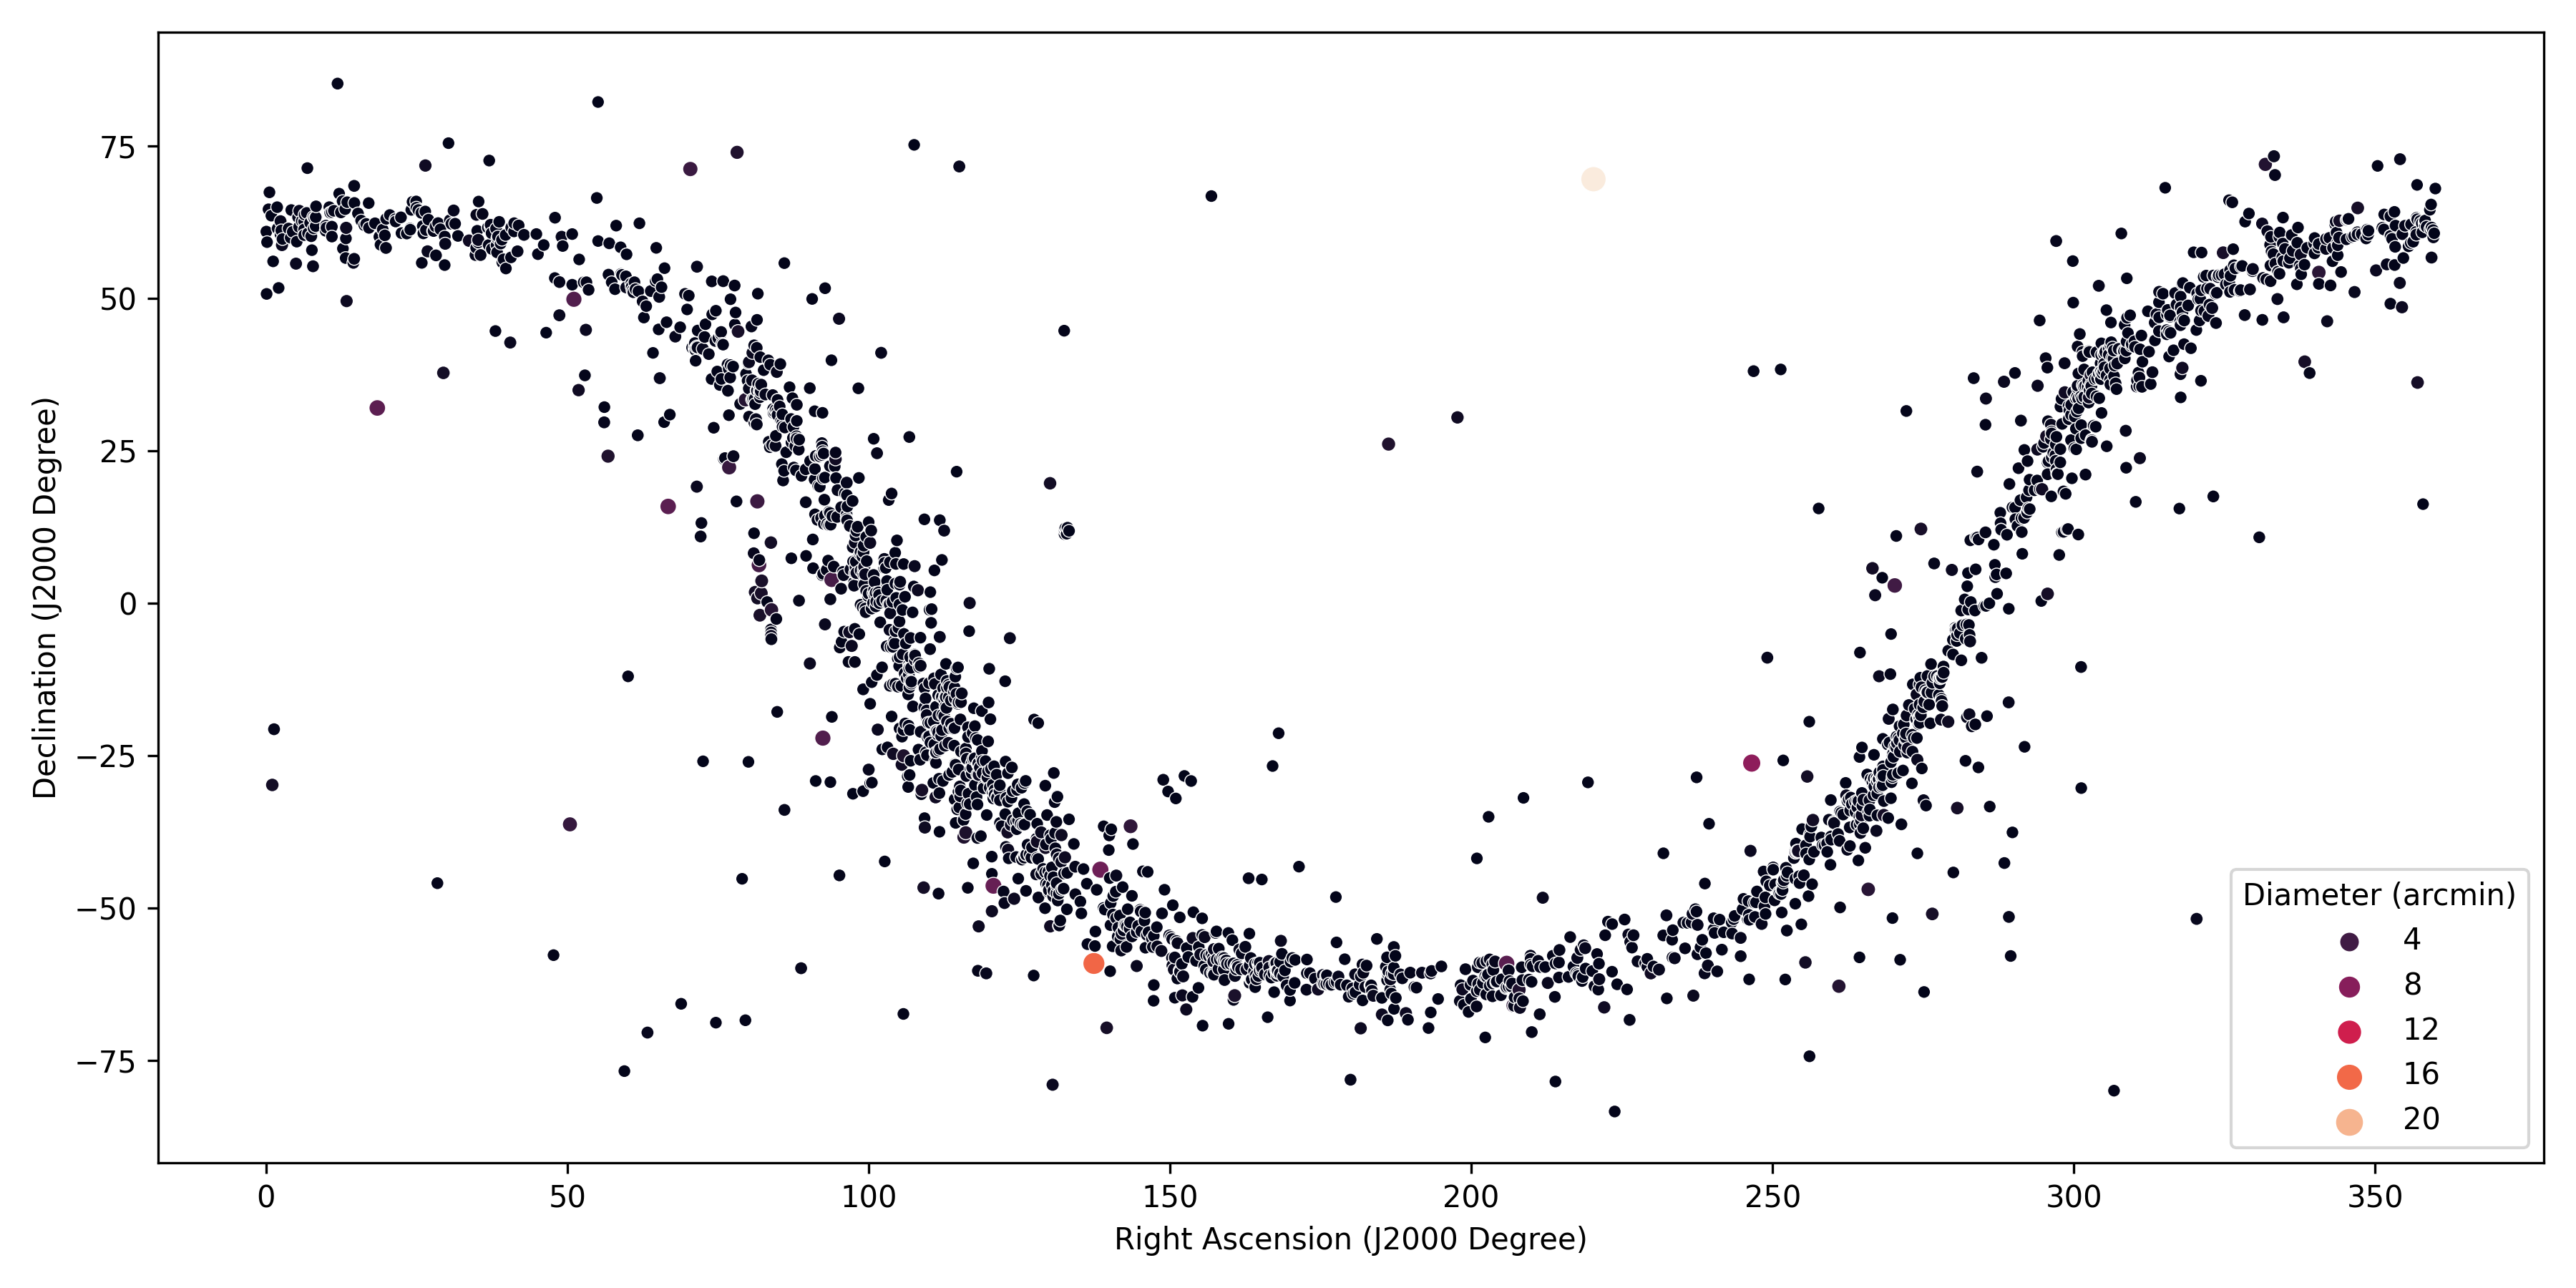
\includegraphics[width=\columnwidth]{../figures/openclust_catalogue.png}
    \caption{OpenClust Catalogue Distribution}
    \label{fig:openclust_catalogue}
\end{figure}

Finally, we have compared the results obtained with the model we purposed with another
method that involves tools from the Virtual Observatory (VO) such as Clusterix \cite{balaguer2020clusterix}.

As shown in Section \ref{sec:results}, the results obtained are promising.
This allows us to consider our model as a valid tool that could be part
of the standard set of tools for open clusters characterization.

\section{STATE OF THE ART}

The initial approach to find open clusters is by searching for overdensities
in the astrometric space of the galactic disk and a later identification of
possible OCs using photometric information \cite{castro2020hunting}.
However, although it looks simple, it is not. Here we face the problem that the
near field around the OC is composed of two kind of populations.
The first kind belongs to the membership stars of the OC (from tens or hundreds
to a few thousand) while the second one is composed by a background of stars
that do not belong to the OC (from tens to hundreds of thousands).
To find out which stars do belong to the OC is the problem we try to solve in
this work as this selection is critical to properly characterize the
fundamental properties of the cluster (total mass, age, chemical composition, etc.).

Since the components of the open cluster are born from the same gas cloud and they
share both dynamic properties and relative distance, as well as age and chemical
composition, the first step is to analyze the proper motion configuration space of
the region of interest. This approach is the one used by many tools from the VO
such as TOPCAT \cite{taylor2005topcat}, Clusterix 2.0 \cite{balaguer2020clusterix},
Aladin \cite{bonnarel2000aladin} or VOSA \cite{bayo2008vosa}.

TOPCAT by itself cannot find members of the open cluster. It requires to parameterize
some of the properties of the cluster, what requires a previous knowledge of the cluster.
Or to make a supervised and manual selection of groups based on overdensities
in the proper motion configuration space. Clusterix 2.0, an interactive web-based tool,
can help to this process. It takes the proper motion diagram without making any prior
assumption about the membership of the candidate star and determines empirically
the frequency functions. Clusterix uses normal Gaussian kernel functions, defined as:

\begin{equation*}
  K(a, b) = \frac{1}{2 \pi h^{2}} \exp{ \left[ - \frac{1}{2}\frac{\left( a - a_{i} \right)^{2} + \left( b - b_{i} \right)^{2}}{ h^{2}} \right]}
\end{equation*}

$\left( a, b \right)$ are referred to the proper motion configuration space,
while a point located in the center of the cell $\left( i, j \right)$
provides the maximum contribution for calculating the local density.
Number $h$ is called the \emph{smoothing} parameter and it is measured
in the same units as proper motion.

Clusterix is defined as an unsupervised and non-parameterized tool, but it
critically depends on the selection of three radii in the studied region.
The inner radius should contain stars belonging or not to the cluster.
While the outermost radii define a ring which only contains stars that do
not belong to the cluster. In addition, it is also sensitive to other
parameters, such as the soften parameter \emph{h}, or other restrictions
related with the searched proper motions.

If the analysis performed by Clusterix is successful, it returns the probability
associated to each star in the dataset to belong to the open cluster.
These results can be imported then into TOPCAT to continue the refining process to
get a valid characterization.

Another recent approach to solve this problem based on machine learning techniques
makes a systematic search for overdensities in the astrometric space of the galactic
disk and a subsequent identification of open clusters using photometric information
\cite{castro2020hunting}.

This last method includes two phases: the first one uses an unsupervised clustering
algorithm, DBSCAN, to search for overdensities $(l, b \pi, \mu_{\alpha} *, \mu_{\delta})$,
and then applies a deep learning ANN, previously trained with magnitude diagrams,
to identify isochrone patterns within the detected overdensities and thus proceed
to confirm them as OC.

It should be noted that for the execution of this method, MareNostrum 42
(Barcelona Supercomputing Center) was used.
So the neural network could handle the image recognition process with
isochrone patterns and not applying theoretical models derived from
values such as metallicity or masses, among other.

This work concludes with the identification of 582 new open clusters
distributed along the galactic disk for a galactic declination bellow 20 degrees.
This result increases the number of known open clusters by 45\%.

As told before, our aim in this work, linked to computational limitations compared
to MareNostrum, is not to do a blind search for clusters, but to obtain a method,
in the machine learning environment, that allows the characterization of open clusters.
We require our method to be unsupervised and non-parameterized making it suitable for
automated processes.

We use the Clusterix+TOPCAT method applied to the same clusters that we have analyzed
with our method to validate our results.

In this work we make use of Gaia DR2 since DR3 has not been released in time for us to include it.
Gaia DR2 is a multidimensional dataset obtained by ESA's Gaia mission
(located at L2, 1.5 million kilometers from Earth) and operational since 2014.
The catalogue has high precision and accuracy astrometric data for more than 1.7 billion stellar sources,
and magnitudes in three photometric filters (G, BP and RP) for more than 1,300 million sources.

As we will explain later, what we need to accomplish our aim is an algorithm
that manages to make data groups based on the dynamic properties of the stars.

There are several clustering algorithms: K-Means, Mean-Shift Clustering, DBSCAN \cite{ester1996density}
among other. While each one behaves better according to the distribution of the objects
to clusterize, we have chosen K-Means by its simplicity and good results.

This algorithm works well and gives good results at first approach.
However, we need to set a large number of clusters to find the open cluster we are looking for.
This fact complicates the identification of the OC and many times the found cluster contains to many outliers.
For that reason, we have search for a K-Means refinement based on an artificial neural network.

The \emph{Unsupervised Deep Embedding for Clustering Analysis} model
or \emph{DEC} \cite{xie2016unsupervised} takes K-Means as its starting point,
but then, it trains an autoencoder to reduce the feature space
and pass this transformed data through a Clustering Layer which refines the previous selection.

\section{AIMS AND METHOD}

Our aim is to \emph{build an unsupervised clustering model for open cluster characterization}.
The model will be \emph{non-supervised and non-parameterized} in order to fit a wide range
of clusters without the need for fine-tuning a high number of hyperparameters.

\subsection{DOWNLOAD}

We start by selecting a region from the OpenClust catalogue and downloading it from
Gaia DR2 database into a docker database. This allows us to repeat the analysis without
having to download the data every time. The radius of the downloaded region from Gaia
is 1.5 times larger than the one registered in OpenClust. This way we ensure to include
several stars that do not belong to the open cluster.

\subsection{FEATURE SELECTION}
\label{sec:feature_selection}

\begin{figure}[htbp]
  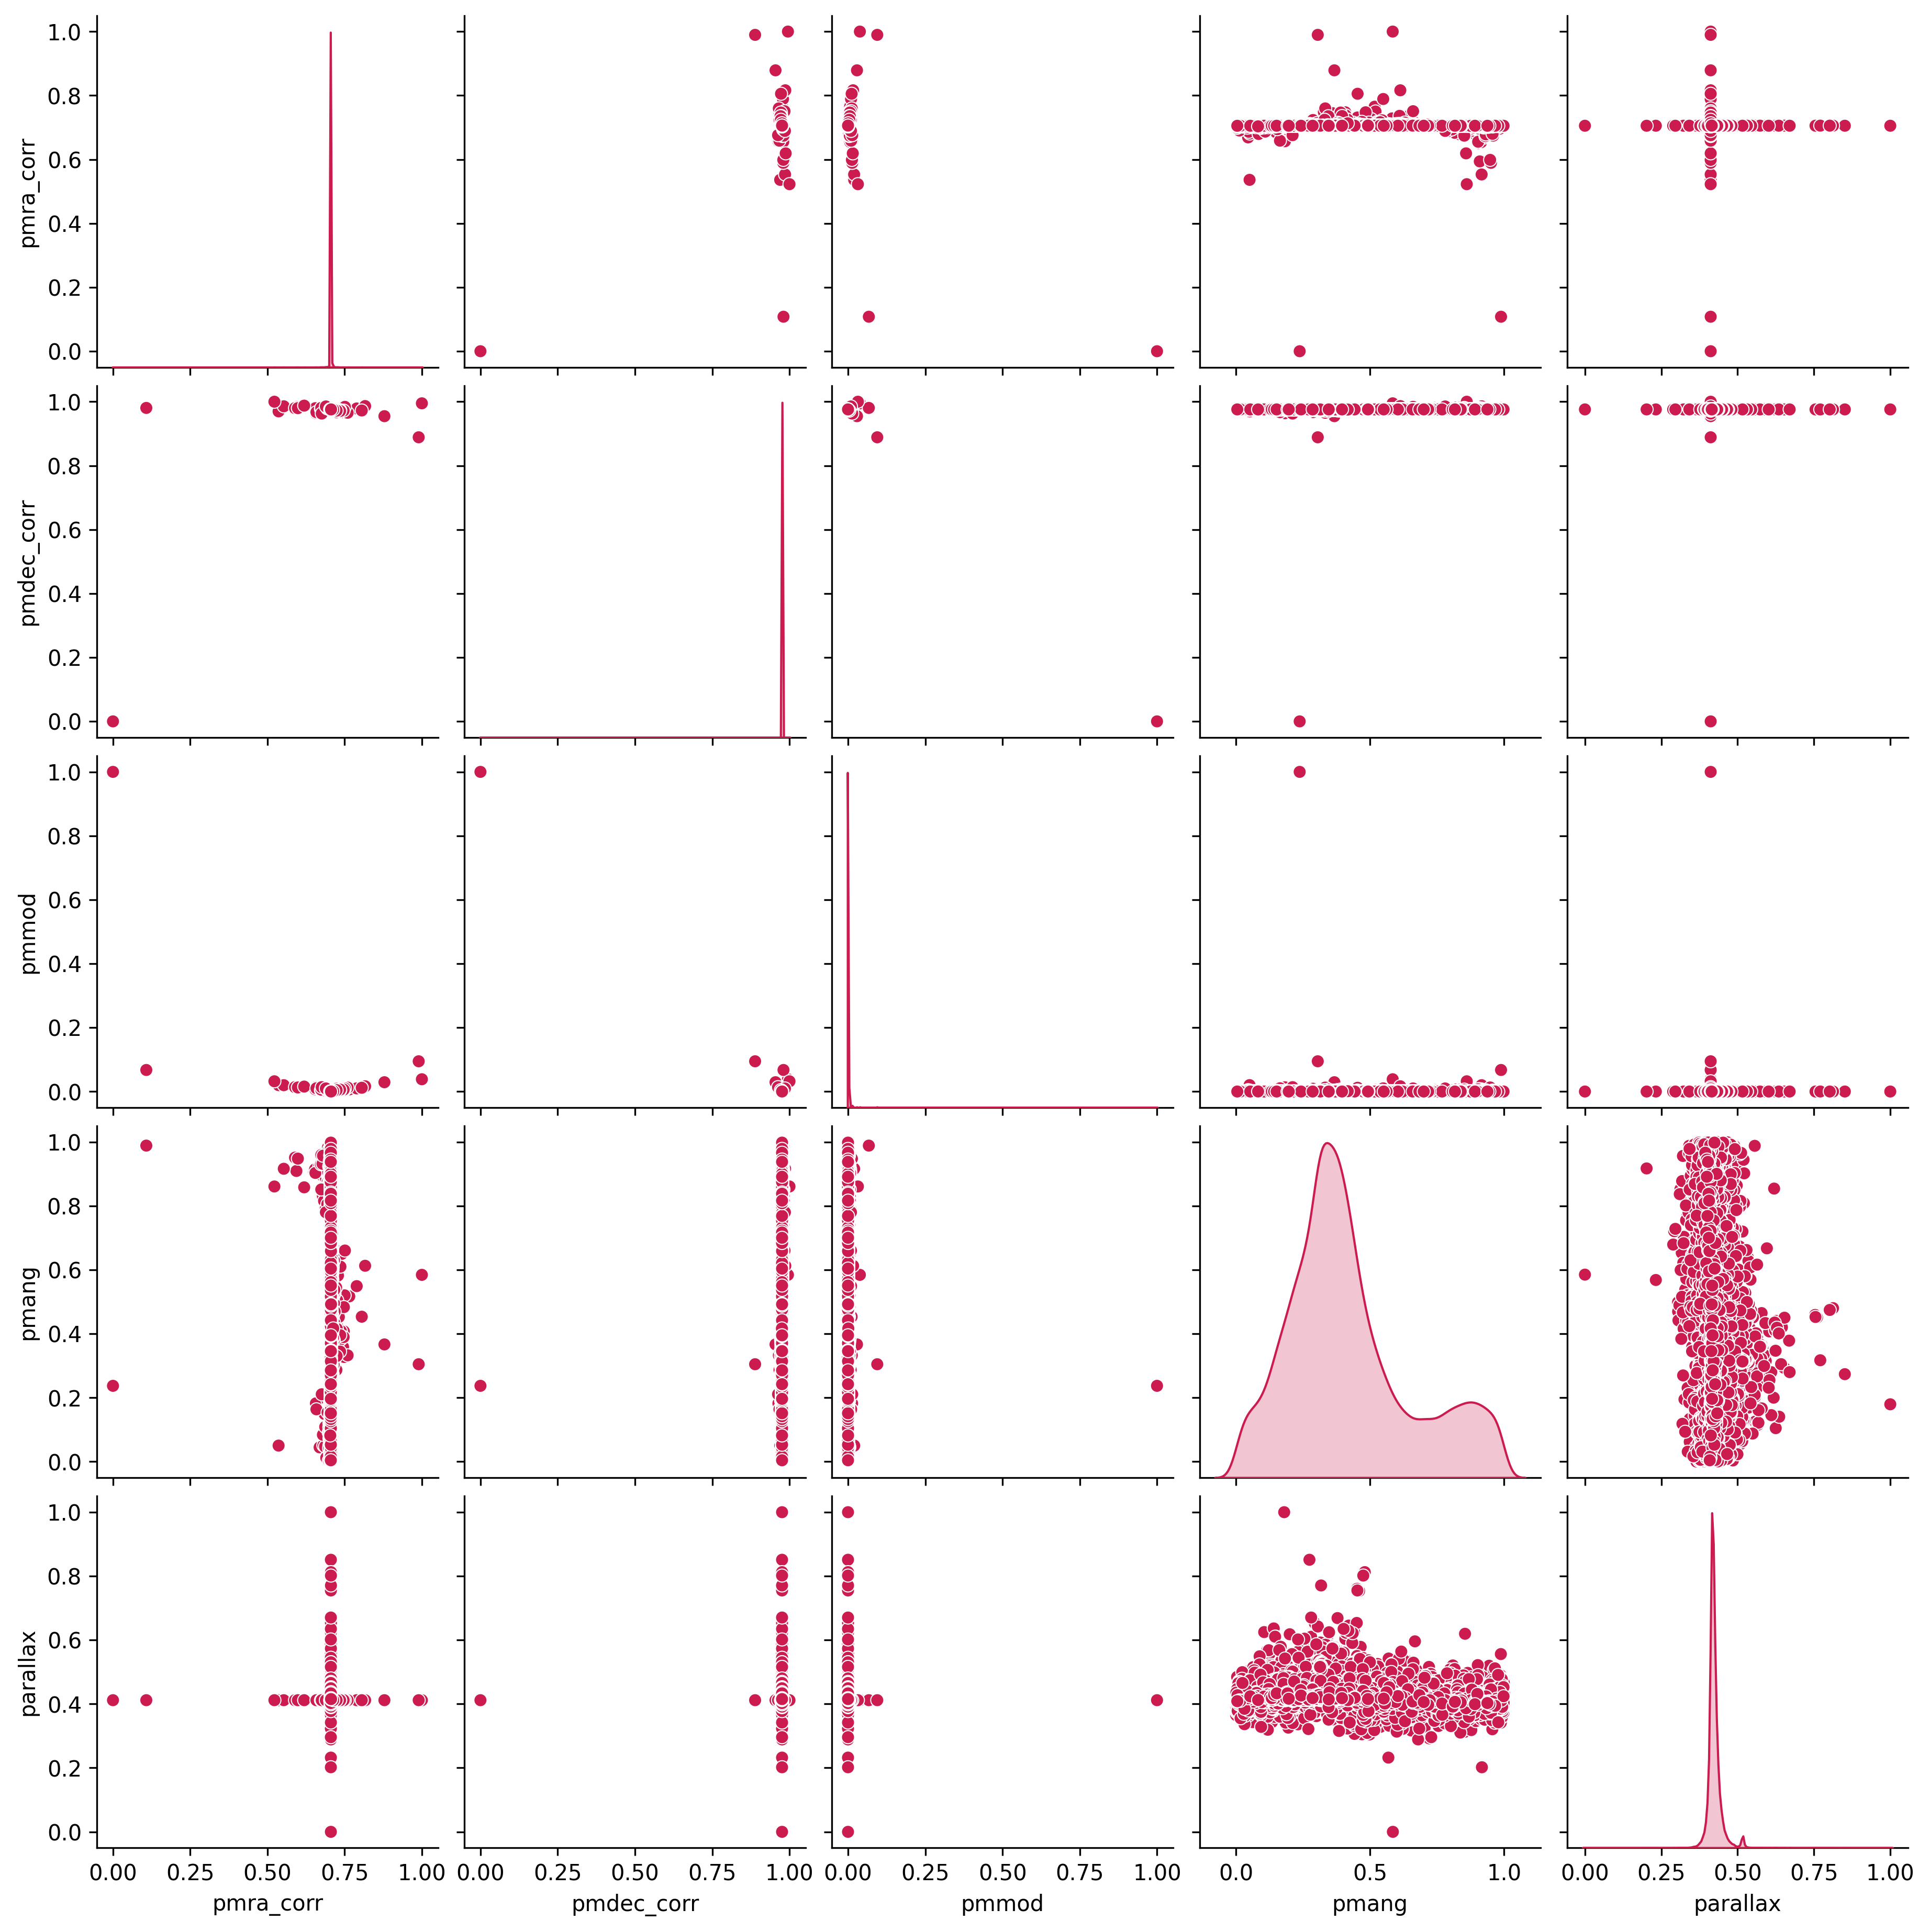
\includegraphics[width=\columnwidth]{../figures/melotte_22/features_melotte_22.png}
  \caption{Pairwise relationships among variables using Melotte 22 data}
  \label{fig:features_melotte_22}
\end{figure}

As mentioned before, we want our model to characterize open clusters by looking at
their dynamic properties. Also, we want to maintain as simple as possible our
clustering model in order to save computing resources.

Proper motion in right ascension and declination seems like a natural choice since,
as we know, stars belonging to the same OC share a common motion vector.

Parallax is another important feature. It lets us know how far stars are from us.
In addition, since all stars within an open cluster were born from the same dust cloud,
they must all have similar parallax.

However, we are not going to use these raw features.
Instead, we are taking a combination of them.

First, we correct proper motion in right ascension and declination by dividing them by
the parallax. That way, we normalize these quantities and help our clustering models
to improve their performance.

The modulus of the proper motion is another computed property that we are considering.
We use it to relate both features and therefore, to force our model to keep them tight.

Figure \ref{fig:features_melotte_22} shows a pairwise relationship among some features
available in the dataset for Melotte 22 data.

\subsection{SOFT CLUSTERING}

Our first approach to find the open cluster is using the K-Means algorithm.
Since we are looking for a single cluster, it seems reasonable to use a clustering
algorithm and set it to find two clusters. One for the desired OC and another which
contains stars that do not belong to the open cluster.
However, this idea is not completely right.

This is due to the fact that OC's stars are surrounded by other stars with possibly similar
properties. Therefore, setting the number of clusters to two is too low to separate them properly.

\begin{figure}
  \centering
  \begin{subfigure}{\columnwidth}
    \centering
    \begin{subfigure}[t]{0.3\textwidth}
      \centering
      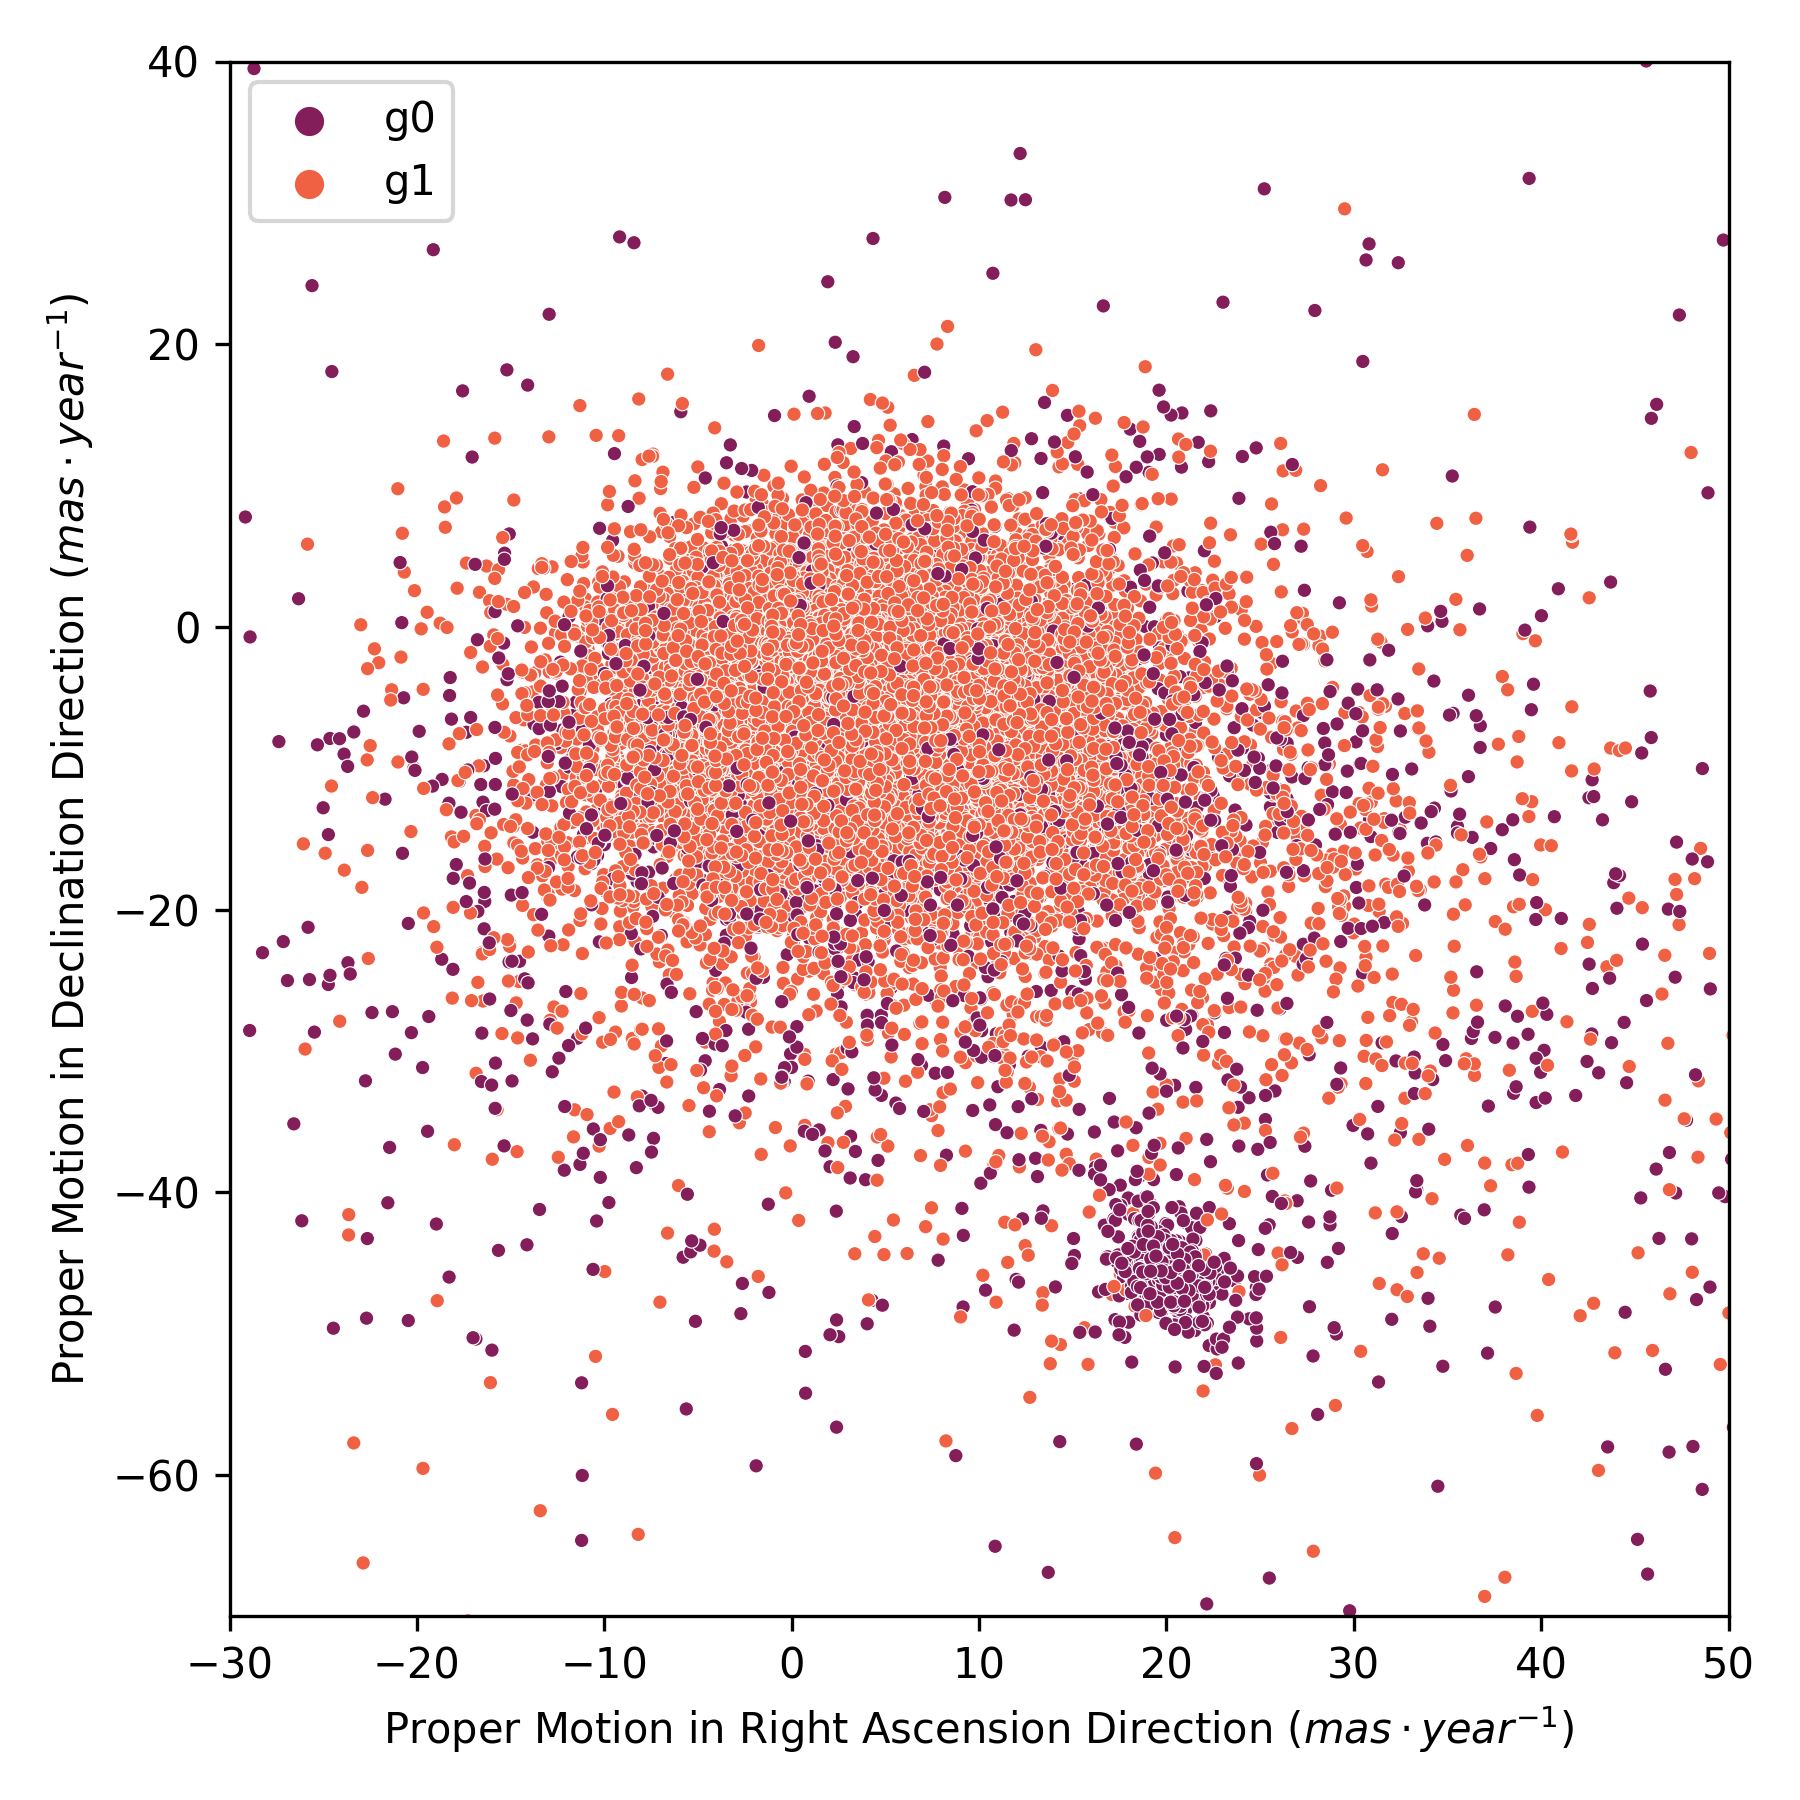
\includegraphics[width=\textwidth]{../figures/kmeans/kmeans_n2_pm_melotte_22.png}
    \end{subfigure}
    \hfill
    \begin{subfigure}[t]{0.3\textwidth}
      \centering
      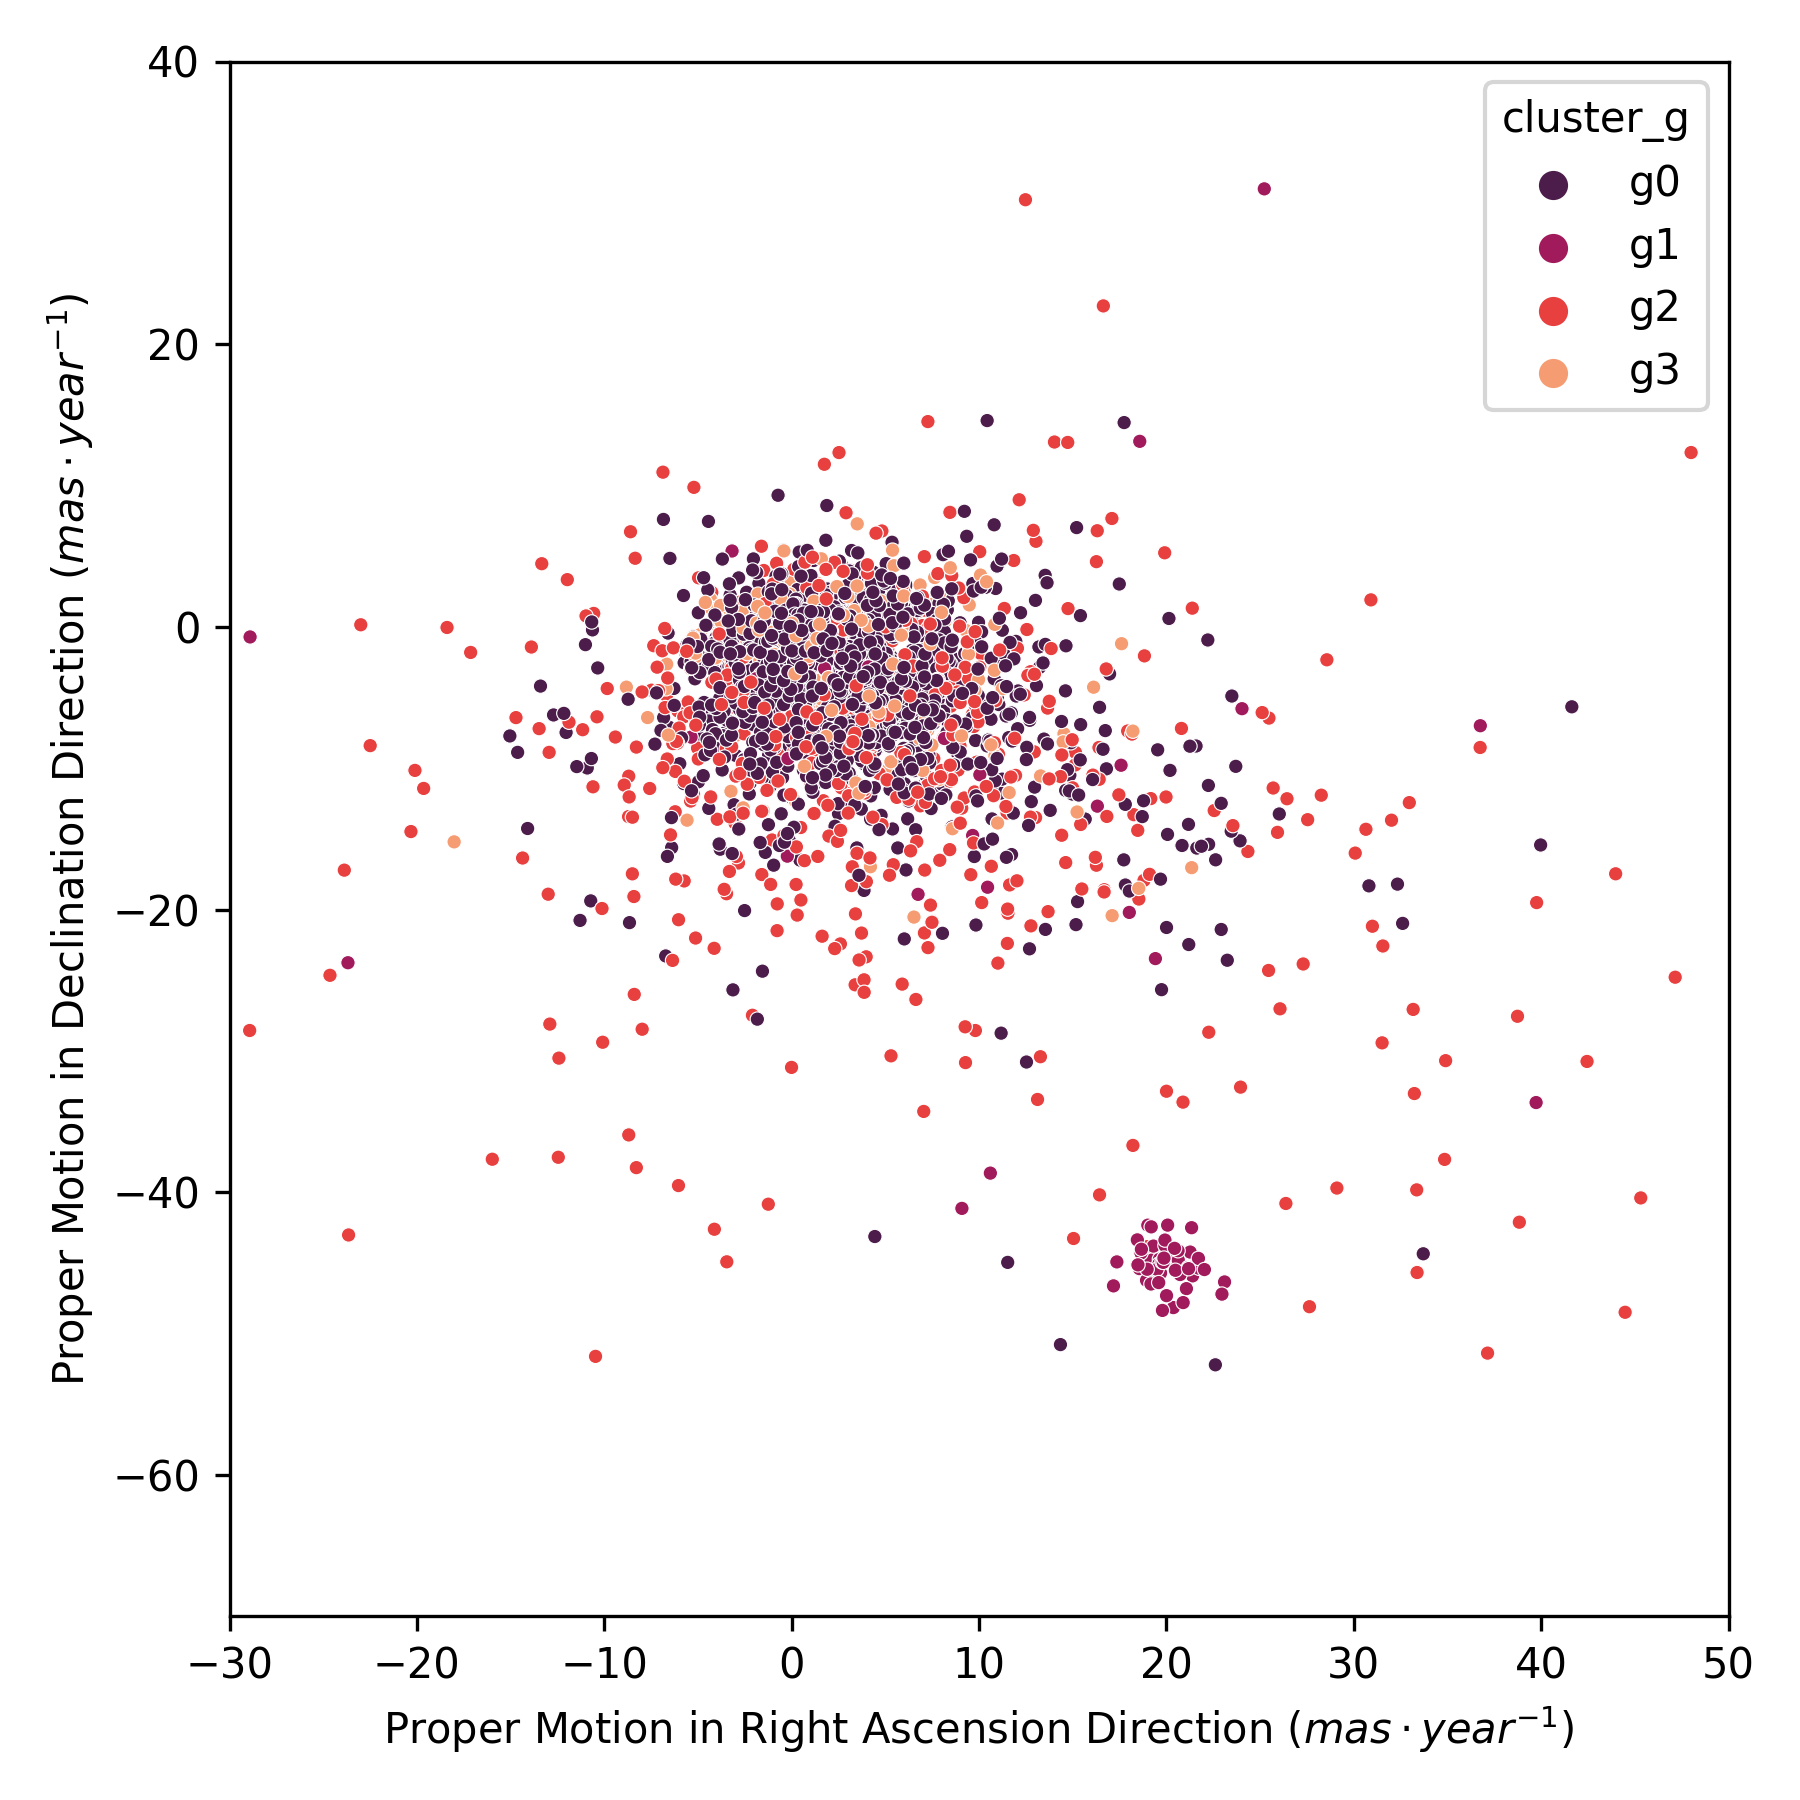
\includegraphics[width=\textwidth]{../figures/kmeans/kmeans_n5_pm_melotte_22.png}
    \end{subfigure}
    \hfill
    \begin{subfigure}[t]{0.3\textwidth}
      \centering
      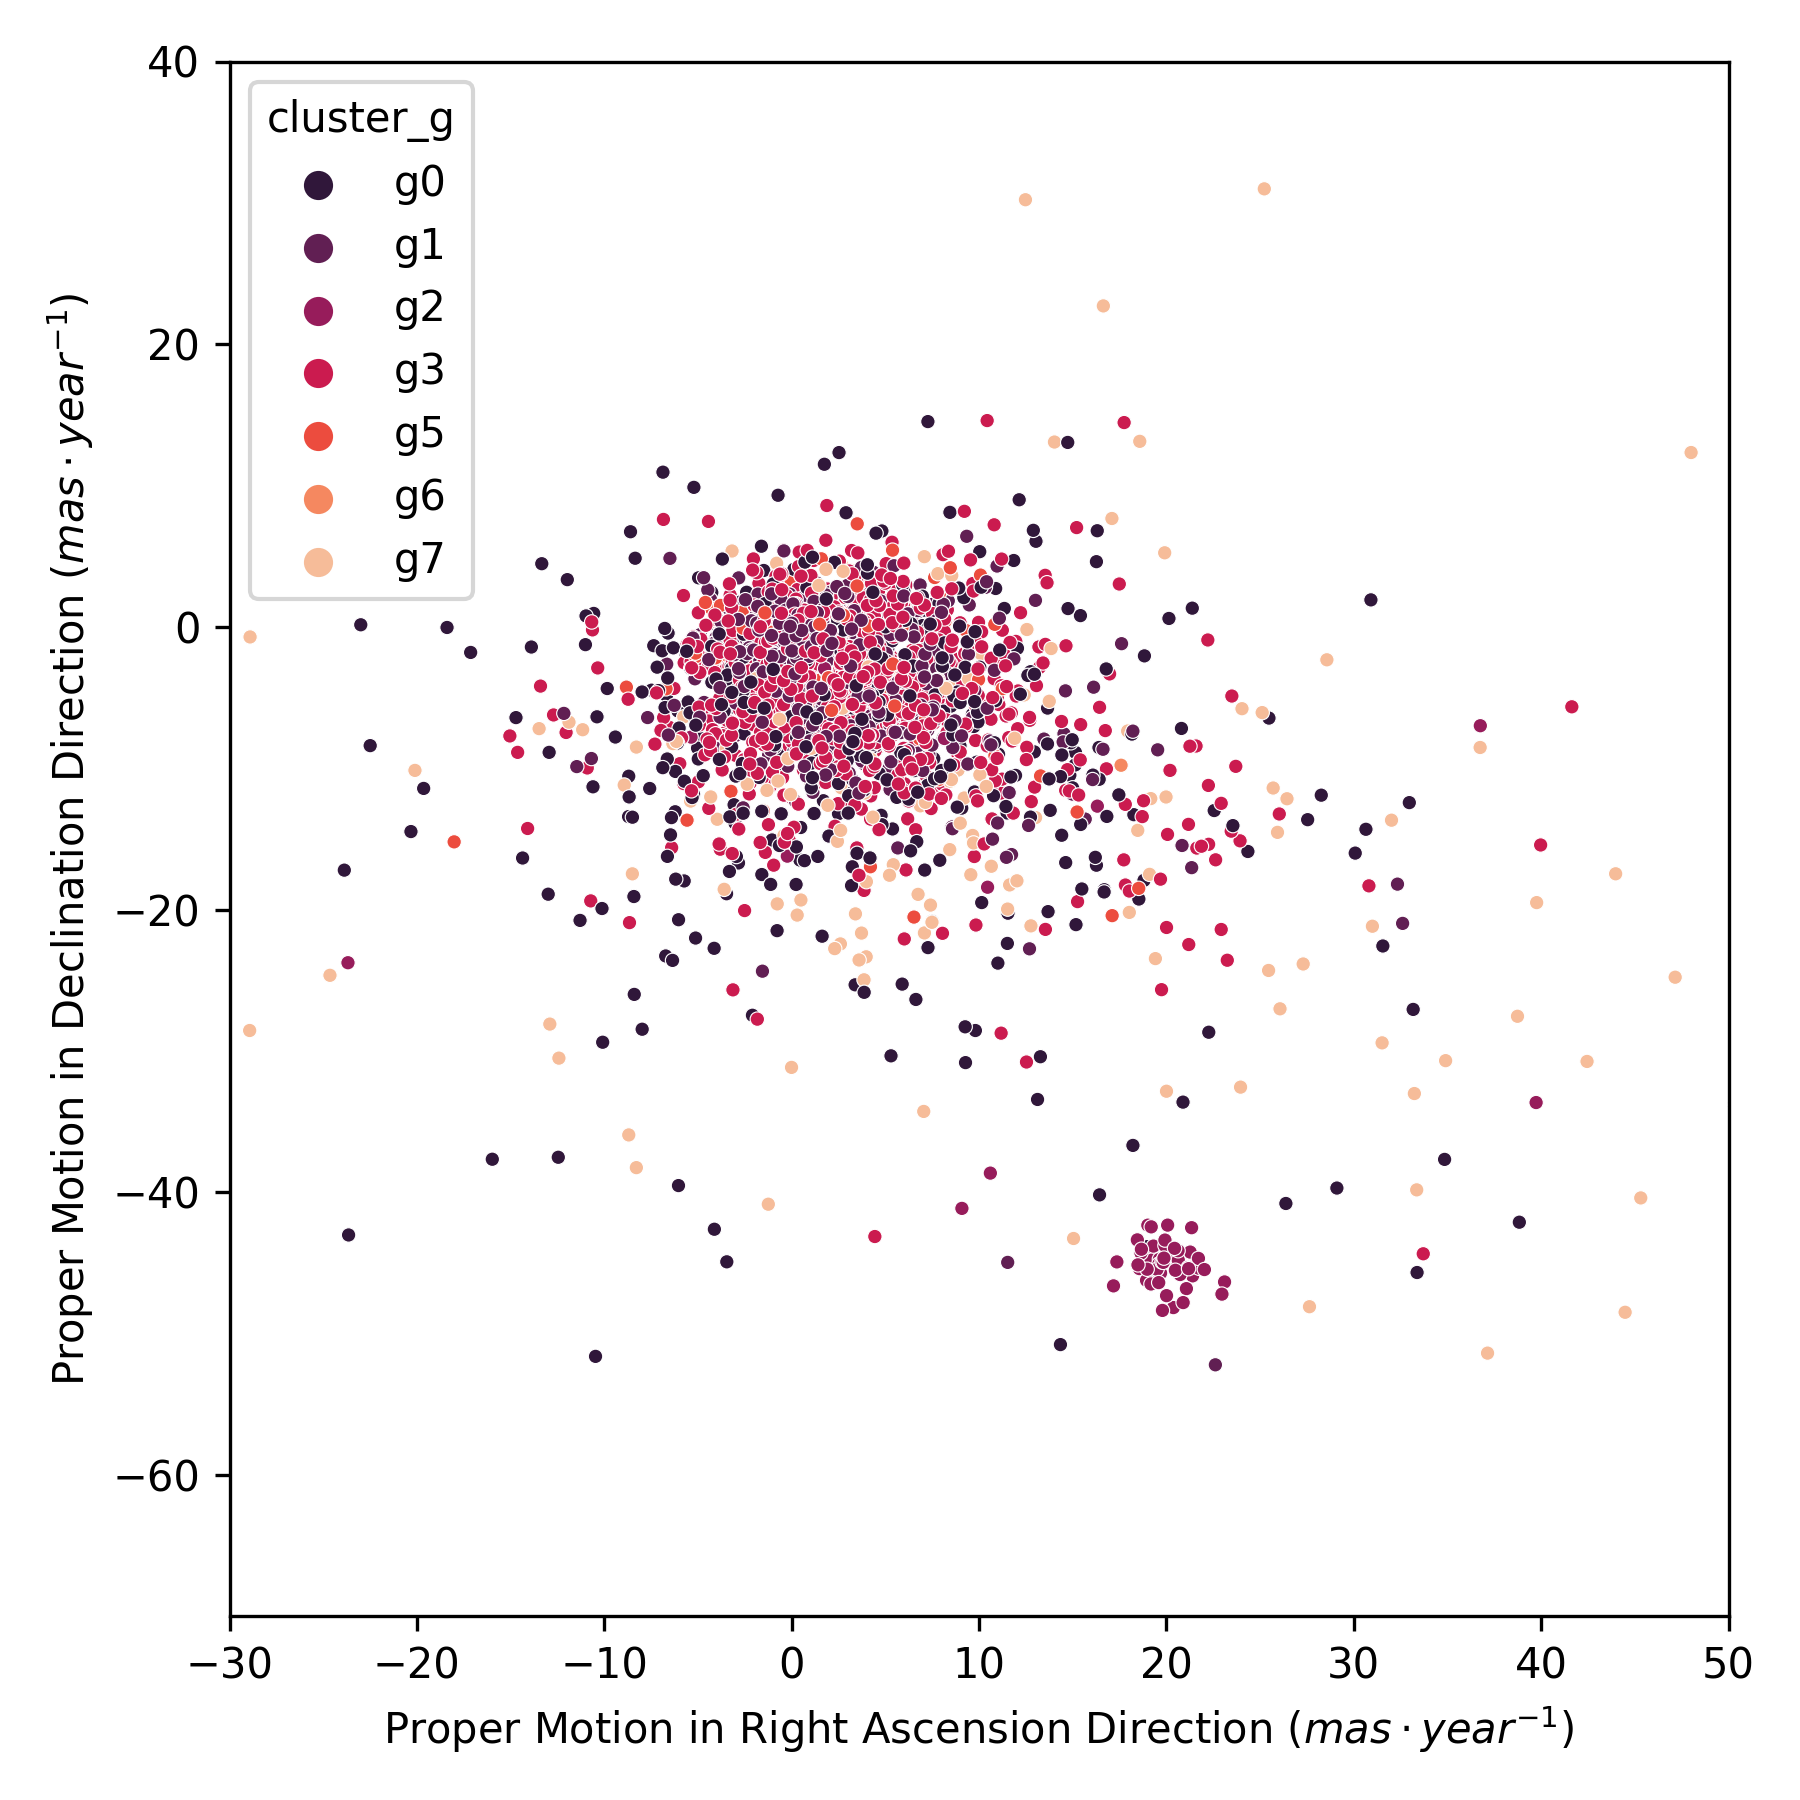
\includegraphics[width=\textwidth]{../figures/kmeans/kmeans_n8_pm_melotte_22.png}
    \end{subfigure}
  \end{subfigure}
  \medskip
  \begin{subfigure}{\columnwidth}
    \centering
    \begin{subfigure}[t]{0.3\textwidth}
      \centering
      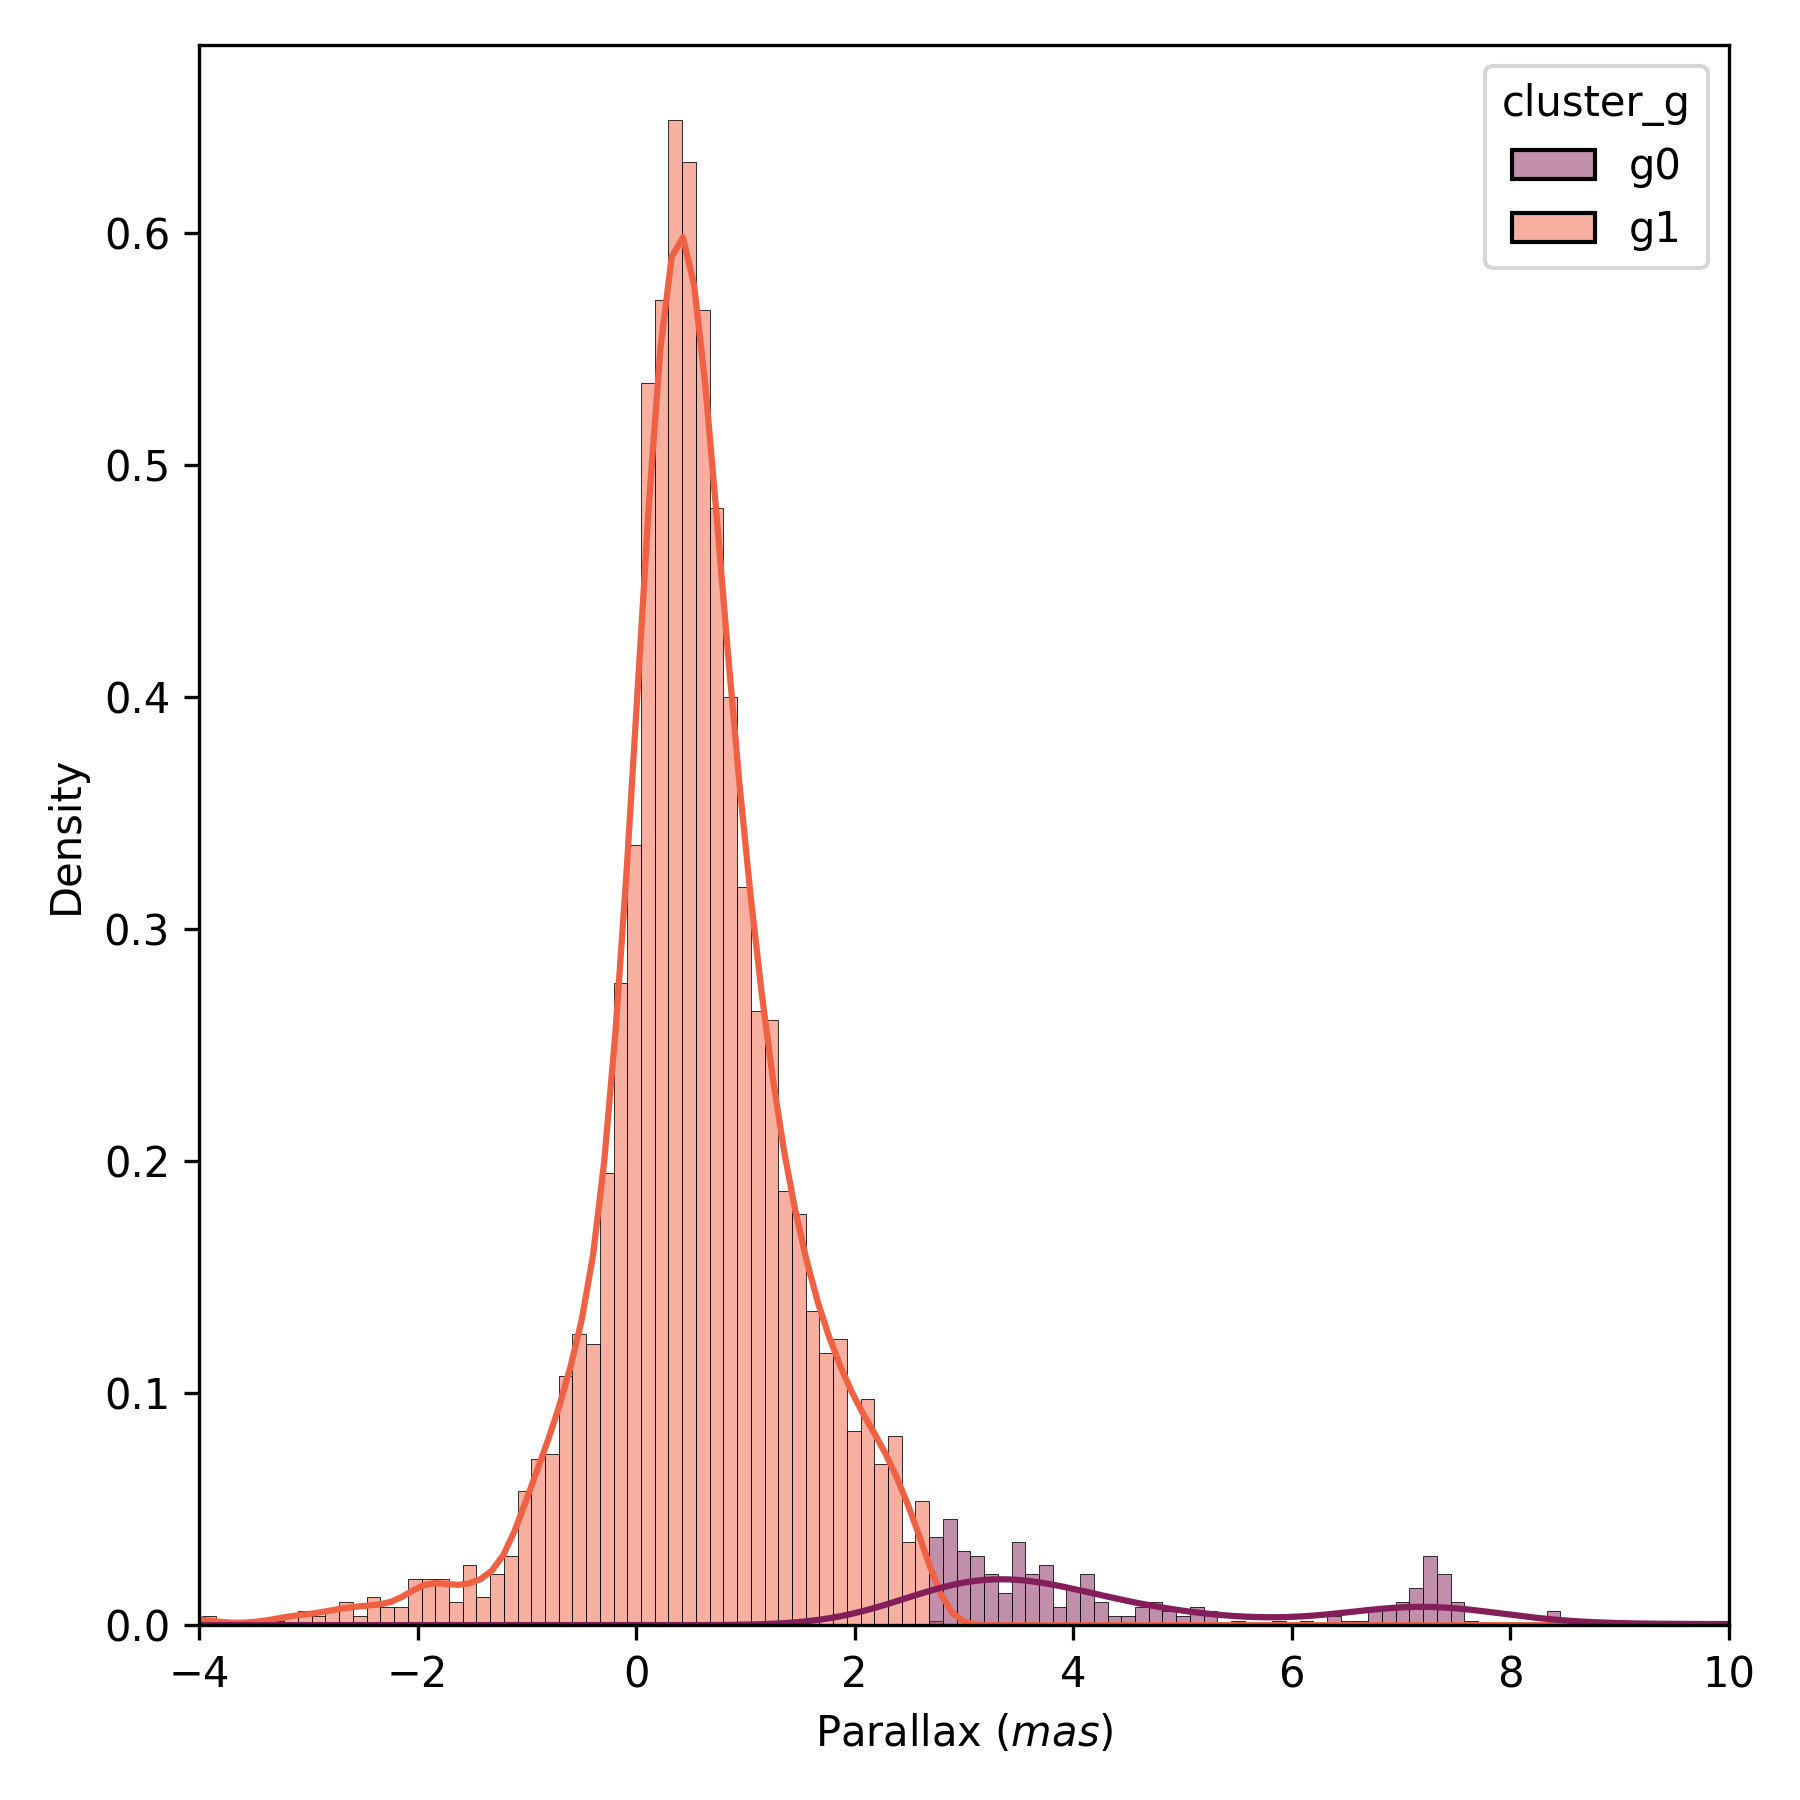
\includegraphics[width=\textwidth]{../figures/kmeans/kmeans_n2_parallax_melotte_22.png}
      \caption{N = 2}
    \end{subfigure}
    \hfill
    \begin{subfigure}[t]{0.3\textwidth}
      \centering
      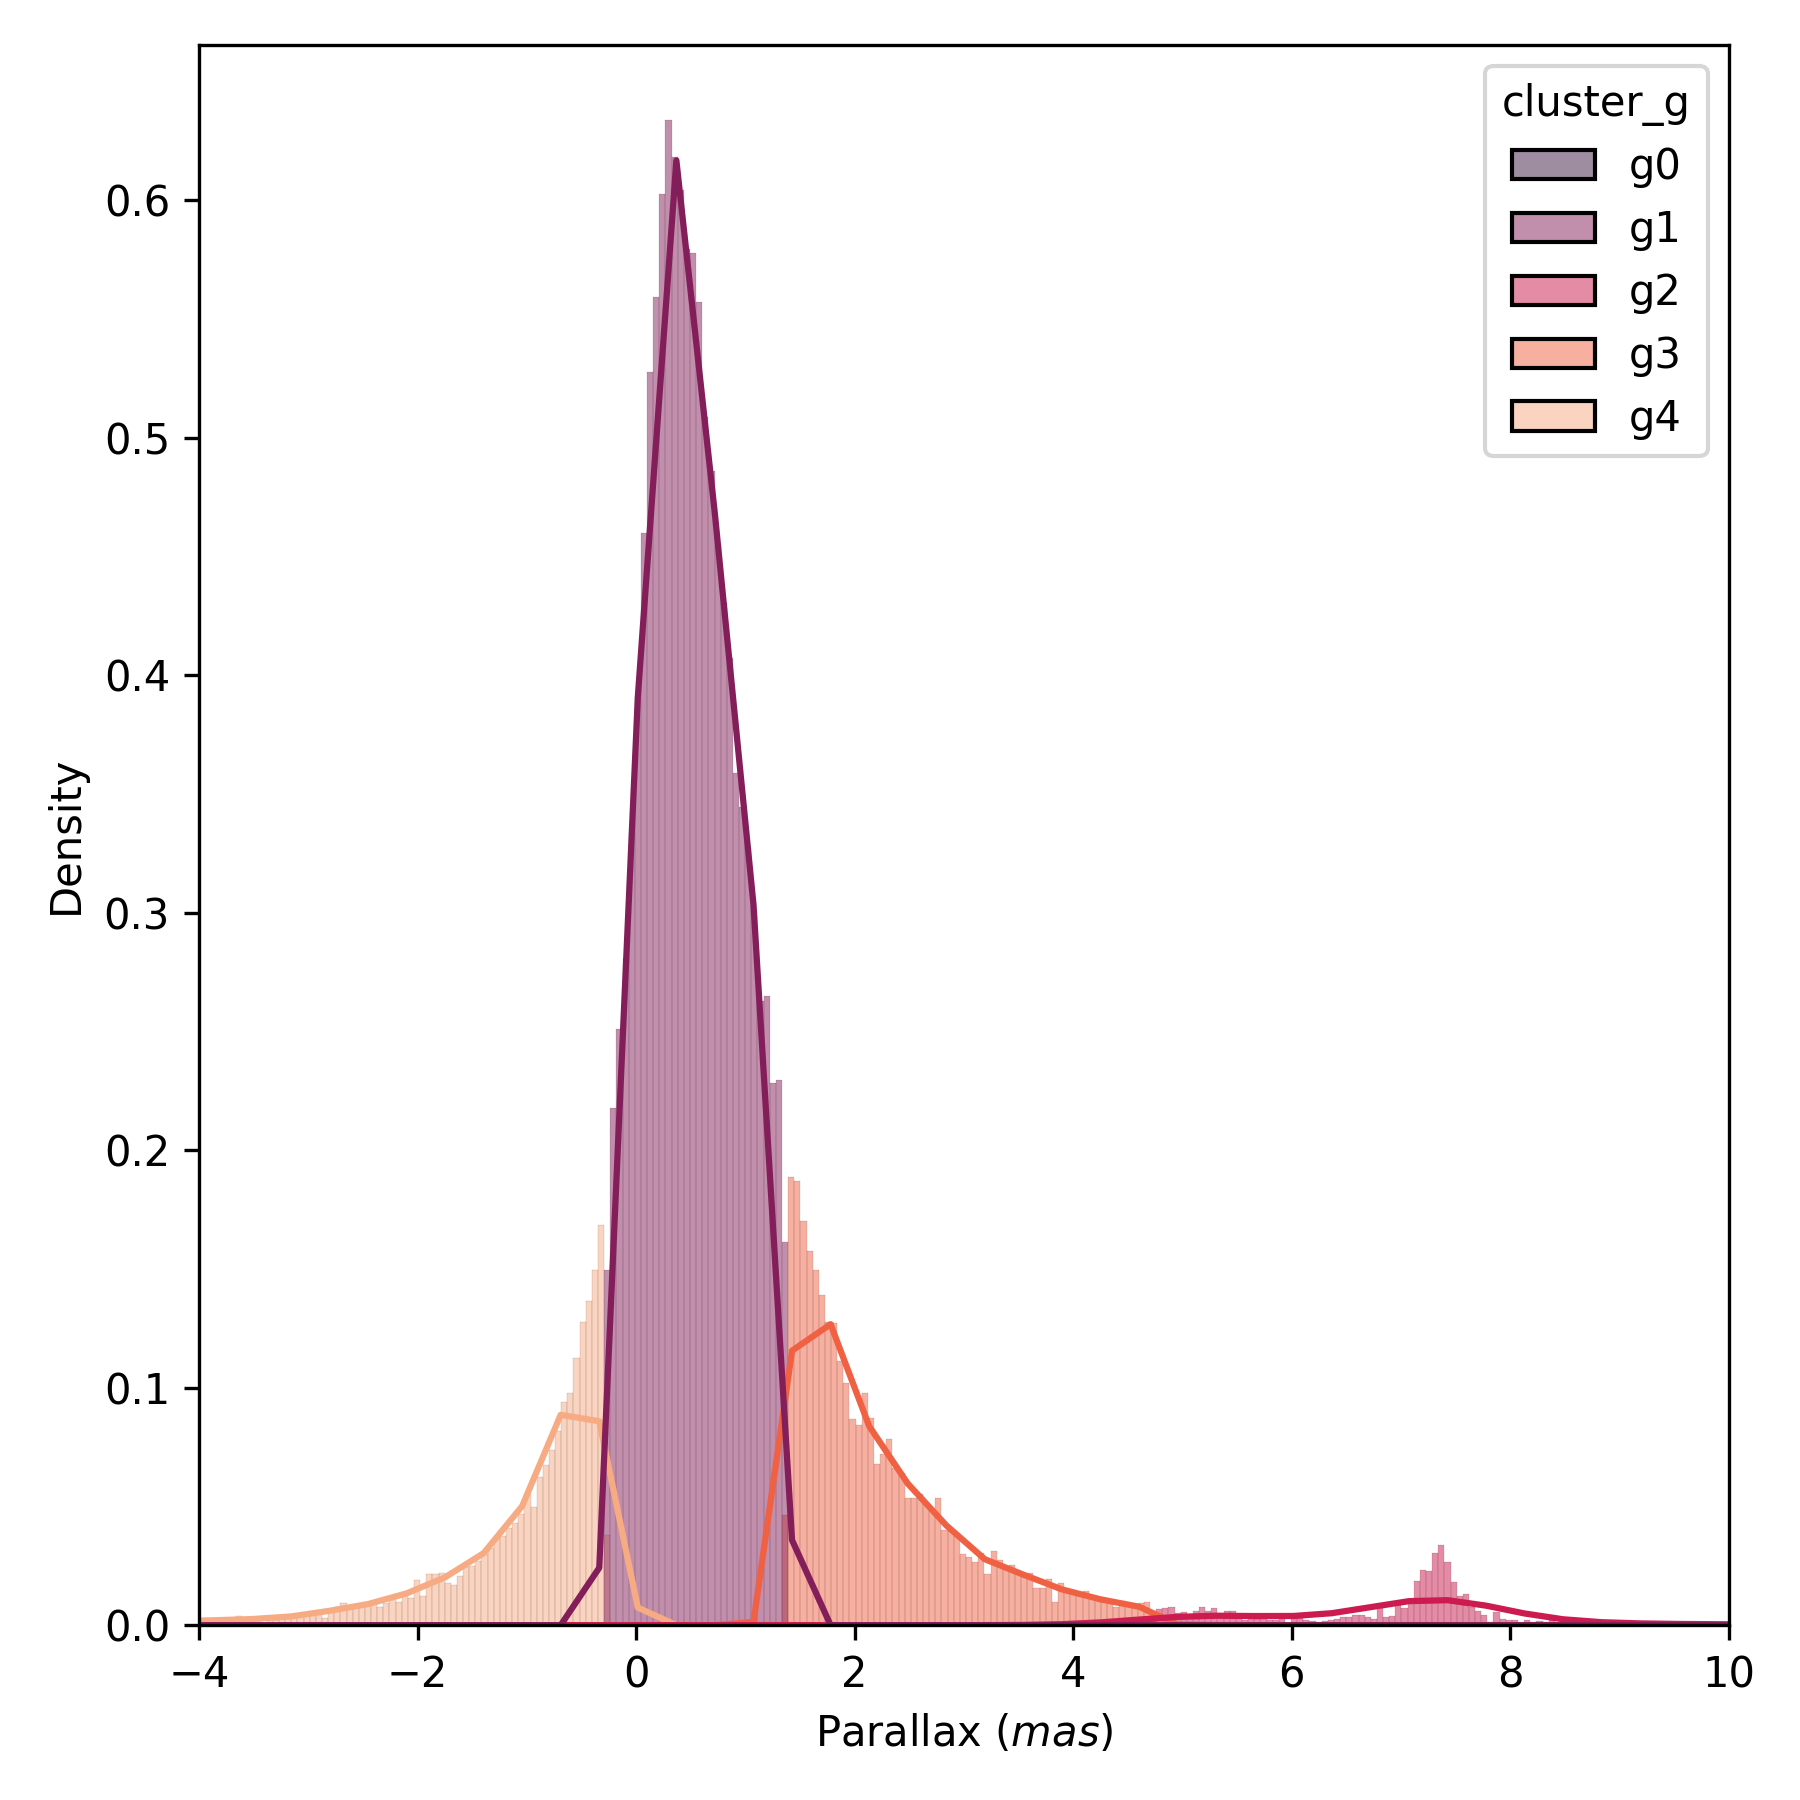
\includegraphics[width=\textwidth]{../figures/kmeans/kmeans_n5_parallax_melotte_22.png}
      \caption{N = 5}
    \end{subfigure}
    \hfill
    \begin{subfigure}[t]{0.3\textwidth}
      \centering
      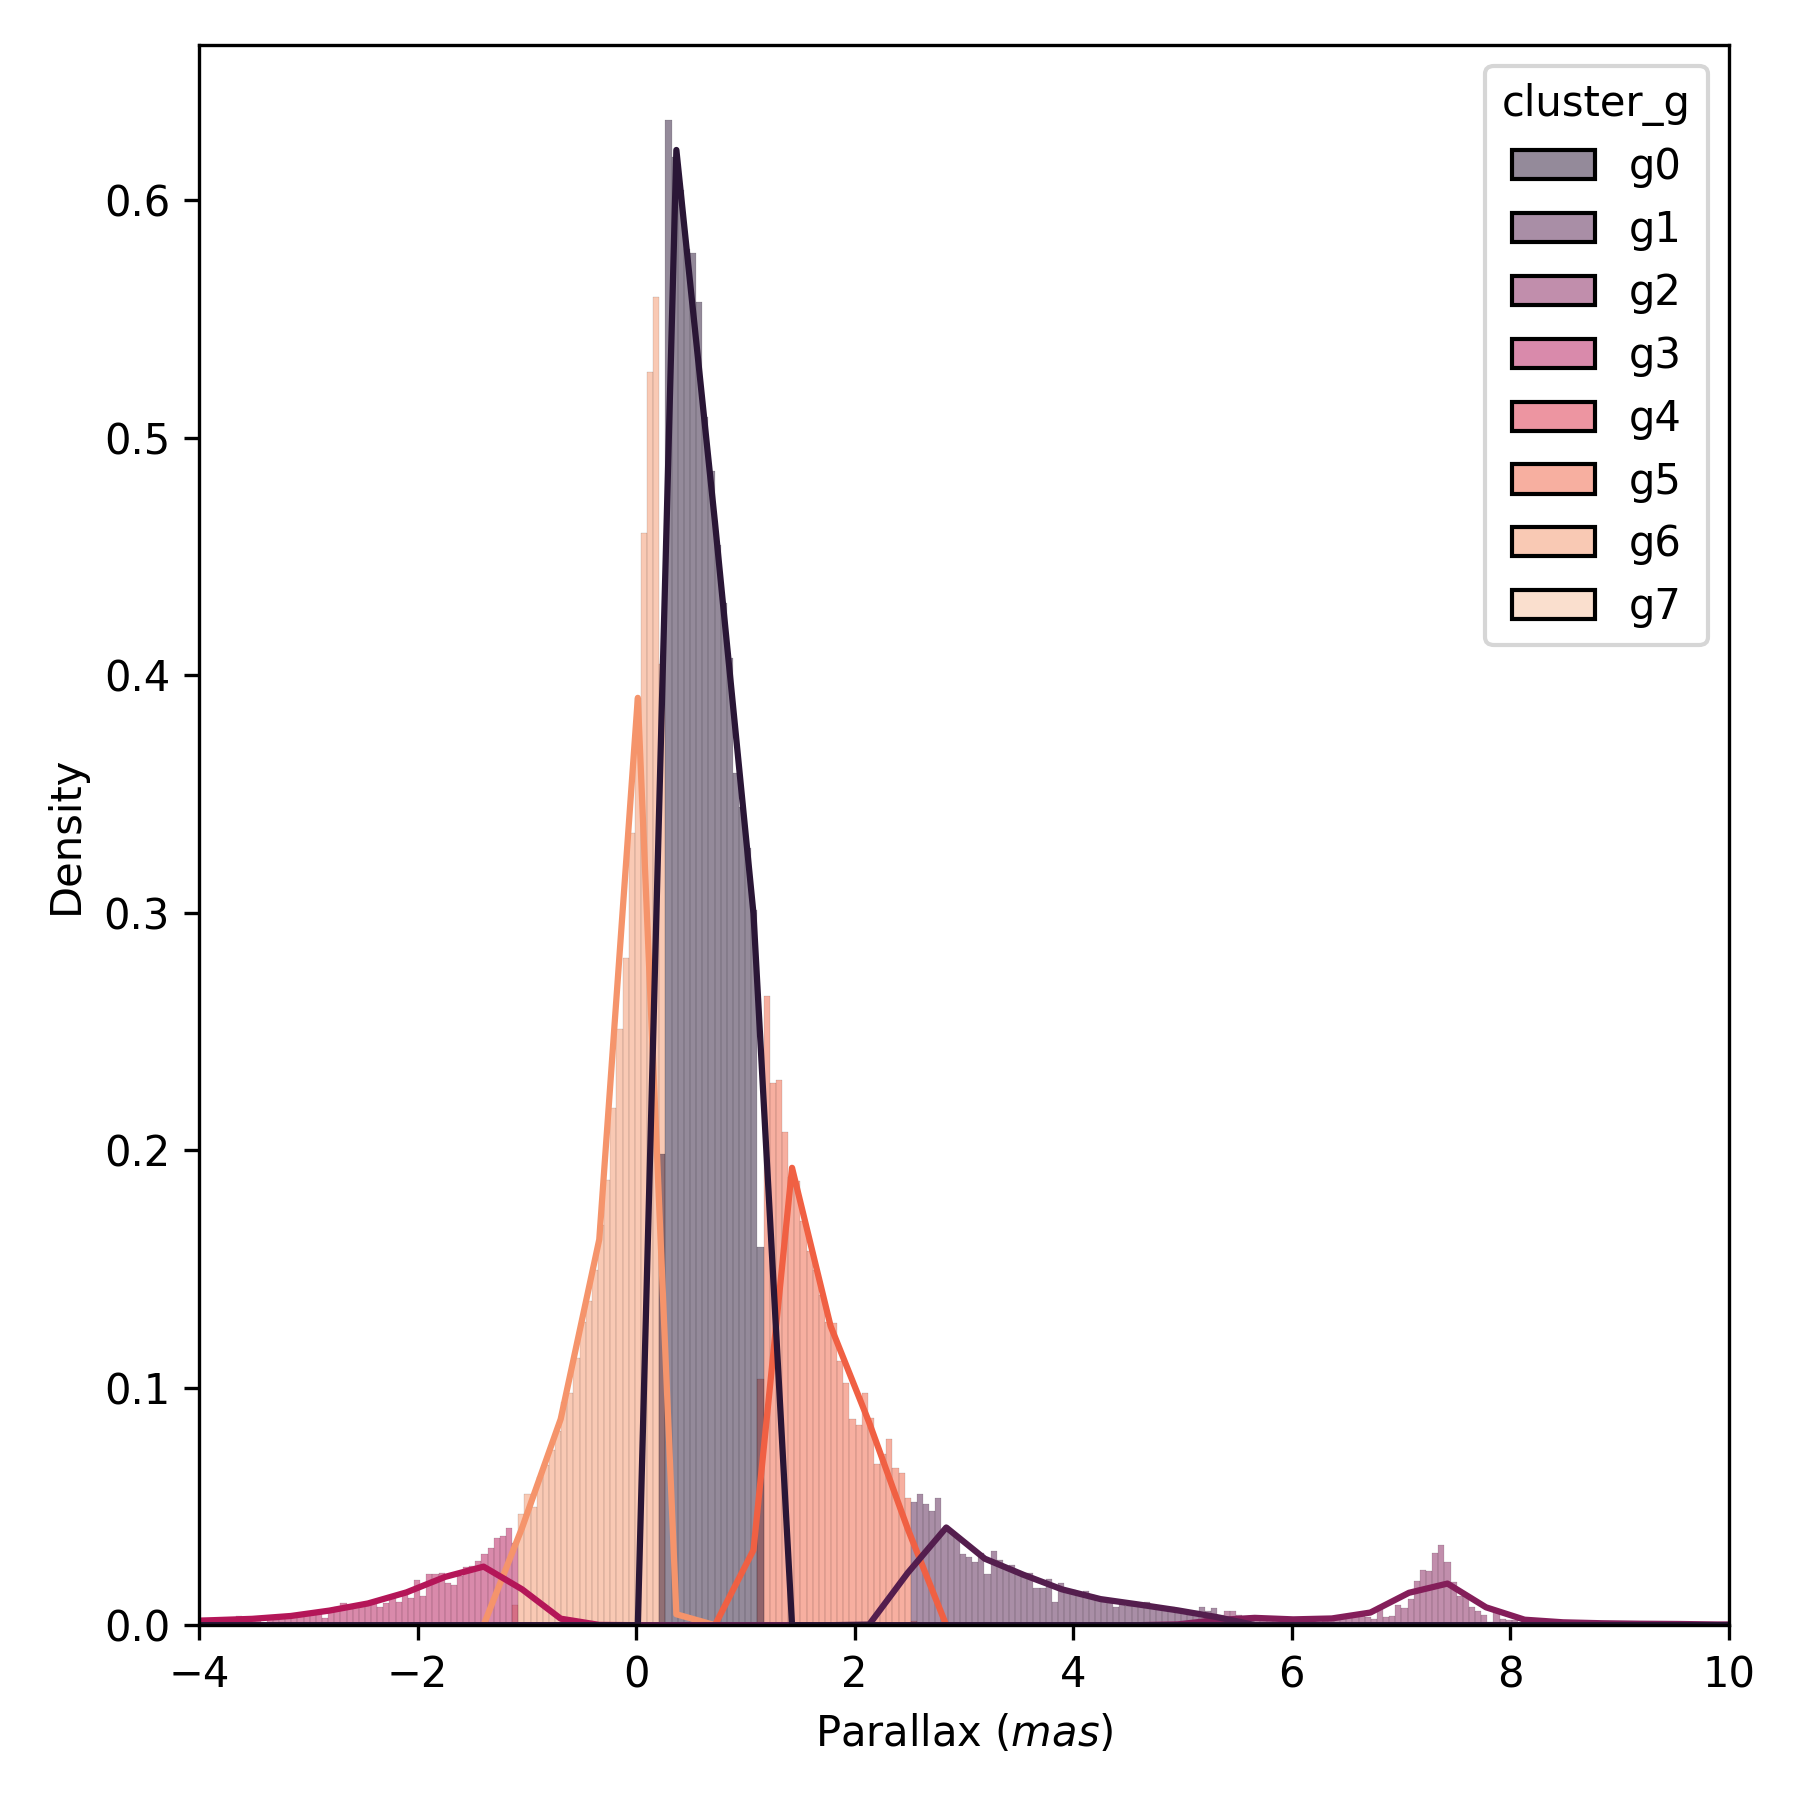
\includegraphics[width=\textwidth]{../figures/kmeans/kmeans_n8_parallax_melotte_22.png}
      \caption{N = 8}
    \end{subfigure}
  \end{subfigure}
  \caption{K-Means comparisons with Melotte 22}
  \label{fig:kmeans_comparisons_melotte_22}
\end{figure}

As shown in Figure \ref{fig:kmeans_comparisons_melotte_22}, larger values for the number of
clusters allow us to isolate more accurately the resonance in parallax at $\approx 7.3mas$.
However, we have the disadvantage that more groups are formed.

This effect complicates our task of finding the desired open cluster, since we would like
to get just two groups, one for the OC and another with the remaining stars.
Therefore, we have to find a way to set the right value for the number of clusters
to isolate the searched cluster without creating too many groups.

To solve this issue, we will try to estimate the best number of clusters by using the
\emph{silhouette score} \cite{rousseeuw1987silhouettes}.

K-Means does a good job making an initial clustering. However, too many clusters arise
from this characterization and the OC is still polluted with stars that do not belong to it.
Moreover, we would like to reduce the amount of clusters too.

Therefore, we would like to find a better model that improves this initial characterization
by reducing the amount of clusters and also that removes outsiders from the OC.

\subsection{DEC MODEL}

Since we do not have a labeled dataset to train a supervised model,
we have no choice but to use an unsupervised self-trained model.

For that reason we have adapted the \emph{Unsupervised Deep Embedding for Clustering Analysis}
to our work.

The model is composed by a \emph{deep autoencoder}, a \emph{deep encoder} and
a \emph{clustering layer}.

Encoders are used to transform the input data into a latent space
using a non-linear mapping function $f_{\theta} : X \rightarrow Z$.

Although, as explained in section \ref{sec:feature_selection},
the number of features we are managing is not too large,
this latent space helps us reduce the number of features
and avoids the \emph{"curse of dimensionality"} \cite{bellman1961curse}.

These encoders are pretrained before fitting the model to generate predictions. Then,
the encoder is used with the aim of transforming input data to the latent space $Z$. Once the
data has been transformed, a K-Means clusterer is used in order to make an initial clustering.

With that initial configuration, the model iterates alternating between computing an auxiliary
target distribution (Soft Assignment) and minimizing the Kullback-Leiber (KL) divergence
\cite{kullback1951information} to it. This unsupervised algorithm allows us to improve the clustering.

\begin{equation}
  p_{ij} = \frac{q^{2}_{ij} / f_{j}}{\sum_{j'}q^{2}_{ij'}/f_{j'}}
  \label{eq:student_tdistribution}
\end{equation}

In the soft assignment stage,
the \emph{Student's t-distribution} is used as a kernel to measure the similarity
between the embedded points and the cluster centroid.
While in the KL divergence minimization the algorithm iteratively refines clusters by learning
from their high confidence assignments with the help of an auxiliary target distribution.
The model is trained by matching the soft assignment to the target distribution.
The choice of this target distribution is crucial for DEC's performance.
In this work we have taken the target distribution from DEC's original paper \cite{xie2016unsupervised},
which is defined in Equation \ref{eq:student_tdistribution}.

Figure \ref{fig:dec_model_setup} shows the layer setup of our DEC model.
It is simpler than the one tested on the original paper \cite{xie2016unsupervised},
since the number of selected features in our work is smaller than in the original one.
Therefore, using the same configuration would result in a model so
powerful that would incur in overfitting issues unable to make right predictions.

\begin{figure}
  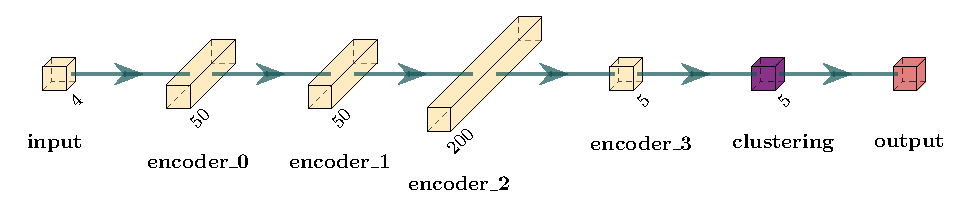
\includegraphics[width=\columnwidth]{../figures/dec_diagram.pdf}
  \caption{DEC model layer setup}
  \label{fig:dec_model_setup}
\end{figure}

Finally, we can refine this selection by filtering those stars which are bellow and above
the 0.10 and 0.90 quantiles for each group, respectively.
That way we remove the most doubtful values from the selection.

\begin{figure}[htbp]
  \centering
  \begin{subfigure}{\columnwidth}
    \centering
    \begin{subfigure}[t]{0.3\textwidth}
      \centering
      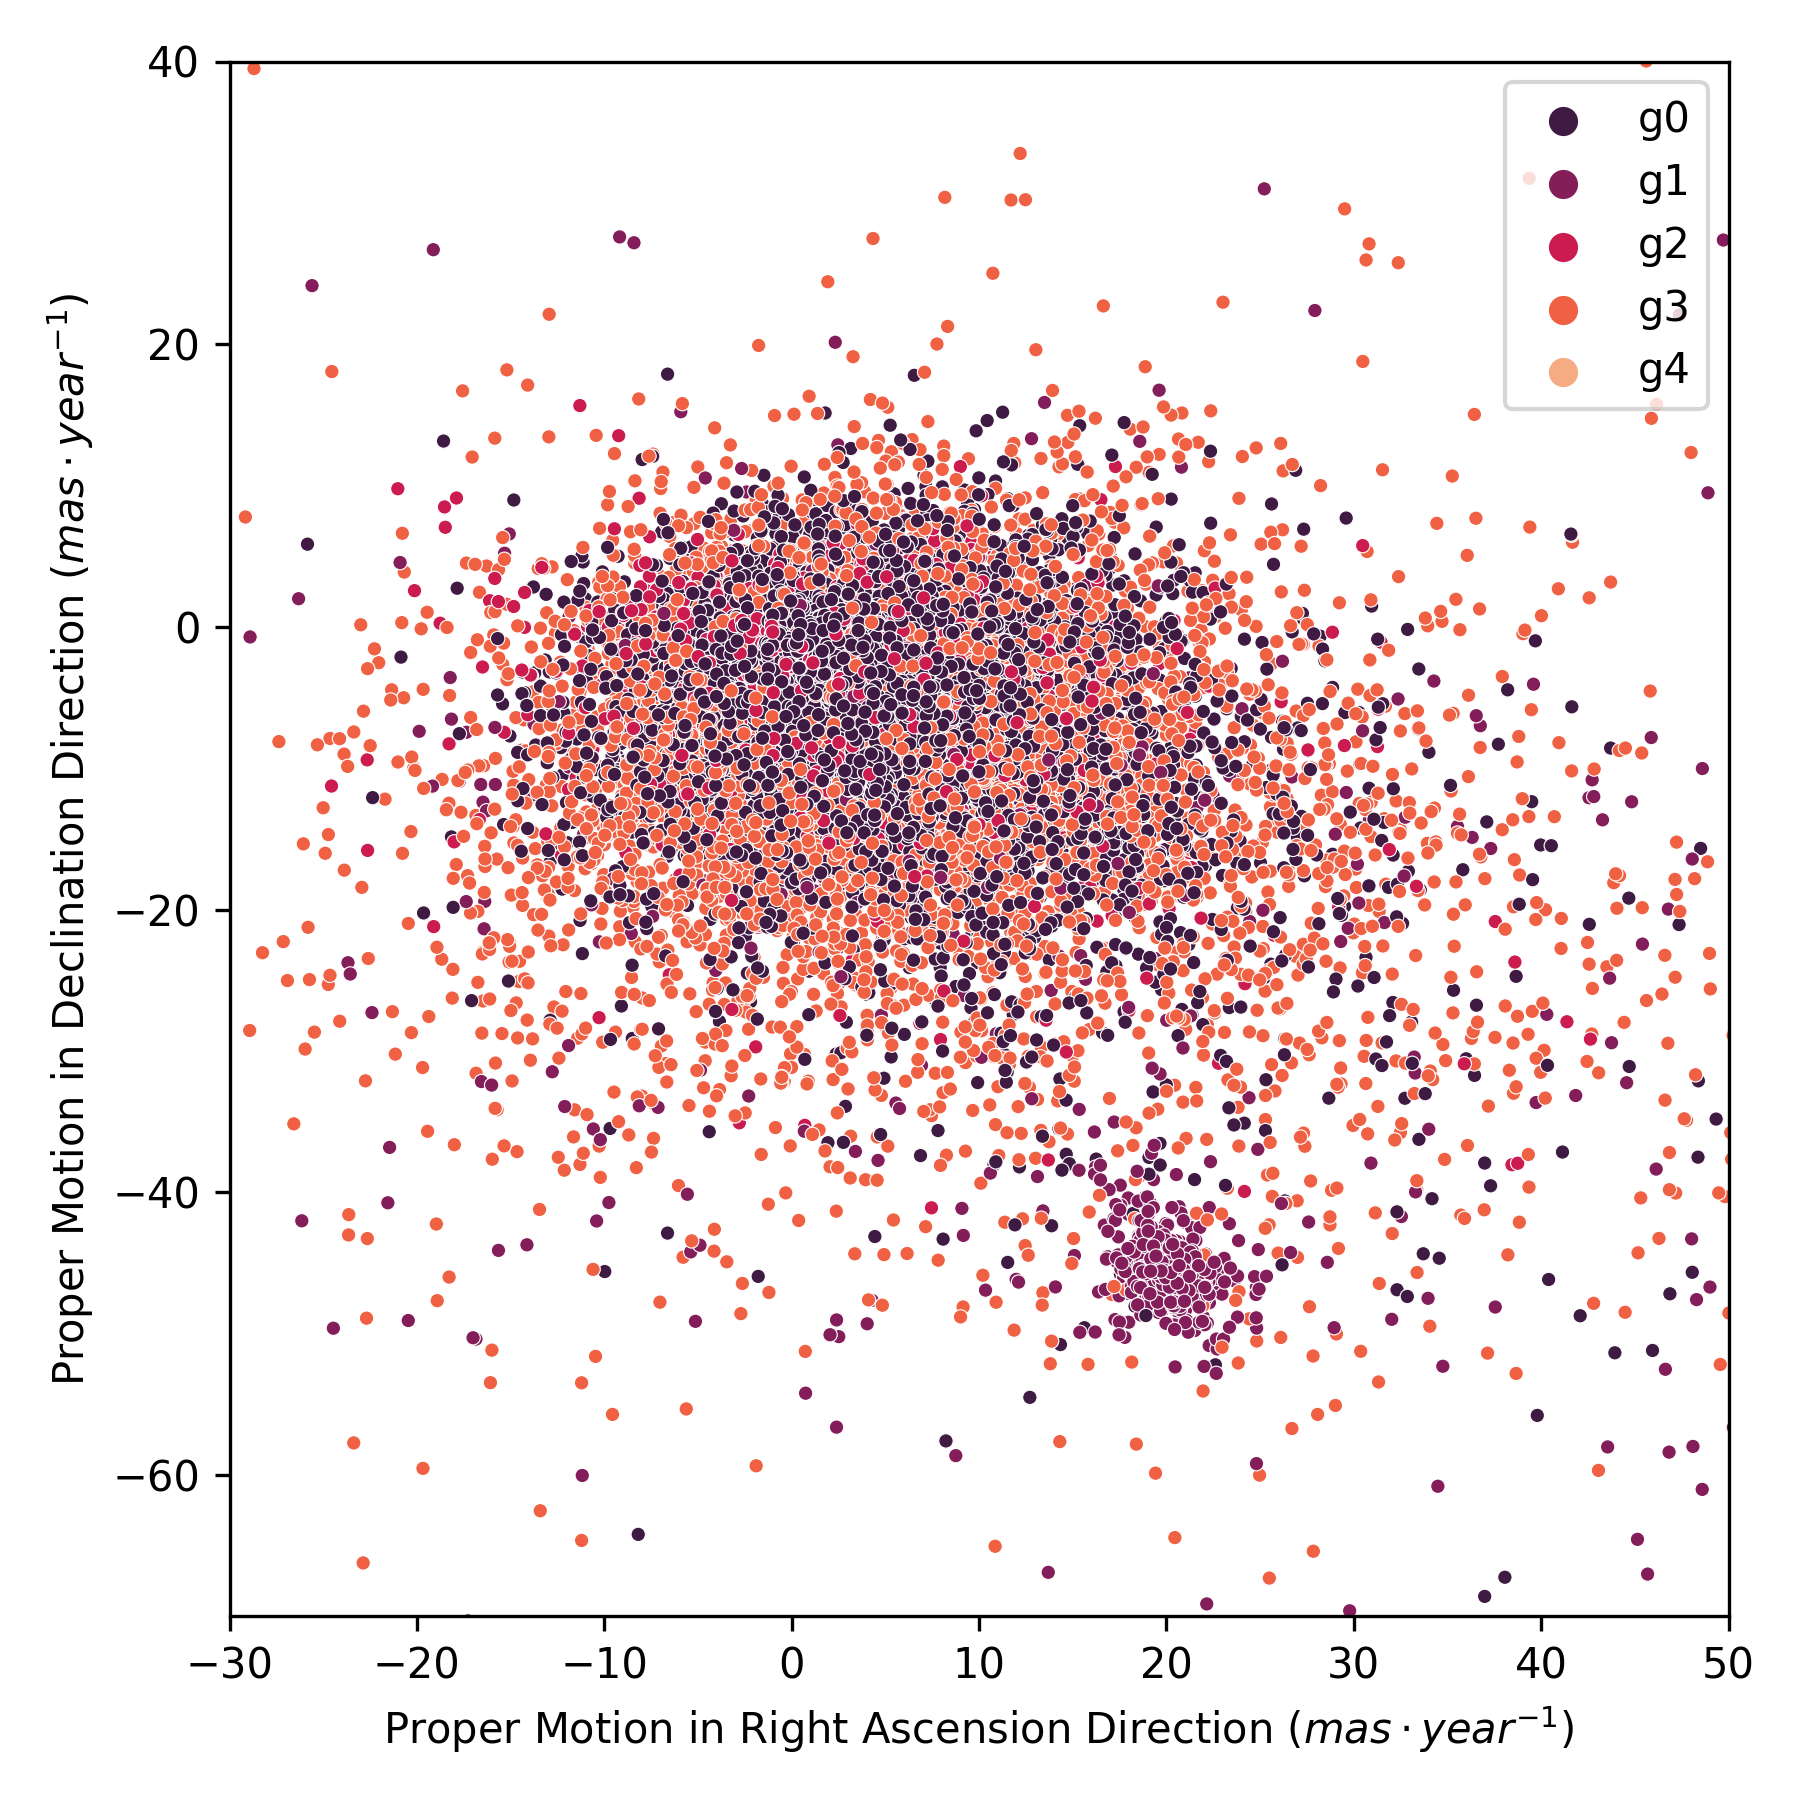
\includegraphics[width=\textwidth]{../figures/melotte_22/kmeans_pm_melotte_22.png}
    \end{subfigure}
    \hfill
    \begin{subfigure}[t]{0.3\textwidth}
      \centering
      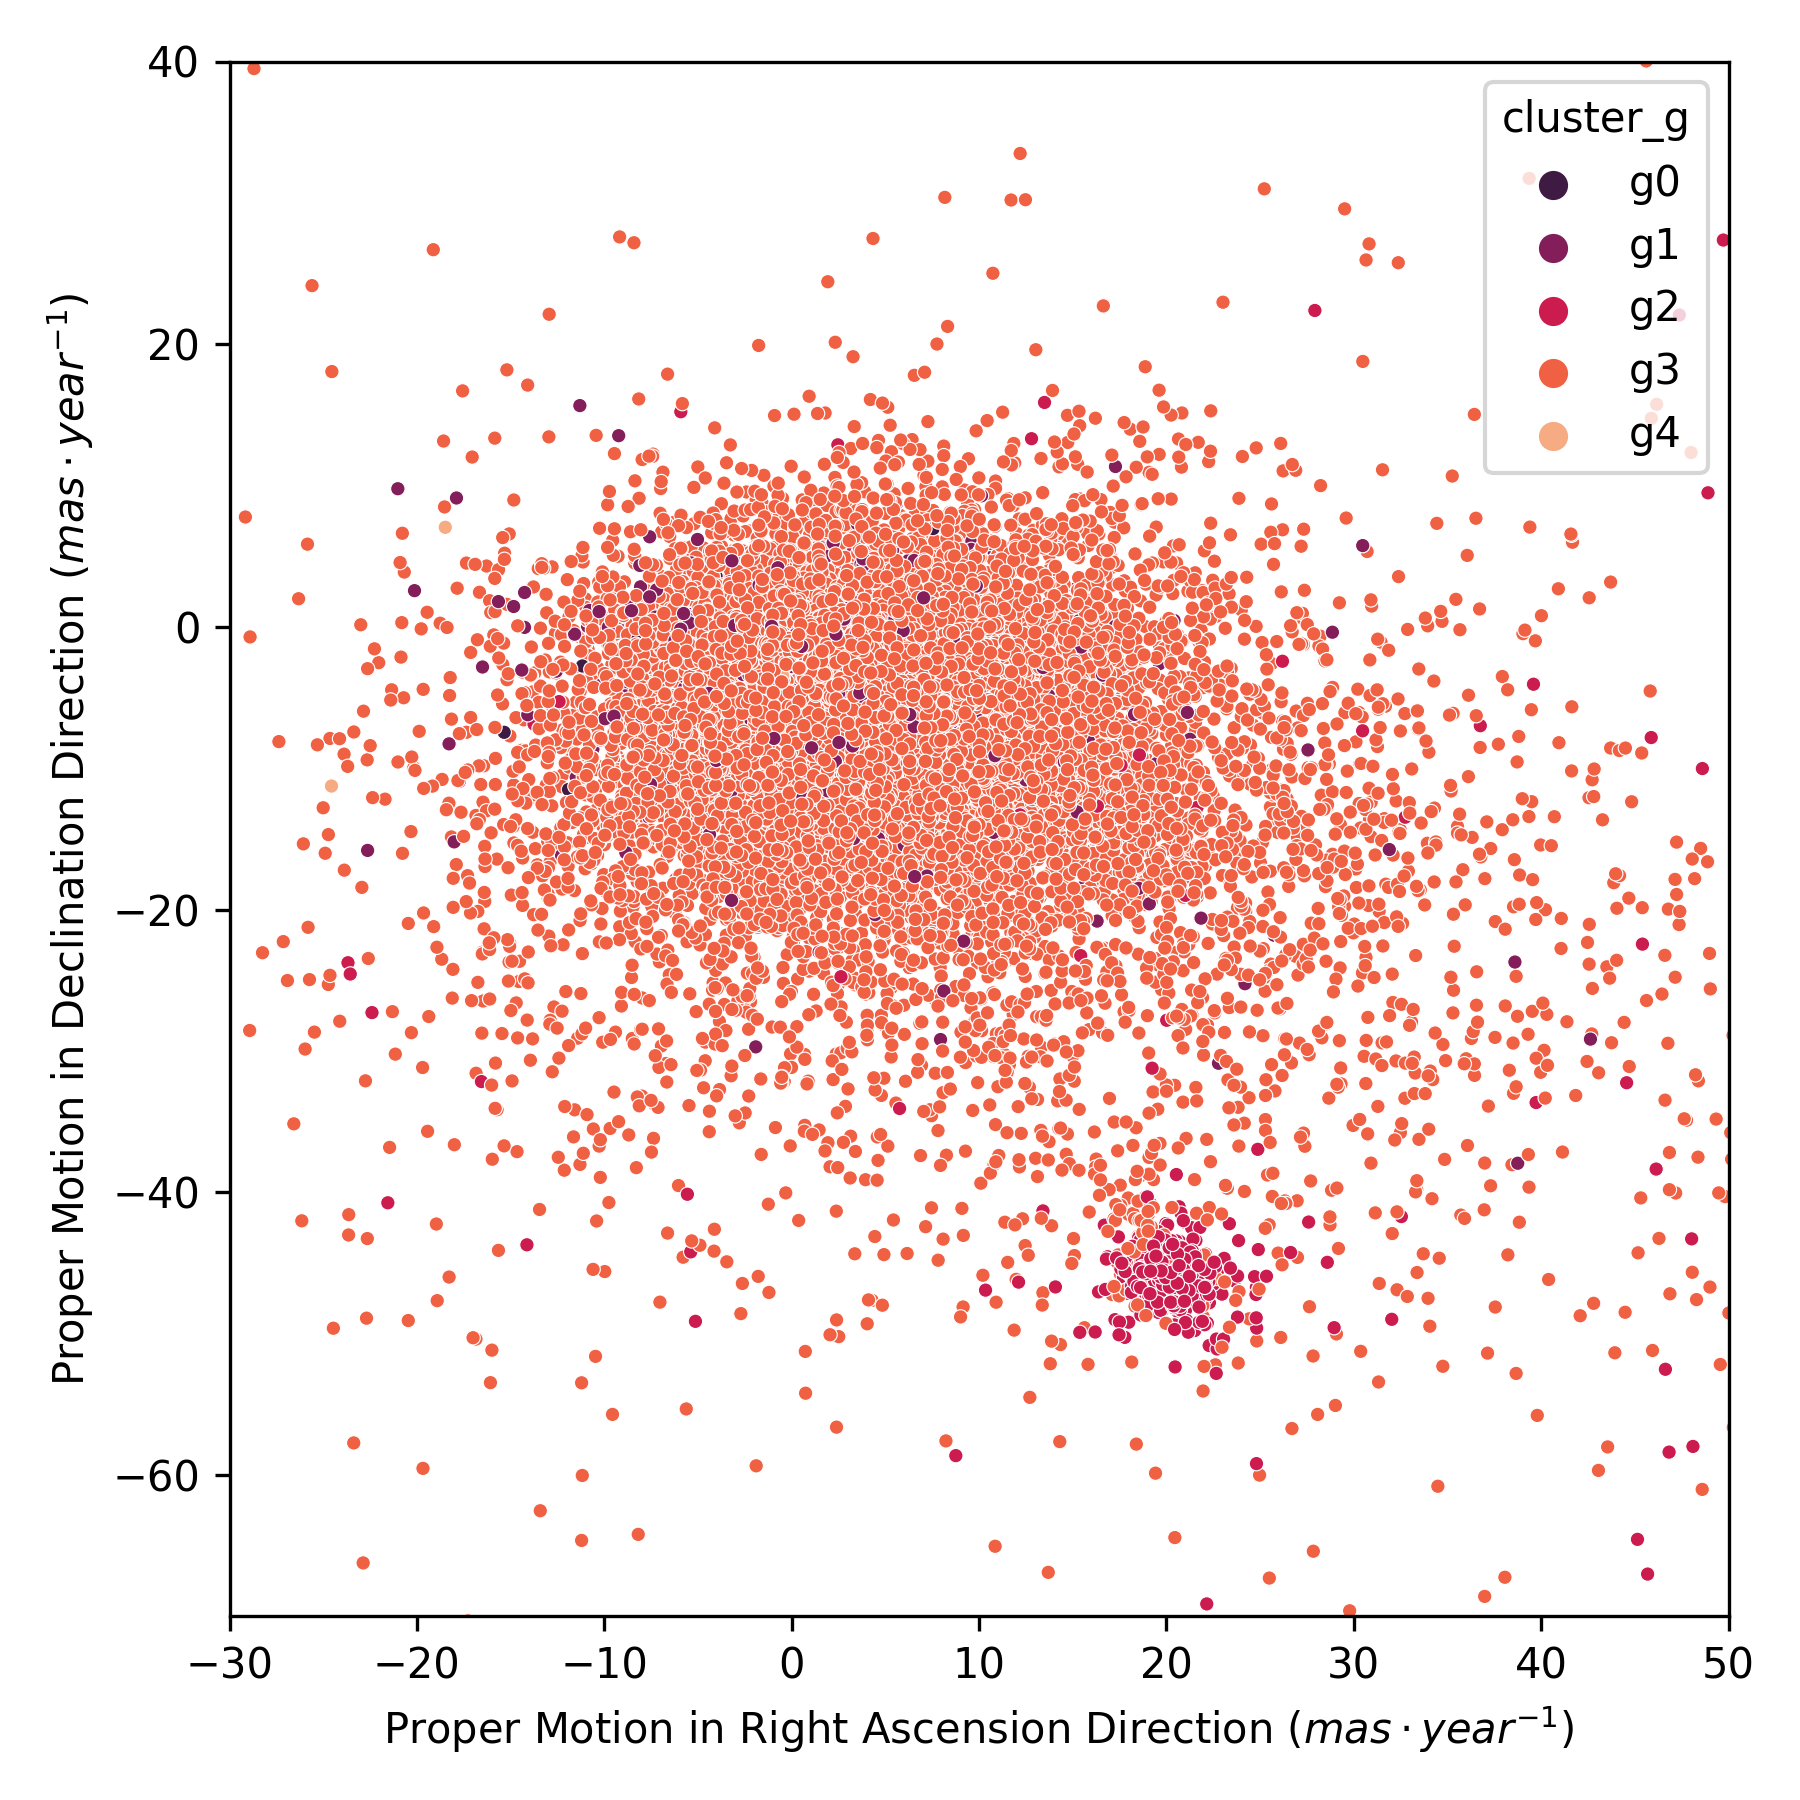
\includegraphics[width=\textwidth]{../figures/melotte_22/dec_pm_melotte_22.png}
    \end{subfigure}
    \hfill
    \begin{subfigure}[t]{0.3\textwidth}
      \centering
      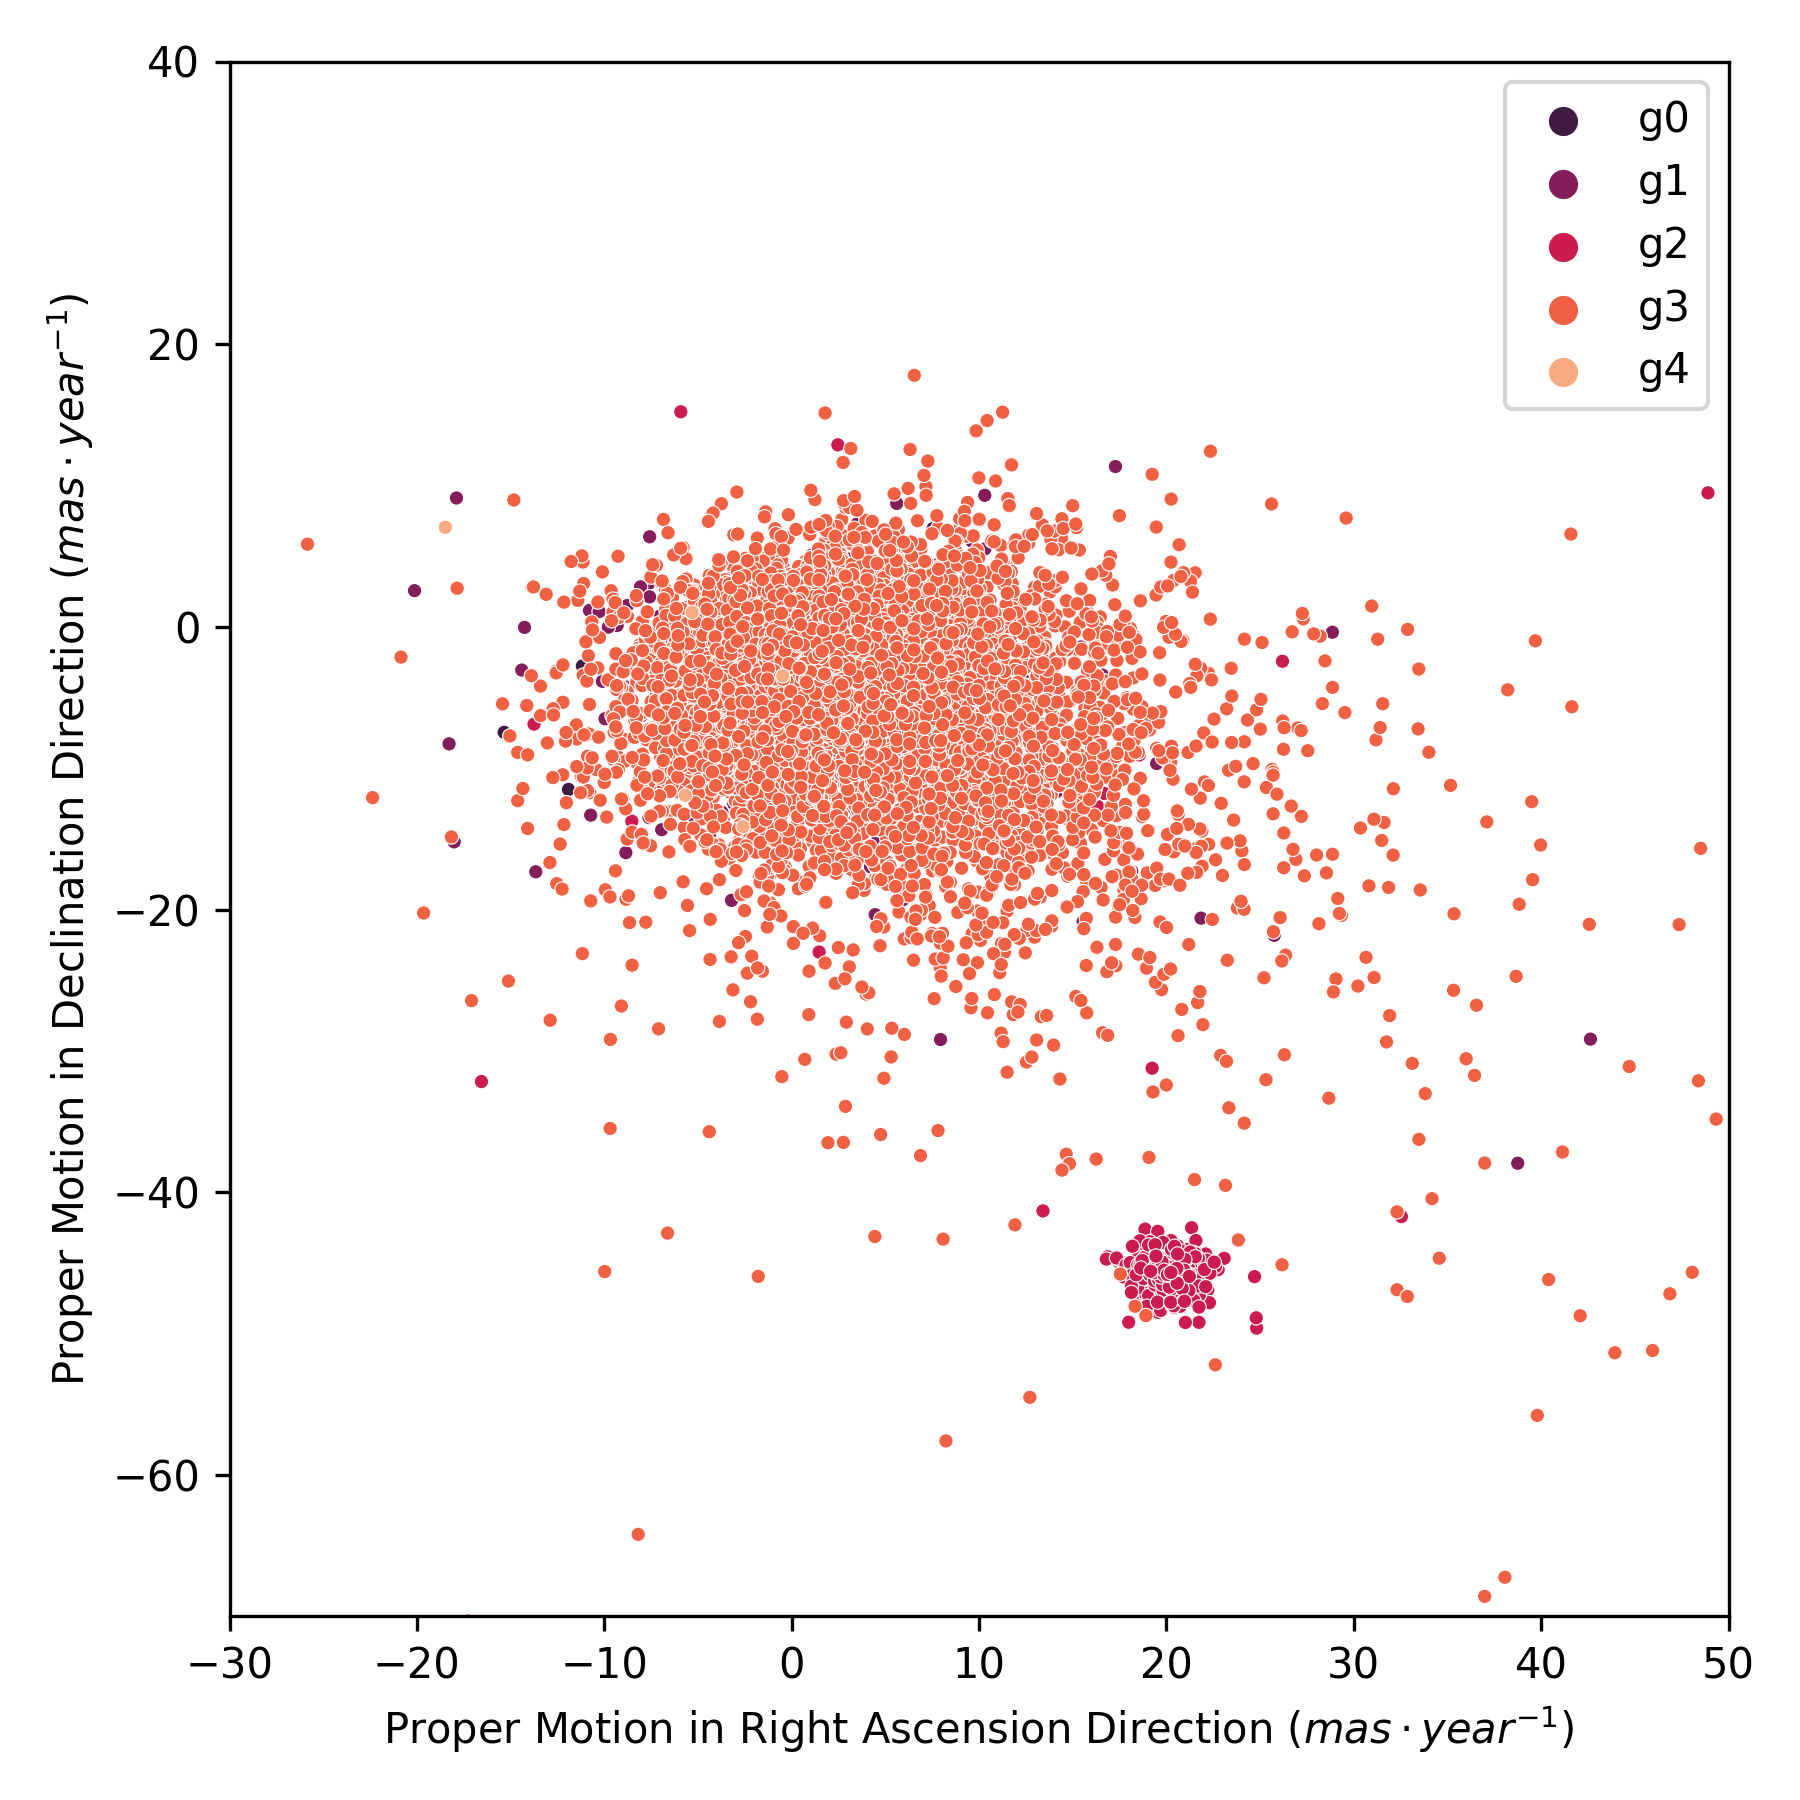
\includegraphics[width=\textwidth]{../figures/melotte_22/dec_pm_filtered_melotte_22.png}
    \end{subfigure}
  \end{subfigure}
  \medskip
  \begin{subfigure}{\columnwidth}
    \centering
    \begin{subfigure}[t]{0.3\textwidth}
      \centering
      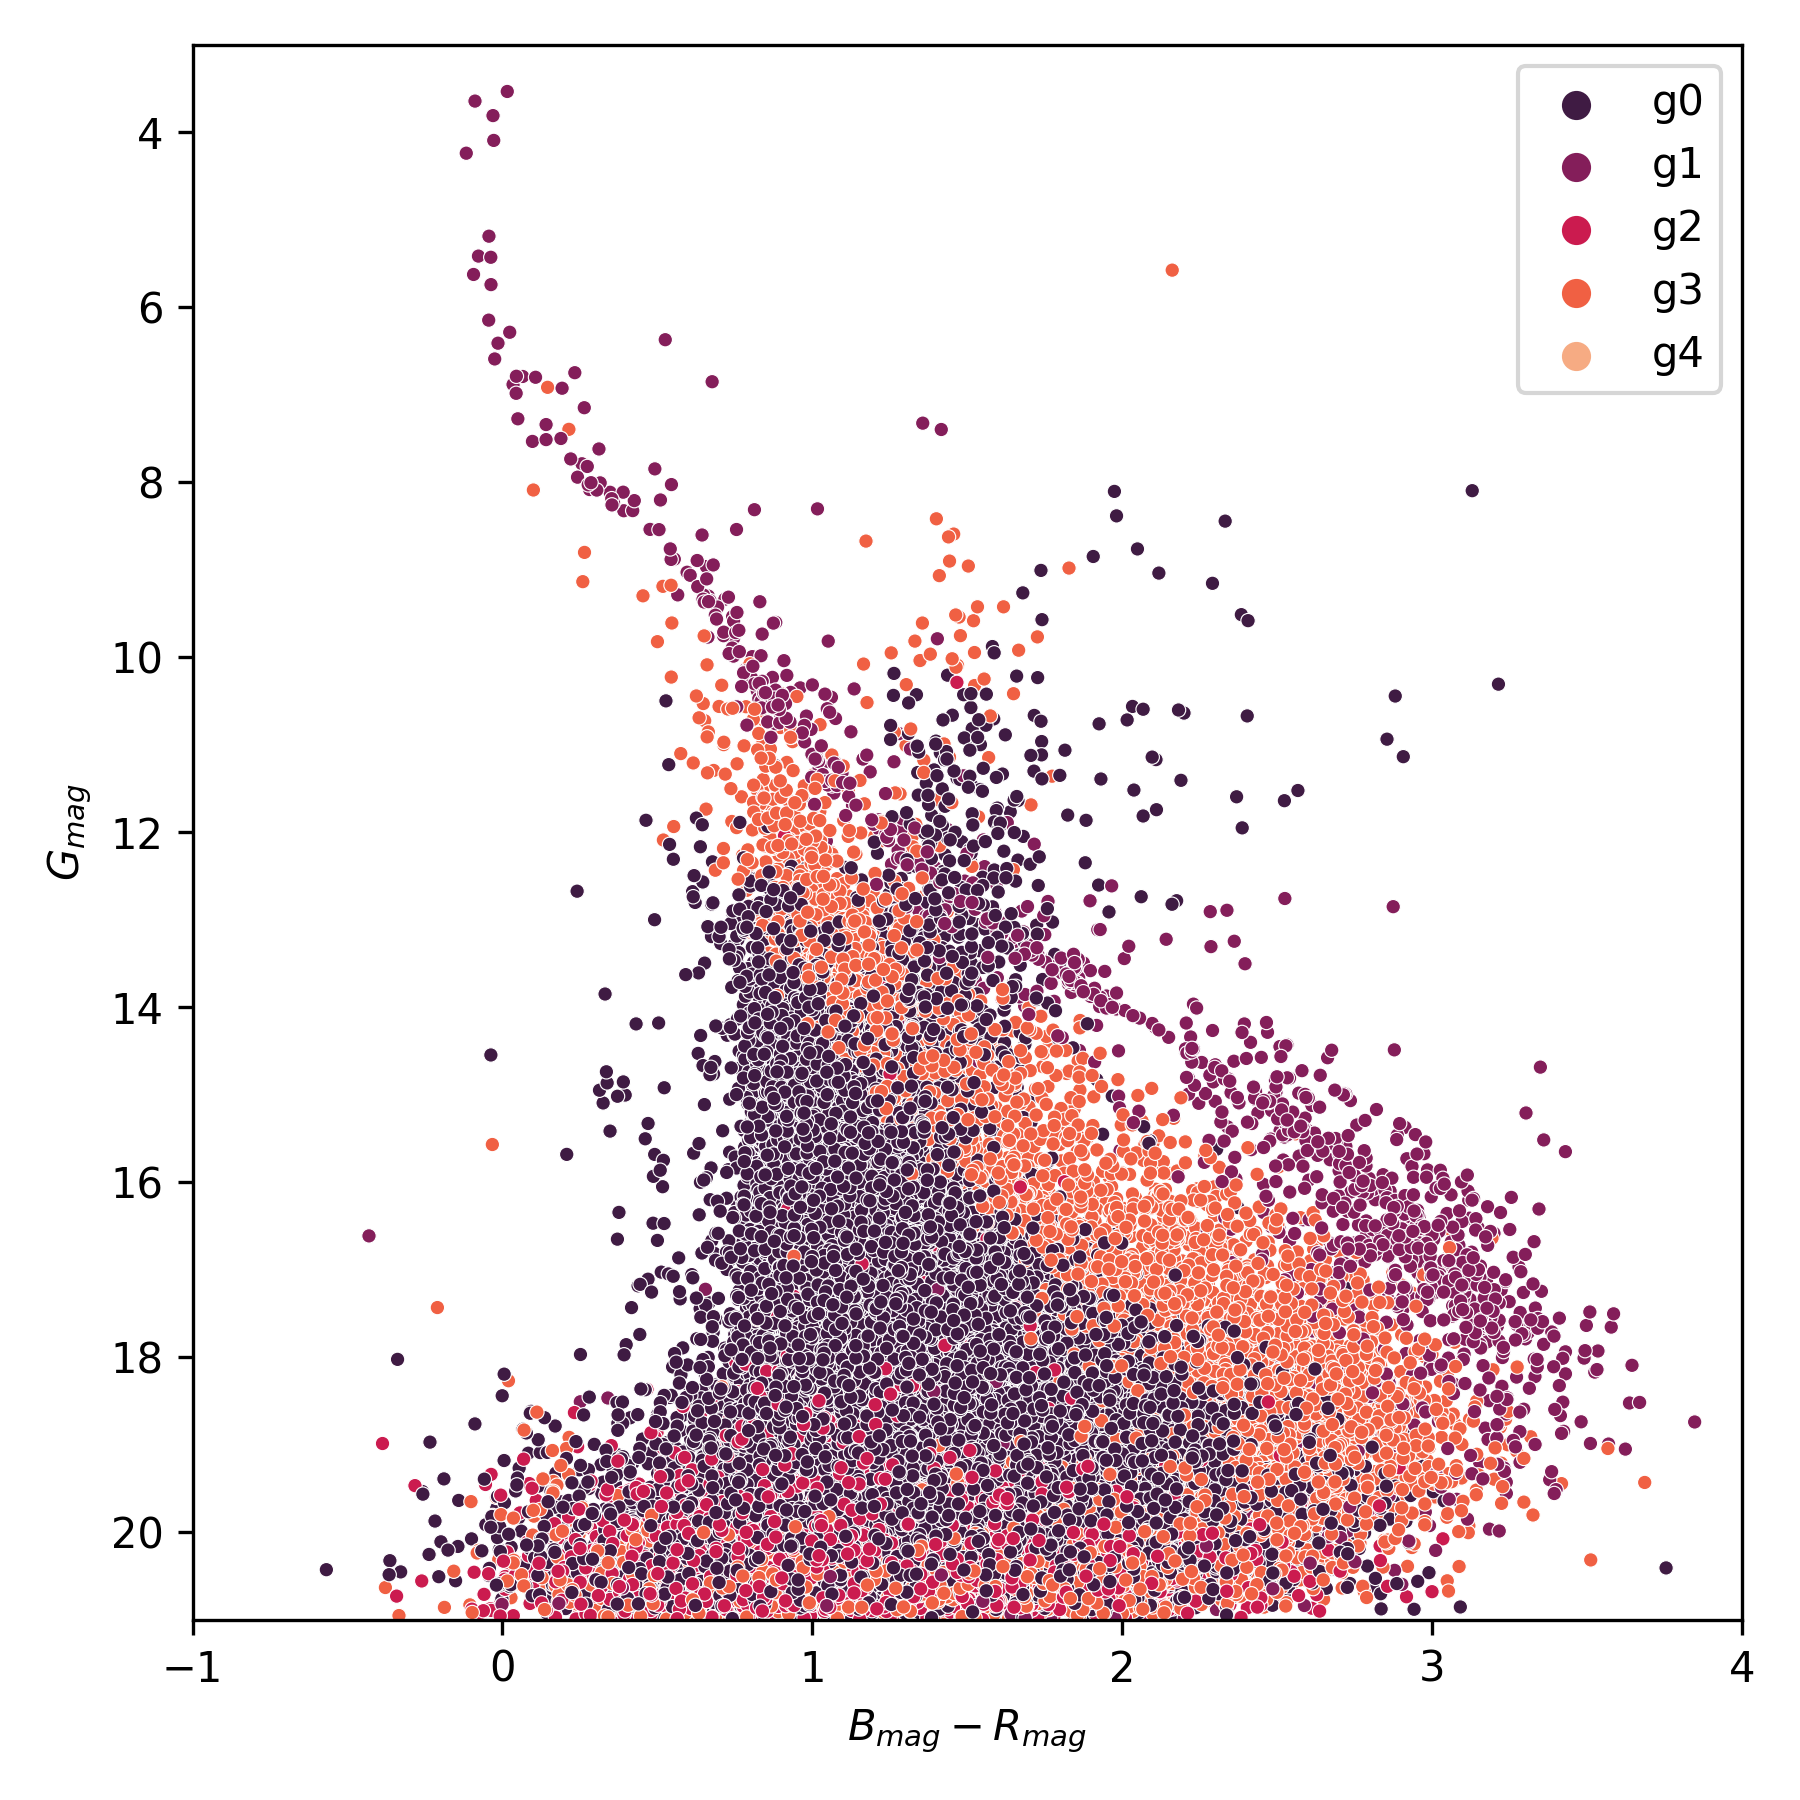
\includegraphics[width=\textwidth]{../figures/melotte_22/kmeans_hr_diagram_melotte_22.png}
      \caption{K-Means}
    \end{subfigure}
    \hfill
    \begin{subfigure}[t]{0.3\textwidth}
      \centering
      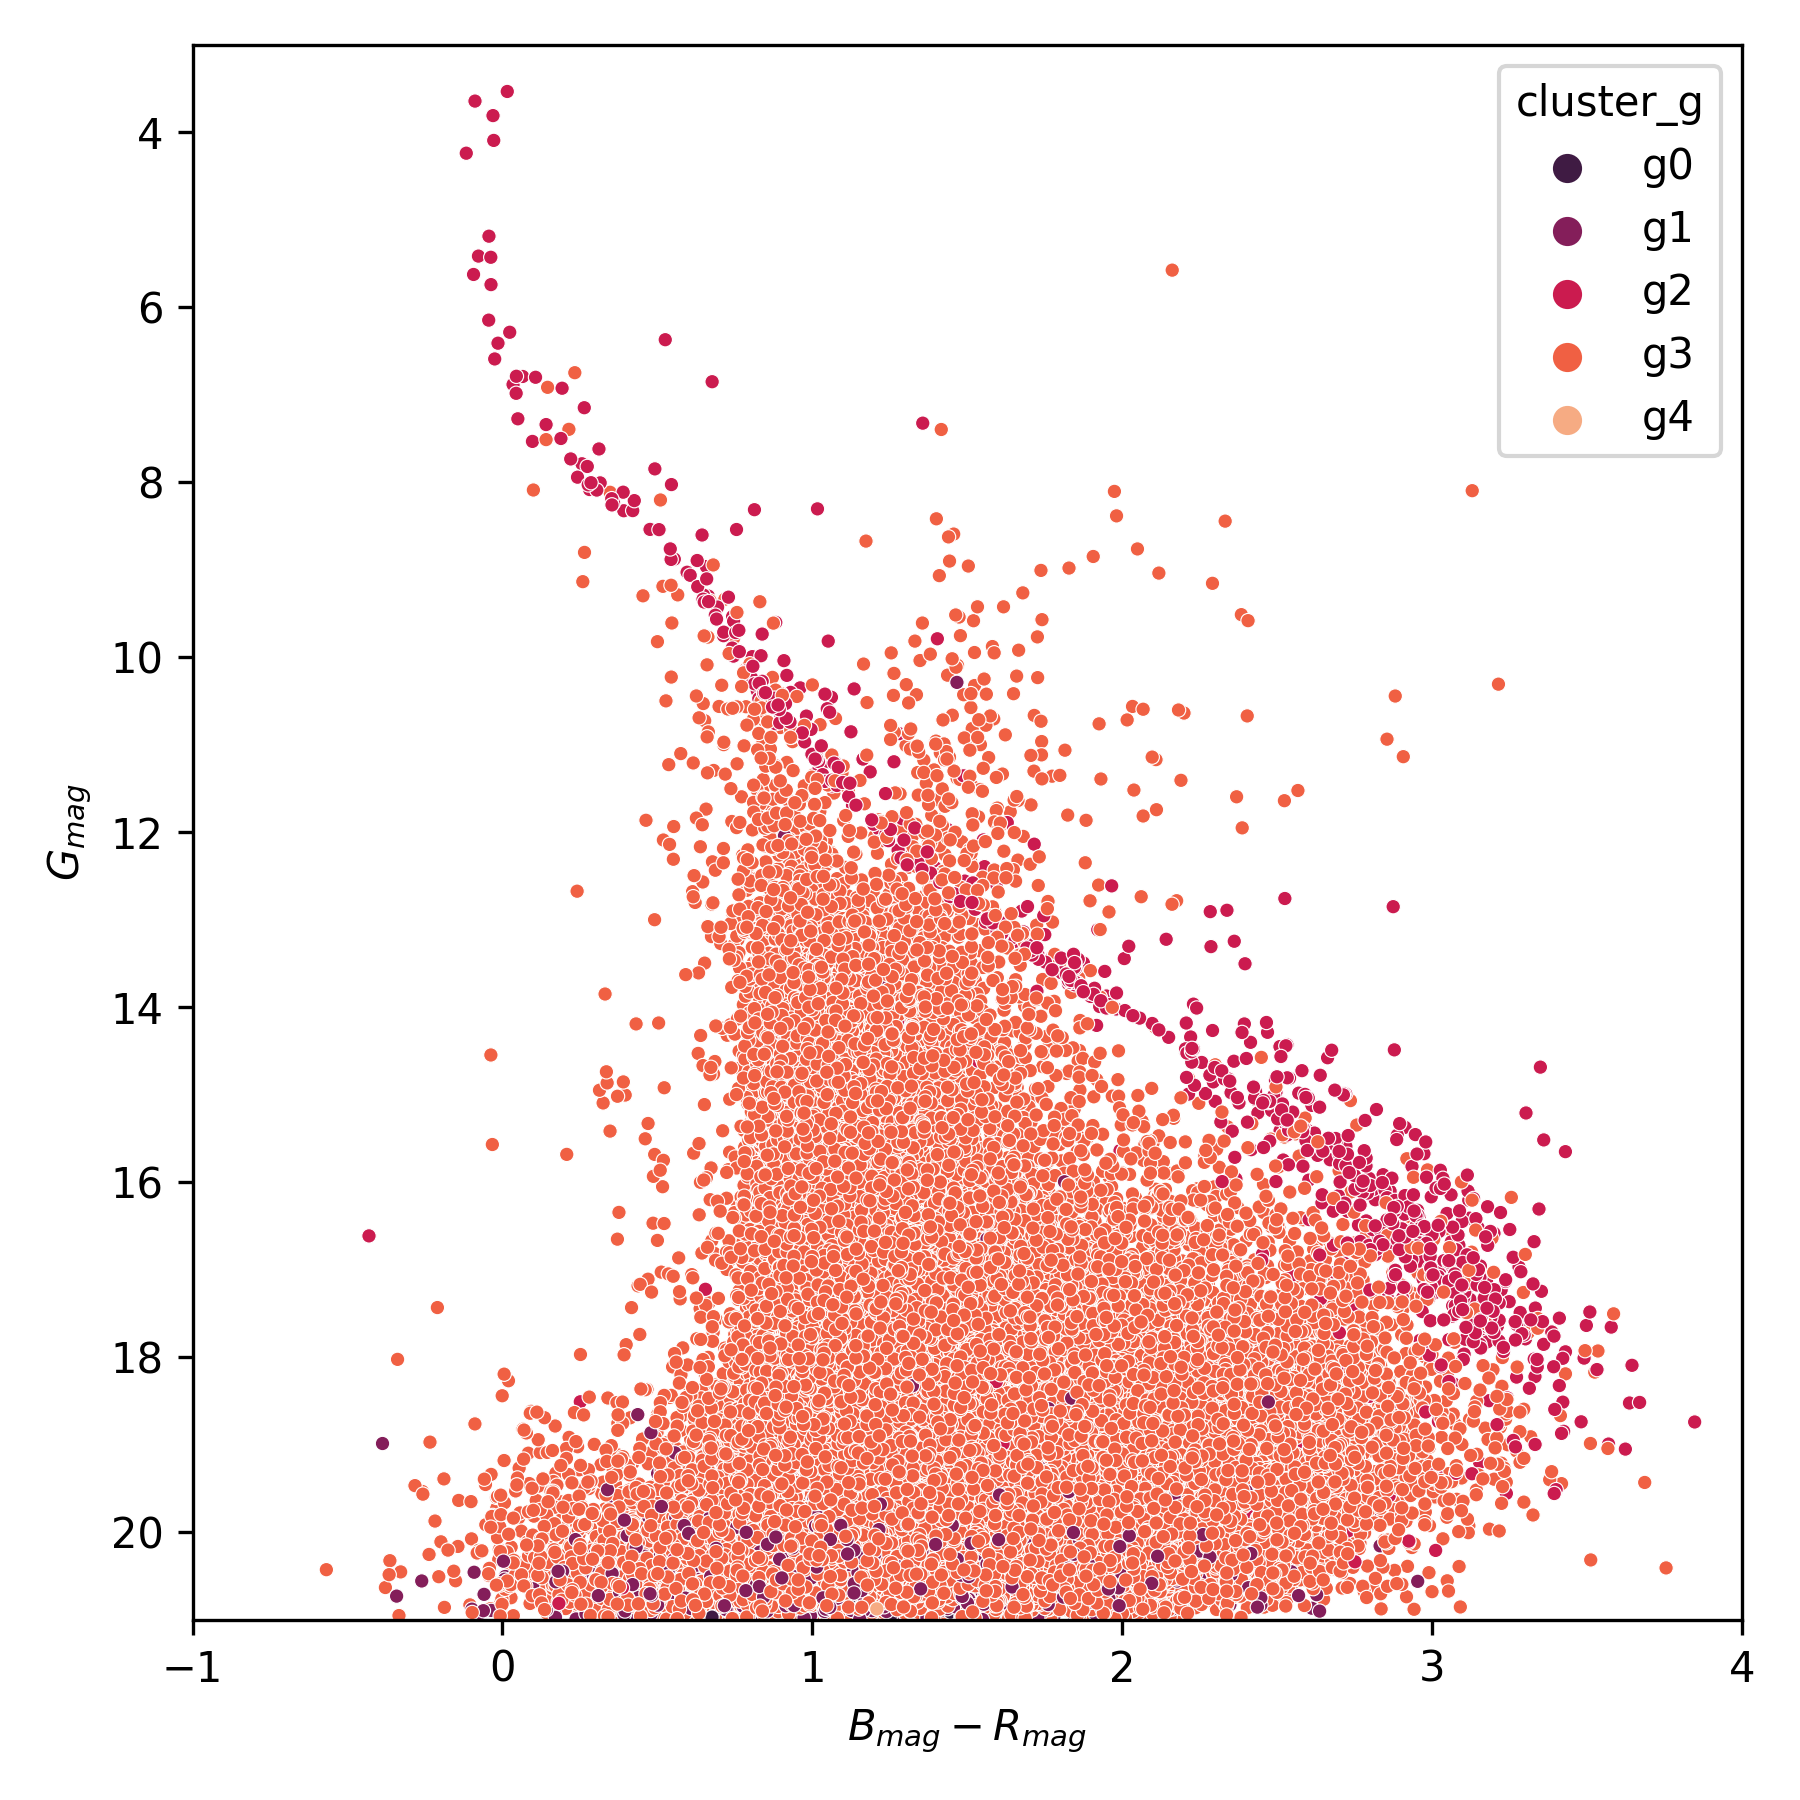
\includegraphics[width=\textwidth]{../figures/melotte_22/dec_hr_diagram_melotte_22.png}
      \caption{DEC}
    \end{subfigure}
    \hfill
    \begin{subfigure}[t]{0.3\textwidth}
      \centering
      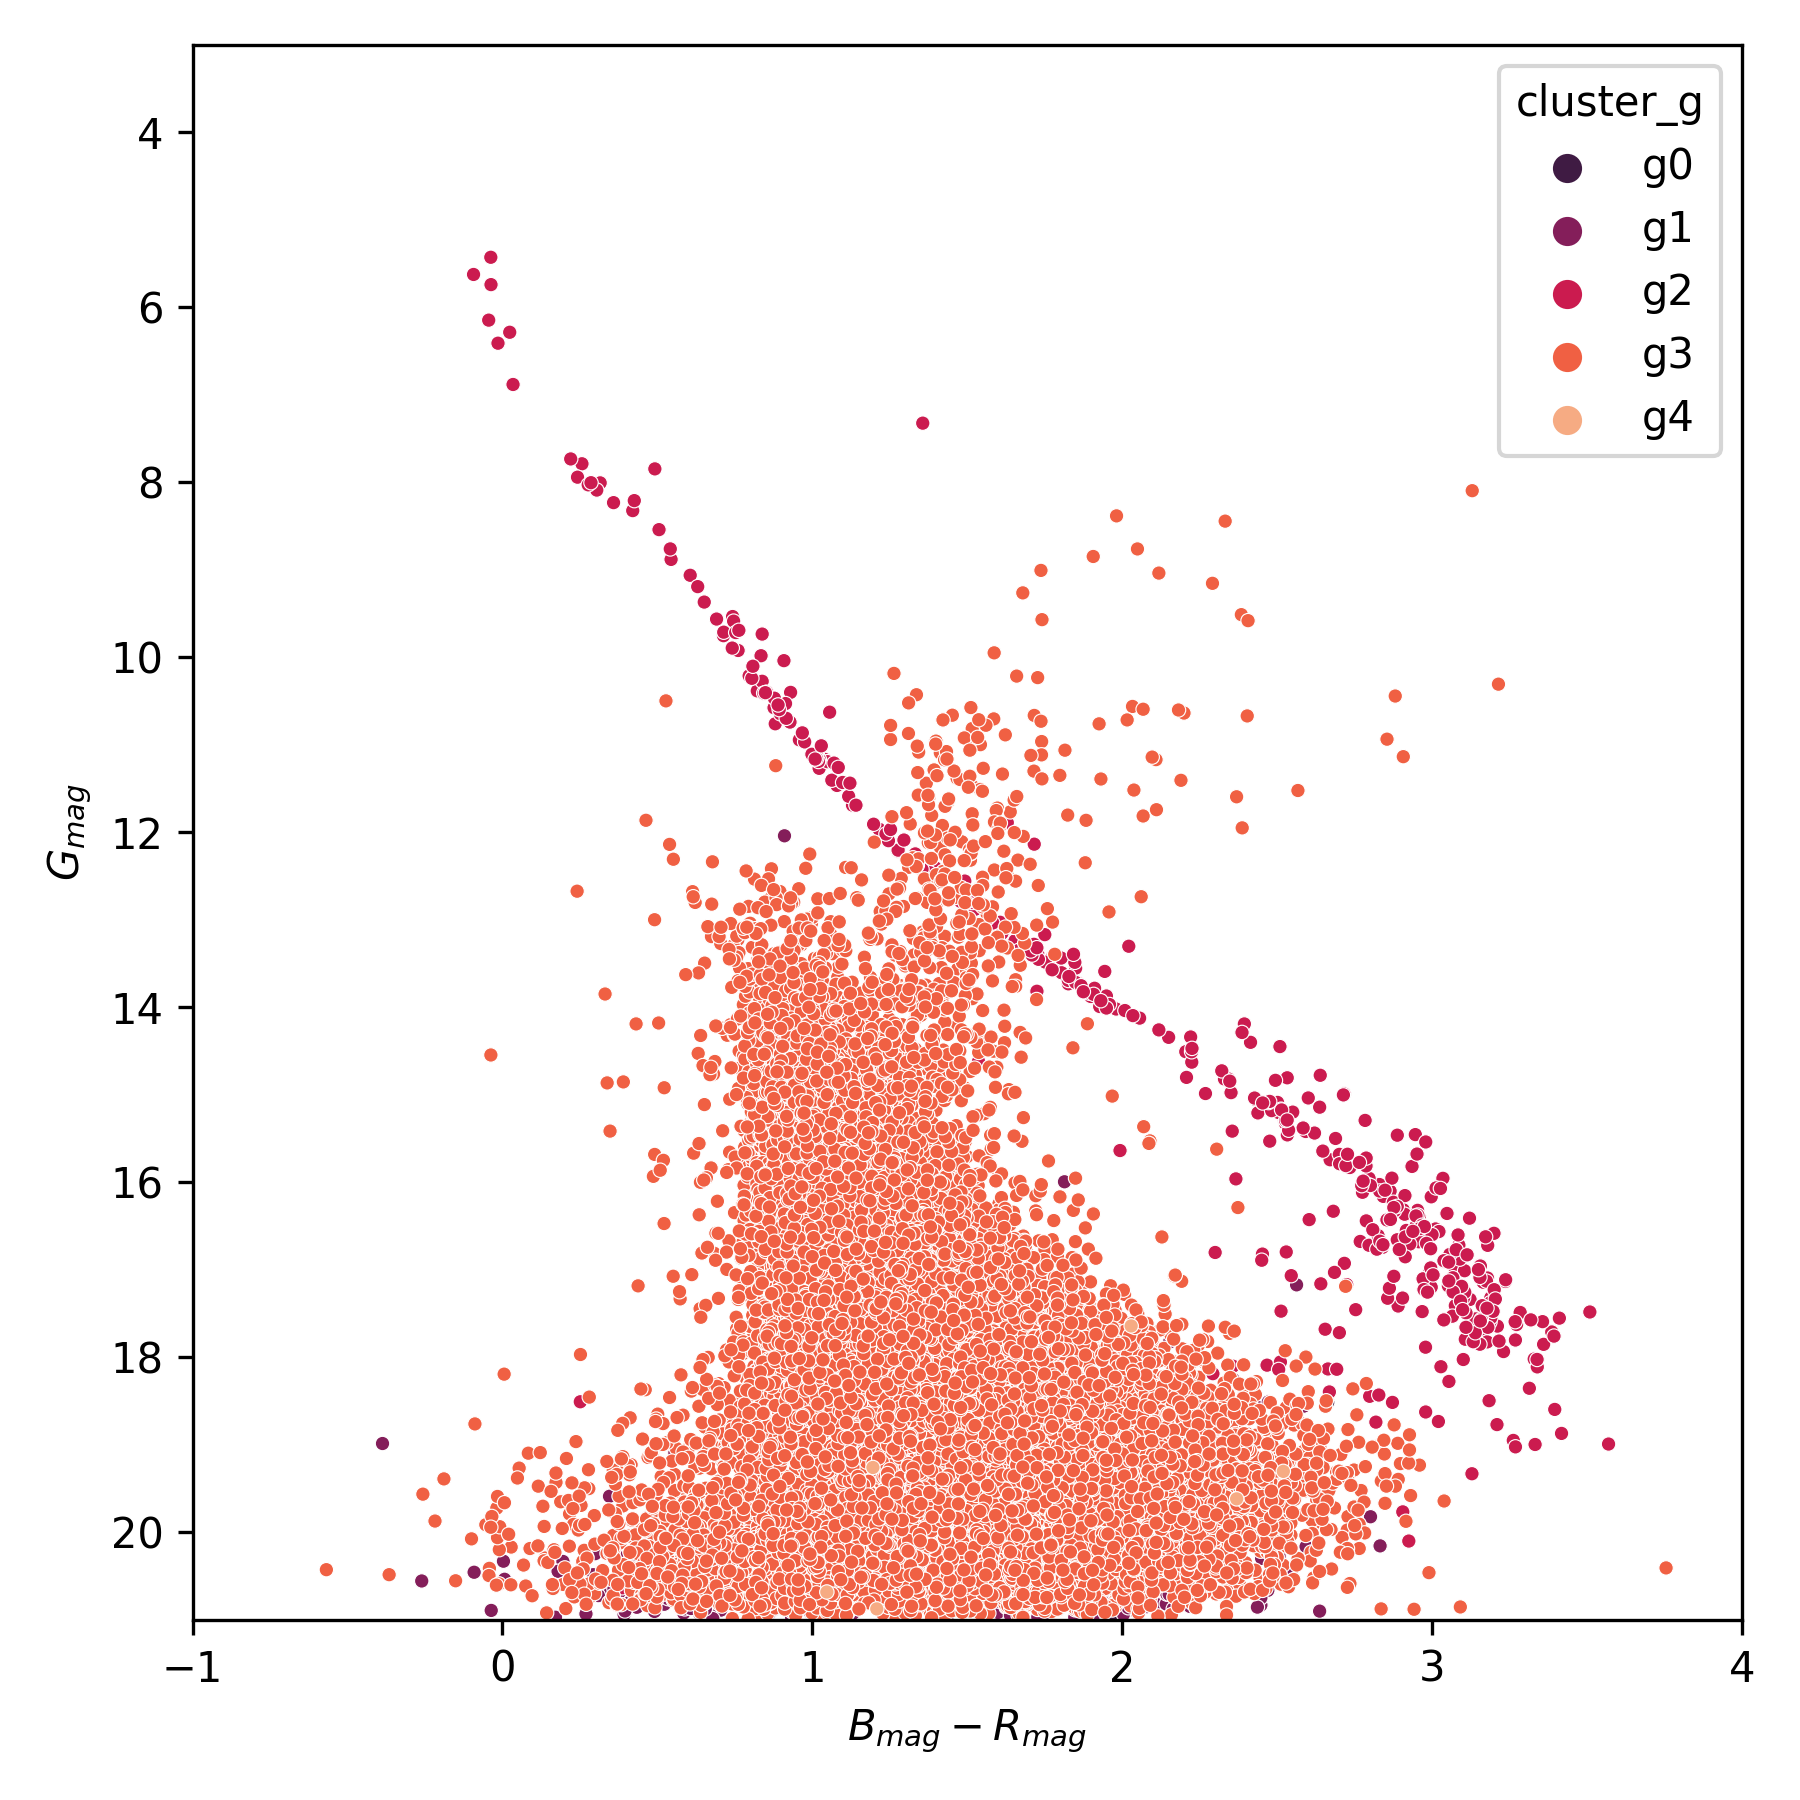
\includegraphics[width=\textwidth]{../figures/melotte_22/dec_hr_diagram_filtered_melotte_22.png}
      \caption{DEC (filt.)}
    \end{subfigure}
  \end{subfigure}
  \caption{Evolution of Melotte 22 characterization}
  \label{fig:melotte_22_characterization_evolution}
\end{figure}

Figure \ref{fig:melotte_22_characterization_evolution} shows the evolution
of the characterization of Melotte 22. The first column corresponds to the
characterization obtained by applying K-Means alone to the dataset. The middle
column is the characterization made by the DEC model. And the column on the right
shows the characterization made by the DEC and having filtered the quantiles
lower than 0.10 and higher than 0.90. The top row shows the proper motion
configuration space while the bottom one shows the Hertzsprung–Russell diagrams.

All resources developed for this project are available at the GitHub repository:
\href{https://github.com/cdalvaro/machine-learning-master-thesis}{cdalvaro/machine-learning-master-thesis}

It includes the DEC model developed in Python using the Keras framework
and Jupyter Notebooks \cite{Kluyver2016jupyter} with examples.

\section{CONTRIBUTION}

The developed method is successful since it meets all our established requirements:

\begin{itemize}
  \item Our method gives valid results compatible with current methods as described in Section \ref{sec:results}.
  \item As required from the beginning, it is non-supervised and non-parameterized.
  \item The model shows a great performance compared with current methods.
  \item It is able to deal with large and open regions. As an example,
        it has succeeded characterizing Melotte 25 (Hiades) OC. Also,
        the relative proximity of this cluster, 45 parsec, makes it difficult to
        characterize. Clusterix fails characterizing this cluster. In this case,
        our method proposes at least two more non-catalogued clusters. The analysis
        of these new clusters brings out an interesting stellar dynamics in the studied
        region. It could mean that there was a recent interaction among different molecular clouds.
\end{itemize}

For all this, we consider that the presented method is good enough to be included
in the Virtual Observatory toolset. Only a few tweaks must be done in order to make
our model compatible with other tools of the VO.

\section{RESULTS}
\label{sec:results}

We now present the results obtained after having analyzed Melotte 25.
This is the largest cluster we have studied and one of the most difficult
to characterize by its distribution and extension.

More results are available at Appendix \ref{sec:appendix}.

Melotte 25 is located at 66.725 degrees in right ascension and 15.867
degrees in declination with a radius of 165 arcmin.
This region contains more than 400,000 stars.

Table \ref{tab:results_melotte_25} shows a results summary for Melotte 25.

\begin{table}[htbp]
  \begin{center}
    \resizebox{\columnwidth}{!}{
      \begin{tabular}{l|c|c|c|c}
        \textbf{Method} & \emph{$\mu_{\alpha}$ $(mas/yr^{-1})$} & \emph{$\mu_{\delta}$ $(mas/yr^{-1})$} & \emph{$\varpi$ $(mas)$} & \emph{\# stars} \\
        \hline
        \textbf{Simbad}\tablefootnote{Results have been taken from the SIMBAD astronomical database\cite{wenger2000simbad}} & 104.92 $\pm$ 0.12 & -28.00 $\pm$ 0.09 & 21.052 $\pm$ 0.065 & - \\
        Clusterix & 106.796 $\pm$ 6.229 & -24.870 $\pm$ 5.417 & 21.210 $\pm$ 1.115 & 109 \\
        K-Means & 79.936 $\pm$ 3.7 & -45.362 $\pm$ 3.8 & 20.901 $\pm$ 0.31 & 374 \\
        DEC & 104.051 $\pm$ 3.2 & -33.424 $\pm$ 2.5 & 22.072 $\pm$ 0.13 & 219 \\
        \textbf{DEC (filt.)} & 105.96 $\pm$ 3.5 & -30.00 $\pm$ 2.4 & 21.74 $\pm$ 0.07 & 175 \\
      \end{tabular}
    }
    \caption{Melotte 25 results.}
    \label{tab:results_melotte_25}
  \end{center}
\end{table}

Parameters shown are proper motion in right ascension and declination, parallax
with their respective deviations and number of stars corresponding to the OC.

Figure \ref{fig:result_melotte_25_dec} shows the groups found using the DEC model.
This model labels Melotte 25 as group \emph{g5}.

\begin{figure}[htbp]
  \centering
  \begin{subfigure}{\columnwidth}
    \centering
    \begin{subfigure}[t]{0.30\textwidth}
      \centering
      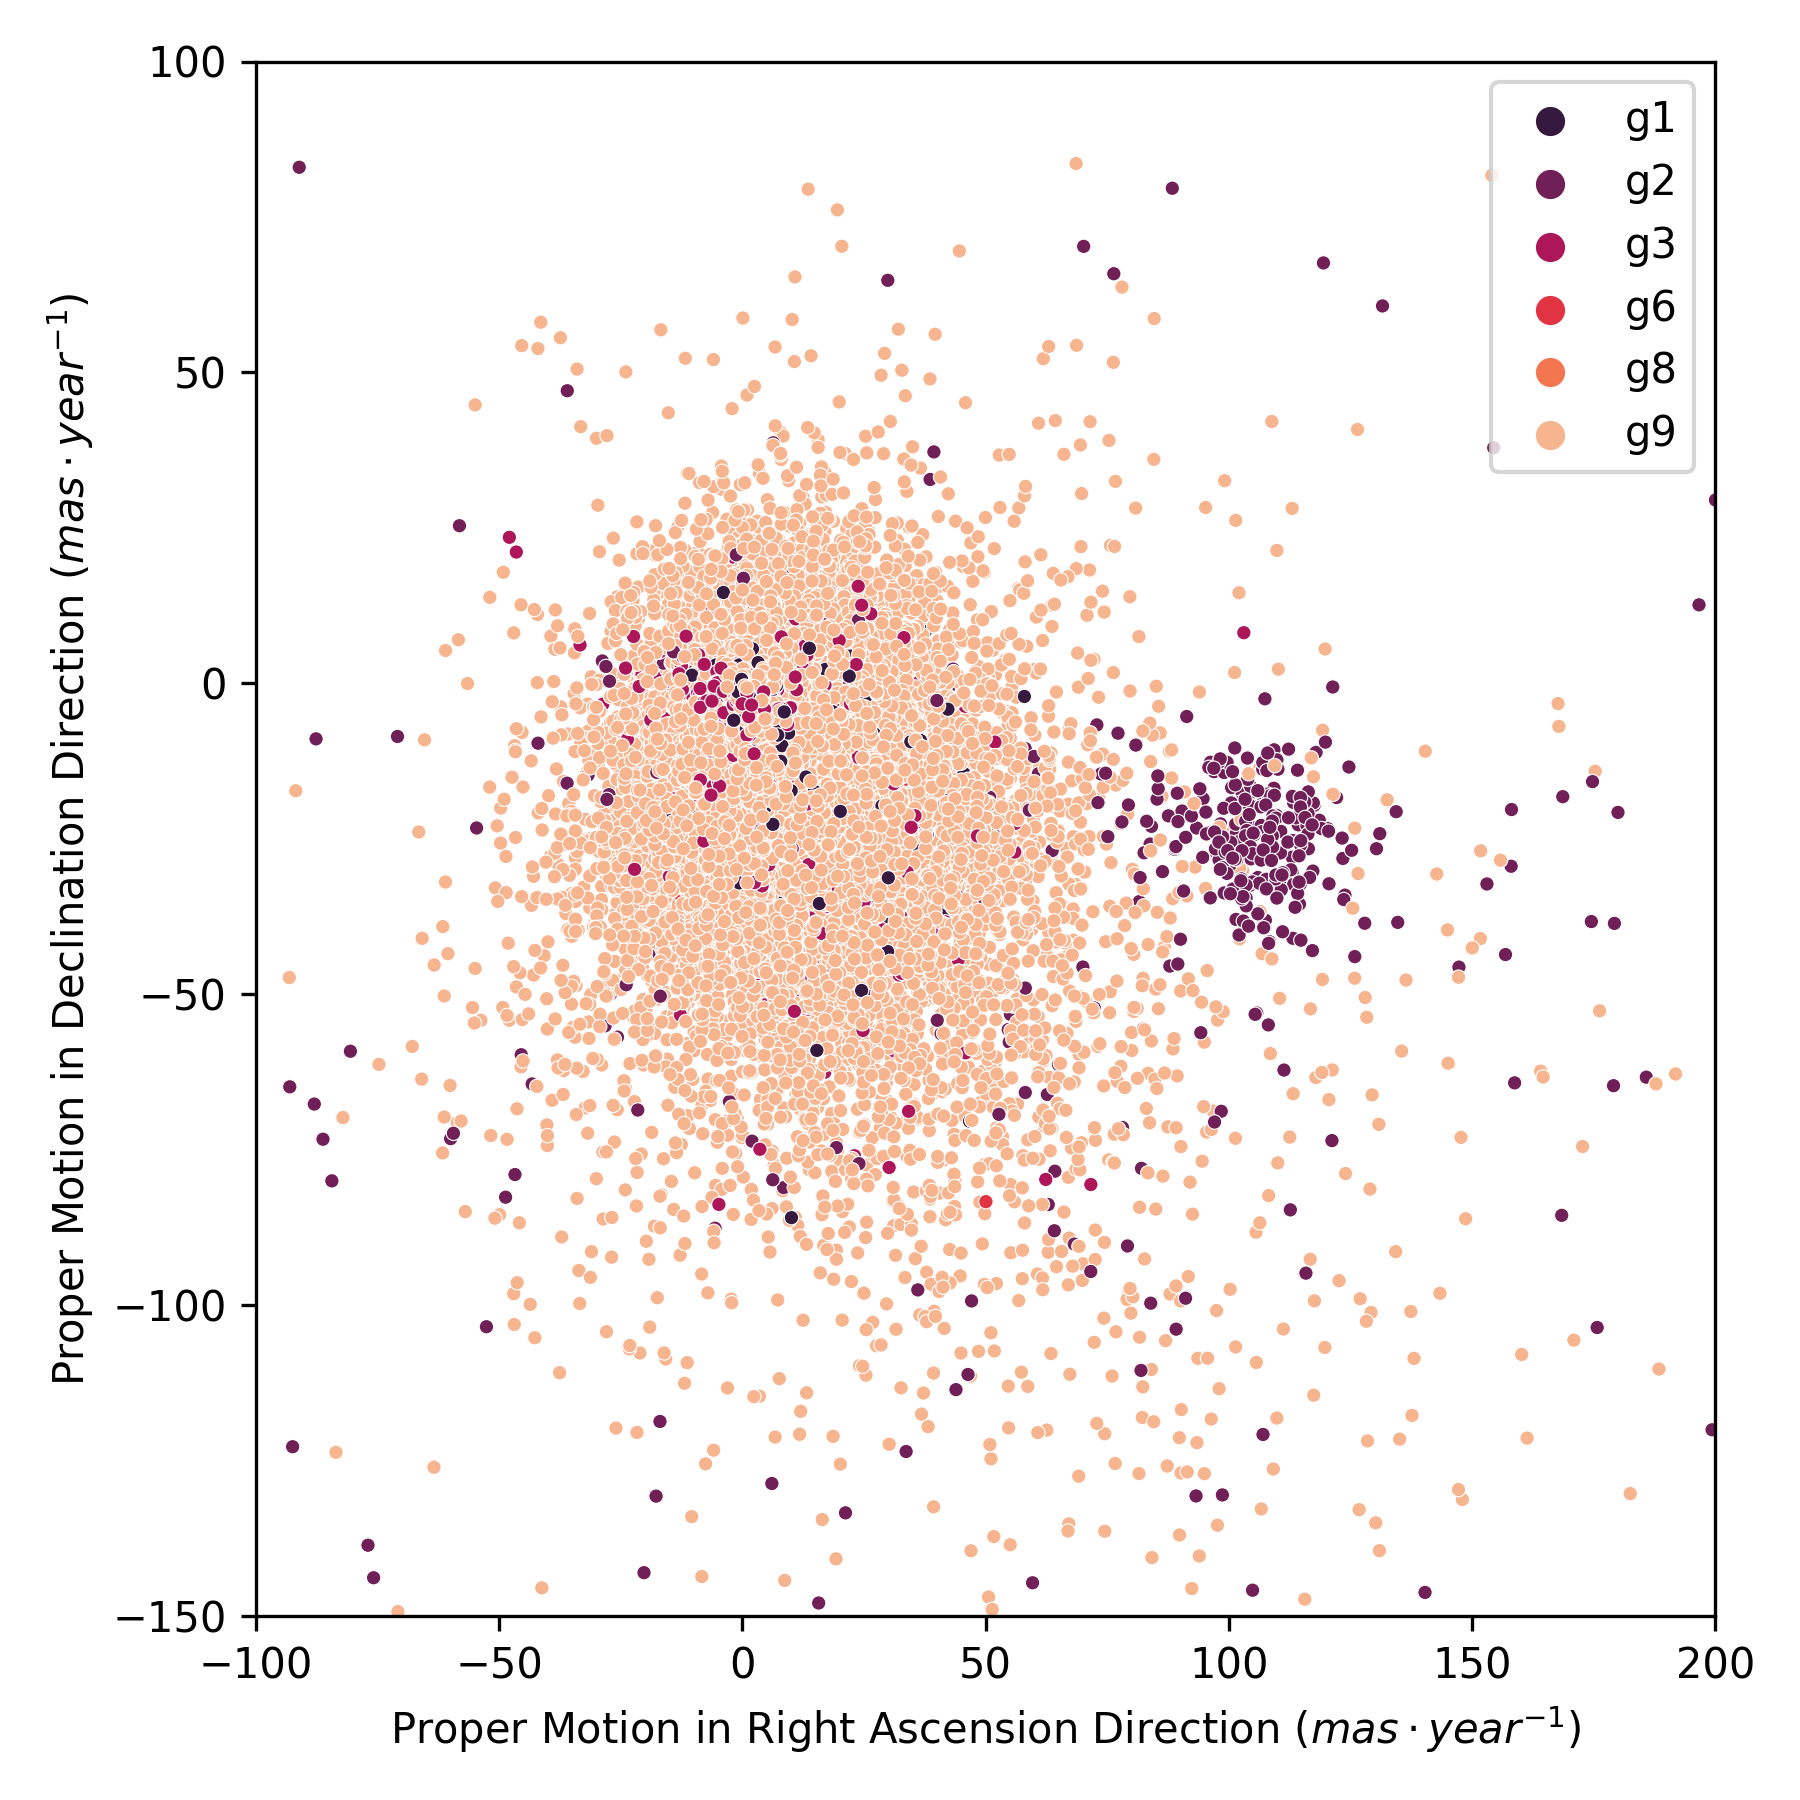
\includegraphics[width=\textwidth]{../figures/melotte_25/dec_pm_melotte_25.png}
    \end{subfigure}
    \hfill
    \begin{subfigure}[t]{0.30\textwidth}
      \centering
      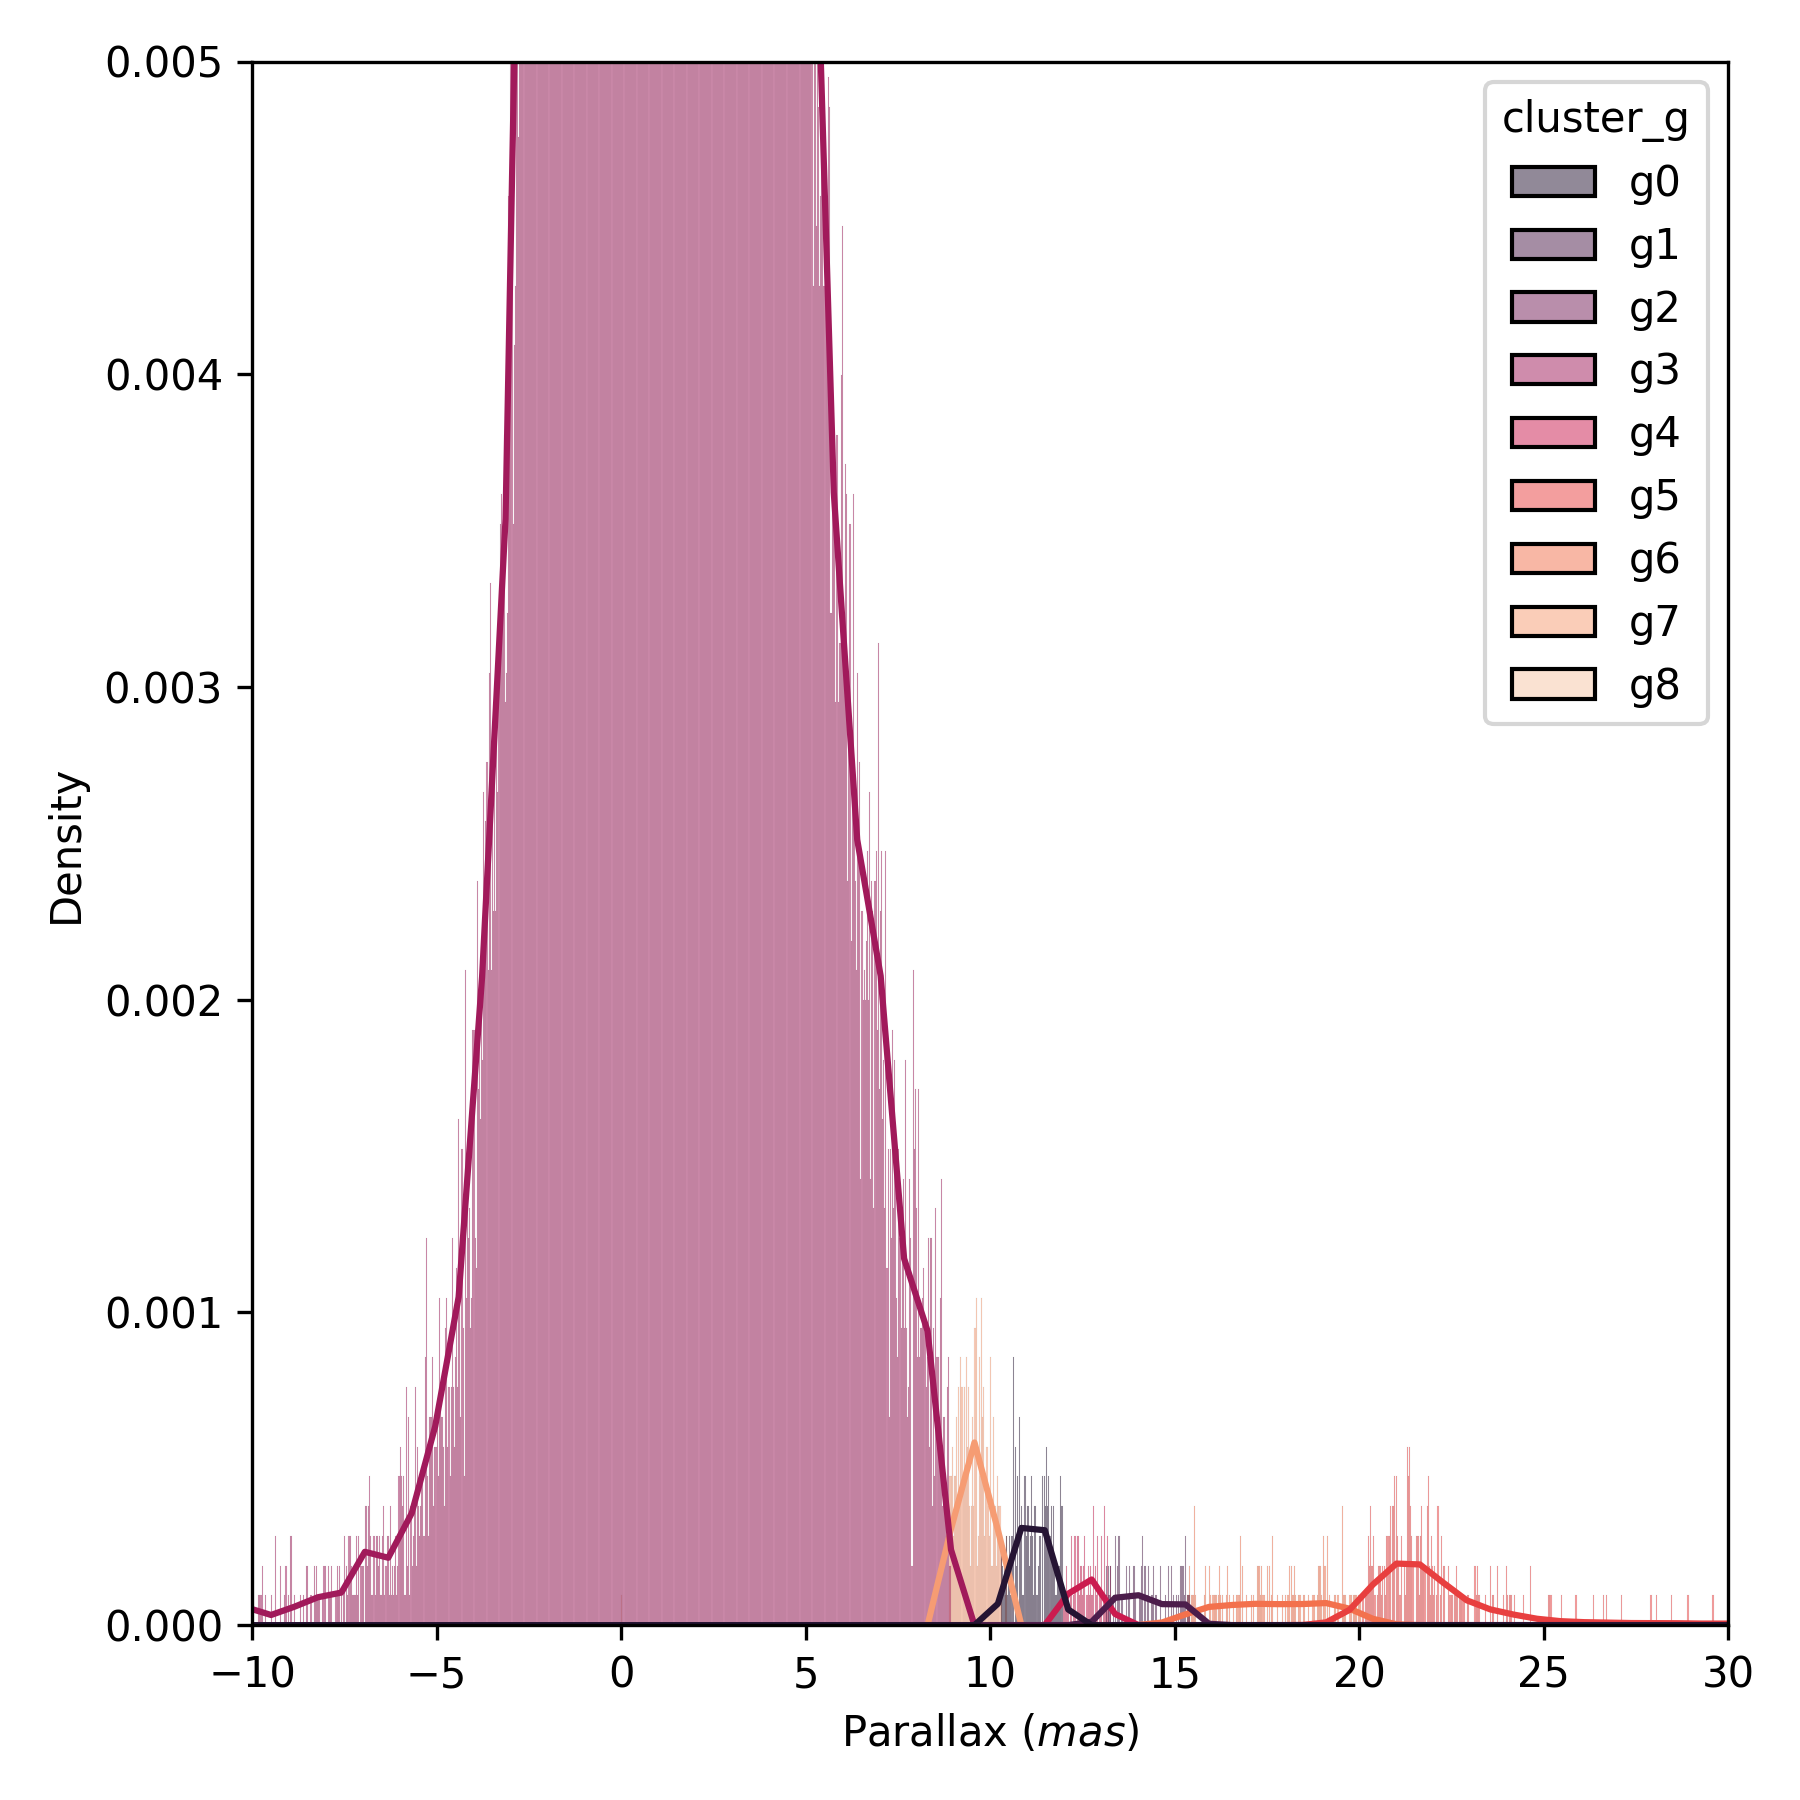
\includegraphics[width=\textwidth]{../figures/melotte_25/dec_parallax_melotte_25.png}
    \end{subfigure}
    \hfill
    \begin{subfigure}[t]{0.30\textwidth}
      \centering
      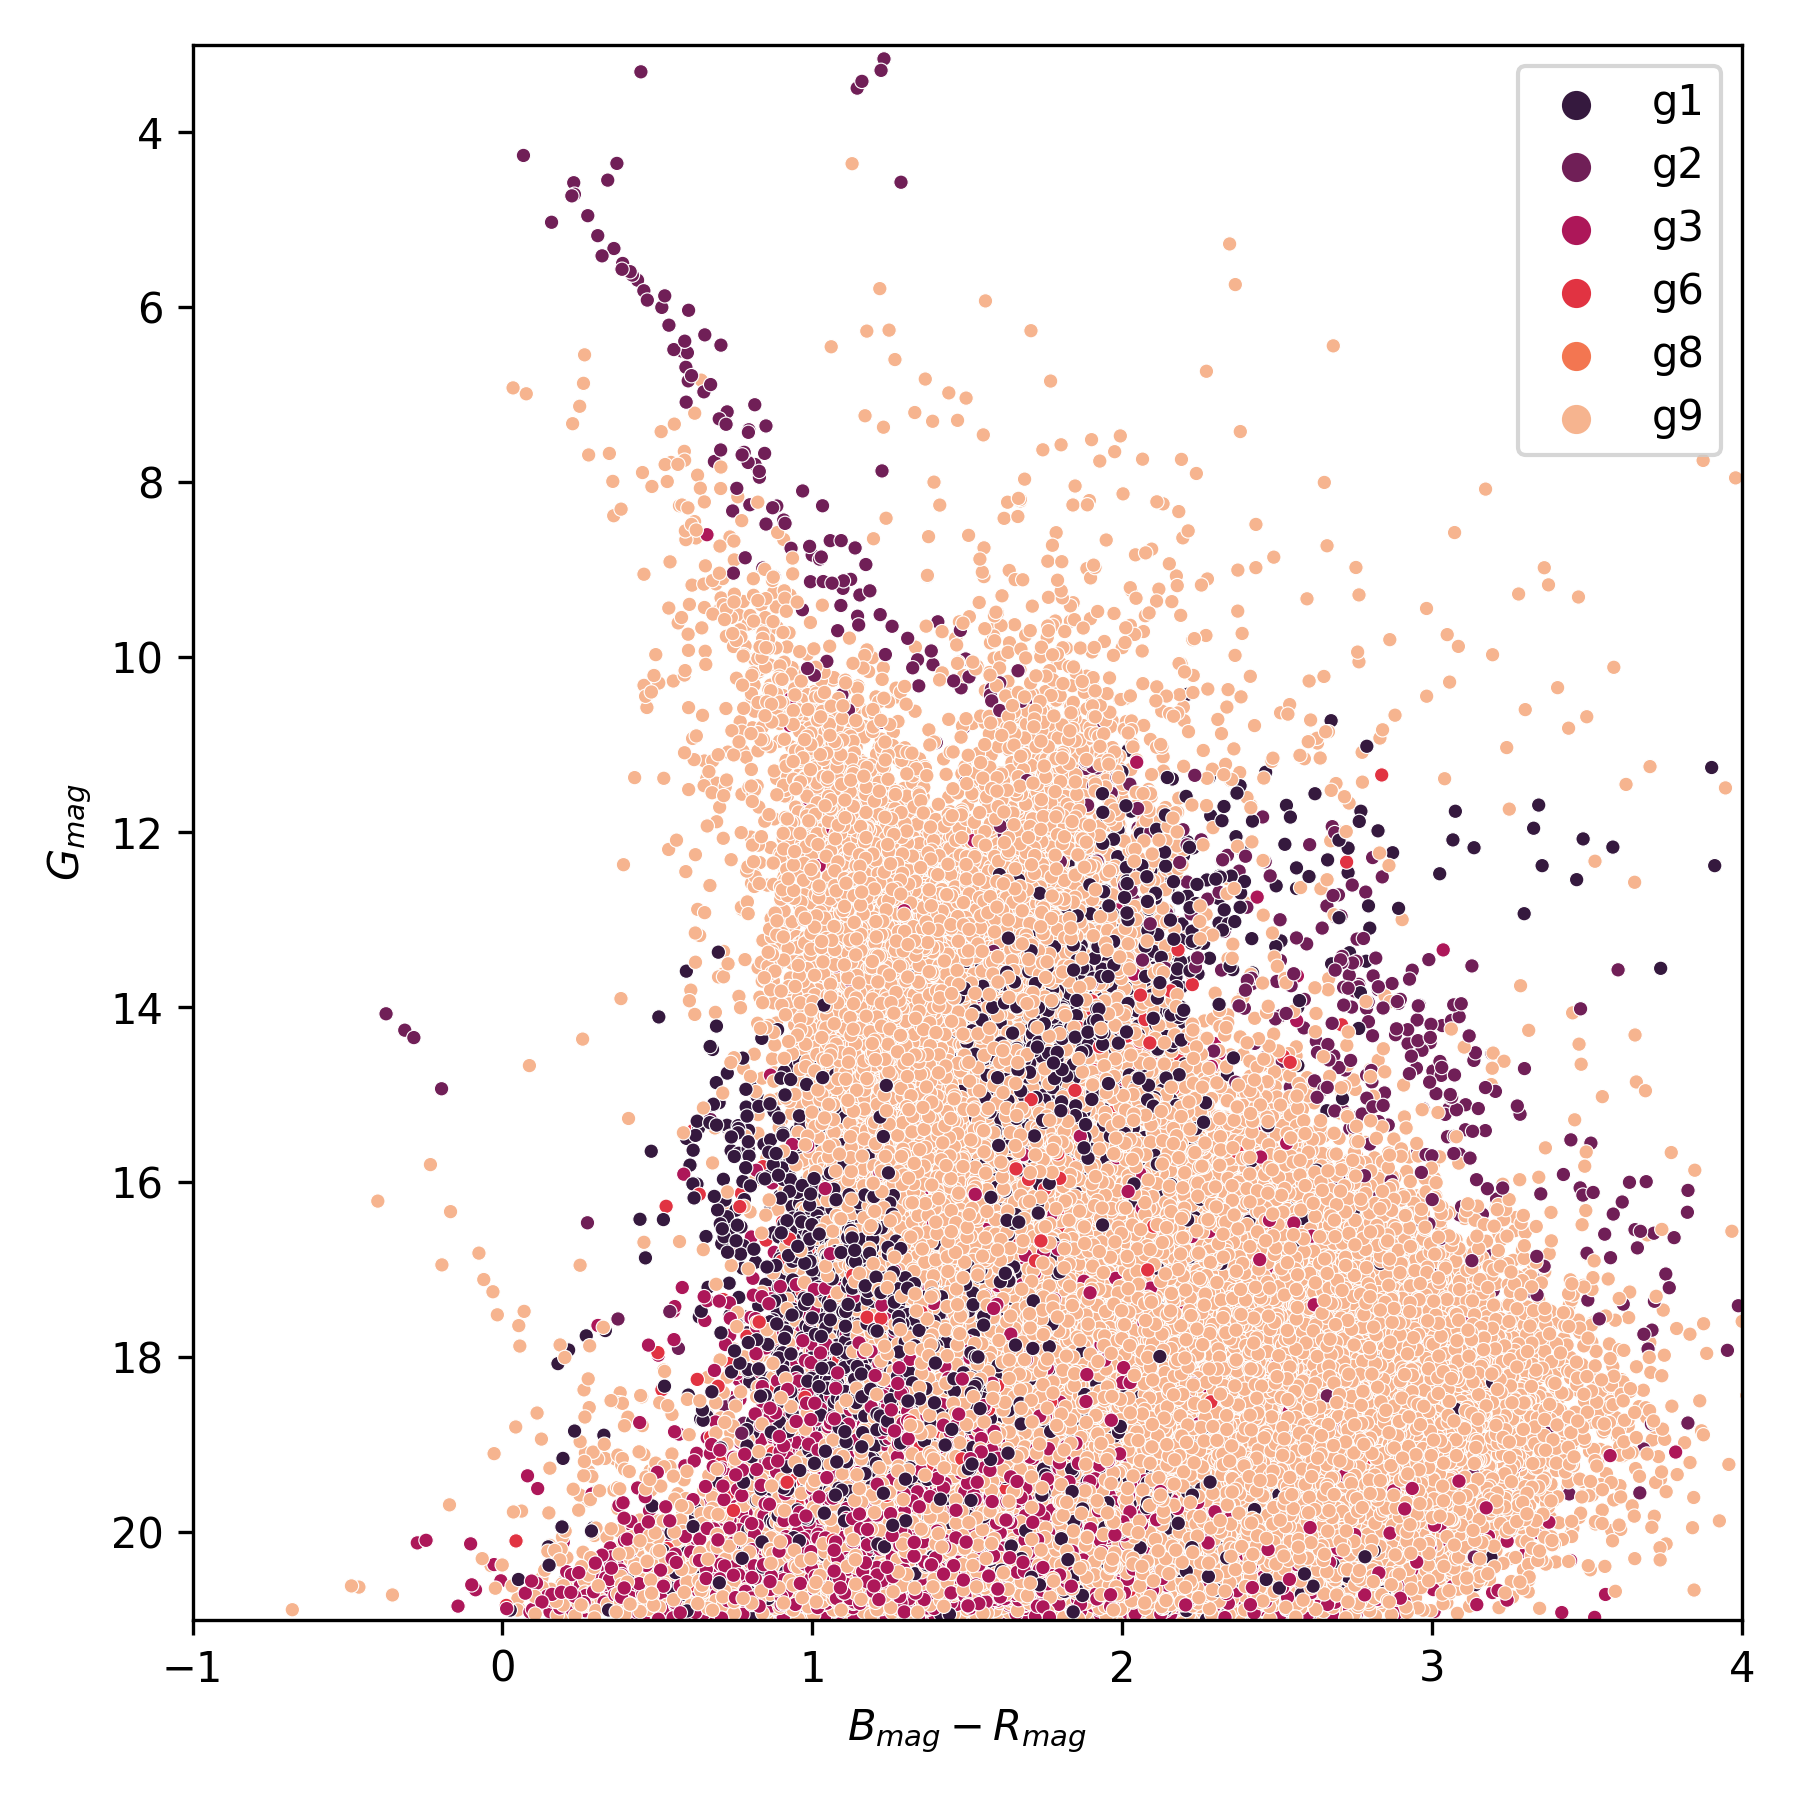
\includegraphics[width=\textwidth]{../figures/melotte_25/dec_hr_diagram_melotte_25.png}
    \end{subfigure}
  \end{subfigure}
  \caption{Melotte 25 characterization using the DEC model.
           From the left to the right: proper motion configuration
           space, parallax histogram and H-R diagram.}
  \label{fig:result_melotte_25_dec}
\end{figure}

Table \ref{tab:hyperparameters_melotte_25} shows the hyperparameters
used for the characterization.

\begin{table}[h]
  \begin{center}
    \begin{tabular}{l|c}
      \textbf{Hyperparameter} & \textbf{Value} \\
      \hline
      Number of Clusters & 9 \\
      Clustering Layer & $\left[ 50, 50, 40 \right]$ \\
      Kernel Initializer Seed & 11 \\
      Quantil Threshold & 0.1 \\
    \end{tabular}
    \caption{Melotte 25 DEC hyperparameters.}
    \label{tab:hyperparameters_melotte_25}
  \end{center}
\end{table}

\section{RESULTS DISCUSSION}

We have applied our proposed method to clusters with different typologies:

\begin{itemize}
  \item NGC 2516 (Ap. \ref{sec:ngc2516}) has it proper motion center deviated from the origin but
        it is embedded inside a big cloud of stars with similar proper motions.
  \item NGC 2632 (Ap. \ref{sec:ngc2632}), in addition to Melotte 22, ia s cluster whose proper motion center
        is not located at the origin and has a well separated parallax center.
  \item NGC 2682 (Ap. \ref{sec:ngc2682}), on the other hand, has its parallax centered within the region's gaussian,
        which complicates its detection although its proper motion center is deviated from the origin.
  \item Melotte 22 (Ap. \ref{sec:melotte22}), as well as Melotte 25, is a cluster closer to us than the other.
        That makes its membership stars to be more scattered than previous clusters which are more compact.
\end{itemize}

All these clusters have a wide variety of diameters, from 25 to 330 arcmin,
as well as the number of stars that belong to them. NGC 2682 has 3,000 stars
while Melotte 25 is located inside a region with more than 400,000 stars.
More information about the studied clusters is available in Table \ref{tab:clusters_summary}.

\begin{table}[htbp]
  \begin{center}
    \resizebox{\columnwidth}{!}{
      \begin{tabular}{l|c|c|c|c}
        \textbf{OC} & \emph{$\alpha$ J2000 $(degrees)$} & \emph{$\delta$ J2000 $(degrees)$} & \emph{Radius $(arcmin)$} & \emph{\# stars} \\
        \hline
        NGC 2516 & 119.517 & -60.753 & 15 & 12,869 \\
        NGC 2632 & 130.1 & 19.667 & 35 & 13,167 \\
        NGC 2682 & 132.825 & 11.8 & 12.5 & 2,839 \\
        Melotte 22 & 56.75 & 24.117 & 60 & 61,552 \\
        Melotte 25 & 66.725 & 15.867 & 165 & 433,996 \\
      \end{tabular}
    }
    \caption{Righ ascension, declination, radius and number of stars of studied clusters.
             The number of stars corresponds to those stars contained within a cone of center
             $(\alpha, \delta)$ and raius the cluster's radius multiplied by a factor of 1.5.}
    \label{tab:clusters_summary}
  \end{center}
\end{table}

In all cases, the model has resolved properly the identity of the cluster
and has characterized the membership stars, giving compatible results
with the ones obtained with classic procedures and VO tools.

Compared with the mentioned tools, our model can be categorized as a
non-parameterized model since it does not depend on parameters referred
to the cluster itself but only hyperparameters such as the initial number
of clusters to be found, or the structure of the Clustering Layer used by DEC model.

The proposed method is also non-supervised since we do not need to tell the model
which stars belong to the cluster or assist it while its training stage.

Only at the end of the characterization, a fine tuning driven by the user,
can be applied in order to improve the selection by discarding those
stars which fall outside the given quantiles.

In any case, we do not make assumptions about the cluster profile,
something that we have to take into account when using VO tools.
This is another evidence that our model is non-parameterized.

\section{CONCLUSIONS}

From the results shown in Section \ref{sec:results}, we can say that, in general,
our model works fine identifying and characterizing open clusters.
So we have succeeded building a model non-parameterized and non-supervised
for open cluster characterization. However, some improvements should be done
in order to improve its accuracy and precision.

We have built a non-parameterized model since the user is not required to provide
any information about the cluster profile or its properties.
Nevertheless some tweaks can be done regarding the cluster, like changing the initial
number of clusters or modifying the clustering layer structure in order to improve
the final characterization.

Another key point in our model is the initializer kernel.
This kernel prepares data before passing it to the ANN
and the results may vary significantly depending on this kernel.
This is something to avoid, so an improvement to solve this issue is necessary
in order to have a reliable model which does not depend on the dataset order.

Despite that, comparing our method with Clusterix, we can still say that the
number of parameters (or hyperparameters) in our model is smaller and that
we do not need previous knowledge about the studied cluster.
That makes easier to test different configurations and automate the process.

\subsection{FURTHER RESEARCH}

One open point to do from now is testing the model with a wider range of clusters.
In general we could think of applying it to the whole VizieR catalogue.
That way we could have a better idea about the current limitations of our model
and we could make some adjustments to improve it. We could determine with higher
accuracy the typologies that our model works well with, and which ones the model
does not resolve properly. Furthermore, we could stablish different sets of
hyperparameters regarding the typology of the cluster.

With our model, new uncatalogued clusters arise from the data apart of the main ones.
Hence, it is also interesting the individual study of these new clusters.

Another possible change in our model would be using DBSCAN instead of K-Means
as our initial clustering algorithm. Maybe this algorithm gives us a better starting
point for the DEC model which could improve the results.

Finally, we have used the Gaia DR2 database as our data source for this work,
but recently the DR3 dataset has been released.
Therefore, it is evident the interest on testing our model with this new data.

\appendix
\section{APPENDIX}
\label{sec:appendix}

\subsection{NGC 2516}
\label{sec:ngc2516}

\begin{table}[htbp]
  \begin{center}
    \resizebox{\columnwidth}{!}{
      \begin{tabular}{l|c|c|c|c}
        \textbf{Method} & \emph{$\mu_{\alpha}$ $(mas/yr^{-1})$} & \emph{$\mu_{\delta}$ $(mas/yr^{-1})$} & \emph{$\varpi$ $(mas)$} & \emph{\# stars} \\
        \hline
        \textbf{Simbad} & -4.6579 $\pm$ 0.0075 & 11.1517 $\pm$ 0.0075 & 2.4118 $\pm$ 0.0006 & 1727 \\
        Clusterix & -4.652 $\pm$ 0.523 & 11.203 $\pm$ 0.454 & 2.409 $\pm$ 0.127 & 638 \\
        K-Means & -4.344 $\pm$ 0.14 & 9.507 $\pm$ 0.19 & 2.268 $\pm$ 0.01 & 1542 \\
        DEC & -4.426 $\pm$ 0.17 & 9.952 $\pm$ 0.20 & 2.436 $\pm$ 0.01 & 1532 \\
        \textbf{DEC (filt.)} & -4.502 $\pm$ 0.14 & 10.114 $\pm$ 0.17 & 2.392 $\pm$ 0.004 & 1072 \\
      \end{tabular}
    }
    \caption{NGC 2516 results.}
    \label{tab:app_results_ngc_2516}
  \end{center}
\end{table}

Table \ref{tab:app_results_ngc_2516} shows a results summary for NGC 2516.
The top row of Figure \ref{fig:app_result_ngc_2516_clusterix_kmeans} shows
the characterization using Clusterix+TOPCAT tools while the bottom row
shows eight clusters found by K-Means.

\begin{figure}[htbp]
  \centering
  \begin{subfigure}{\columnwidth}
    \centering
    \begin{subfigure}[t]{0.30\textwidth}
      \centering
      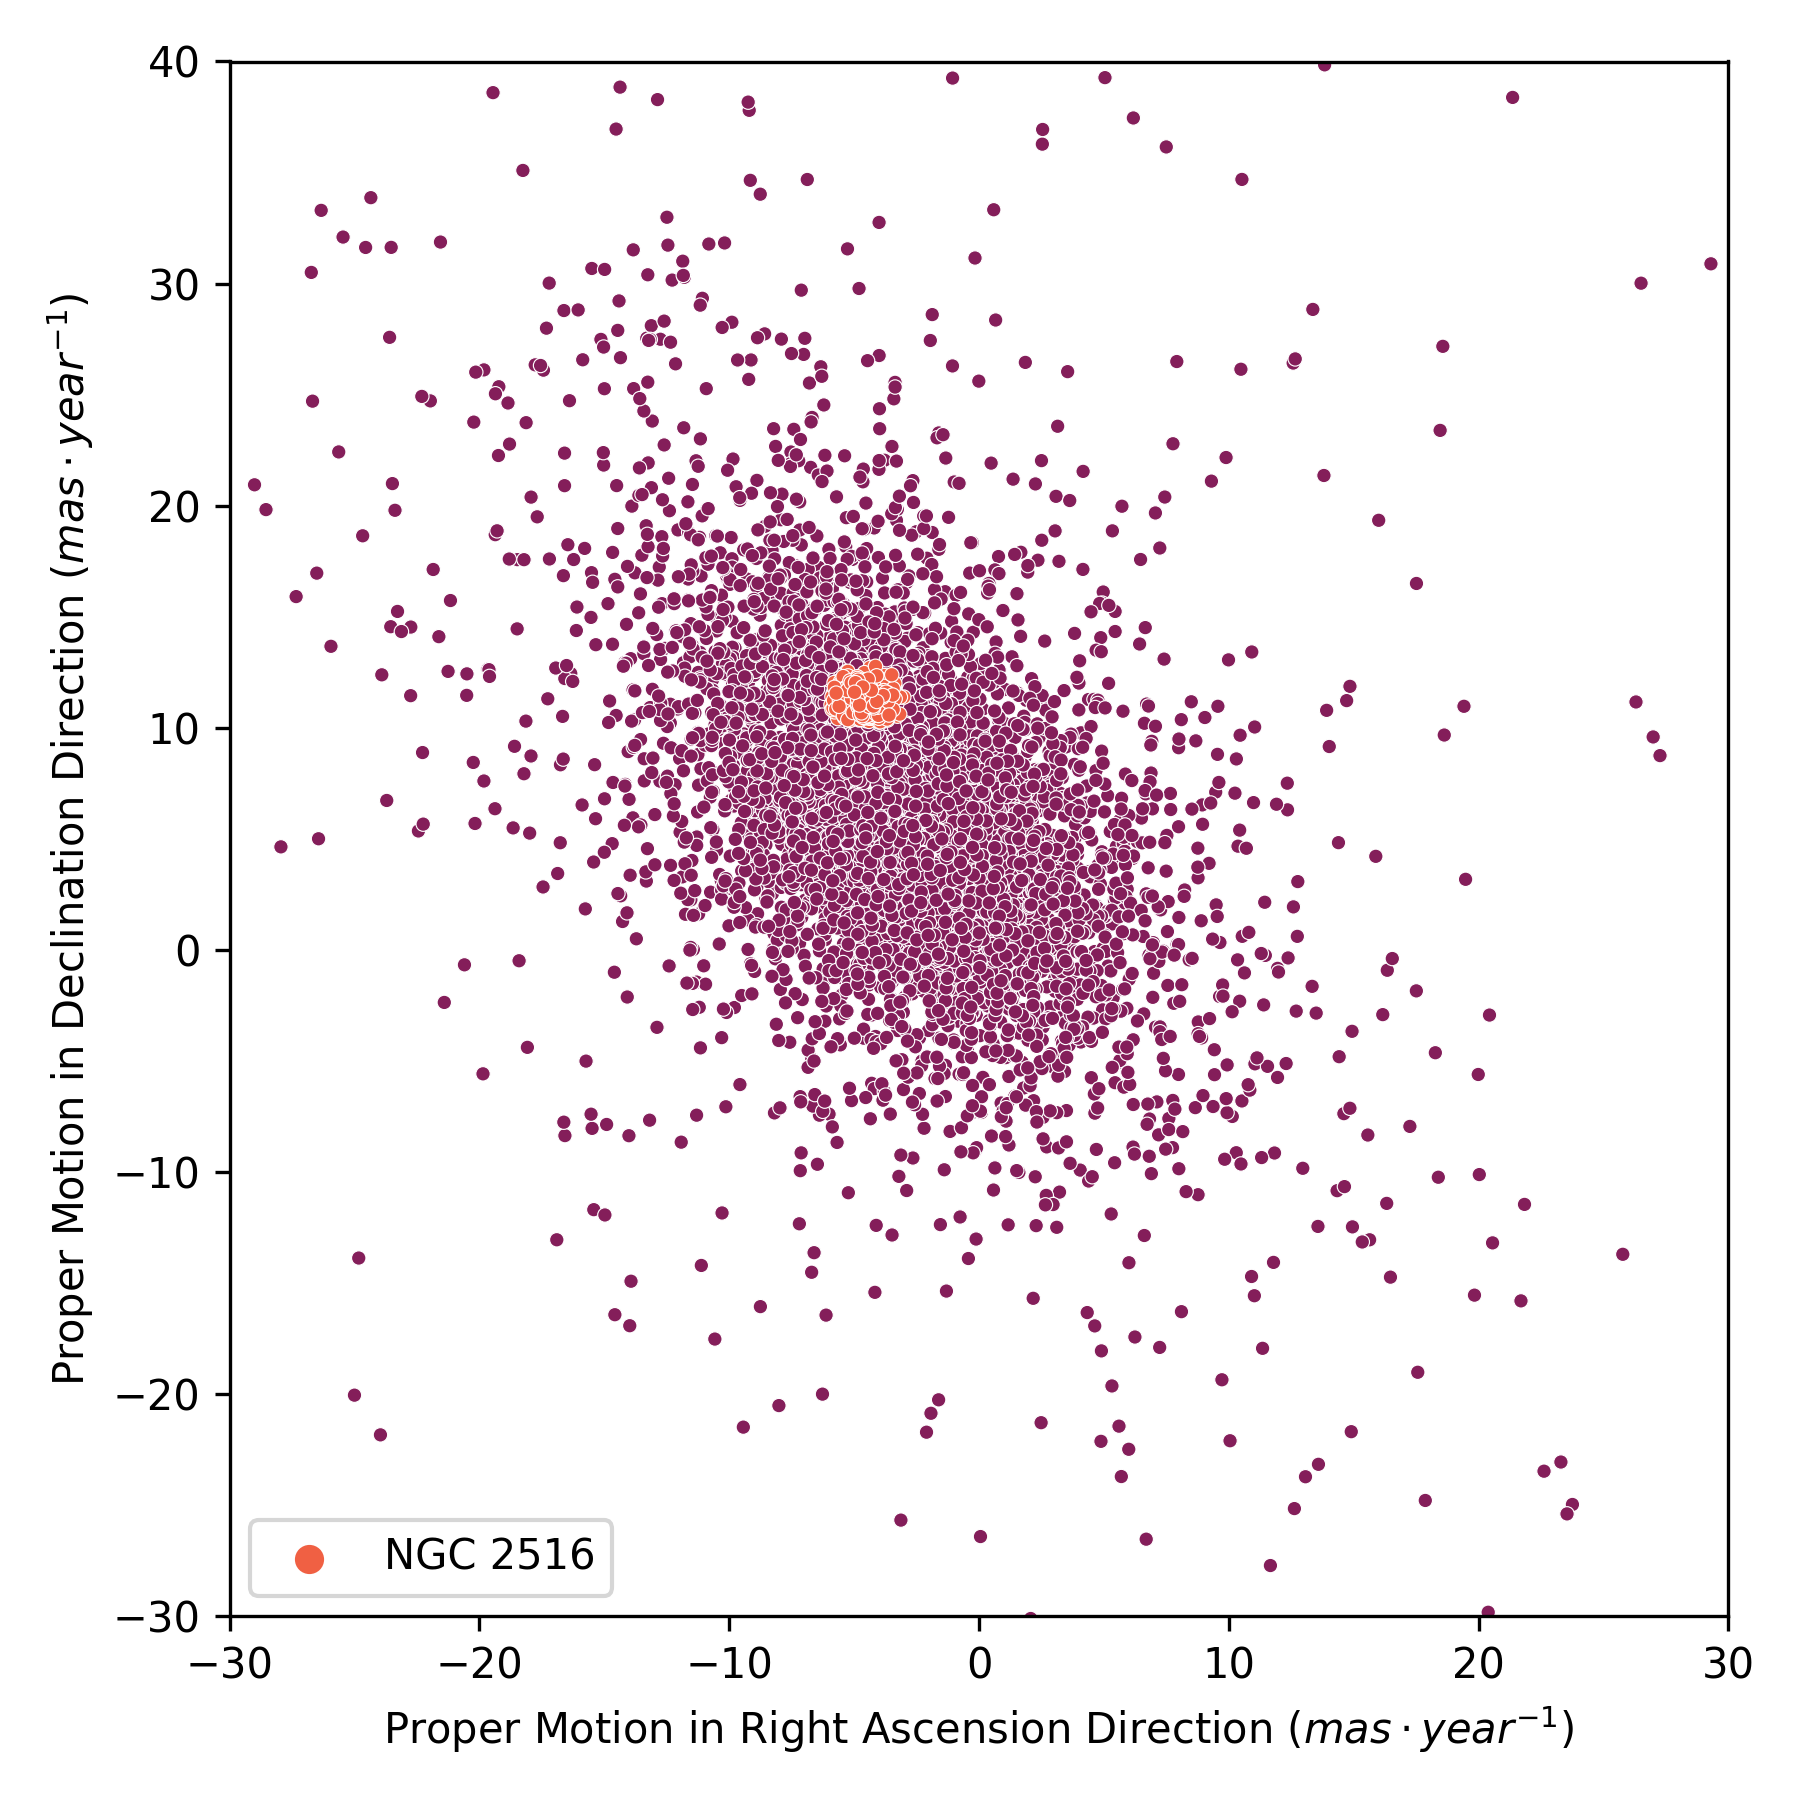
\includegraphics[width=\textwidth]{../figures/ngc_2516/pm_ngc_2516.png}
    \end{subfigure}
    \hfill
    \begin{subfigure}[t]{0.30\textwidth}
      \centering
      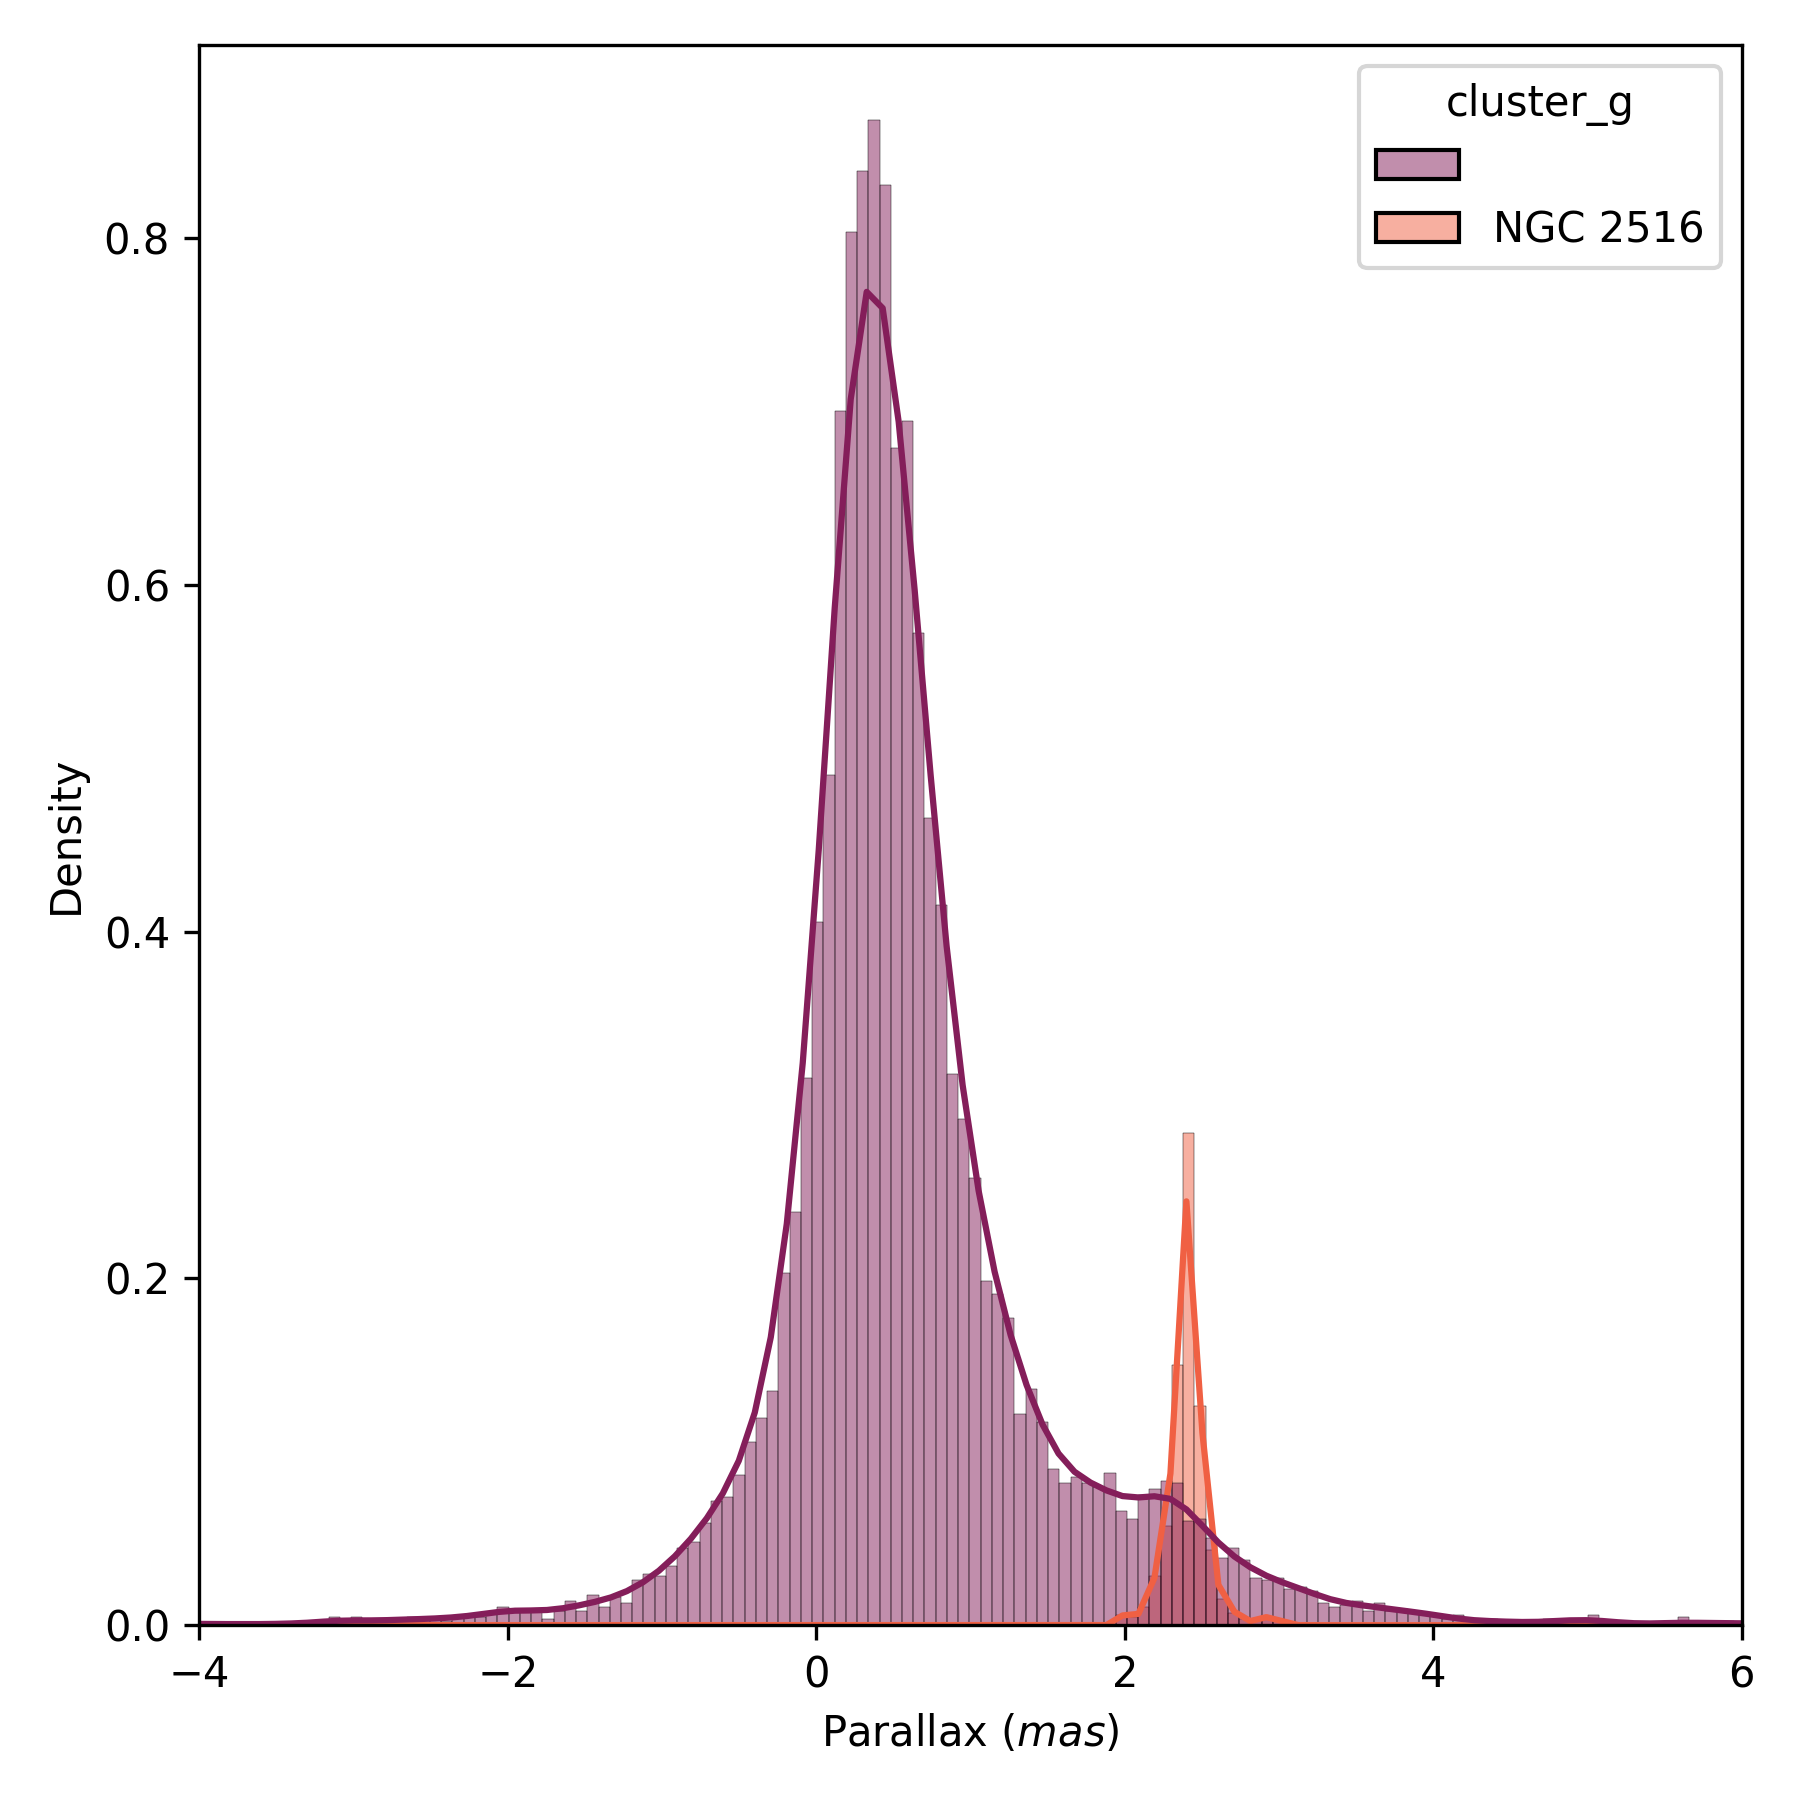
\includegraphics[width=\textwidth]{../figures/ngc_2516/parallax_ngc_2516.png}
    \end{subfigure}
    \hfill
    \begin{subfigure}[t]{0.30\textwidth}
      \centering
      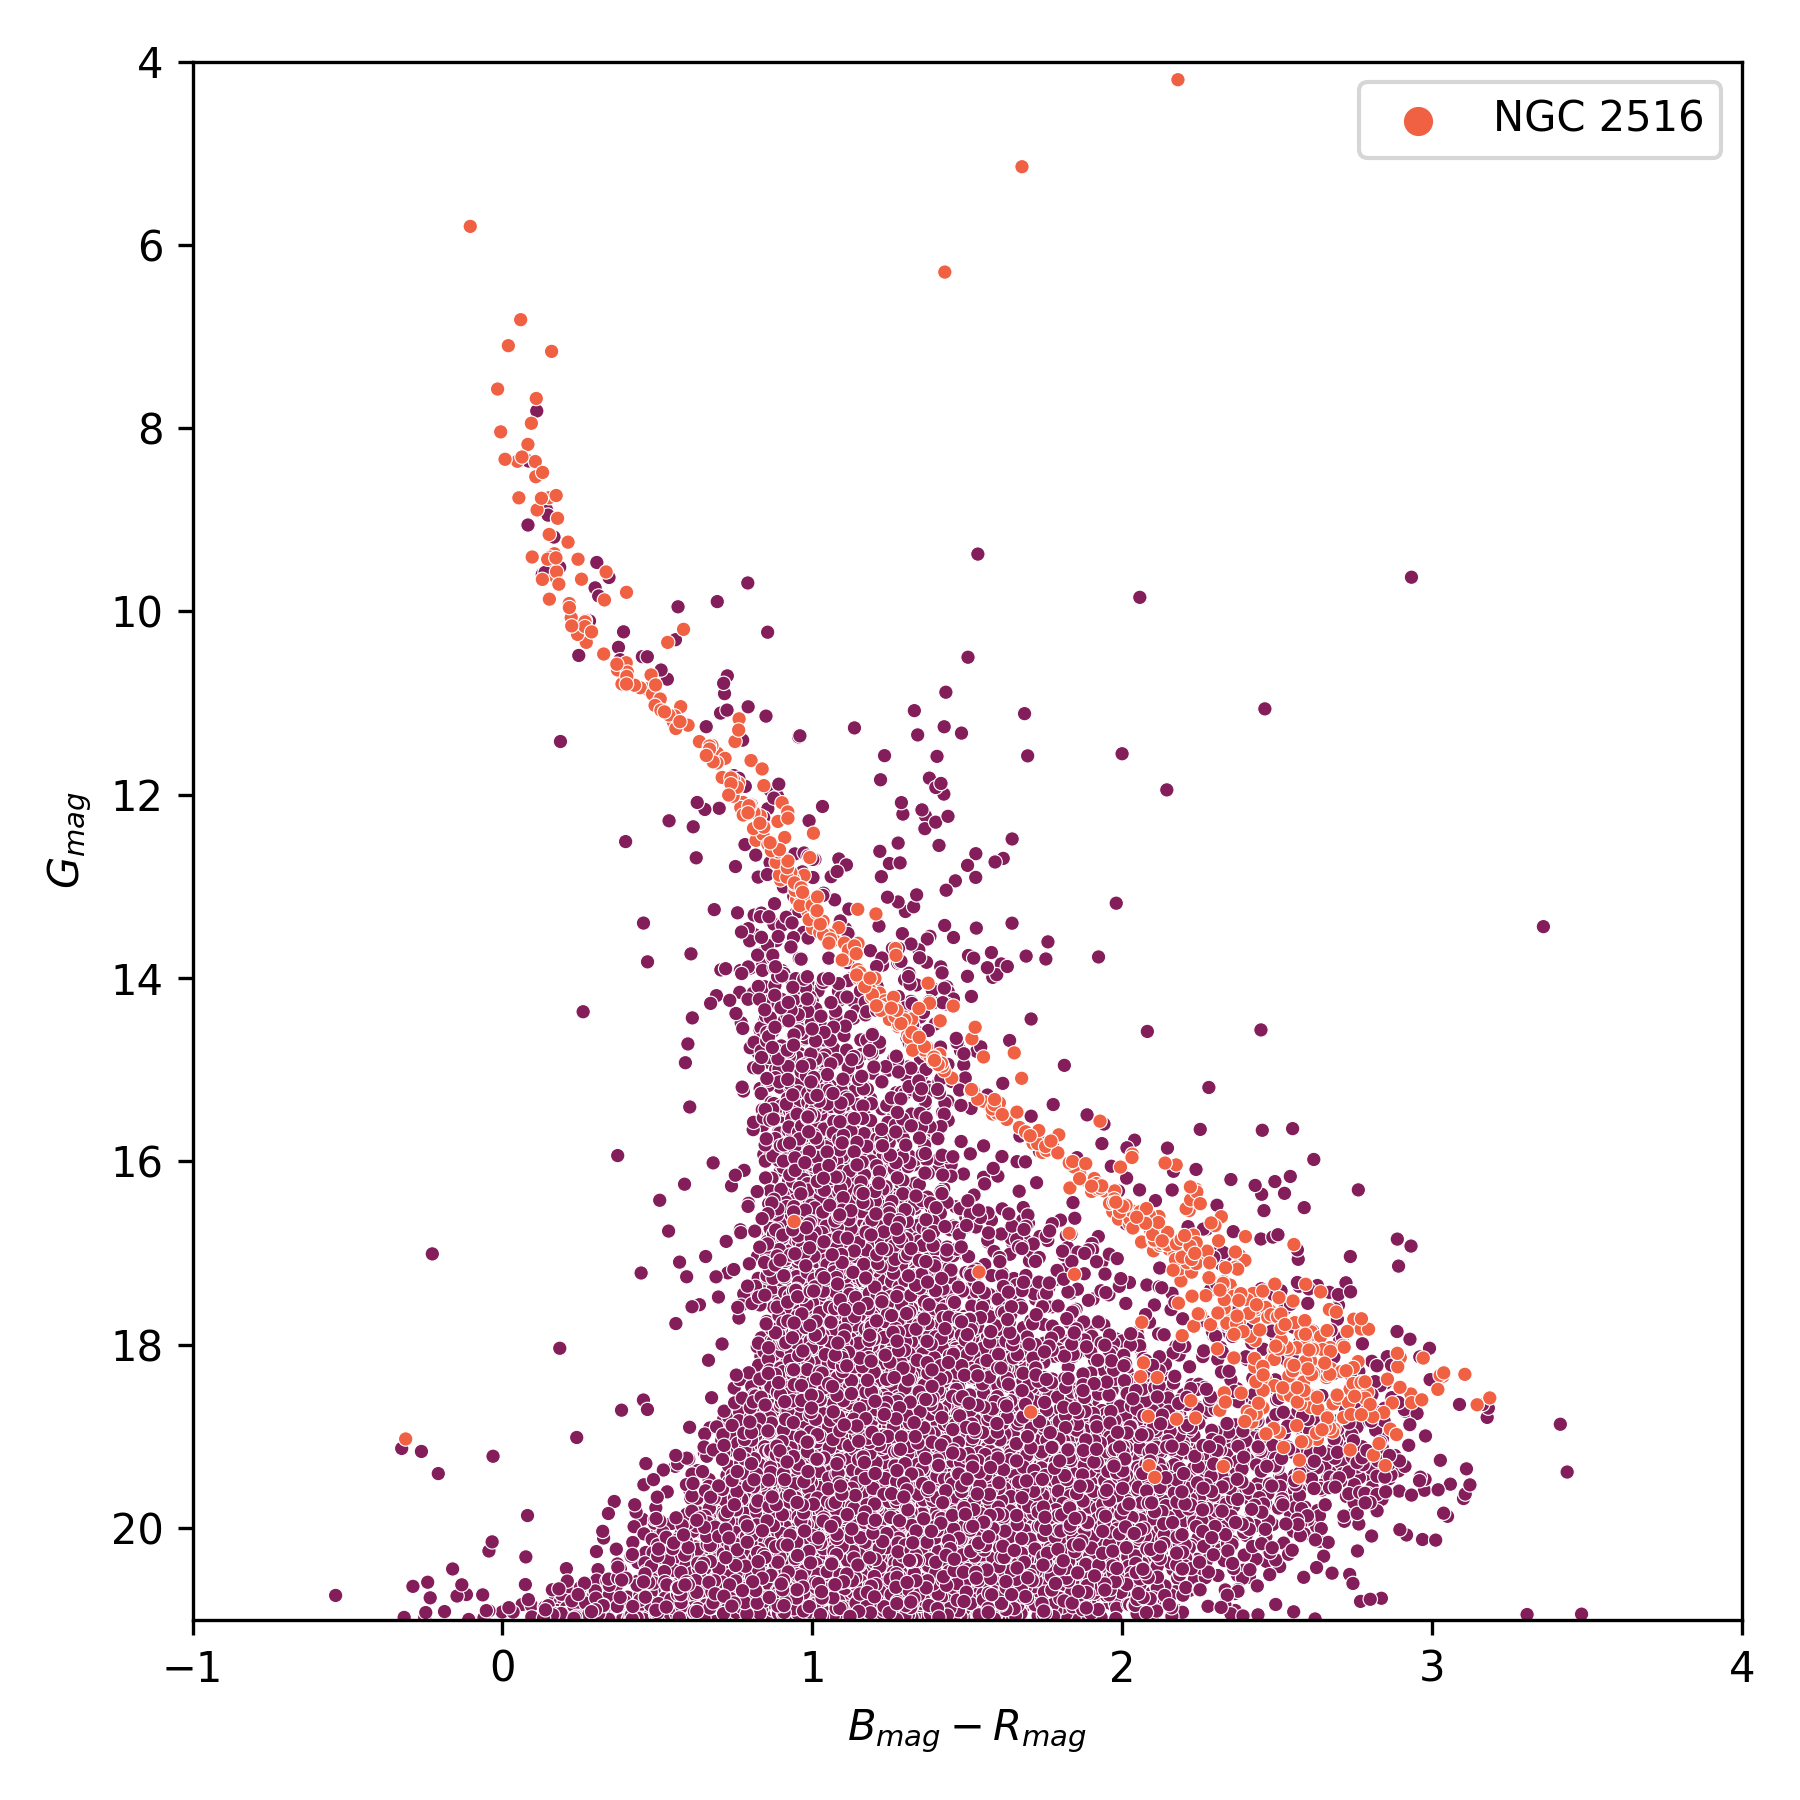
\includegraphics[width=\textwidth]{../figures/ngc_2516/hr_diagram_ngc_2516.png}
    \end{subfigure}
  \end{subfigure}
  \centering
  \begin{subfigure}{\columnwidth}
    \centering
    \begin{subfigure}[t]{0.30\textwidth}
      \centering
      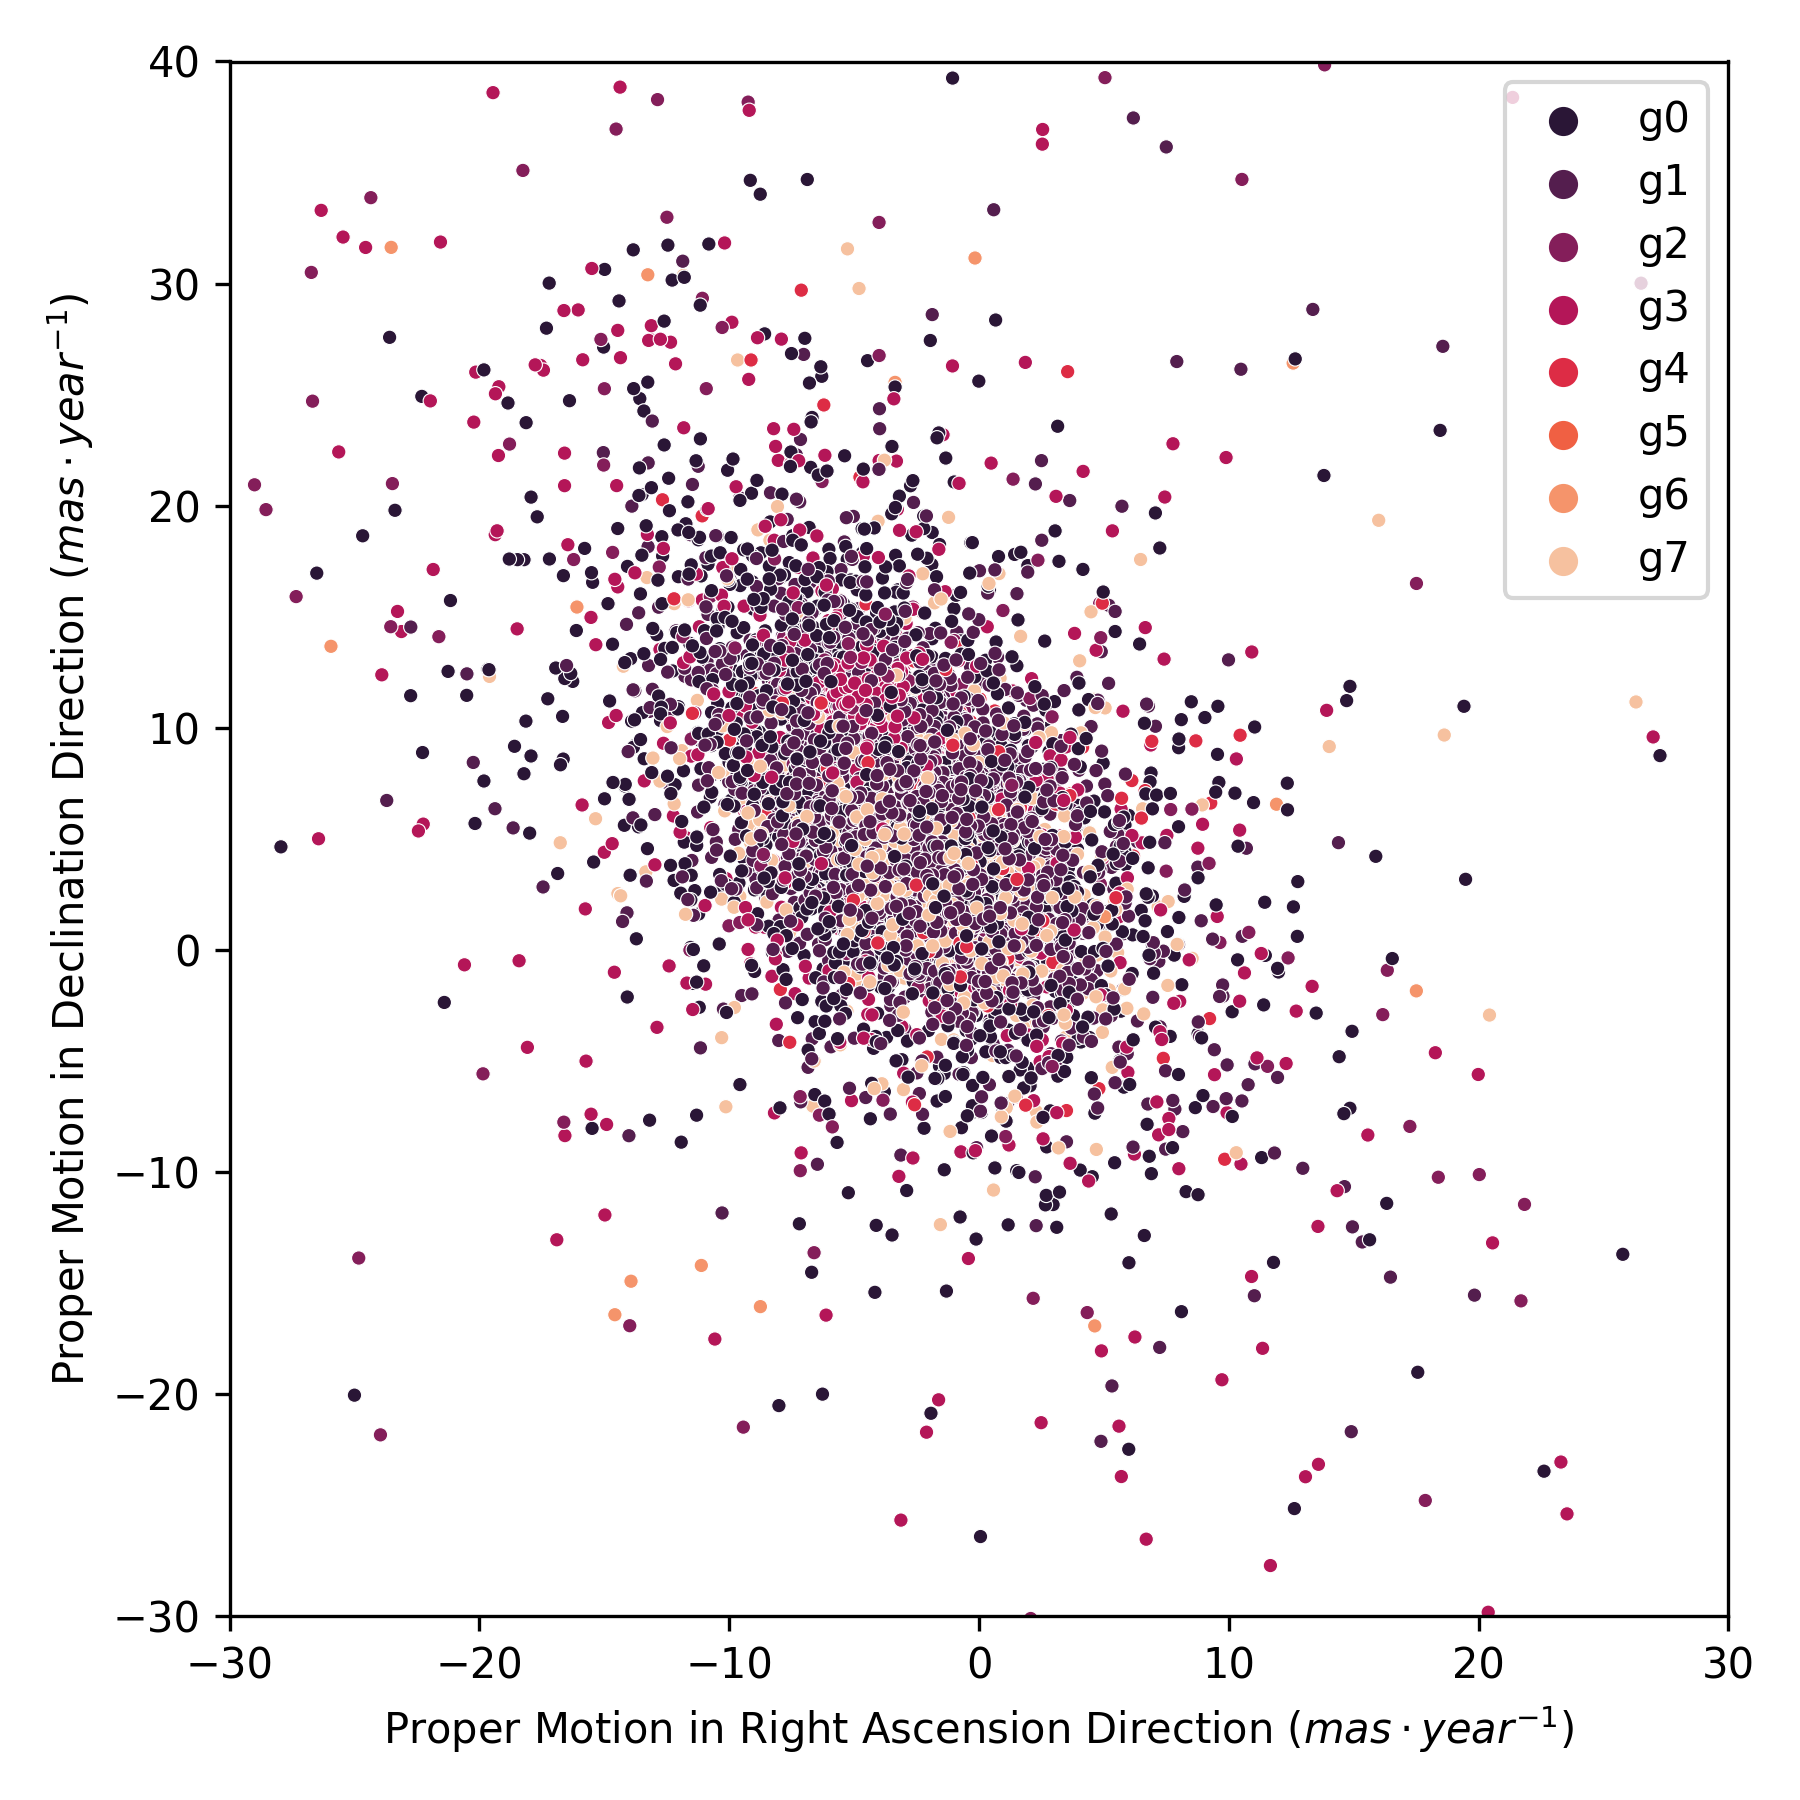
\includegraphics[width=\textwidth]{../figures/ngc_2516/kmeans_pm_ngc_2516.png}
    \end{subfigure}
    \hfill
    \begin{subfigure}[t]{0.30\textwidth}
      \centering
      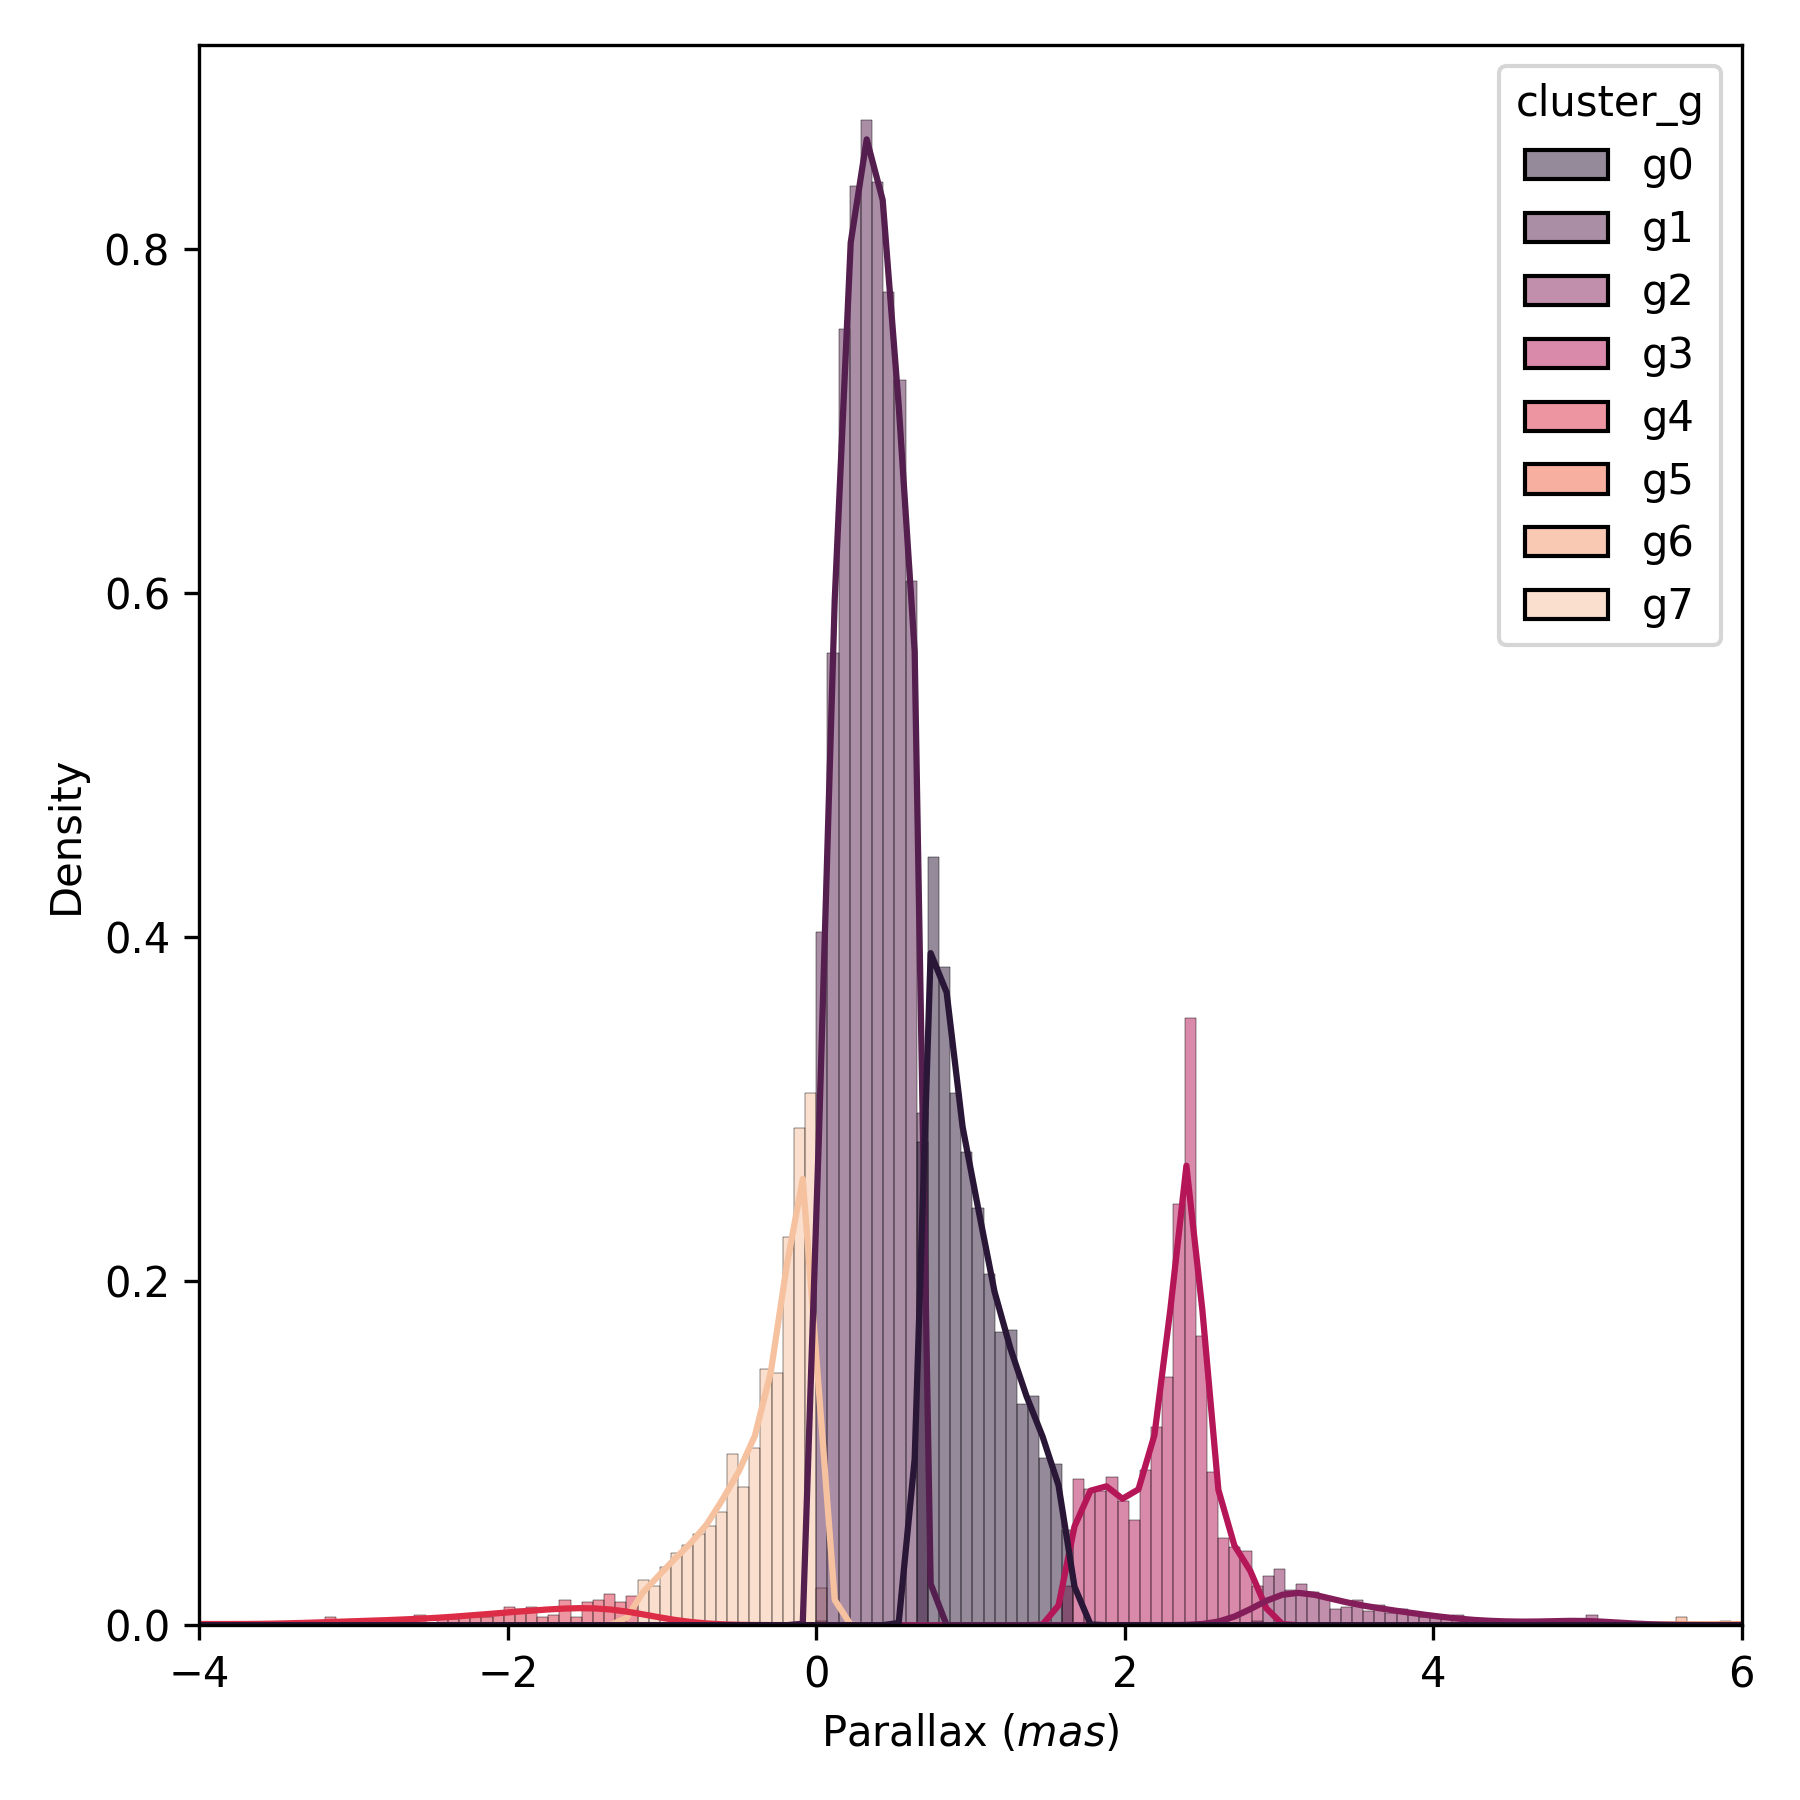
\includegraphics[width=\textwidth]{../figures/ngc_2516/kmeans_parallax_ngc_2516.png}
    \end{subfigure}
    \hfill
    \begin{subfigure}[t]{0.30\textwidth}
      \centering
      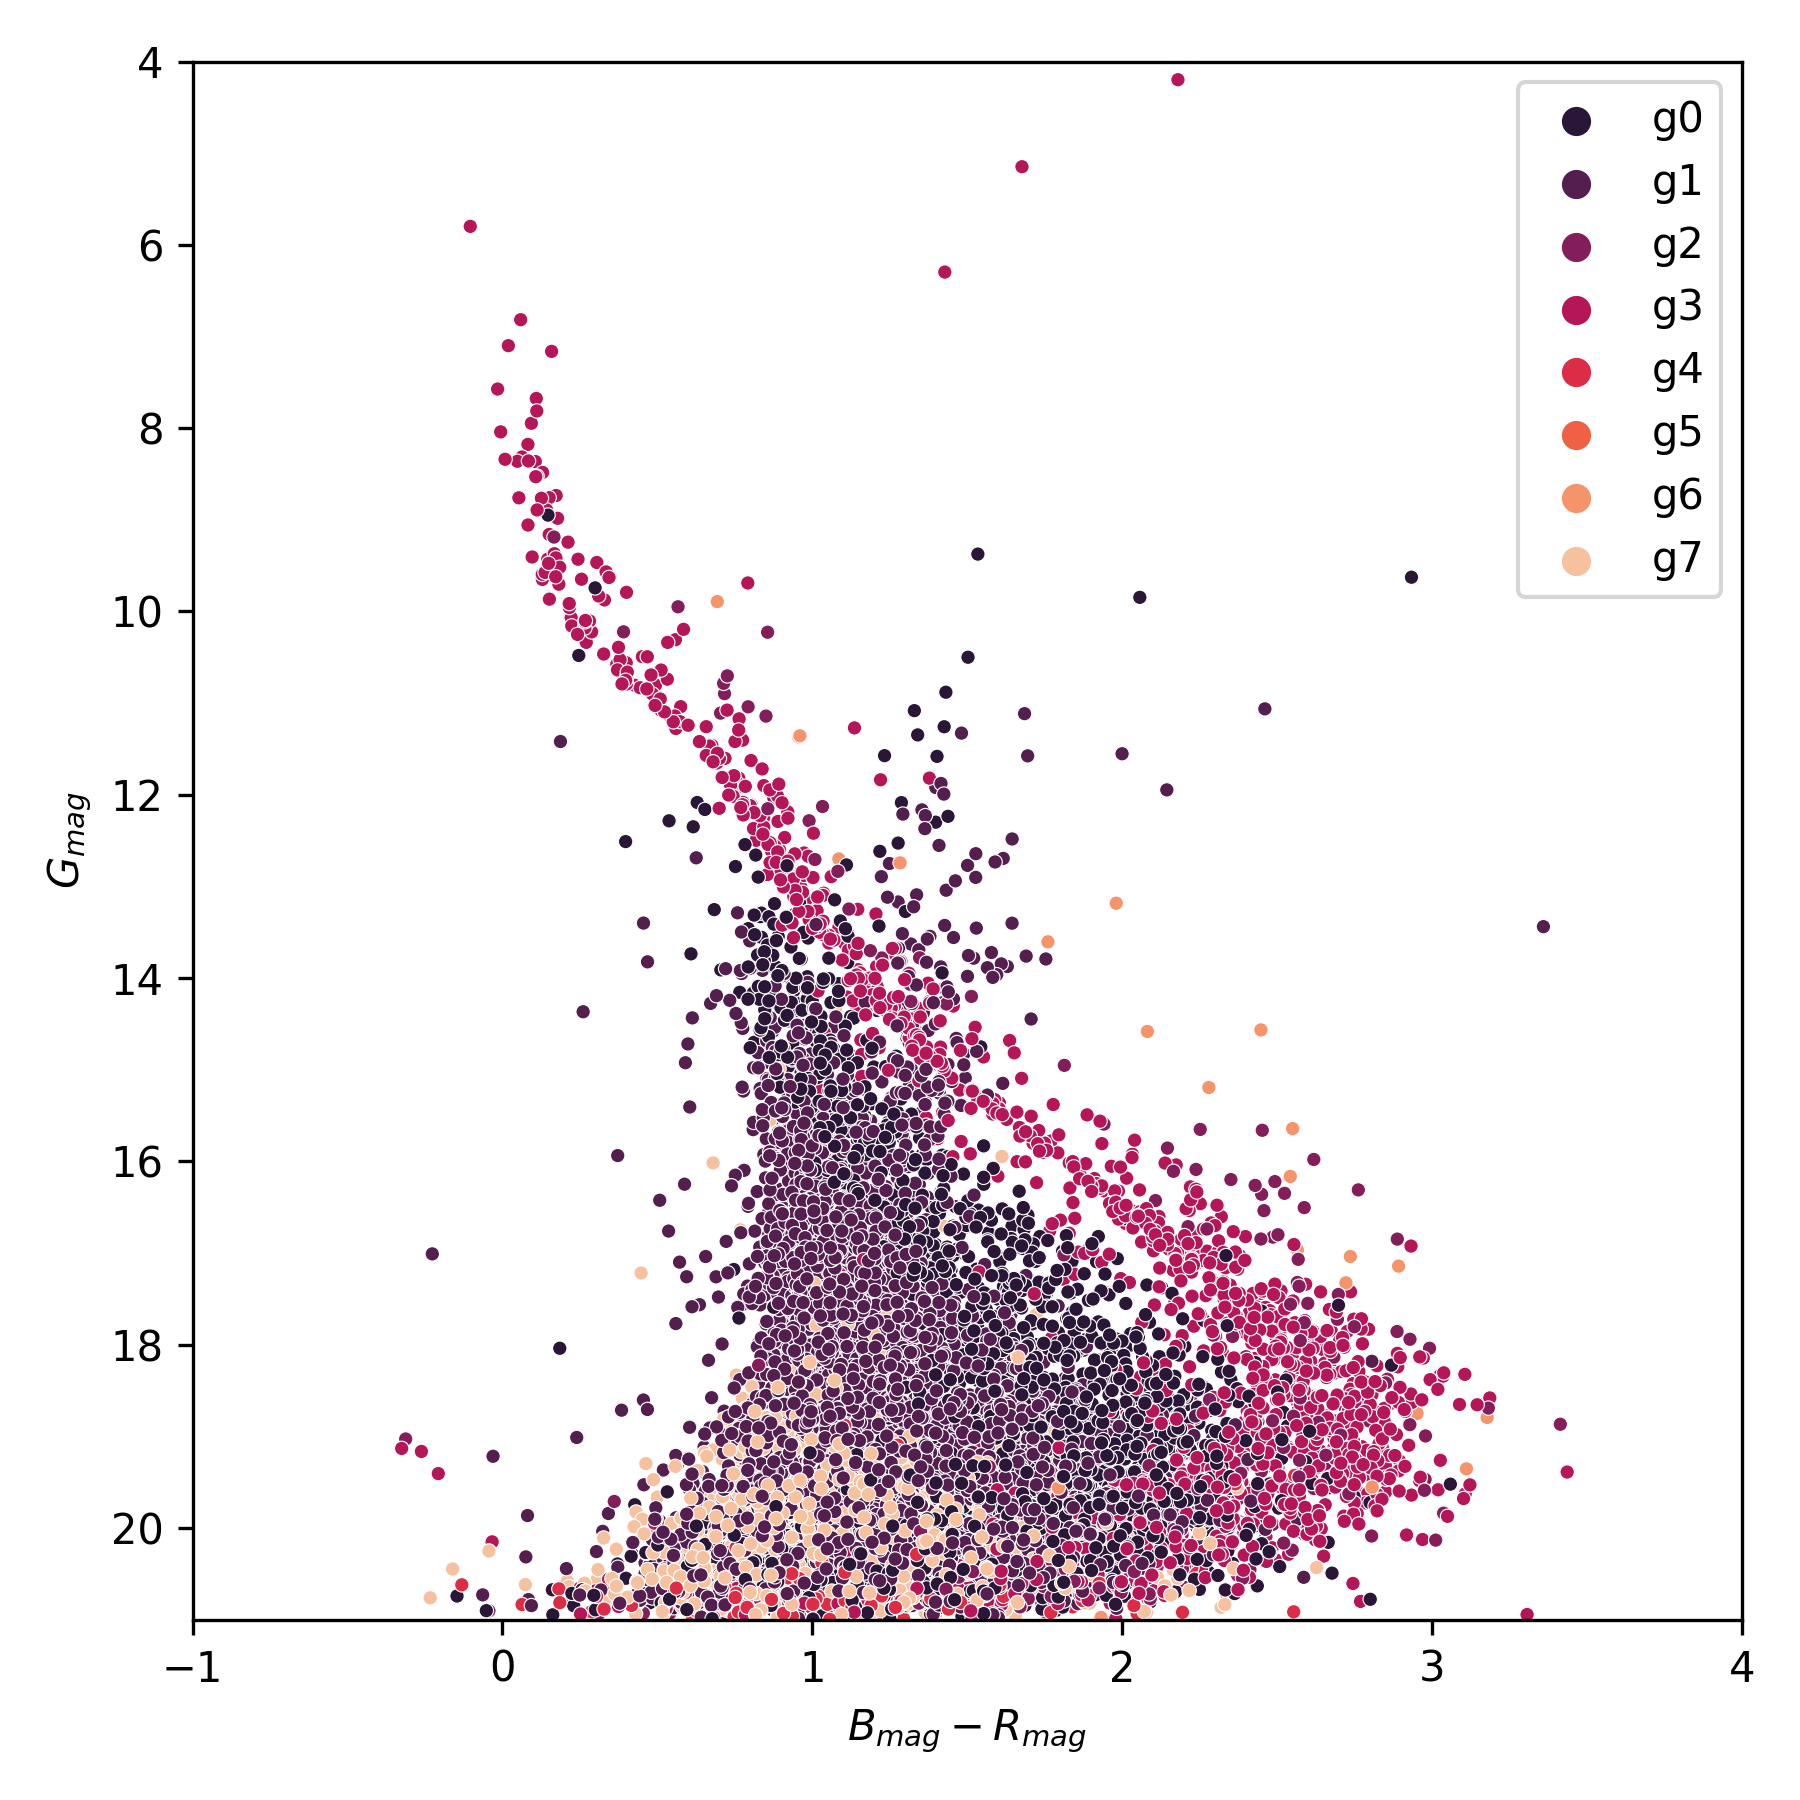
\includegraphics[width=\textwidth]{../figures/ngc_2516/kmeans_hr_diagram_ngc_2516.png}
    \end{subfigure}
  \end{subfigure}
  \caption{NGC 2516 characterization.
           Top: Clusterix+TOPCAT. Bottom: K-Means (\emph{g3}).}
  \label{fig:app_result_ngc_2516_clusterix_kmeans}
\end{figure}

Figure \ref{fig:app_result_ngc_2516_dec} shows the groups found using the
DEC model (top row) and the DEC model filtered (bottom row).
K-Means and DEC have labeled NGC 2516 as \emph{g3}. Although in general,
groups between K-Means and DEC models may not match.
Hyperparameters used in this characterization are listed in Table
\ref{tab:app_hyperparameters_ngc_2516}.

\begin{figure}[htbp]
  \centering
  \begin{subfigure}{\columnwidth}
    \centering
    \begin{subfigure}[t]{0.30\textwidth}
      \centering
      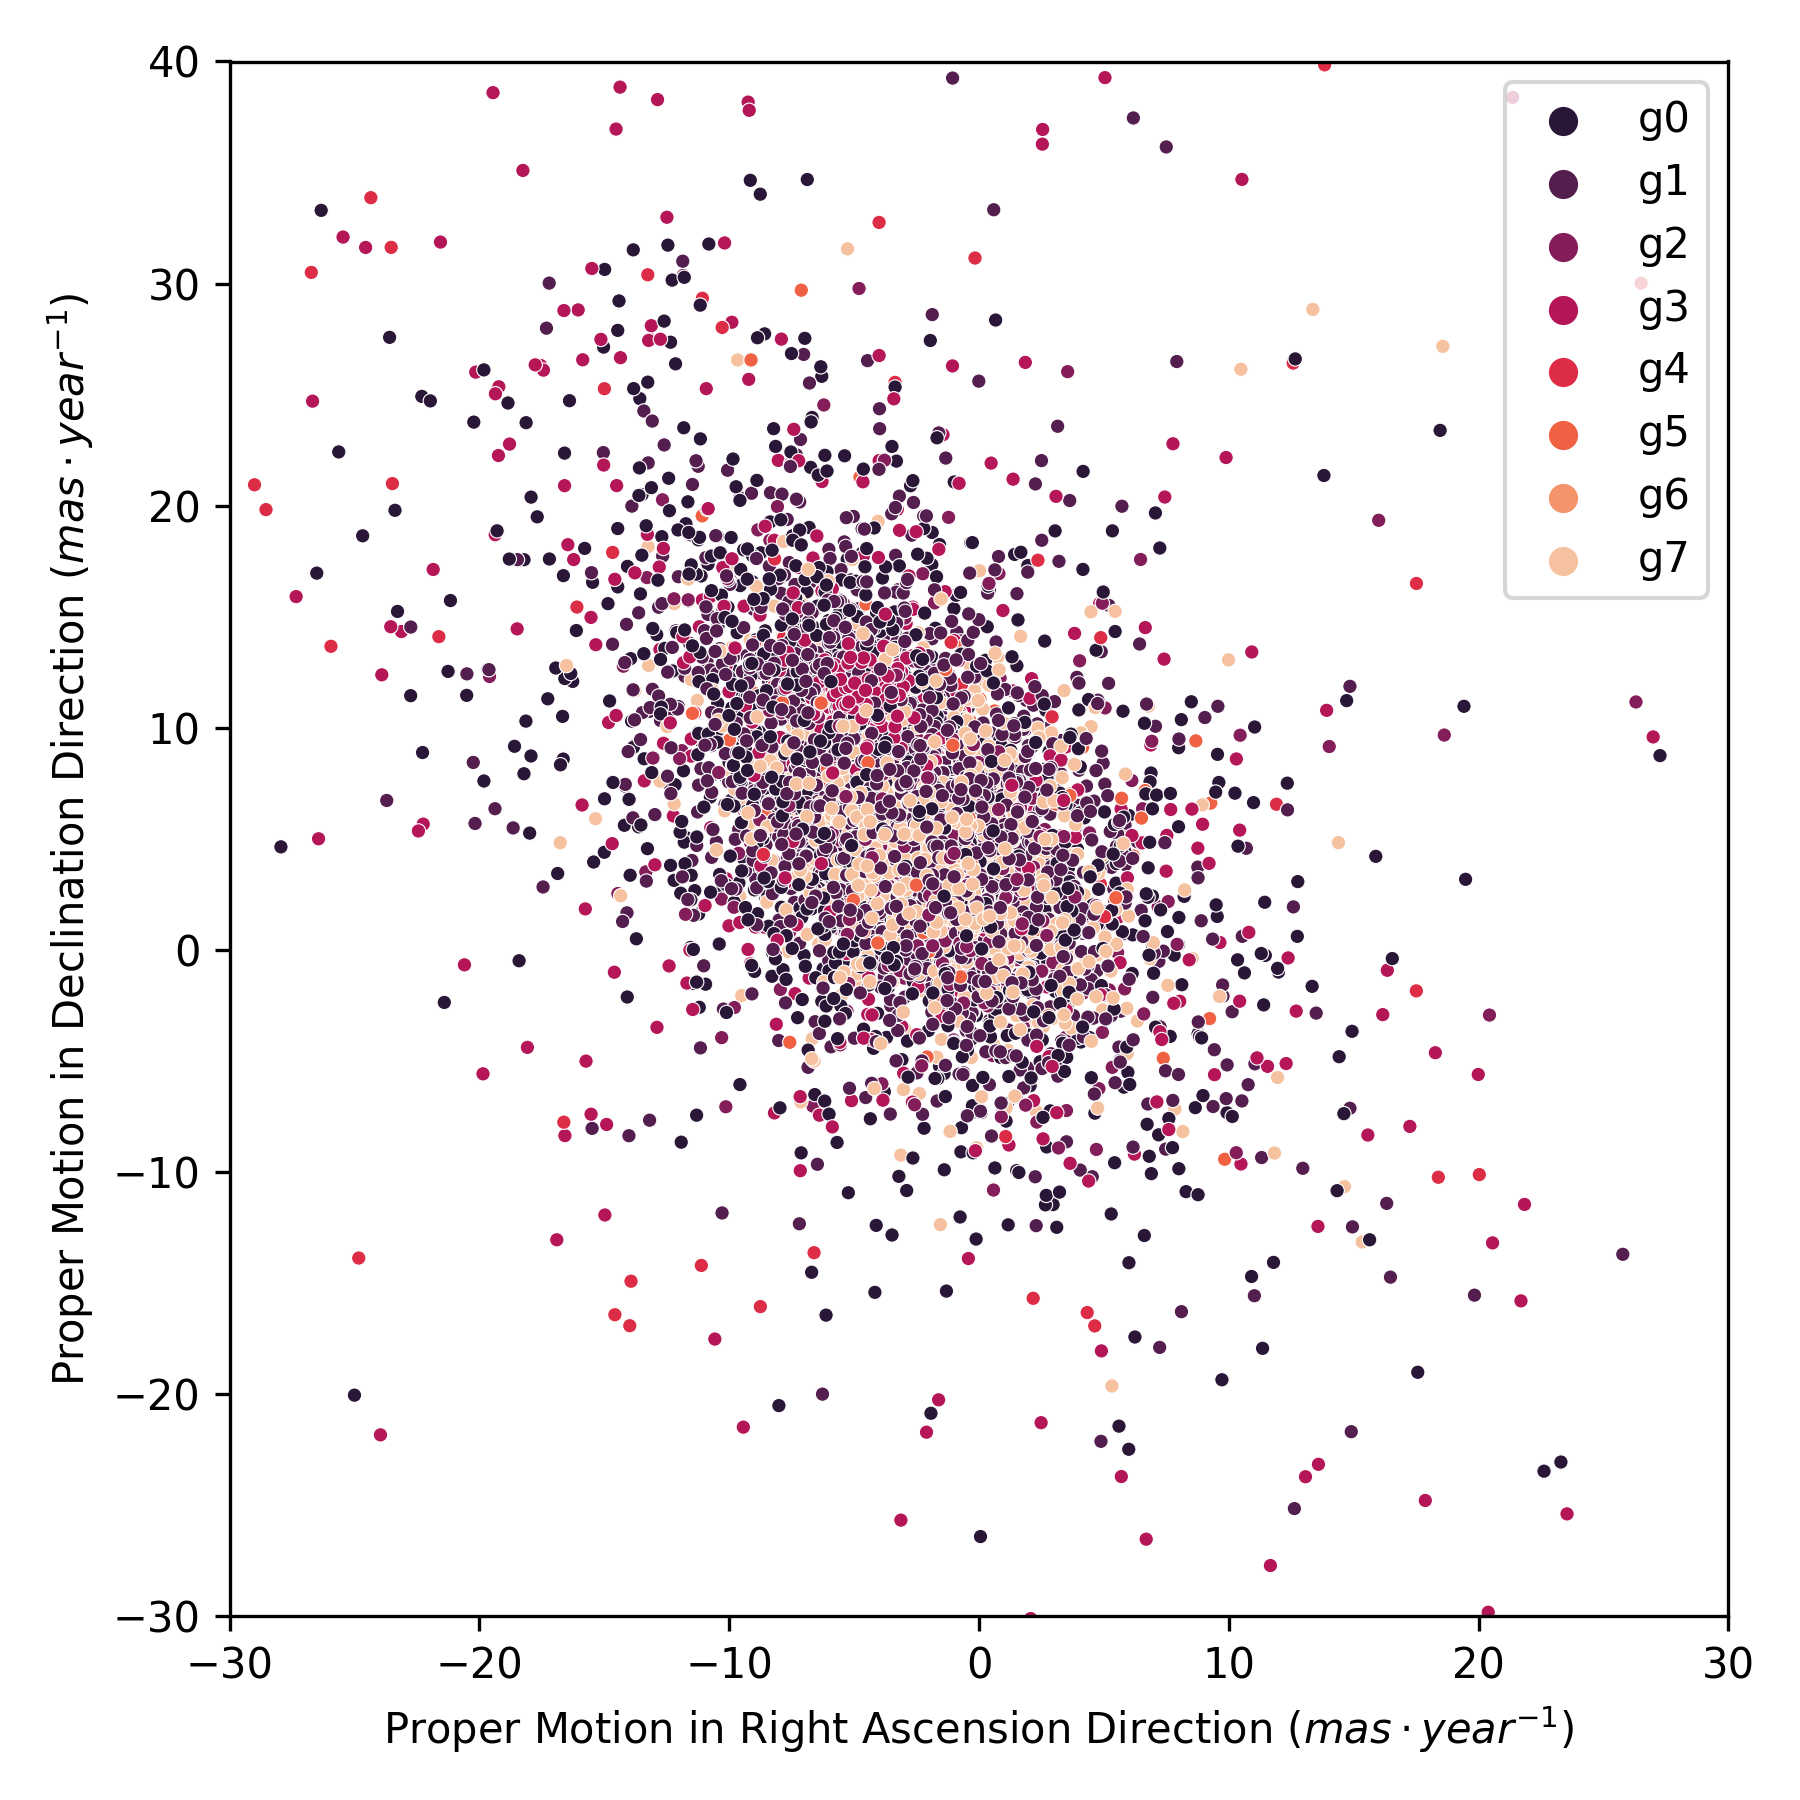
\includegraphics[width=\textwidth]{../figures/ngc_2516/dec_pm_ngc_2516.png}
    \end{subfigure}
    \hfill
    \begin{subfigure}[t]{0.30\textwidth}
      \centering
      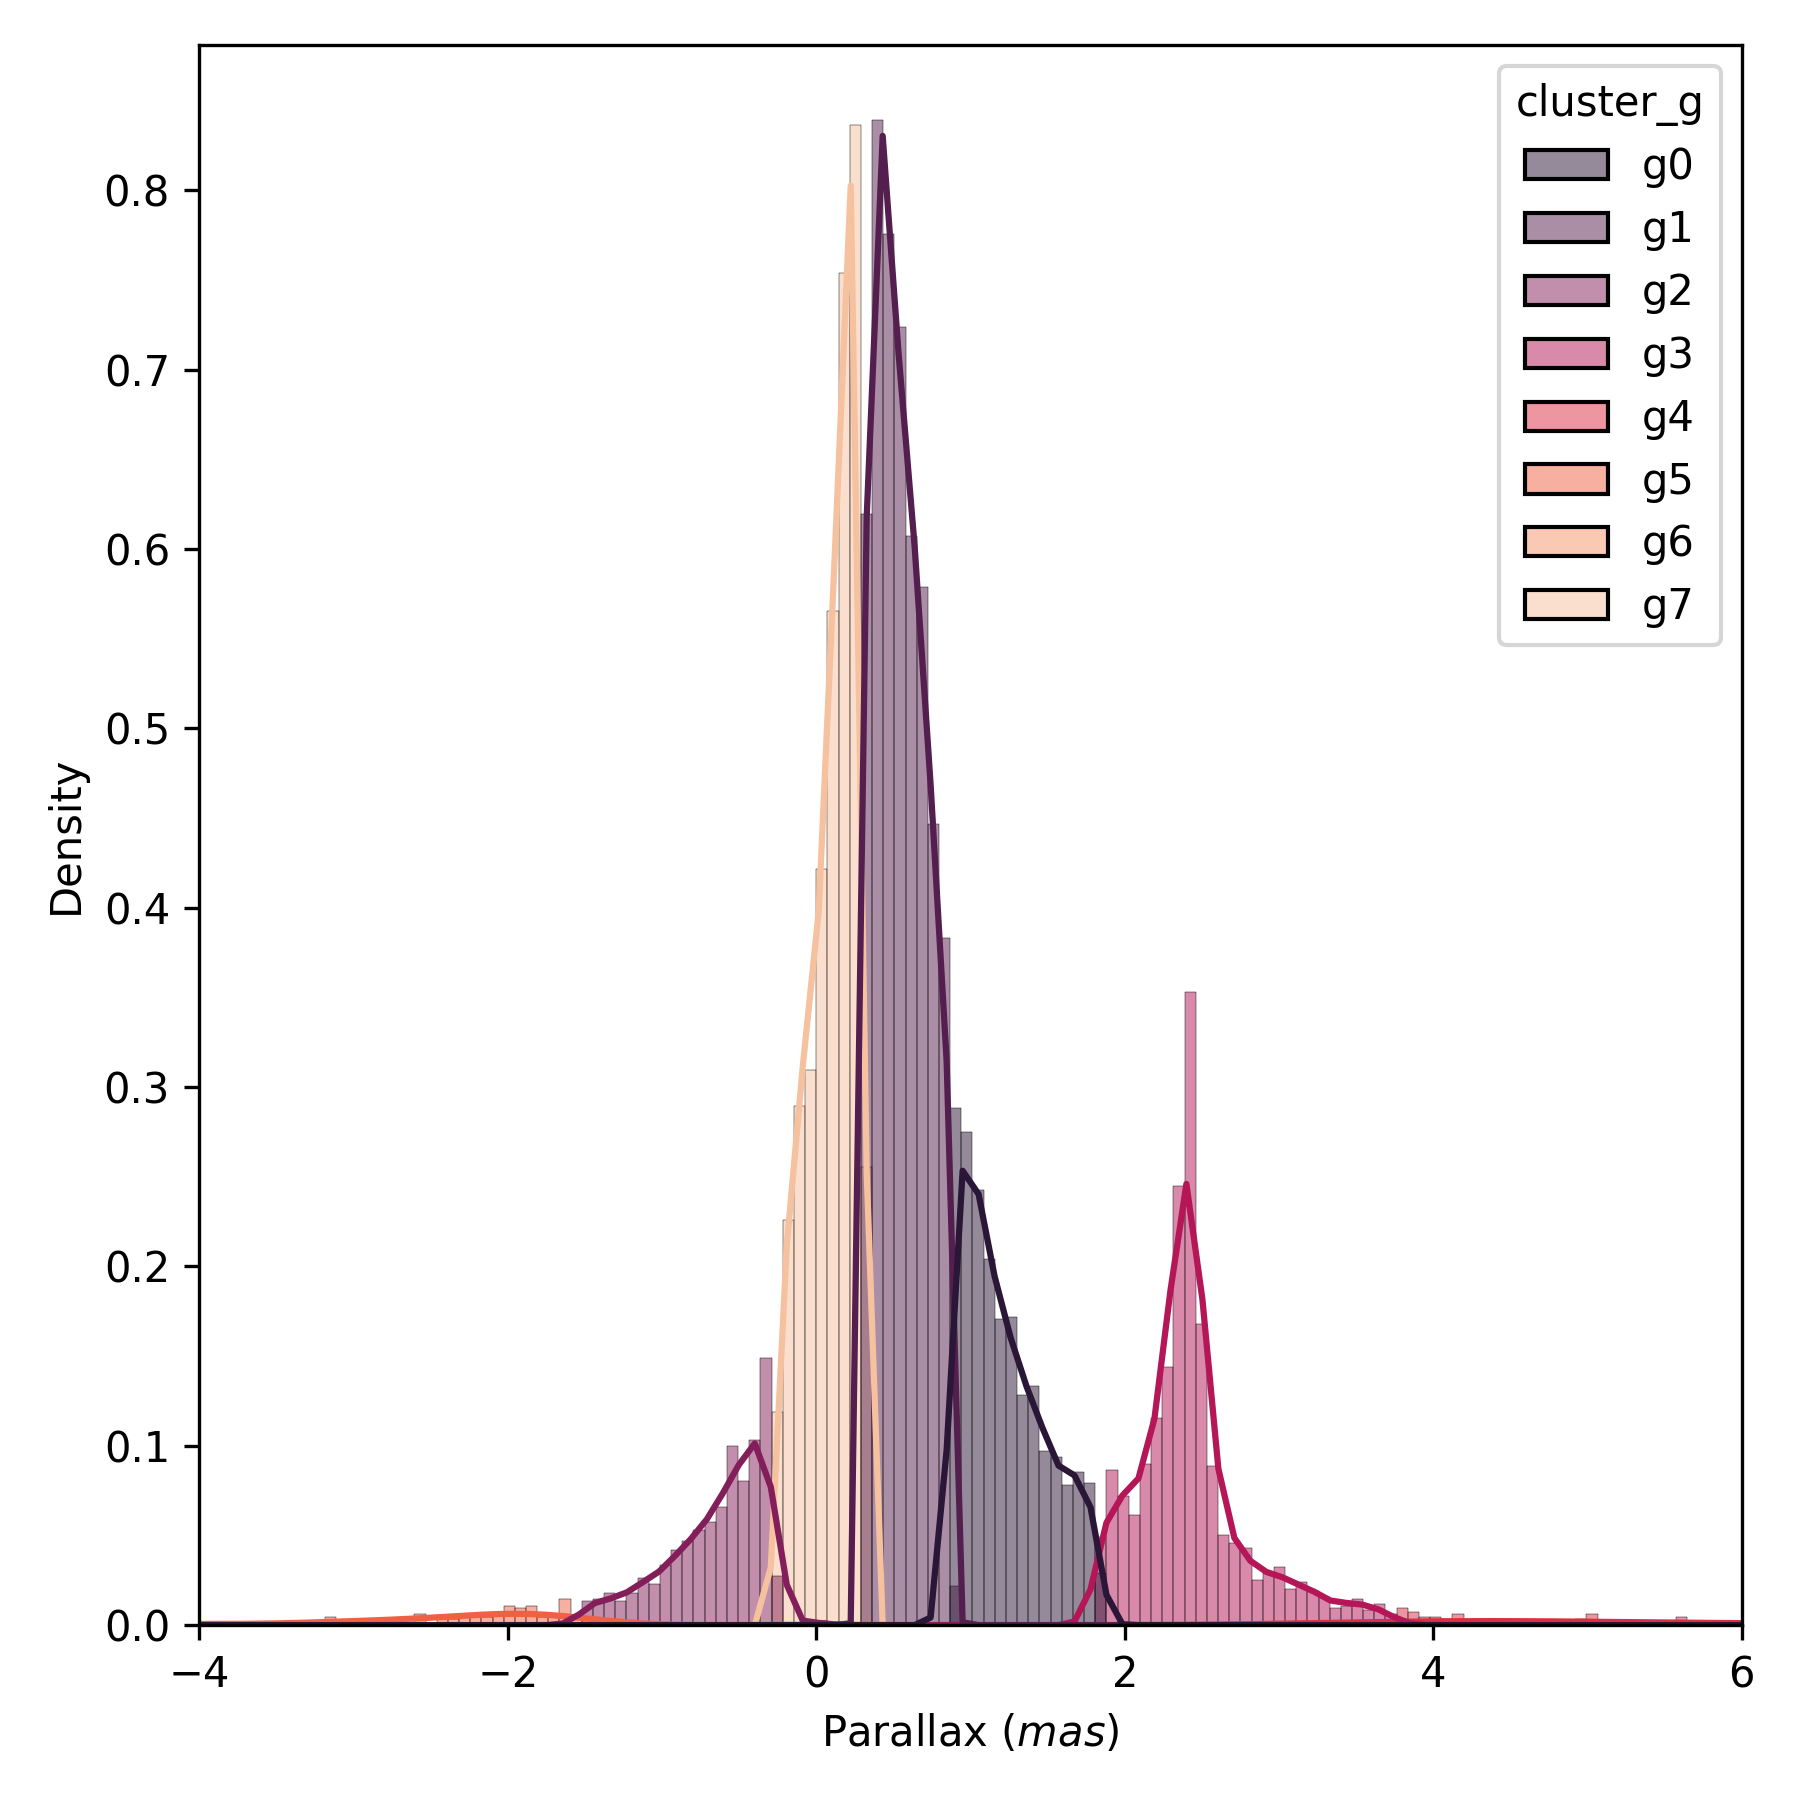
\includegraphics[width=\textwidth]{../figures/ngc_2516/dec_parallax_ngc_2516.png}
    \end{subfigure}
    \hfill
    \begin{subfigure}[t]{0.30\textwidth}
      \centering
      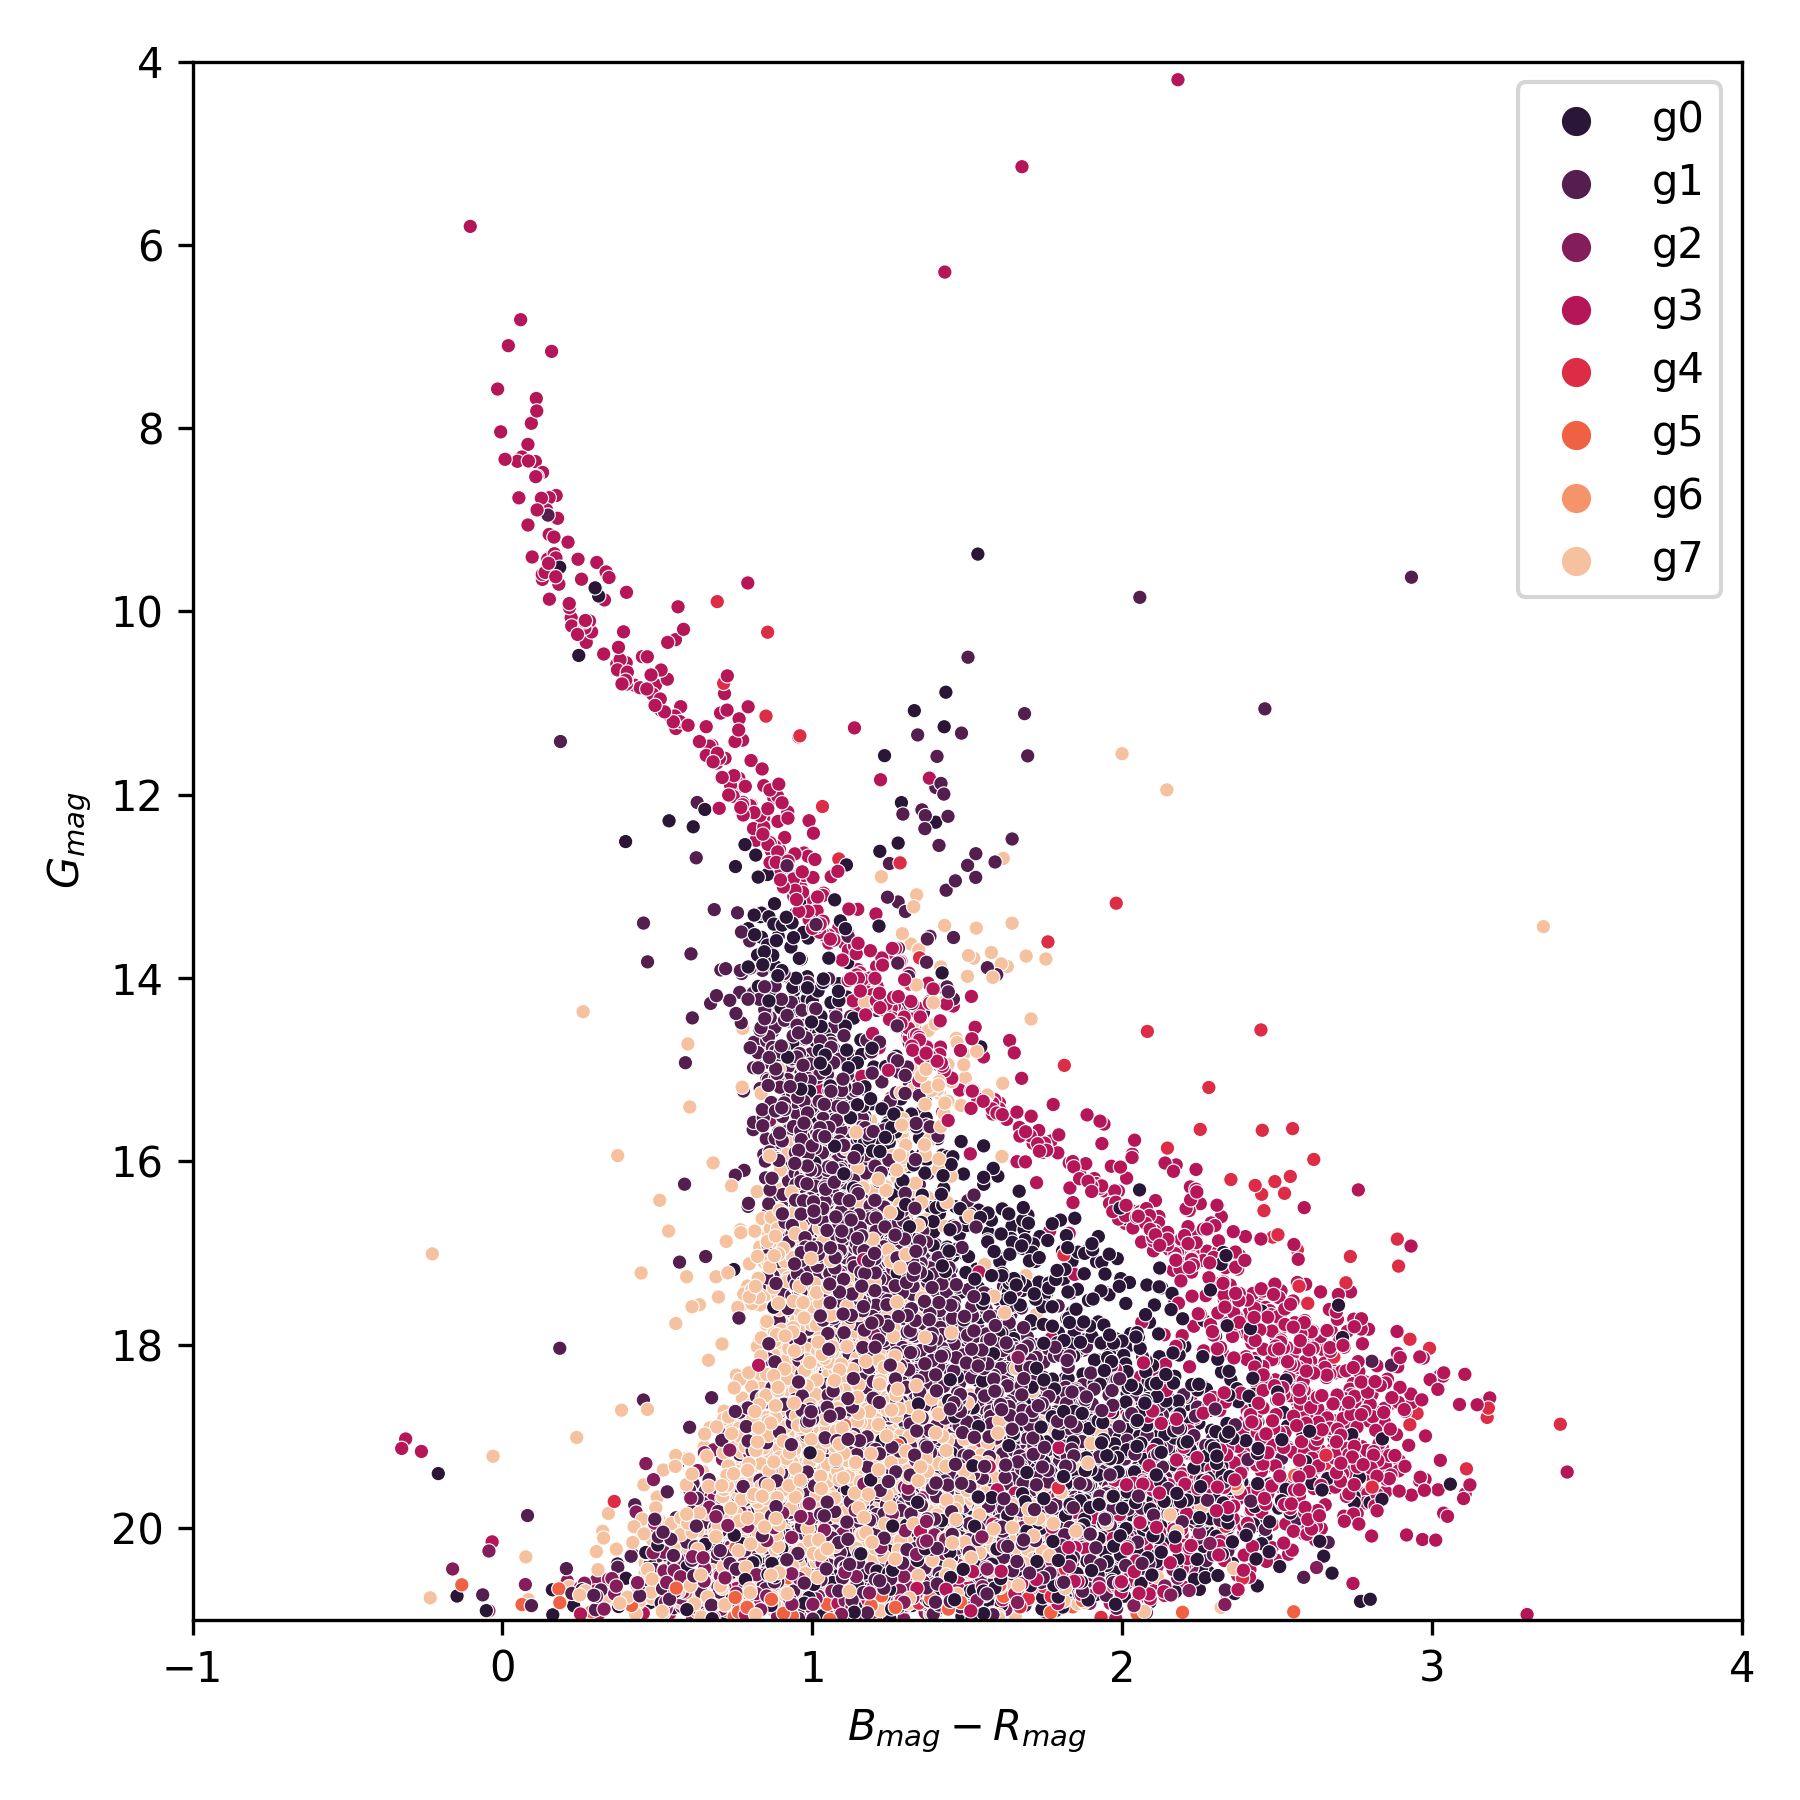
\includegraphics[width=\textwidth]{../figures/ngc_2516/dec_hr_diagram_ngc_2516.png}
    \end{subfigure}
  \end{subfigure}
  \centering
  \begin{subfigure}{\columnwidth}
    \centering
    \begin{subfigure}[t]{0.30\textwidth}
      \centering
      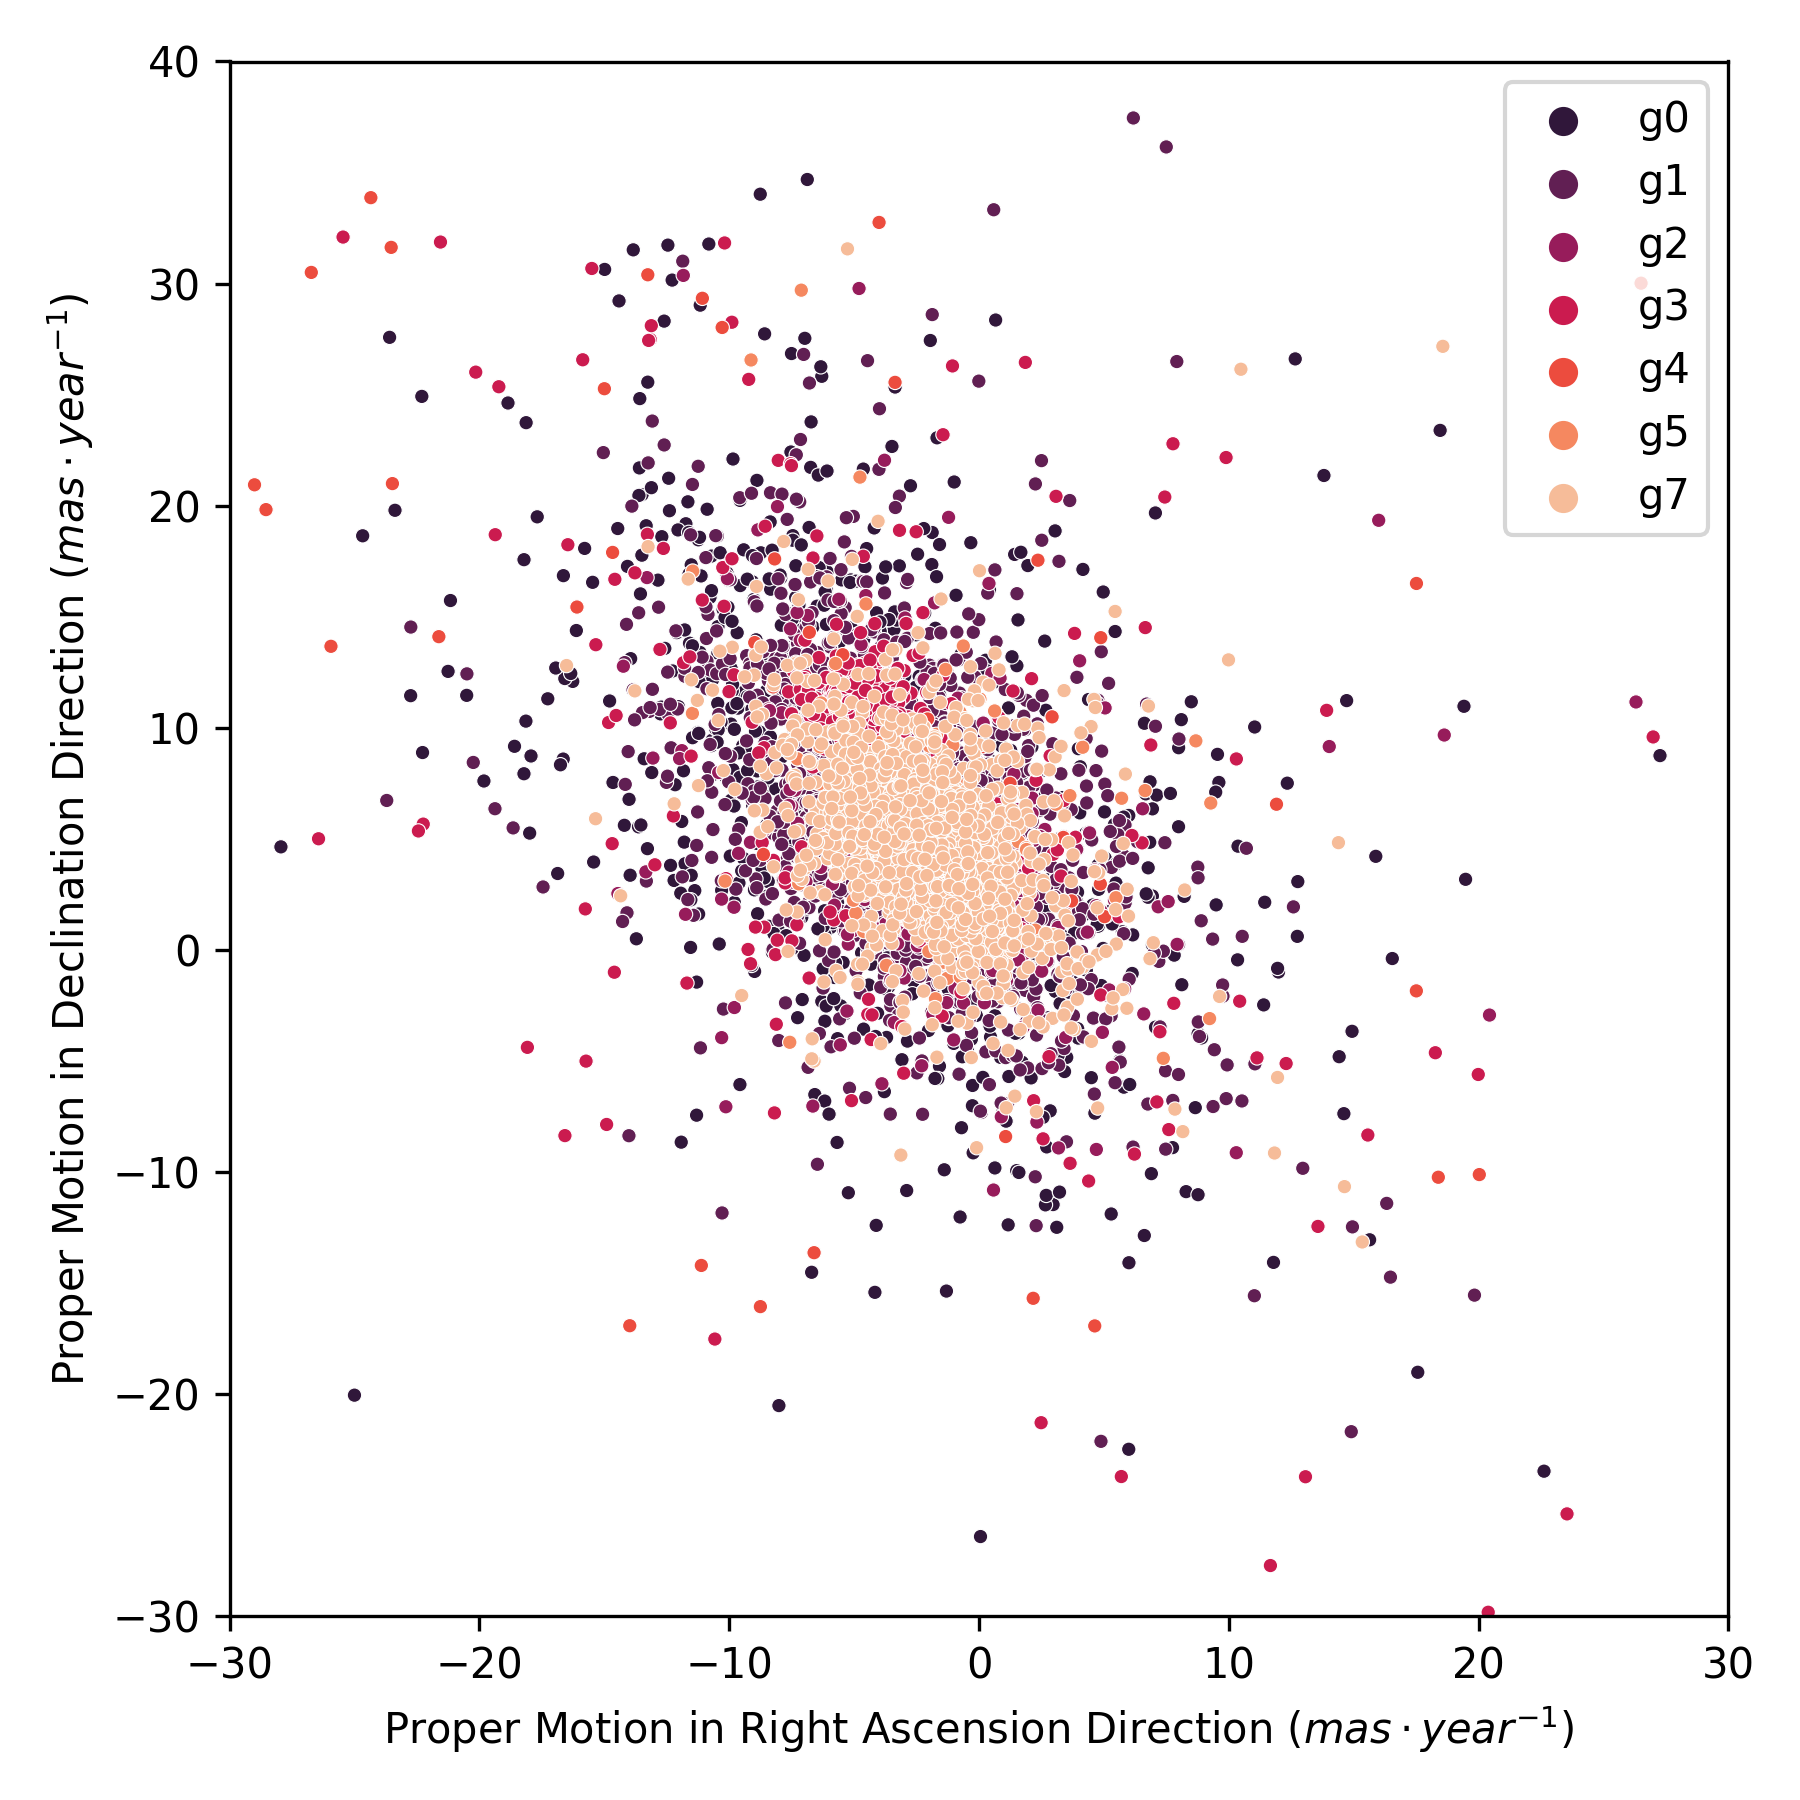
\includegraphics[width=\textwidth]{../figures/ngc_2516/dec_pm_filtered_ngc_2516.png}
    \end{subfigure}
    \hfill
    \begin{subfigure}[t]{0.30\textwidth}
      \centering
      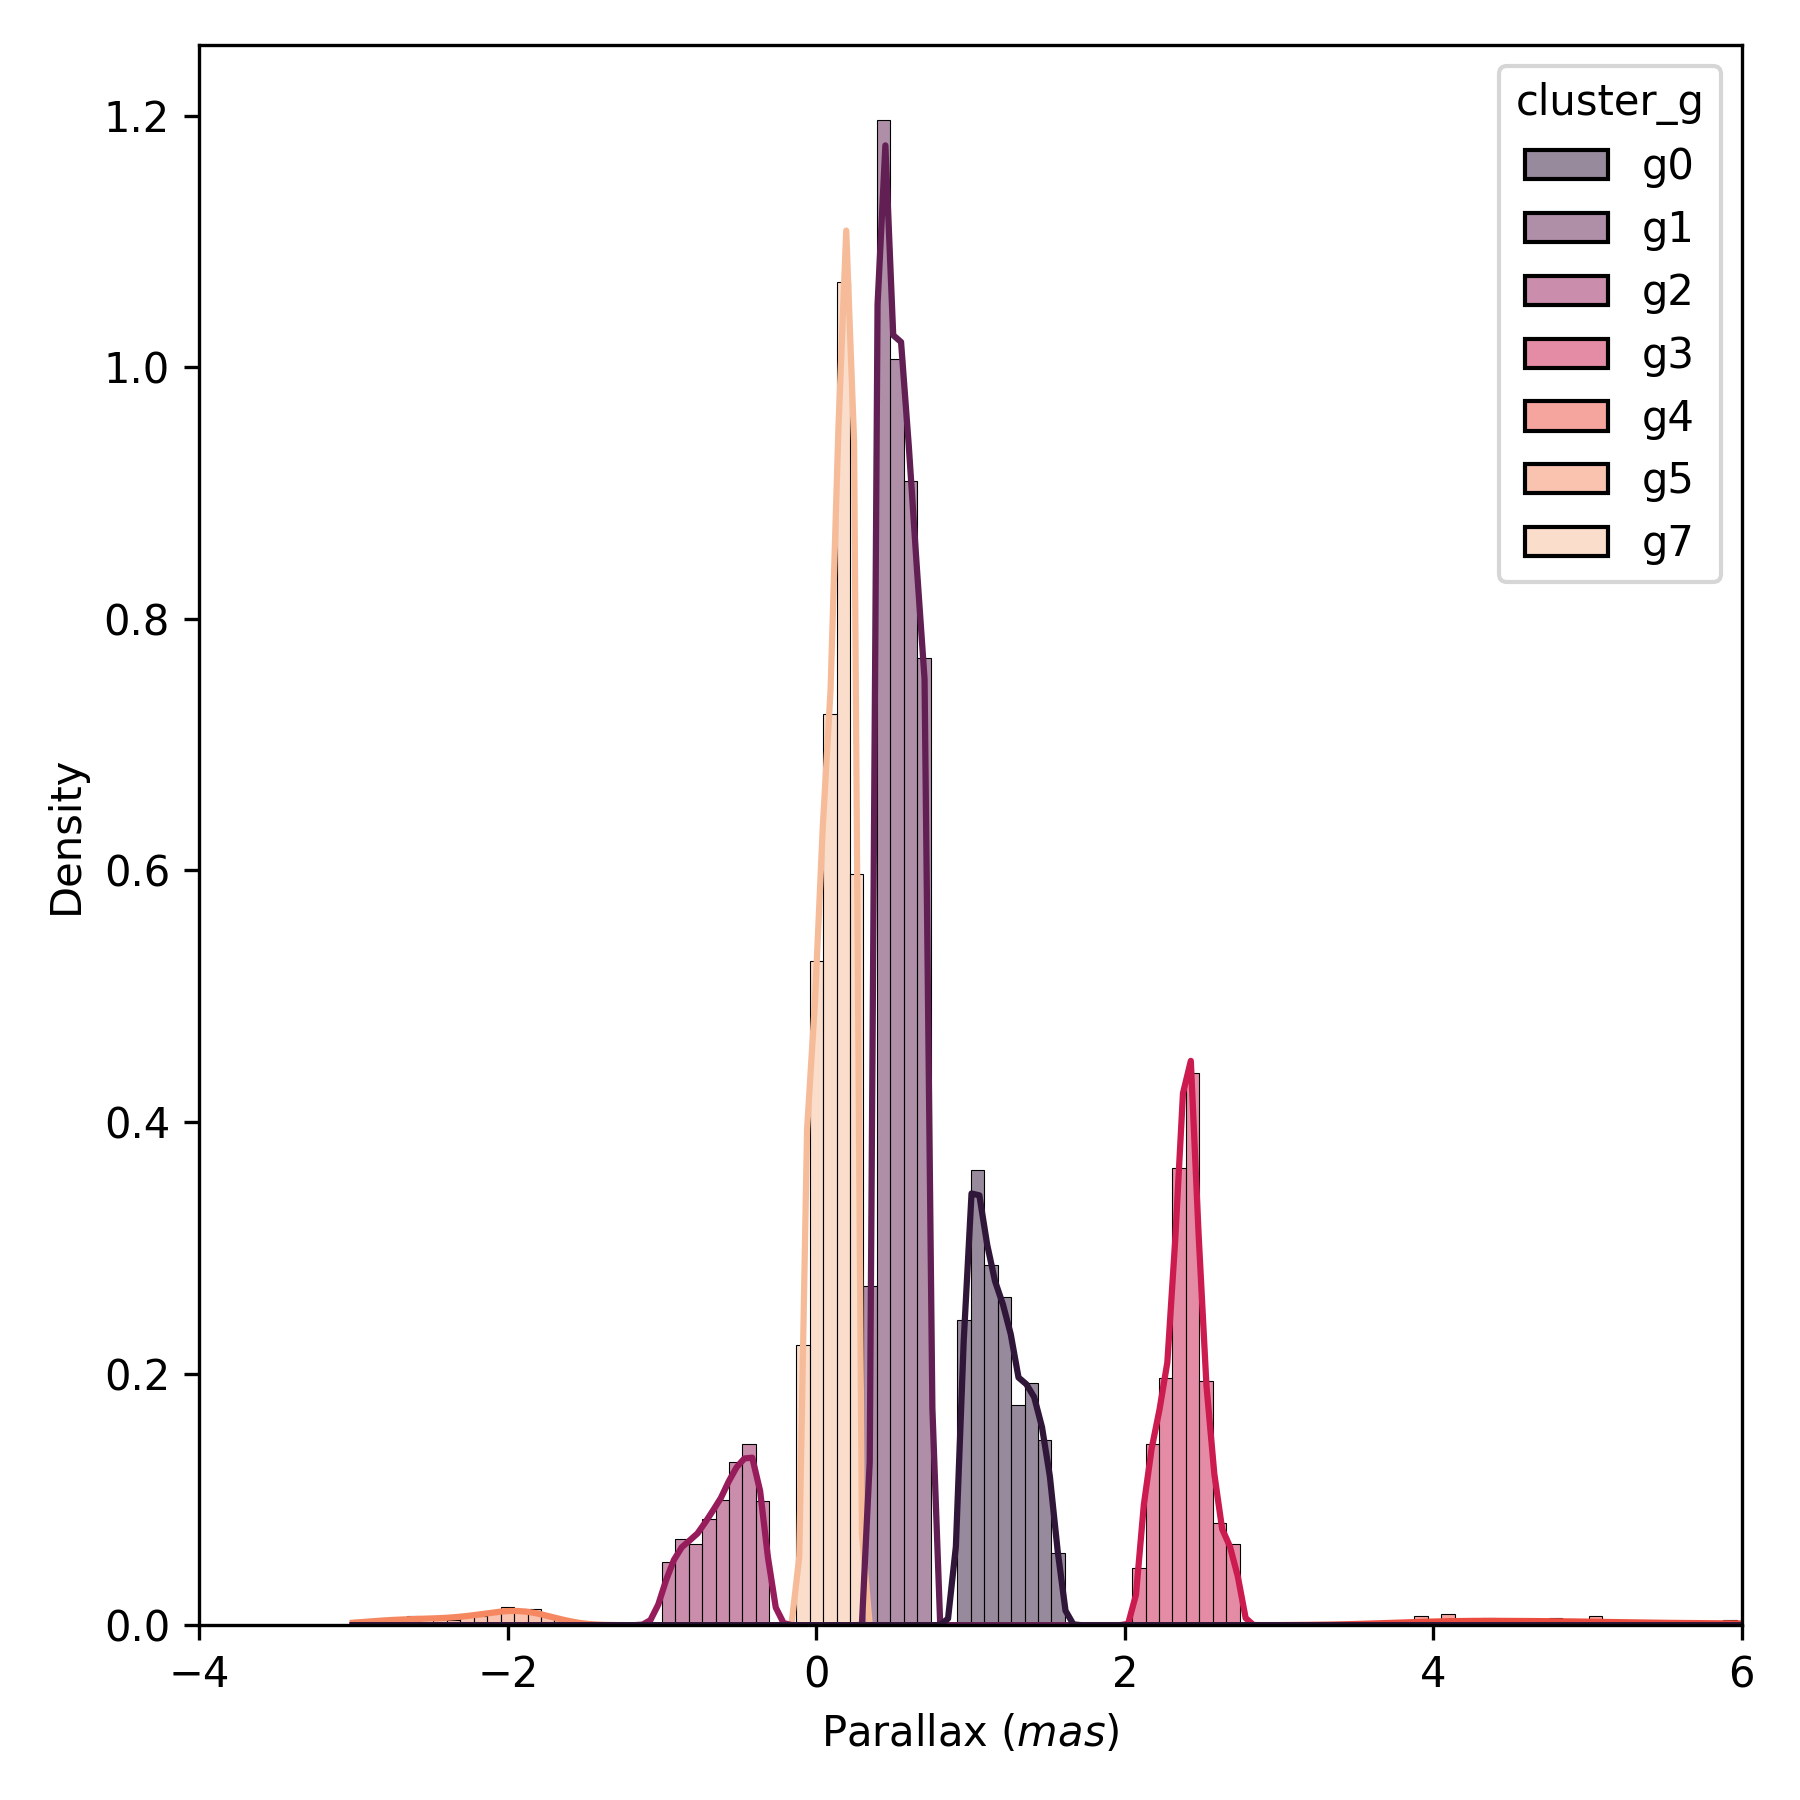
\includegraphics[width=\textwidth]{../figures/ngc_2516/dec_parallax_filtered_ngc_2516.png}
    \end{subfigure}
    \hfill
    \begin{subfigure}[t]{0.30\textwidth}
      \centering
      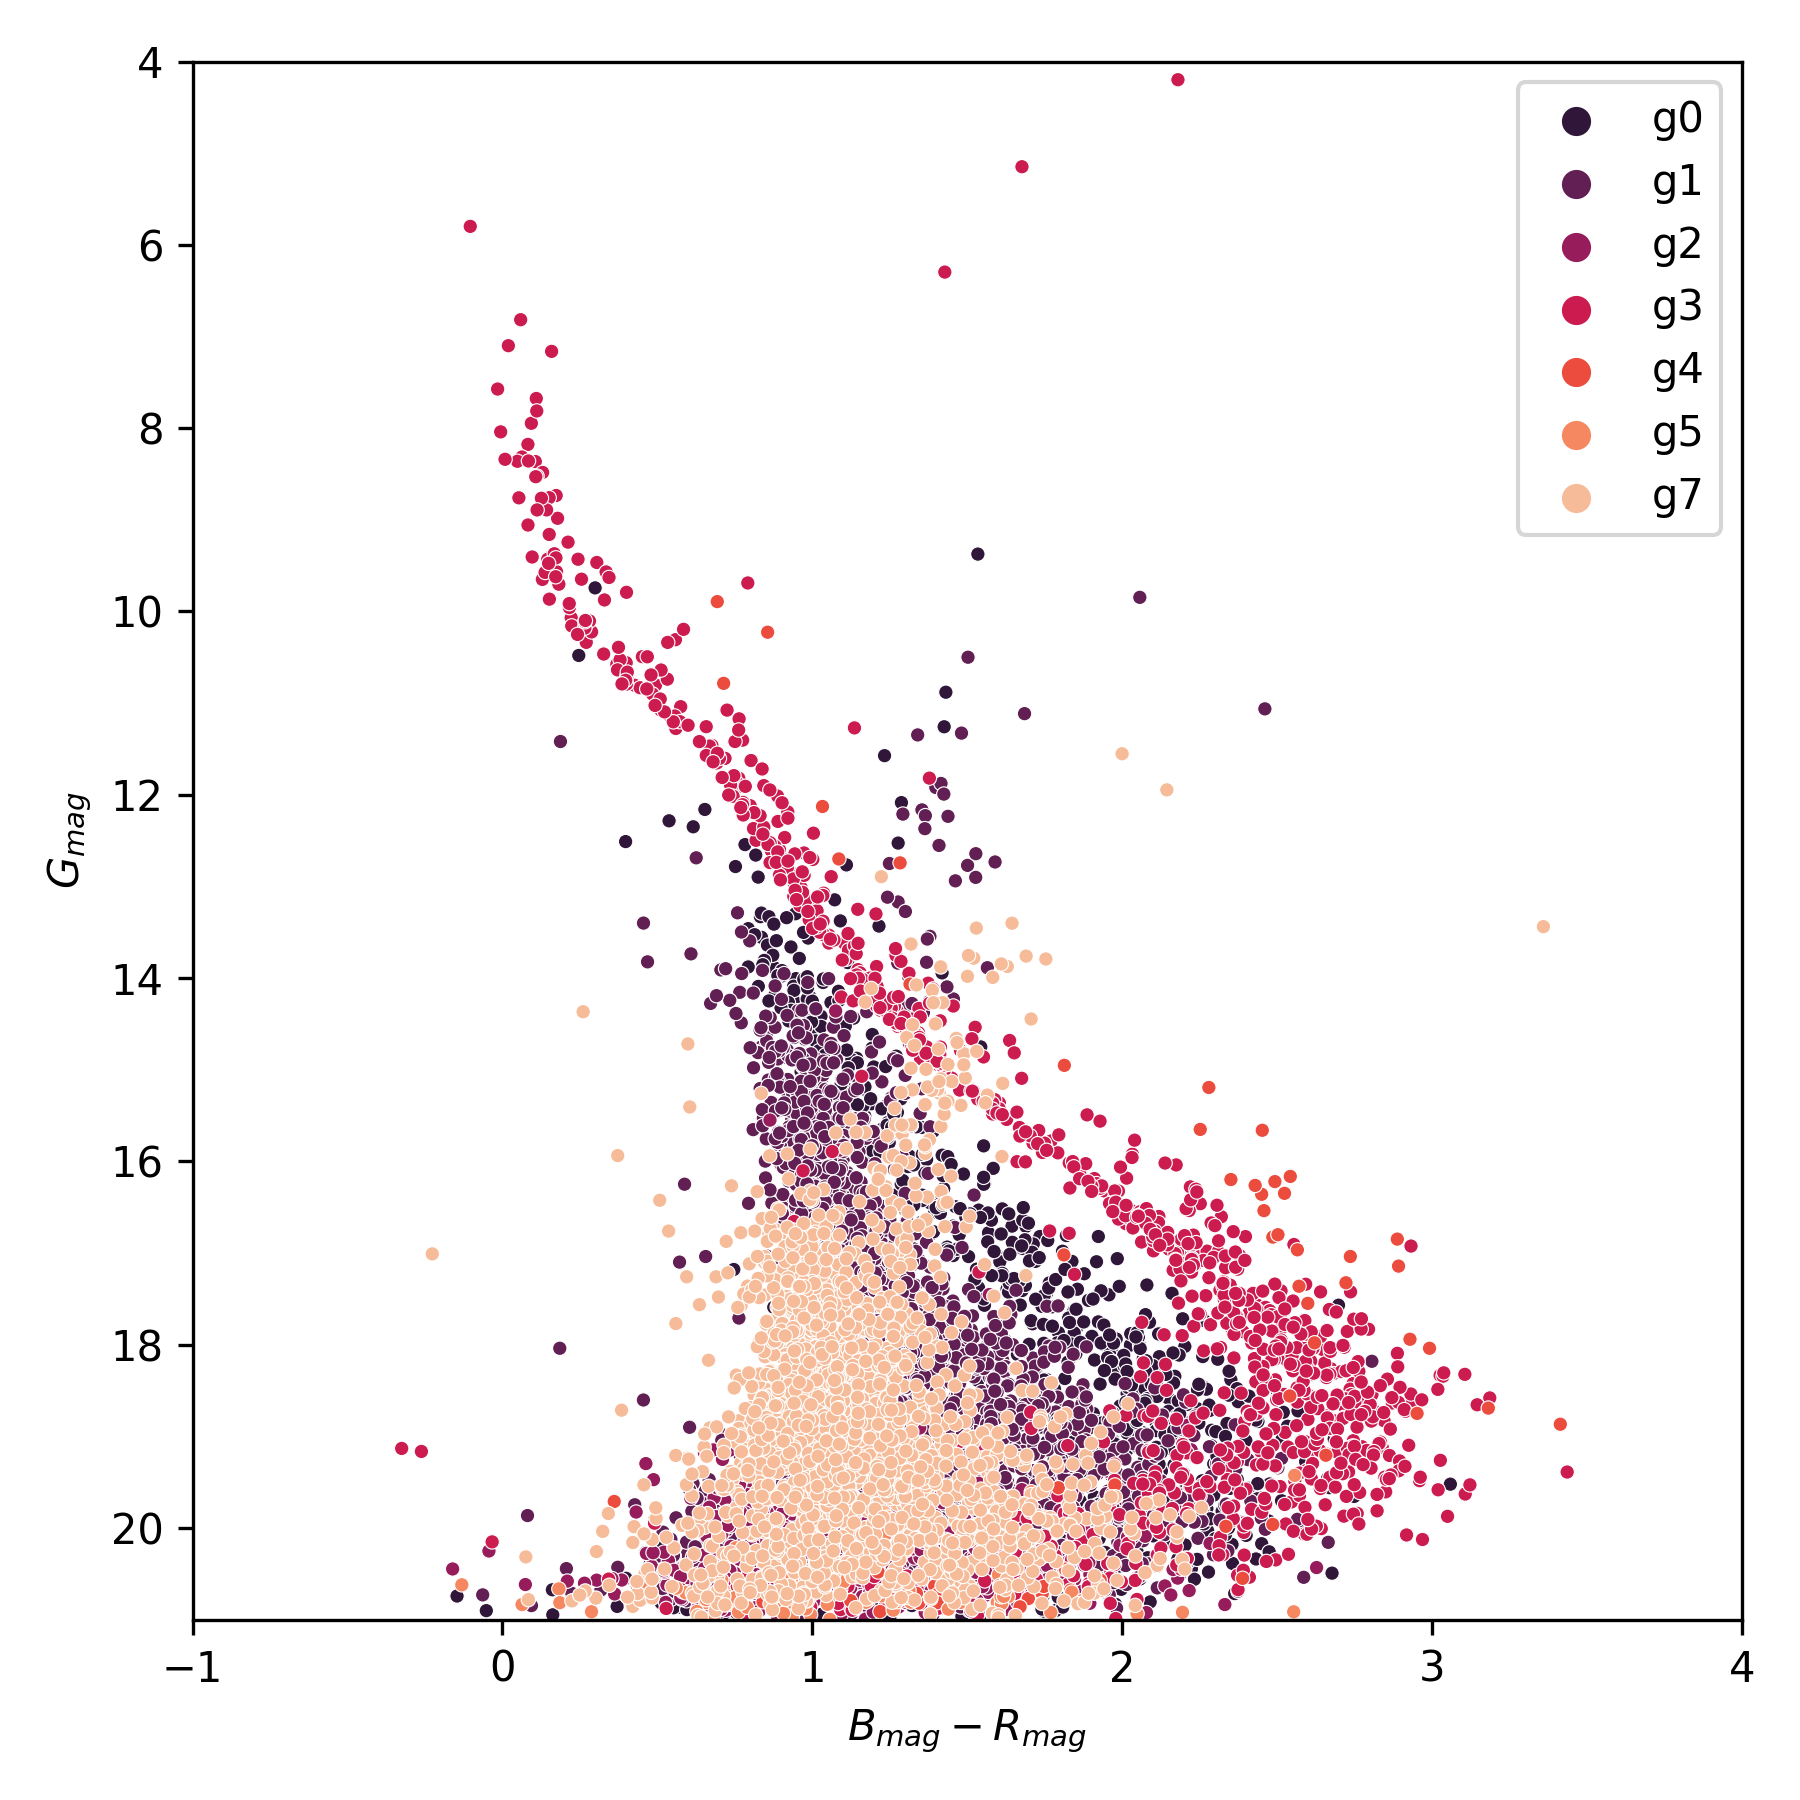
\includegraphics[width=\textwidth]{../figures/ngc_2516/dec_hr_diagram_filtered_ngc_2516.png}
    \end{subfigure}
  \end{subfigure}
  \caption{NGC 2516 characterization (labeled as \emph{g3}).
           DEC (top). DEC filtered (bottom).}
  \label{fig:app_result_ngc_2516_dec}
\end{figure}

\begin{table}[htbp]
  \begin{center}
    \begin{tabular}{l|c}
      \textbf{Hyperparameter} & \textbf{Value} \\
      \hline
      Number of Clusters & 8 \\
      Clustering Layer & $\left[ 50, 50, 60 \right]$ \\
      Kernel Initializer Seed & 2 \\
      Quantil Threshold & 0.15 \\
    \end{tabular}
    \caption{NGC 2516 DEC hyperparameters.}
    \label{tab:app_hyperparameters_ngc_2516}
  \end{center}
\end{table}

\subsection{NGC 2632}
\label{sec:ngc2632}

Figure \ref{fig:app_result_ngc_2632_clusterix_kmeans} shows NGC 2632 characterized
by the validation method (first row) and the characterization made by K-Means
showing ten clusters (second row). K-Means labels NGC 2632 as \emph{g1}.

\begin{figure}[htbp]
  \centering
  \begin{subfigure}{\columnwidth}
    \centering
    \begin{subfigure}[t]{0.30\textwidth}
      \centering
      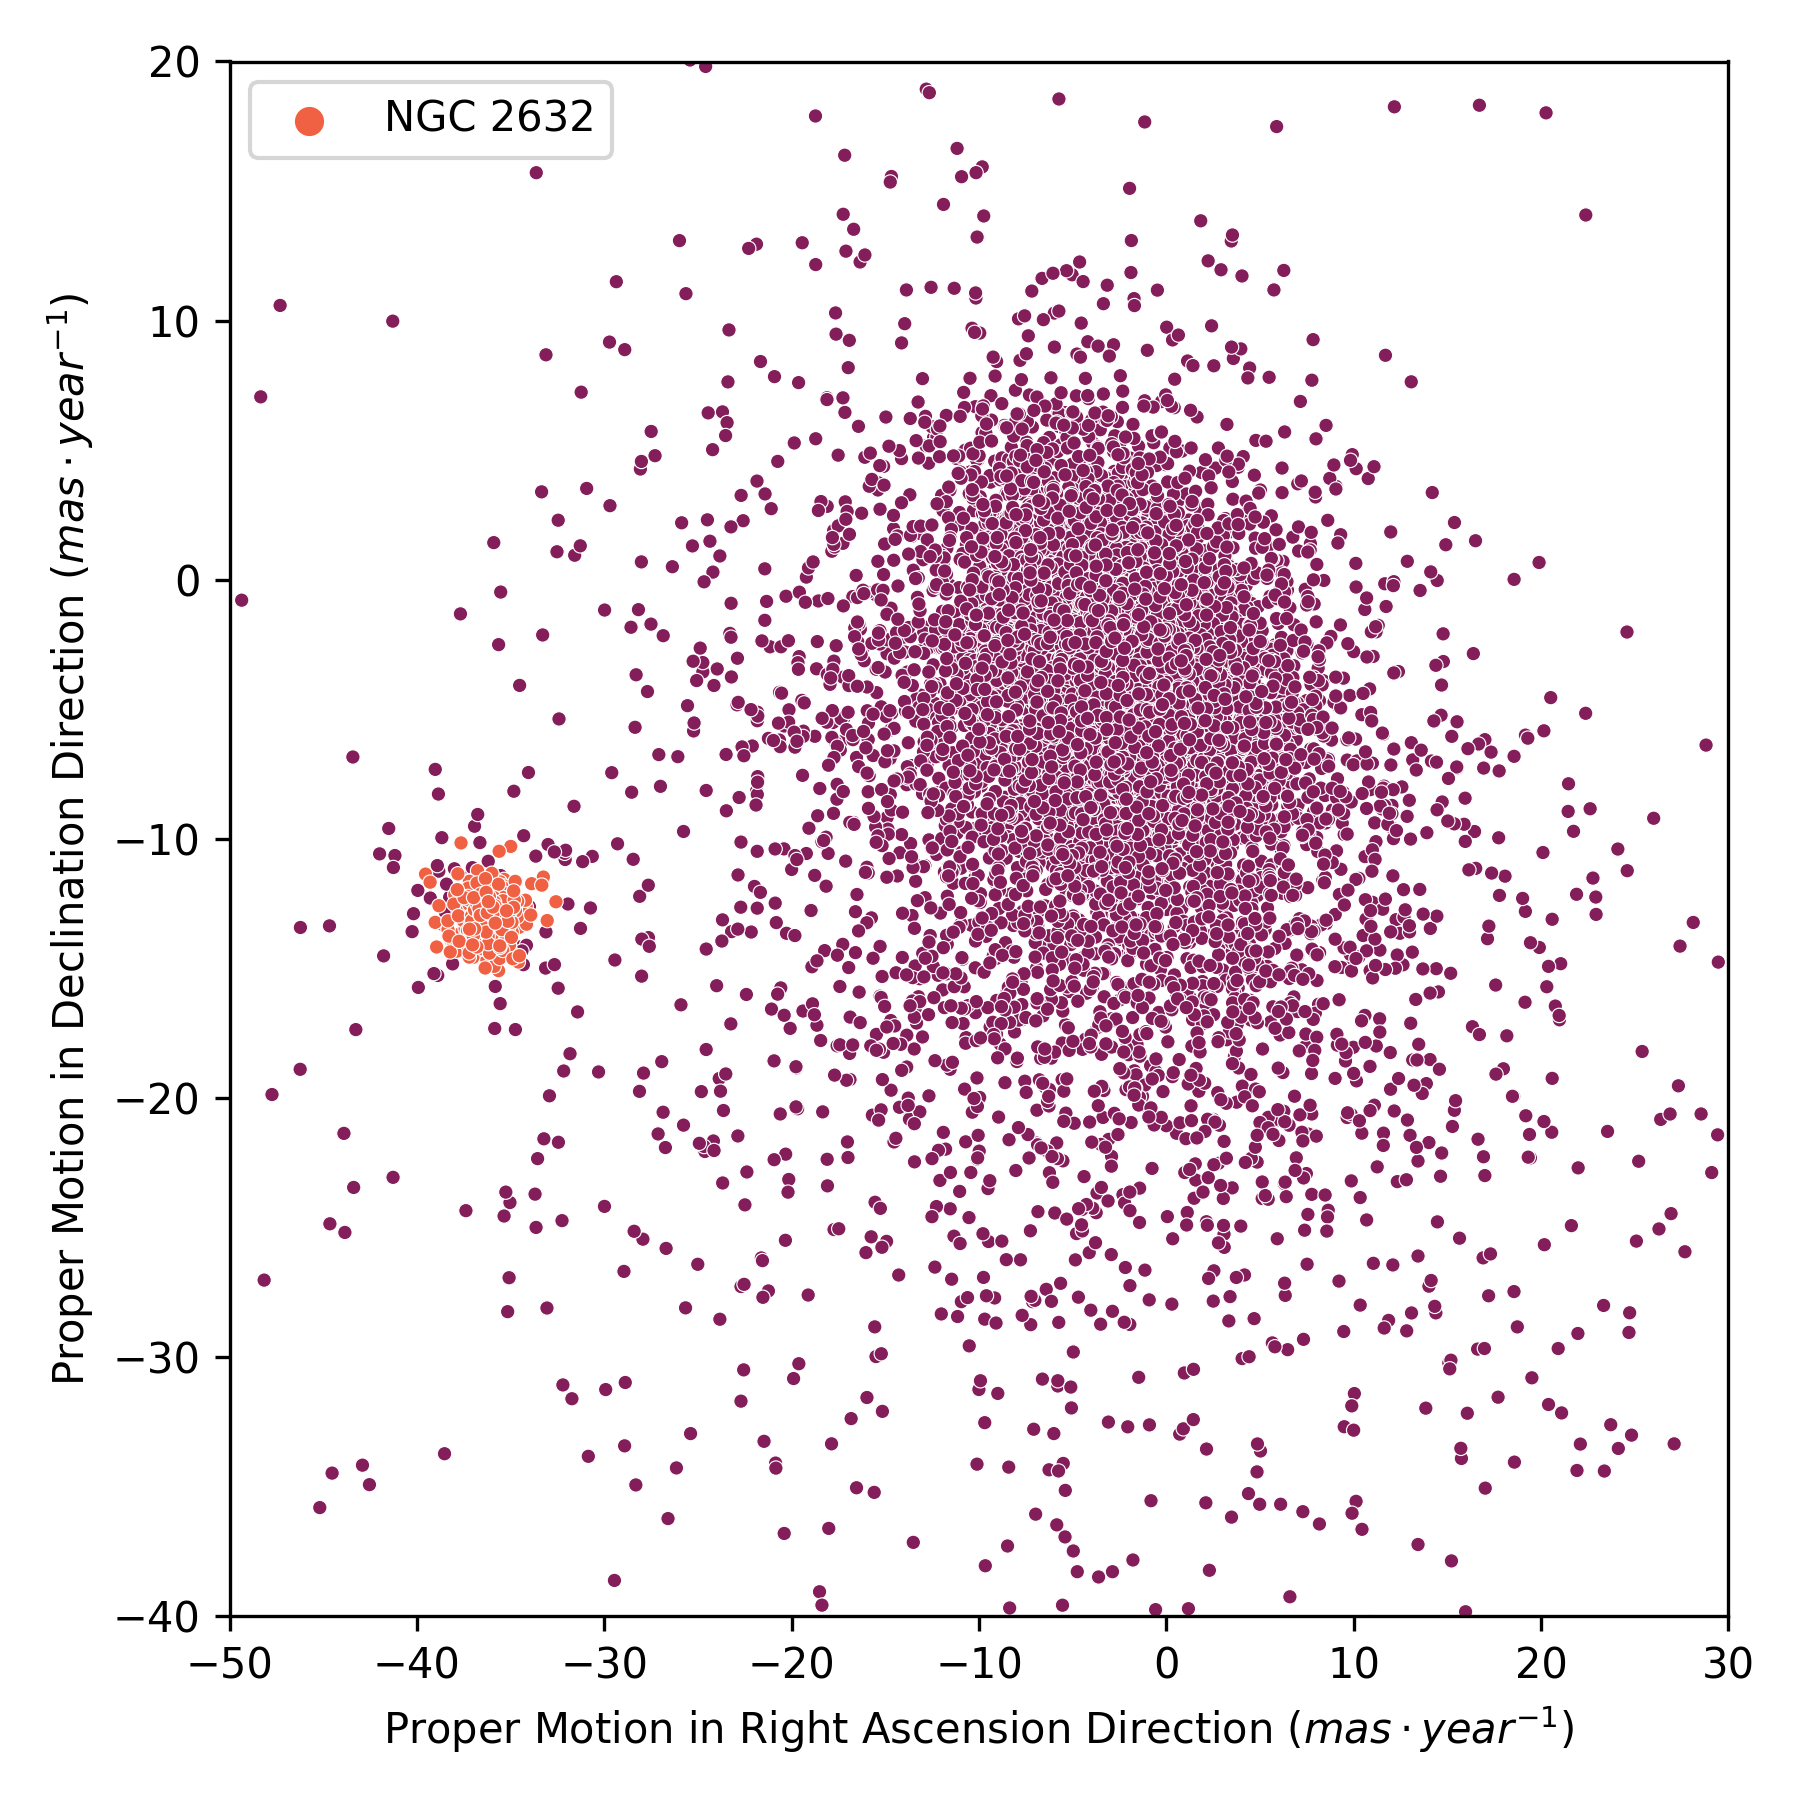
\includegraphics[width=\textwidth]{../figures/ngc_2632/pm_ngc_2632.png}
    \end{subfigure}
    \hfill
    \begin{subfigure}[t]{0.30\textwidth}
      \centering
      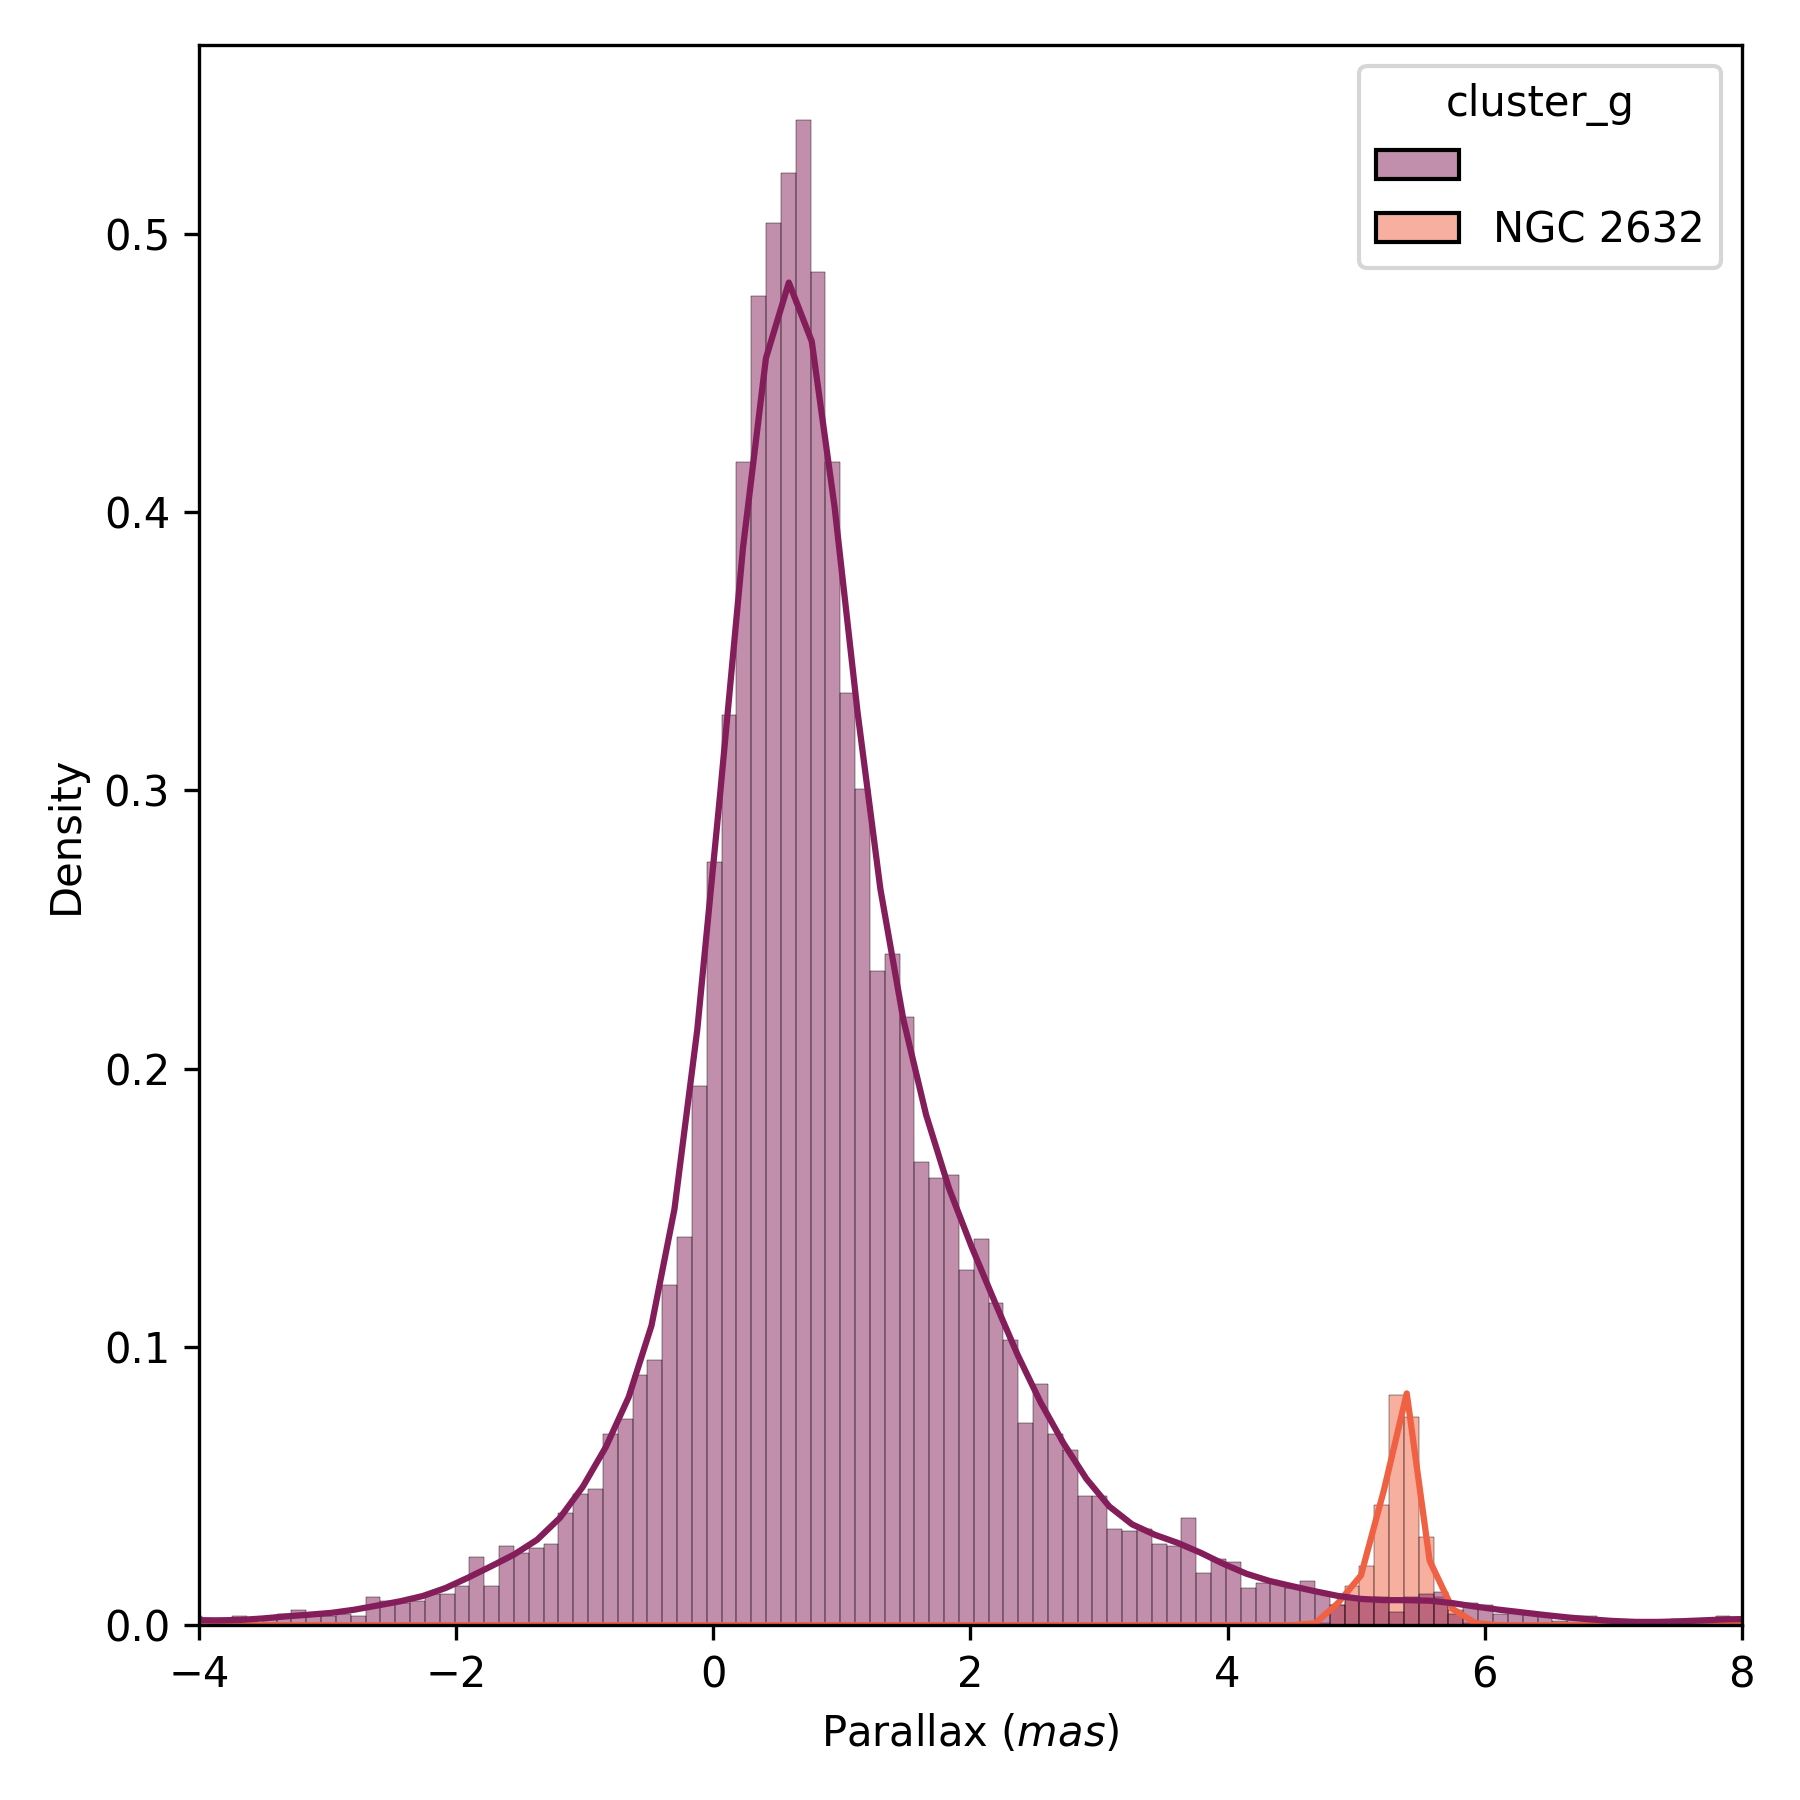
\includegraphics[width=\textwidth]{../figures/ngc_2632/parallax_ngc_2632.png}
    \end{subfigure}
    \hfill
    \begin{subfigure}[t]{0.30\textwidth}
      \centering
      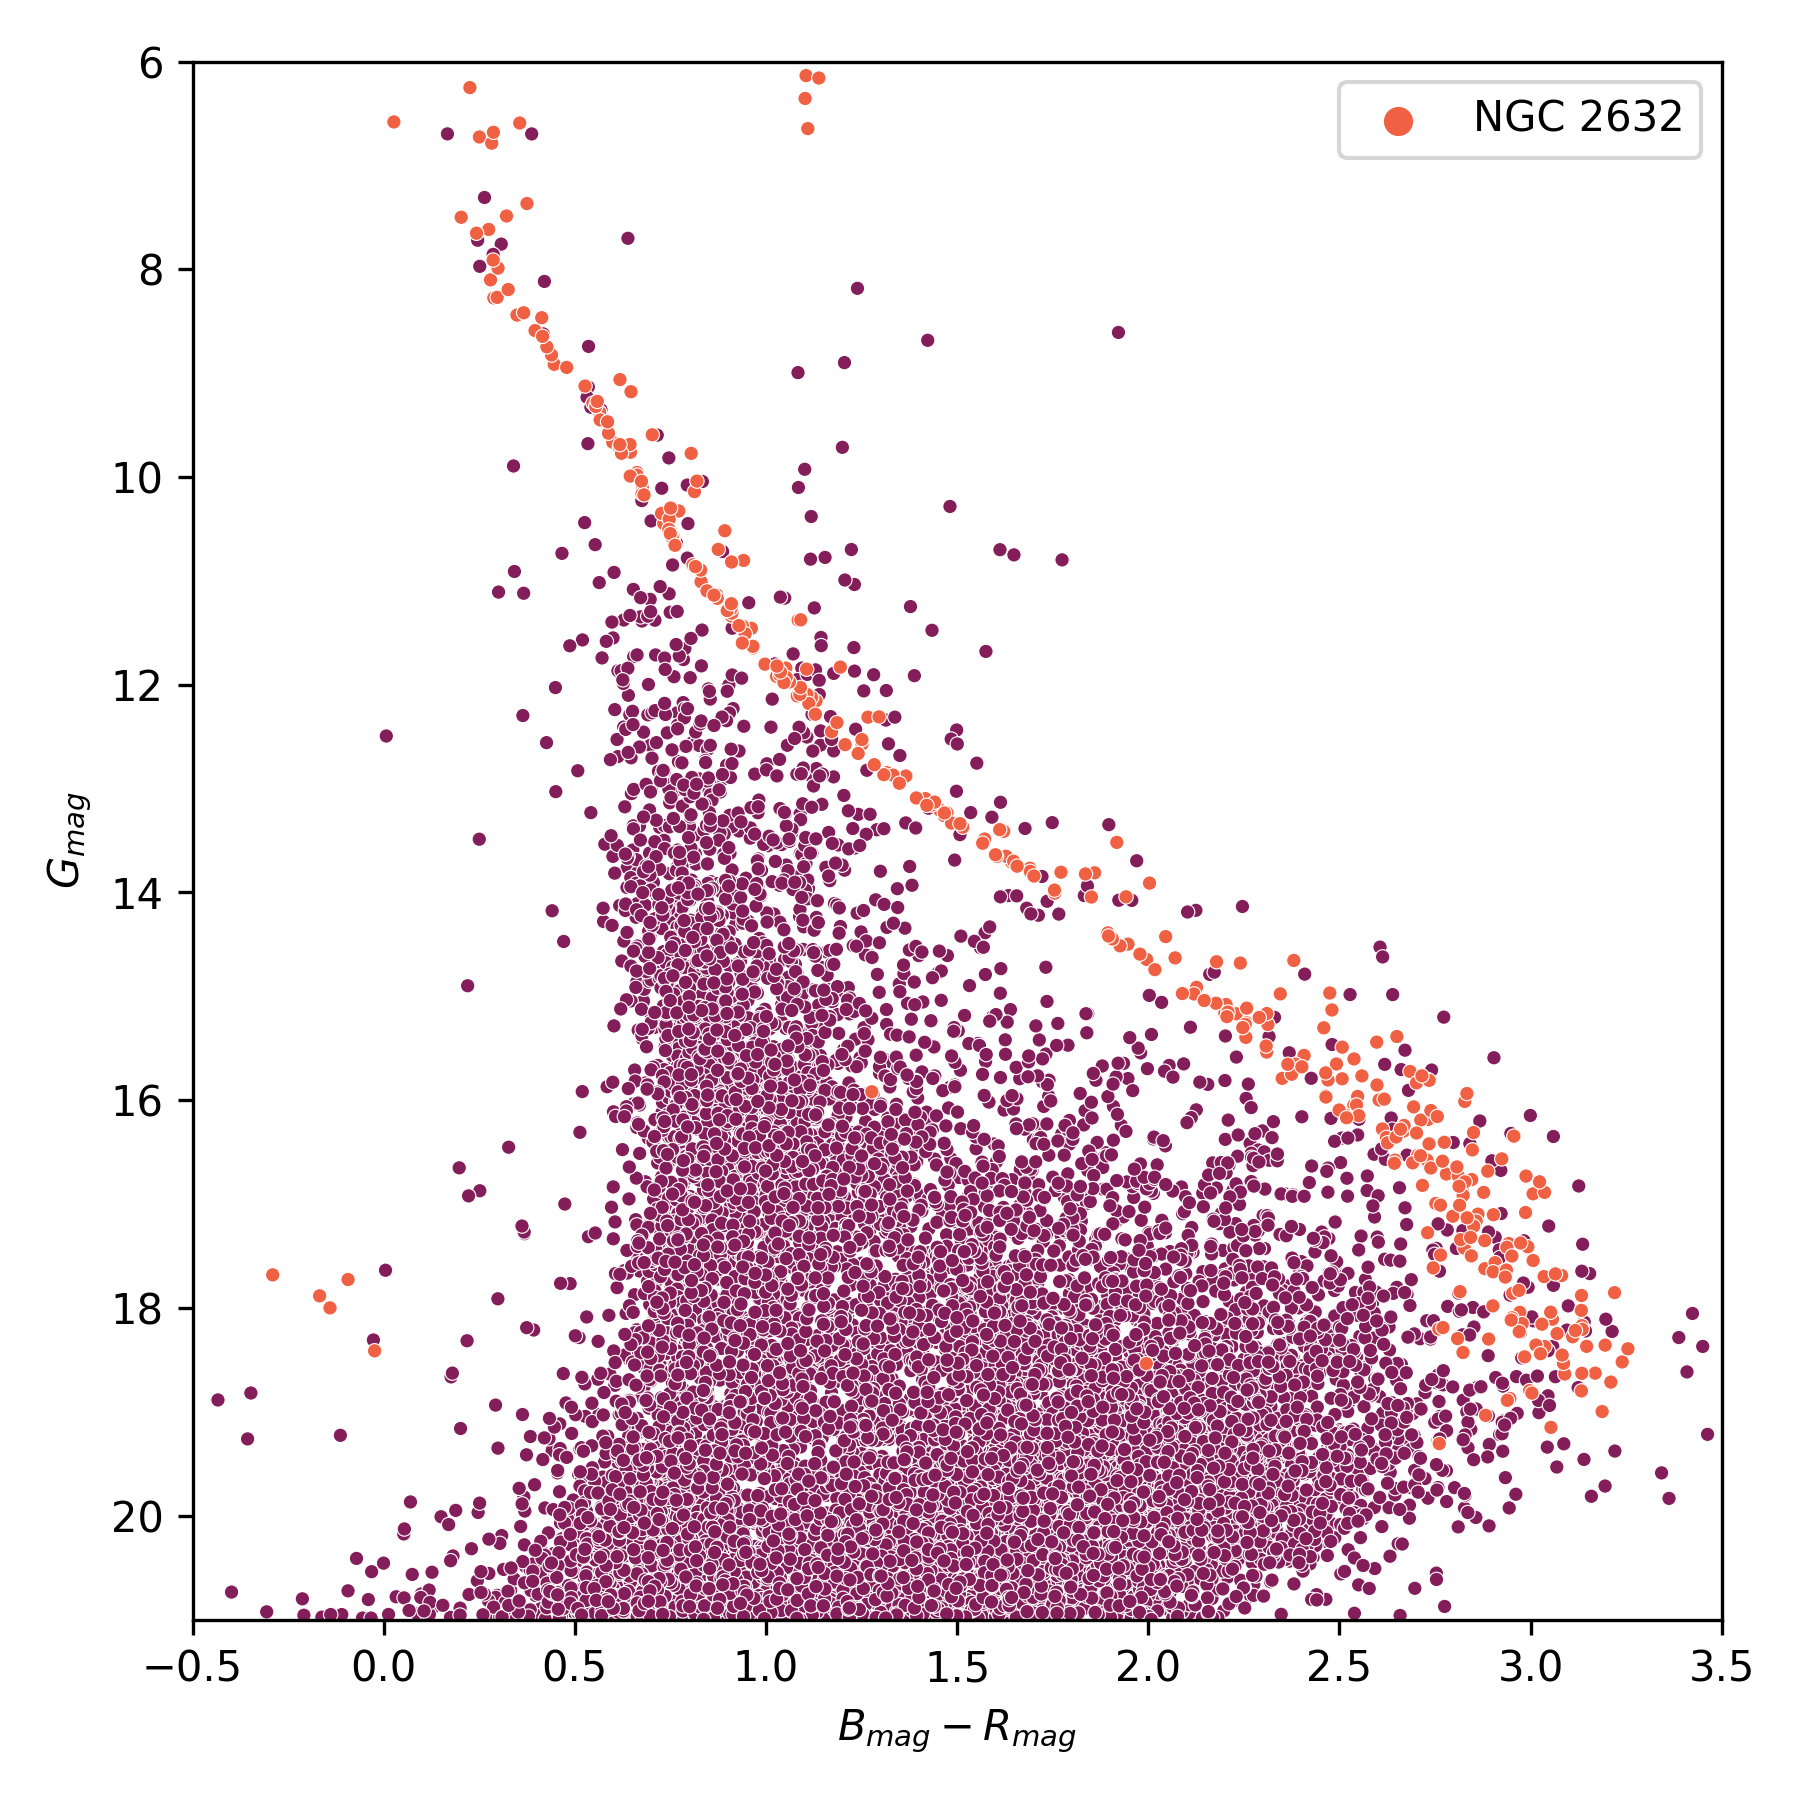
\includegraphics[width=\textwidth]{../figures/ngc_2632/hr_diagram_ngc_2632.png}
    \end{subfigure}
  \end{subfigure}
  \centering
  \begin{subfigure}{\columnwidth}
    \centering
    \begin{subfigure}[t]{0.30\textwidth}
      \centering
      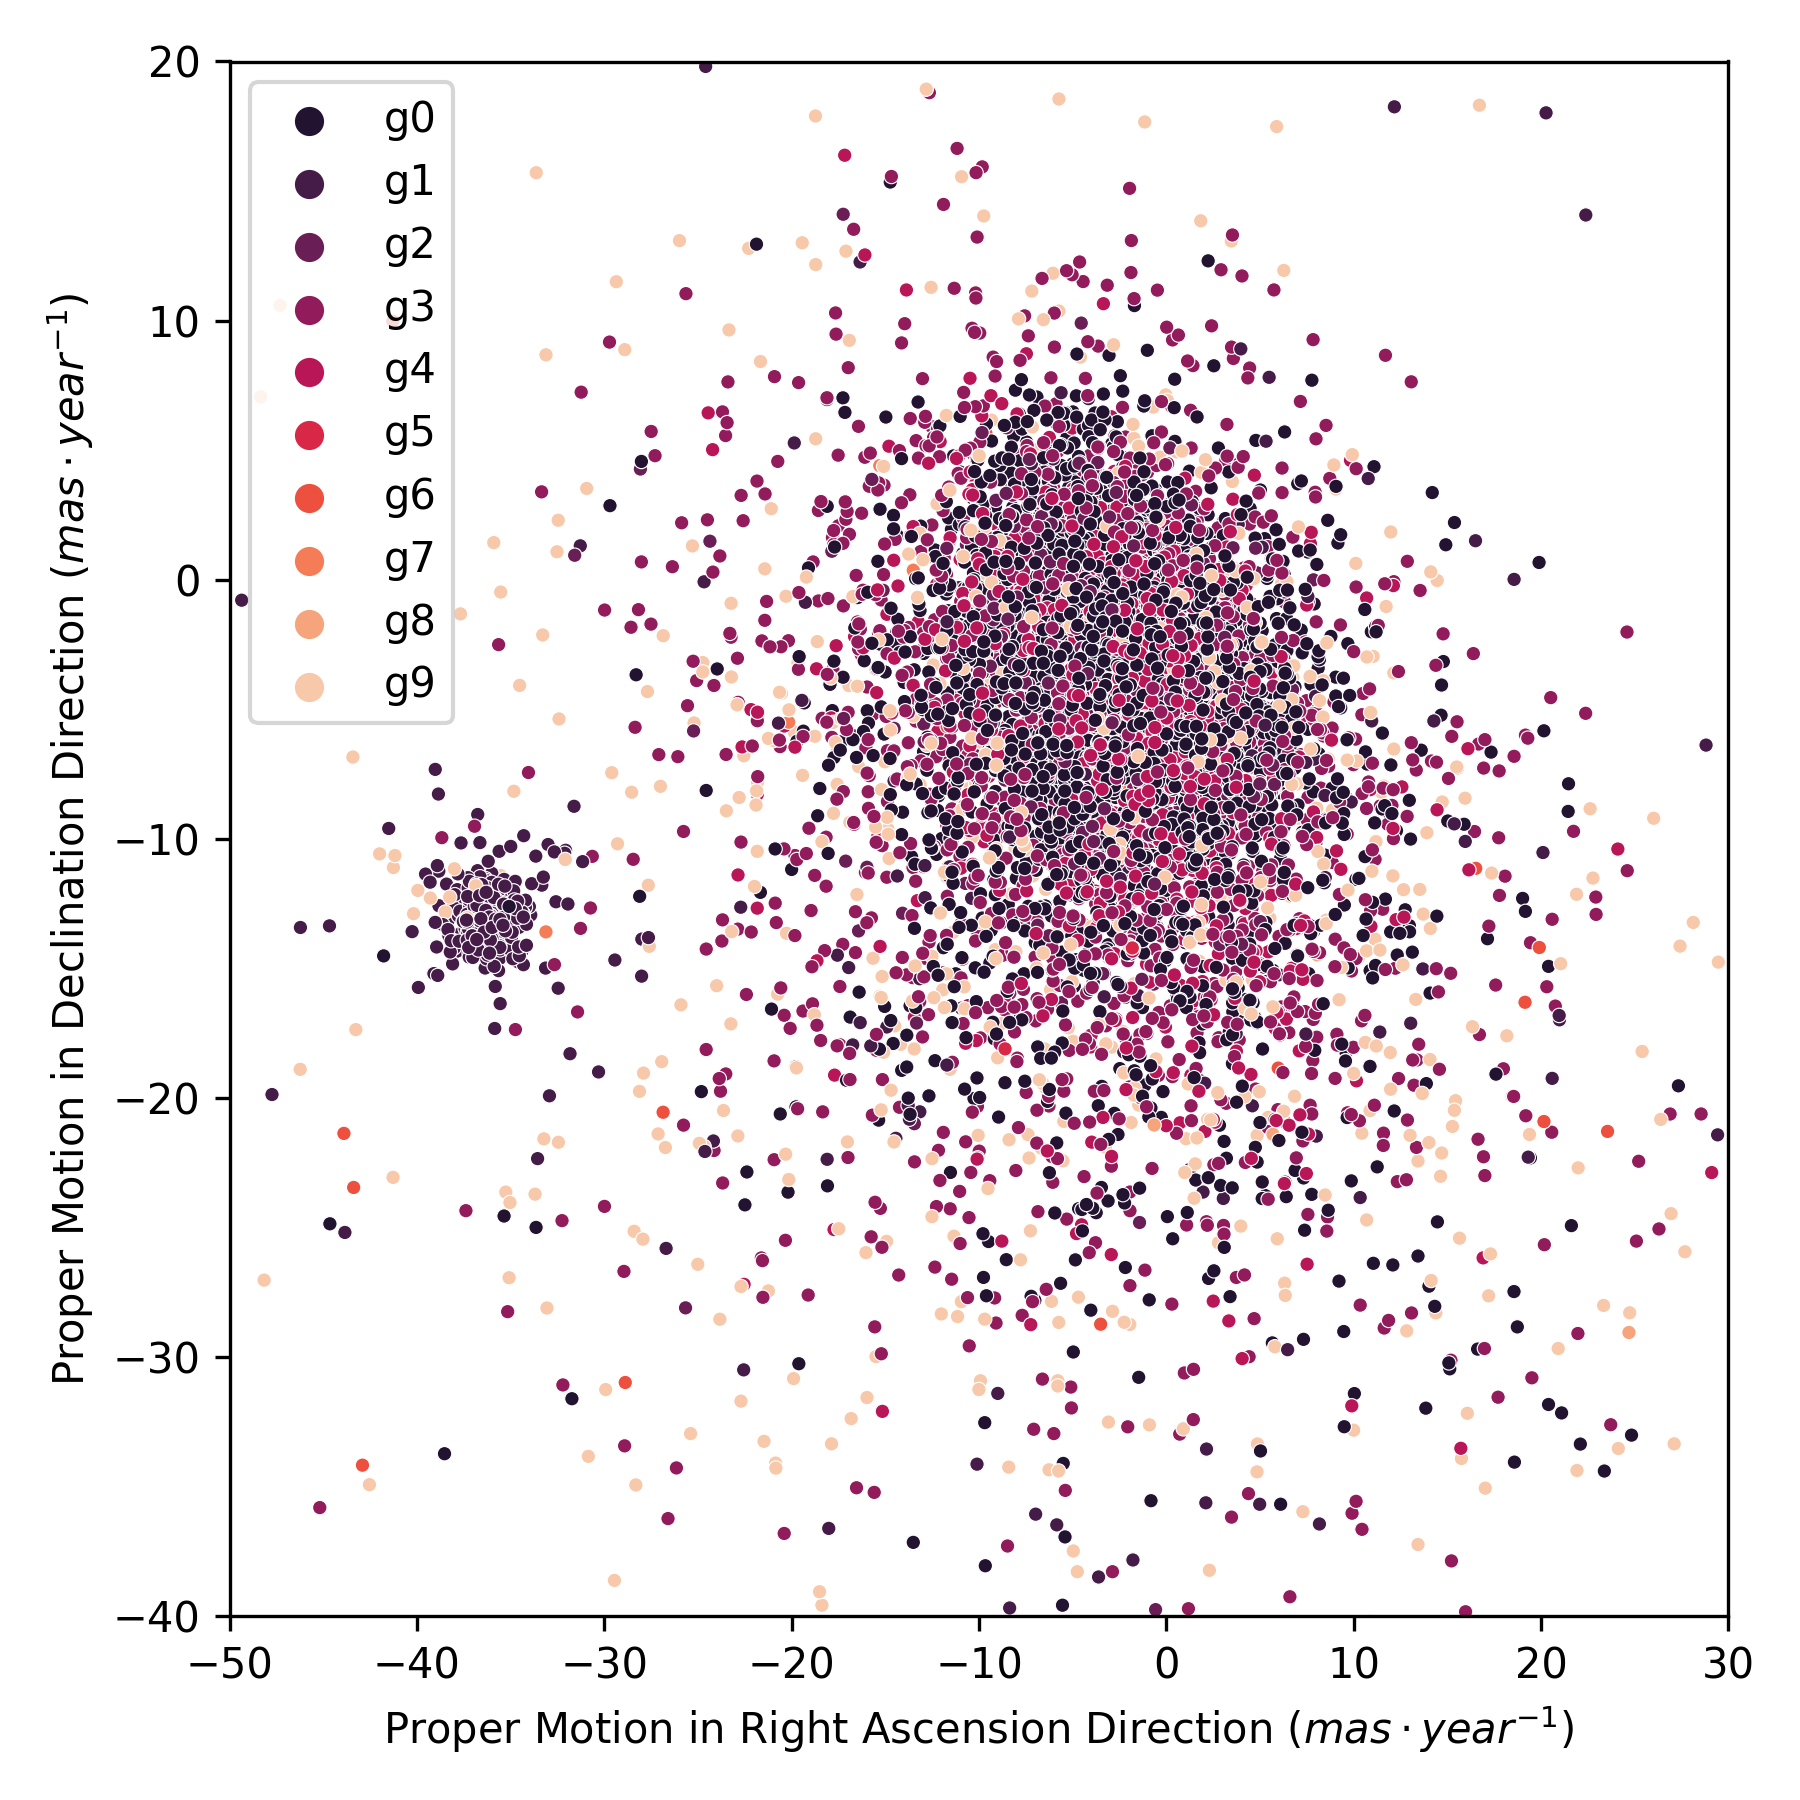
\includegraphics[width=\textwidth]{../figures/ngc_2632/kmeans_pm_ngc_2632.png}
    \end{subfigure}
    \hfill
    \begin{subfigure}[t]{0.30\textwidth}
      \centering
      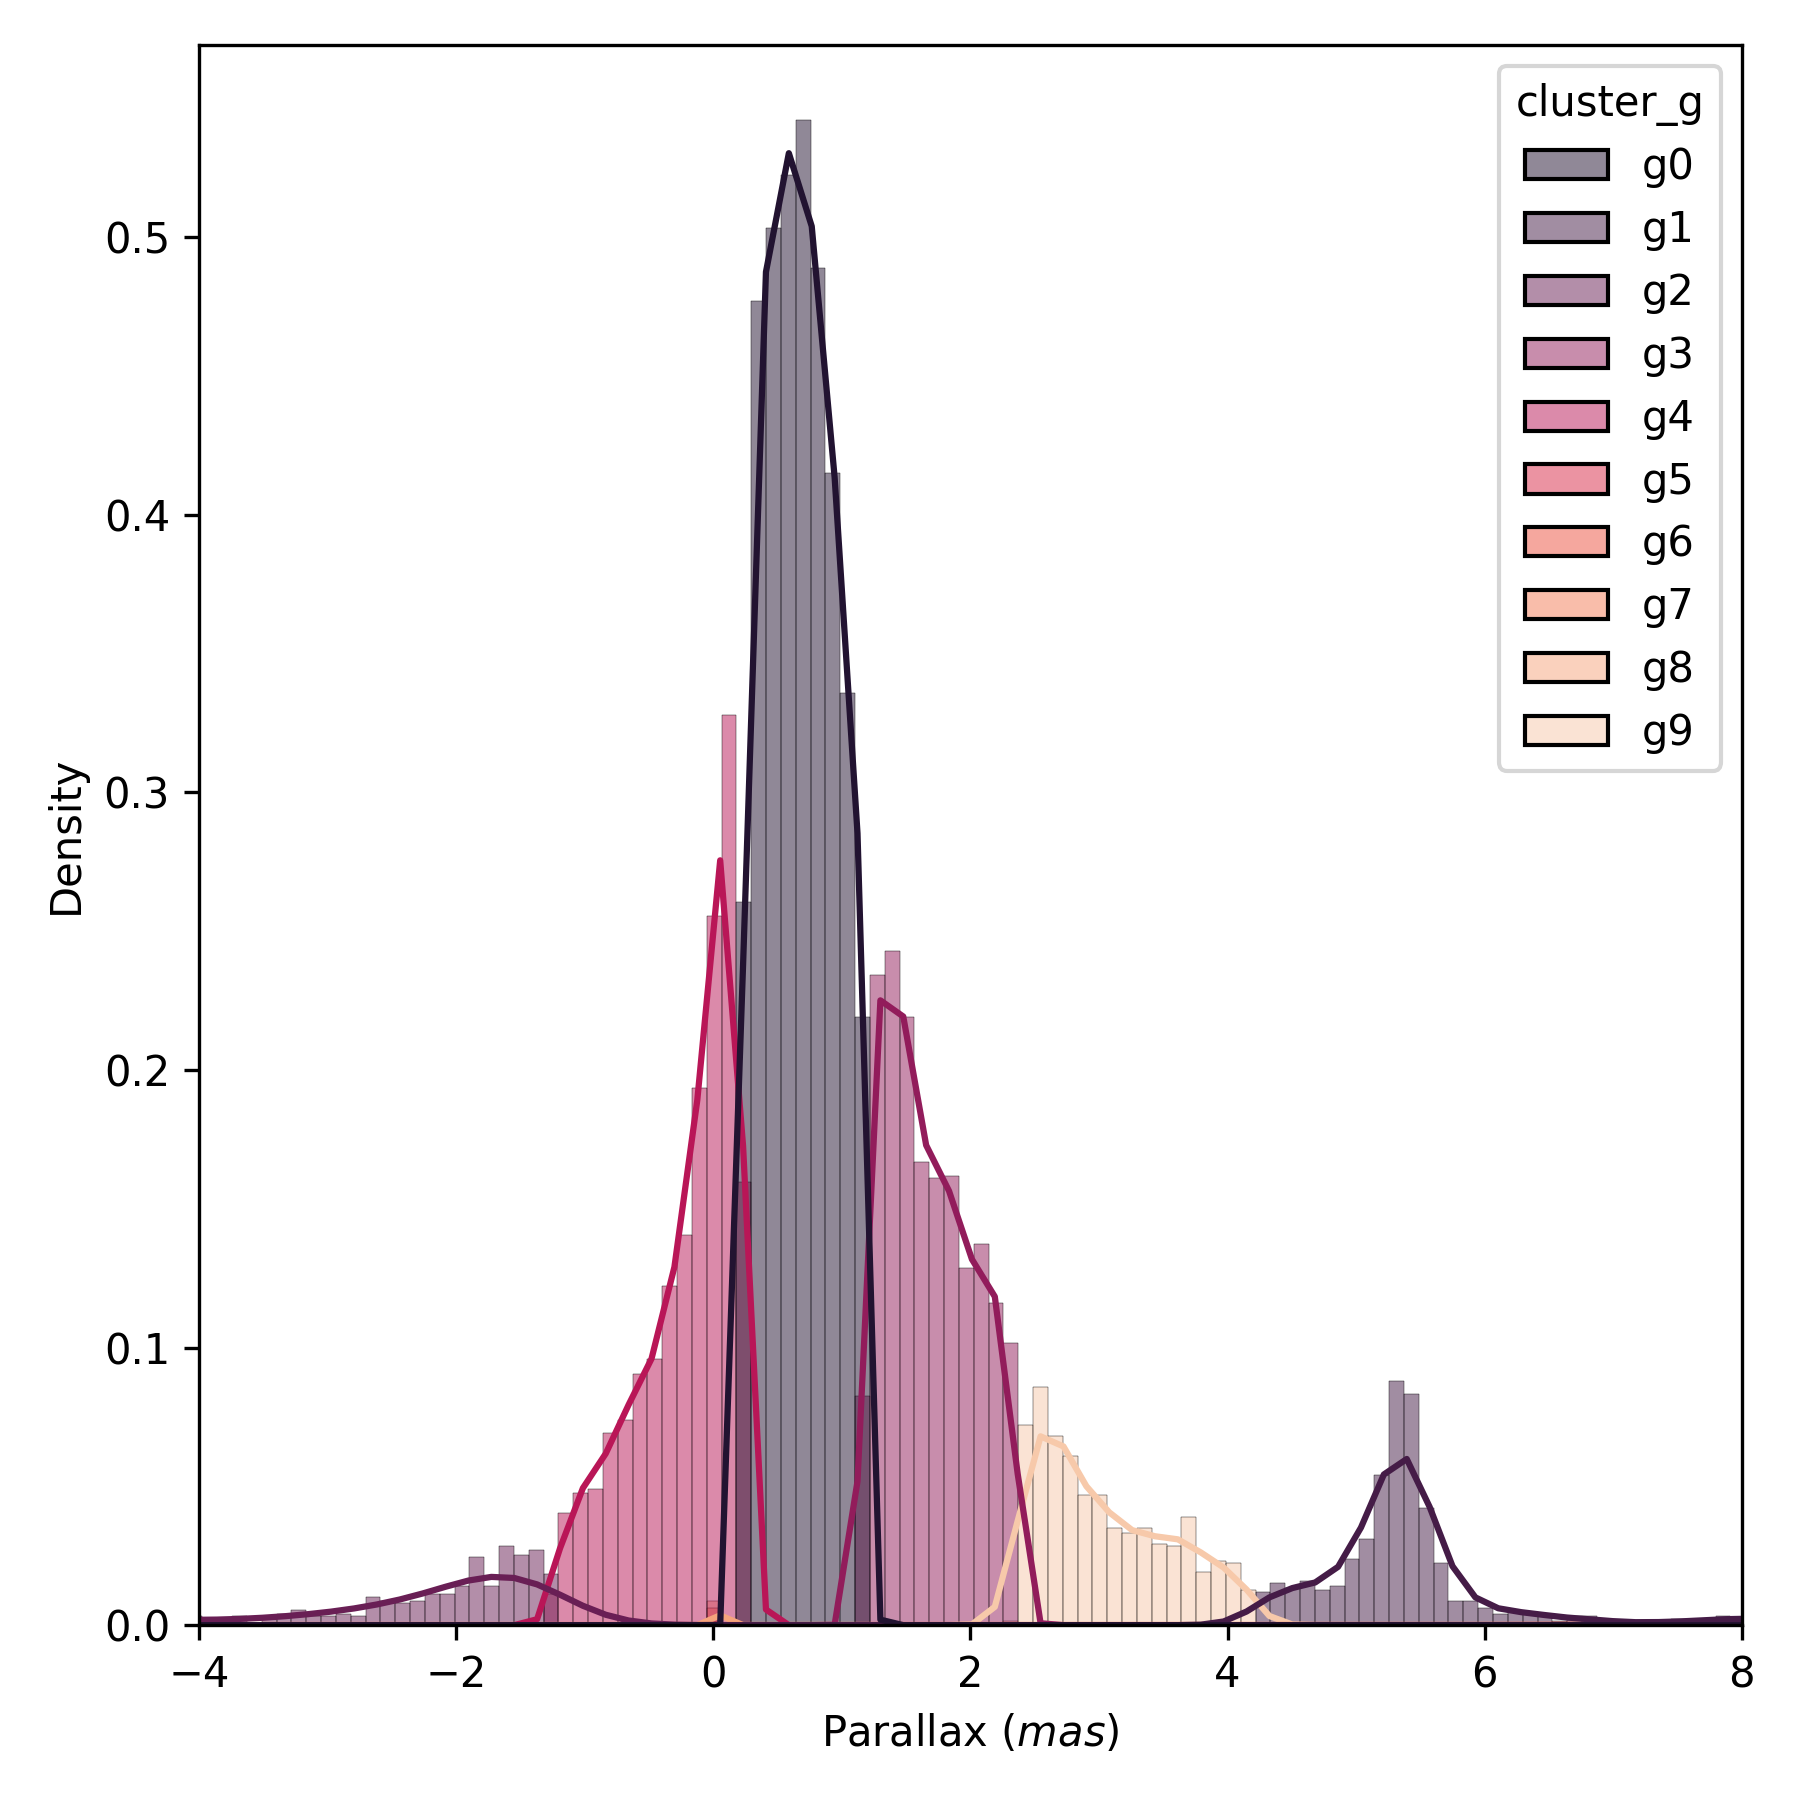
\includegraphics[width=\textwidth]{../figures/ngc_2632/kmeans_parallax_ngc_2632.png}
    \end{subfigure}
    \hfill
    \begin{subfigure}[t]{0.30\textwidth}
      \centering
      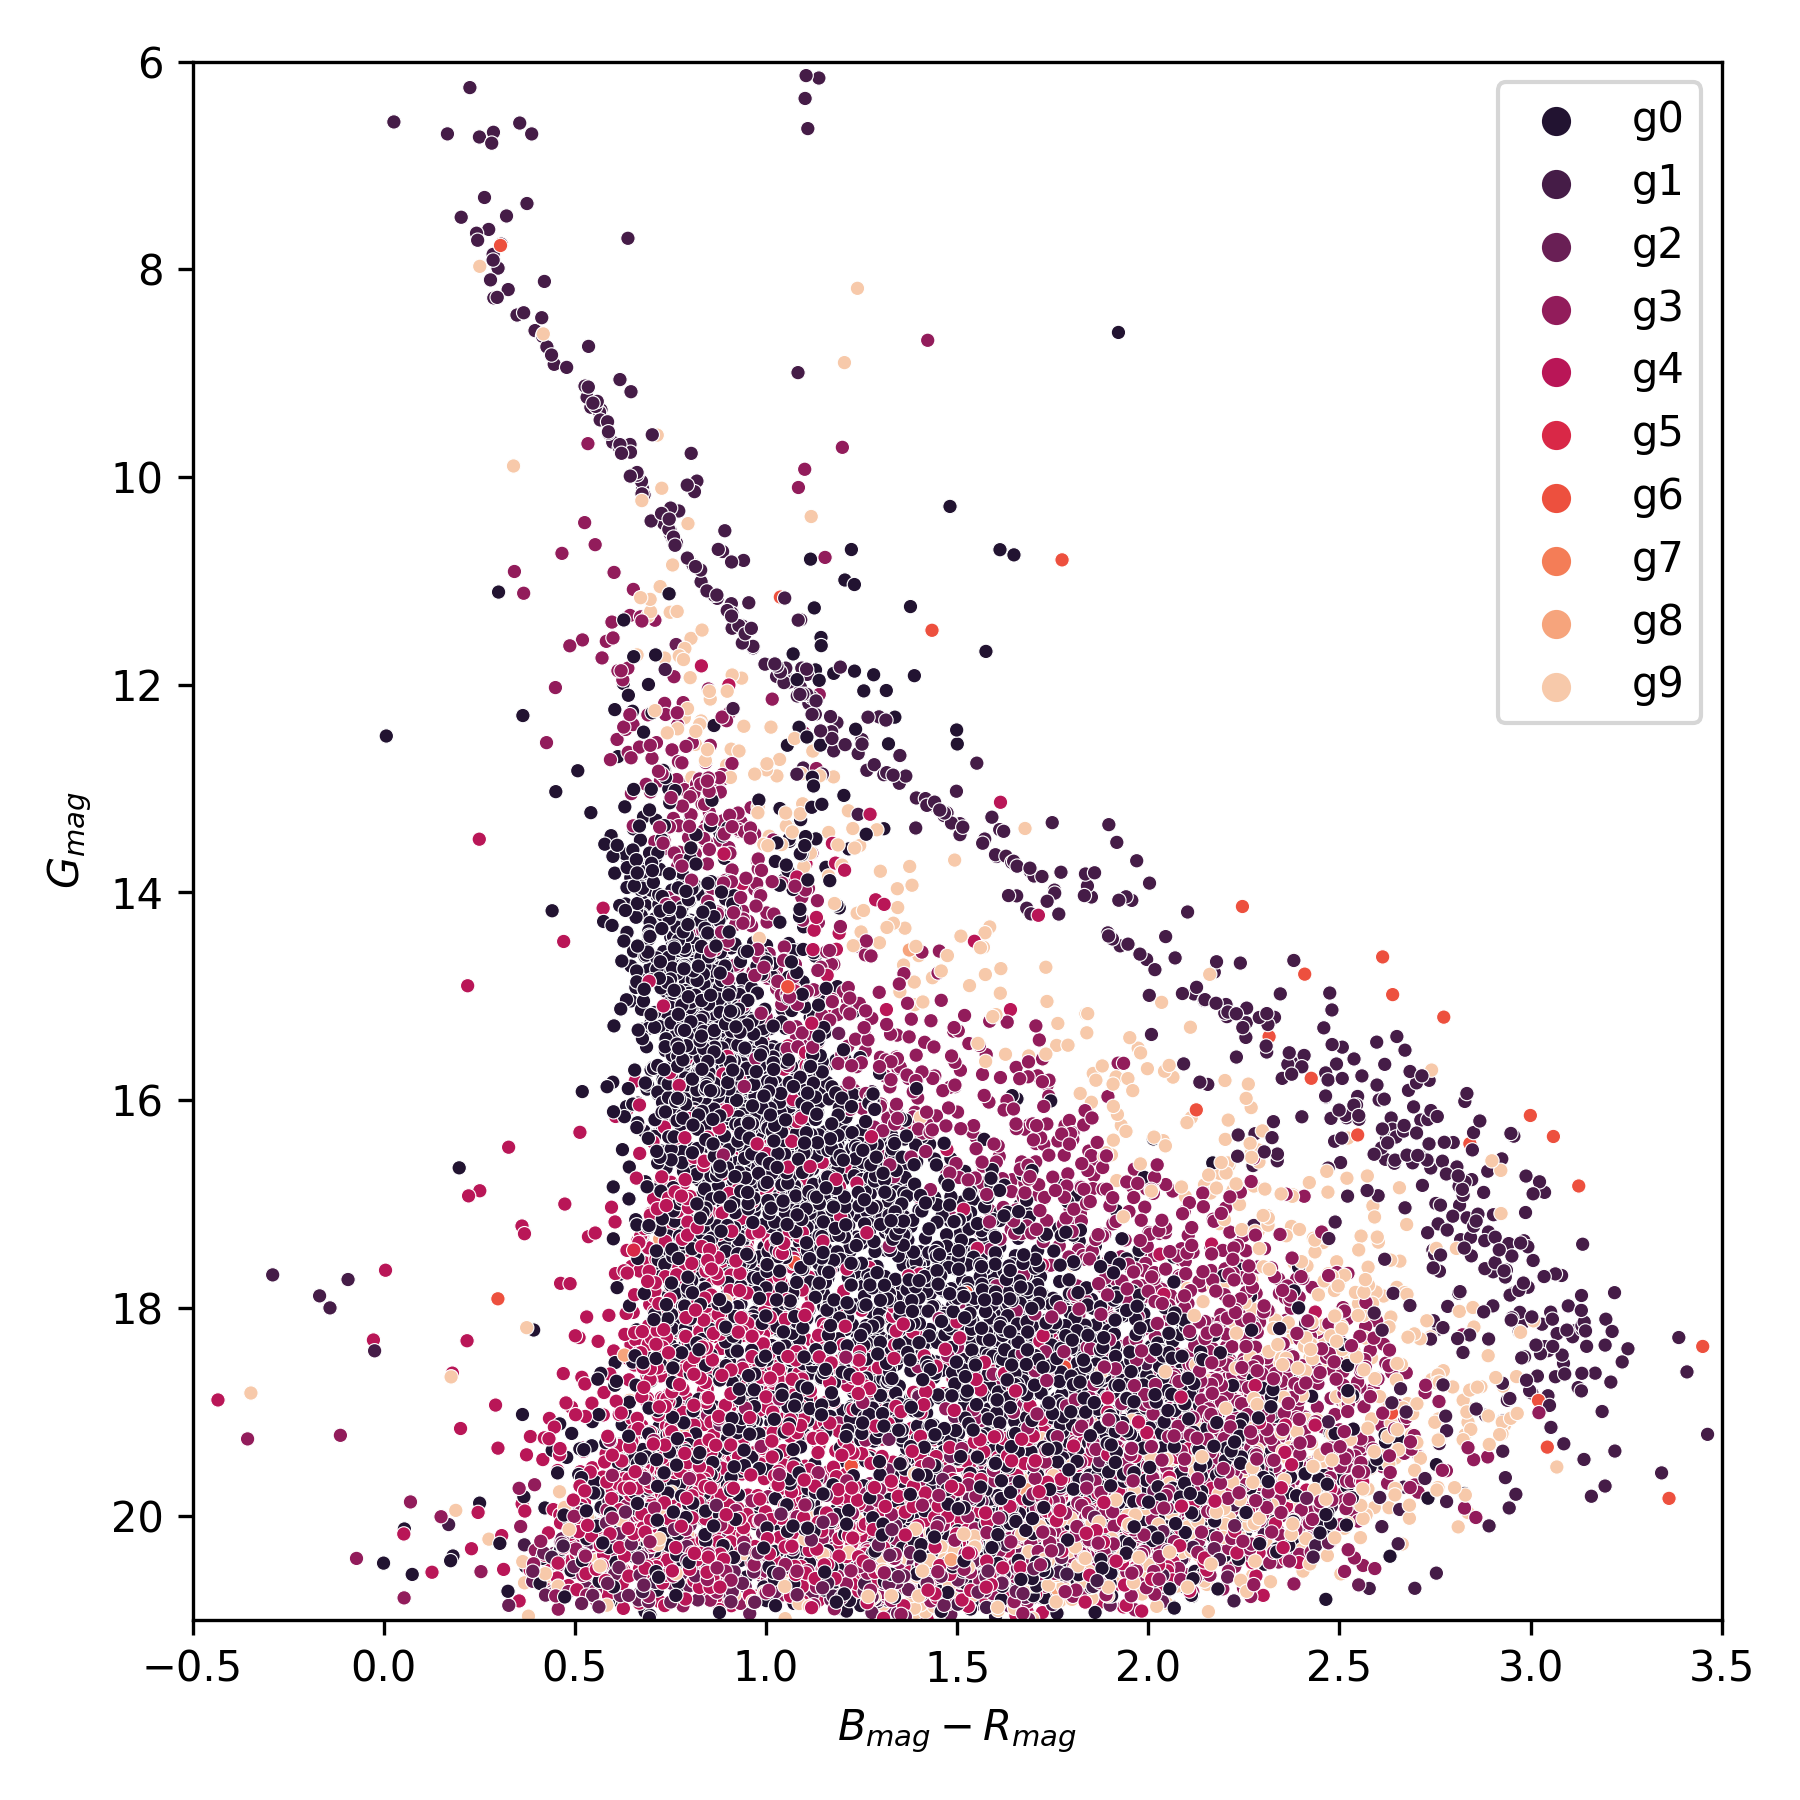
\includegraphics[width=\textwidth]{../figures/ngc_2632/kmeans_hr_diagram_ngc_2632.png}
    \end{subfigure}
  \end{subfigure}
  \caption{NGC 2632 characterization using Clusterix+TOPCAT (top) and K-Means (bottom).
           K-Means identifies NGC 2632 as \emph{g1}.}
  \label{fig:app_result_ngc_2632_clusterix_kmeans}
\end{figure}

Figure \ref{fig:app_result_ngc_2632_dec} shows the groups found using
the DEC model (first row) and the DEC model filtered (second row).
Open cluster NGC 2632 is labeled as group \emph{g1}.

\begin{figure}[htbp]
  \centering
  \begin{subfigure}{\columnwidth}
    \centering
    \begin{subfigure}[t]{0.30\textwidth}
      \centering
      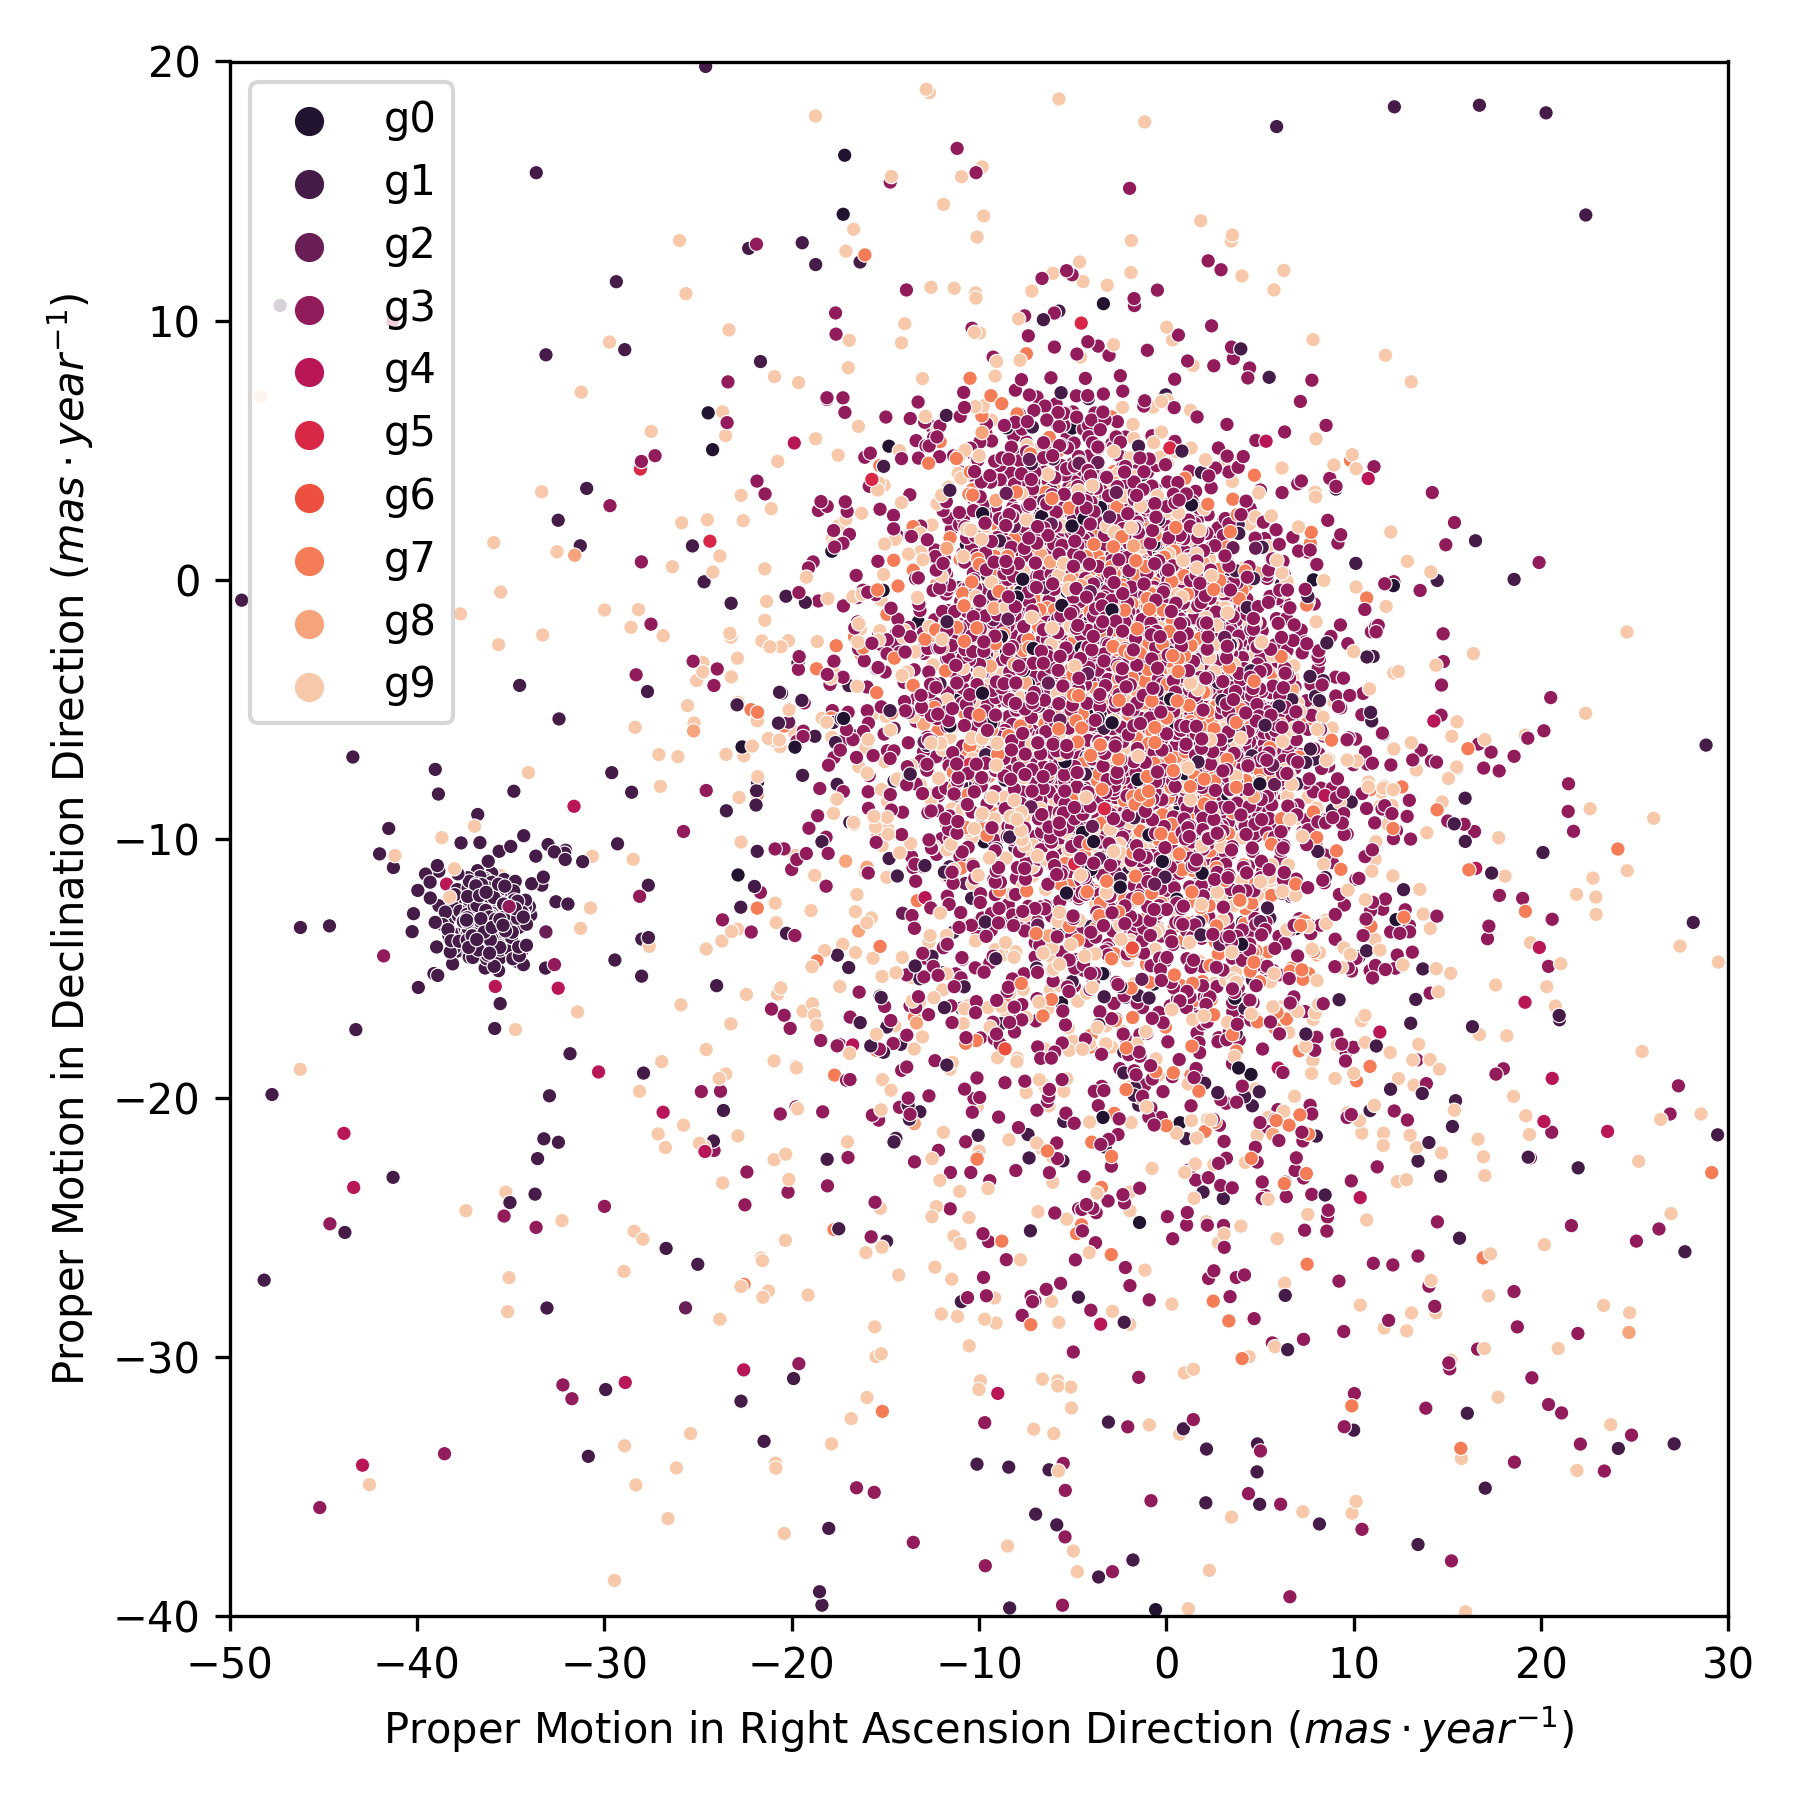
\includegraphics[width=\textwidth]{../figures/ngc_2632/dec_pm_ngc_2632.png}
    \end{subfigure}
    \hfill
    \begin{subfigure}[t]{0.30\textwidth}
      \centering
      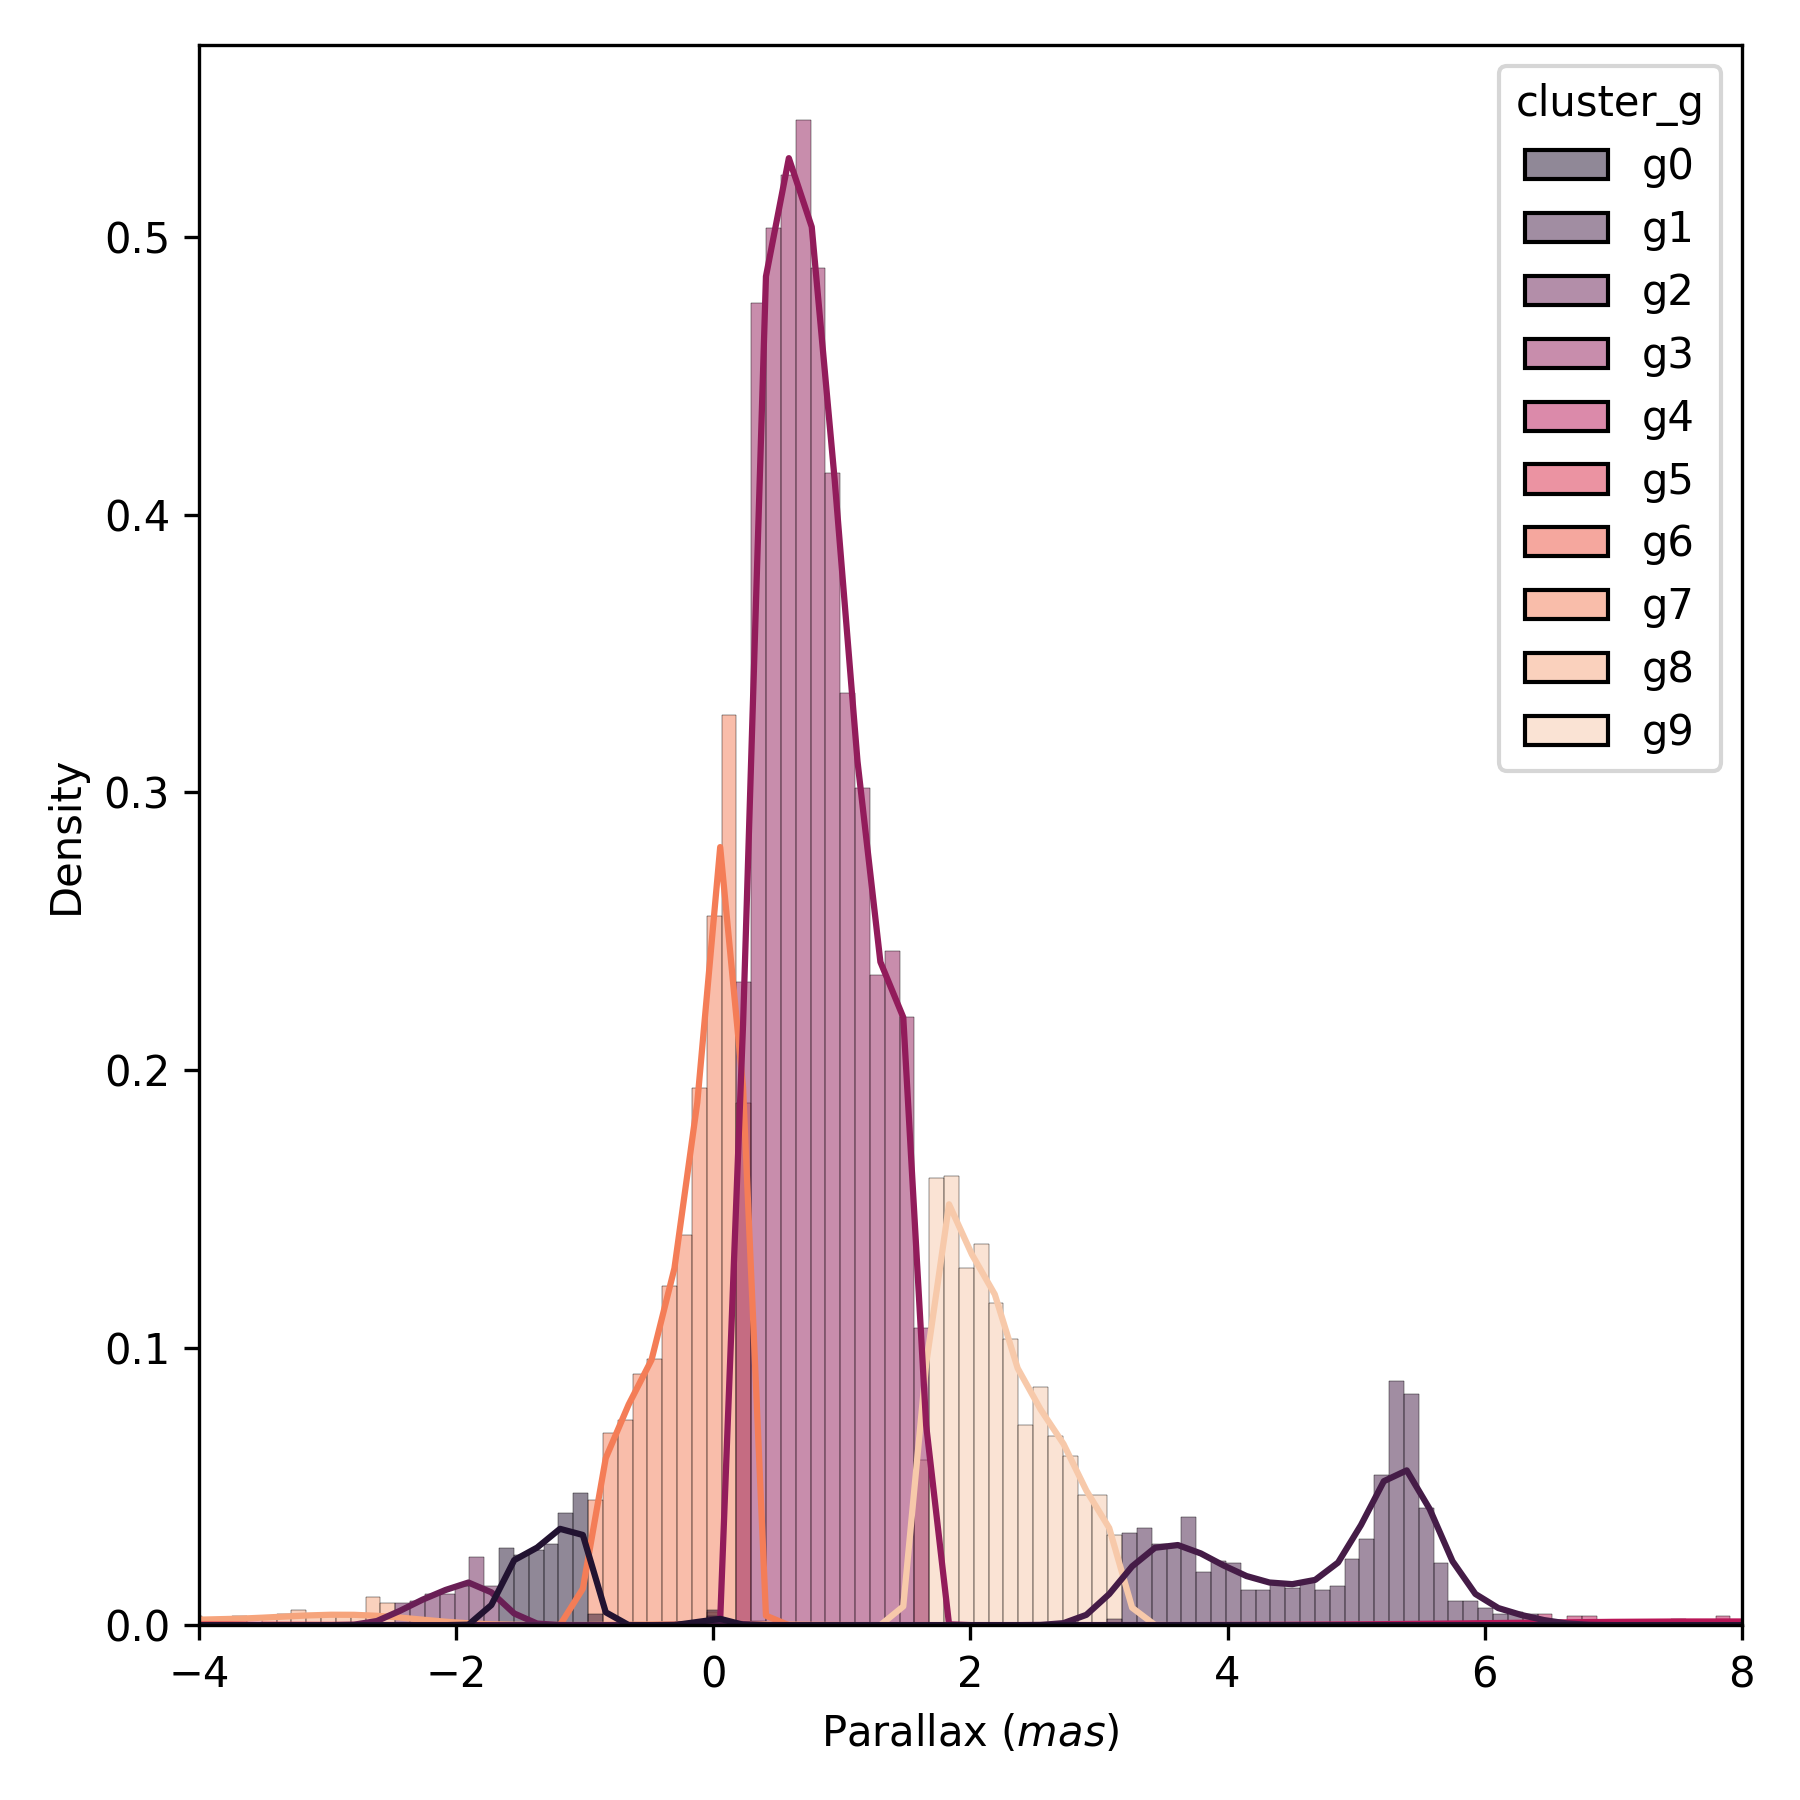
\includegraphics[width=\textwidth]{../figures/ngc_2632/dec_parallax_ngc_2632.png}
    \end{subfigure}
    \hfill
    \begin{subfigure}[t]{0.30\textwidth}
      \centering
      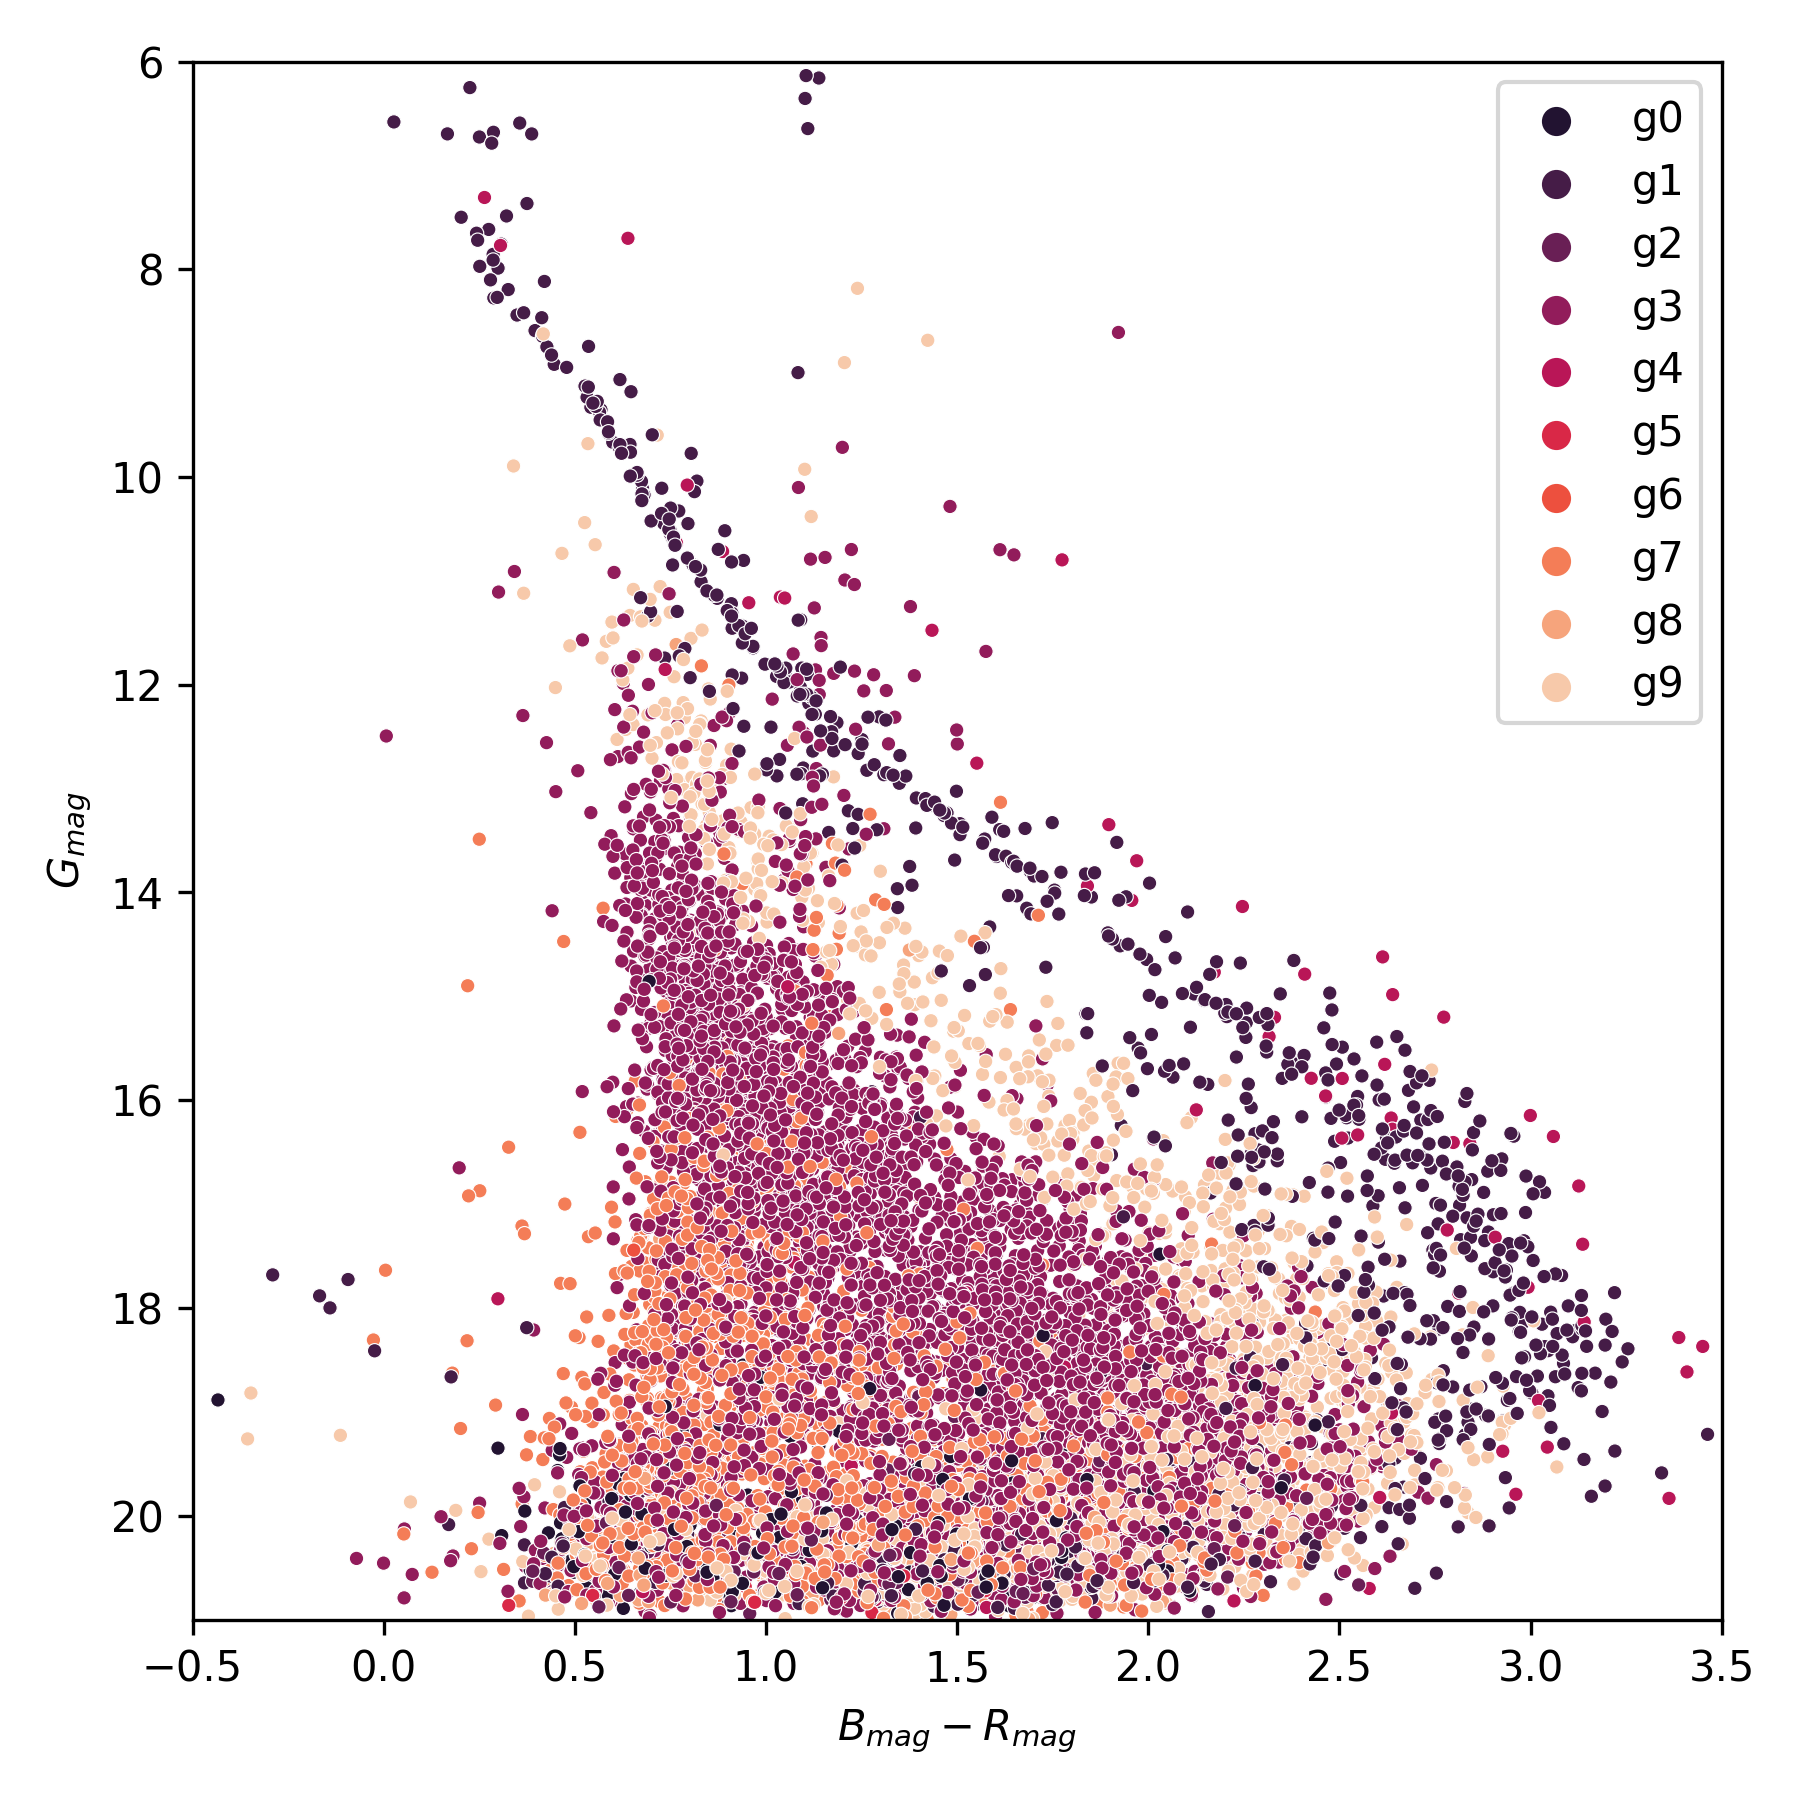
\includegraphics[width=\textwidth]{../figures/ngc_2632/dec_hr_diagram_ngc_2632.png}
    \end{subfigure}
  \end{subfigure}
  \centering
  \begin{subfigure}{\columnwidth}
    \centering
    \begin{subfigure}[t]{0.30\textwidth}
      \centering
      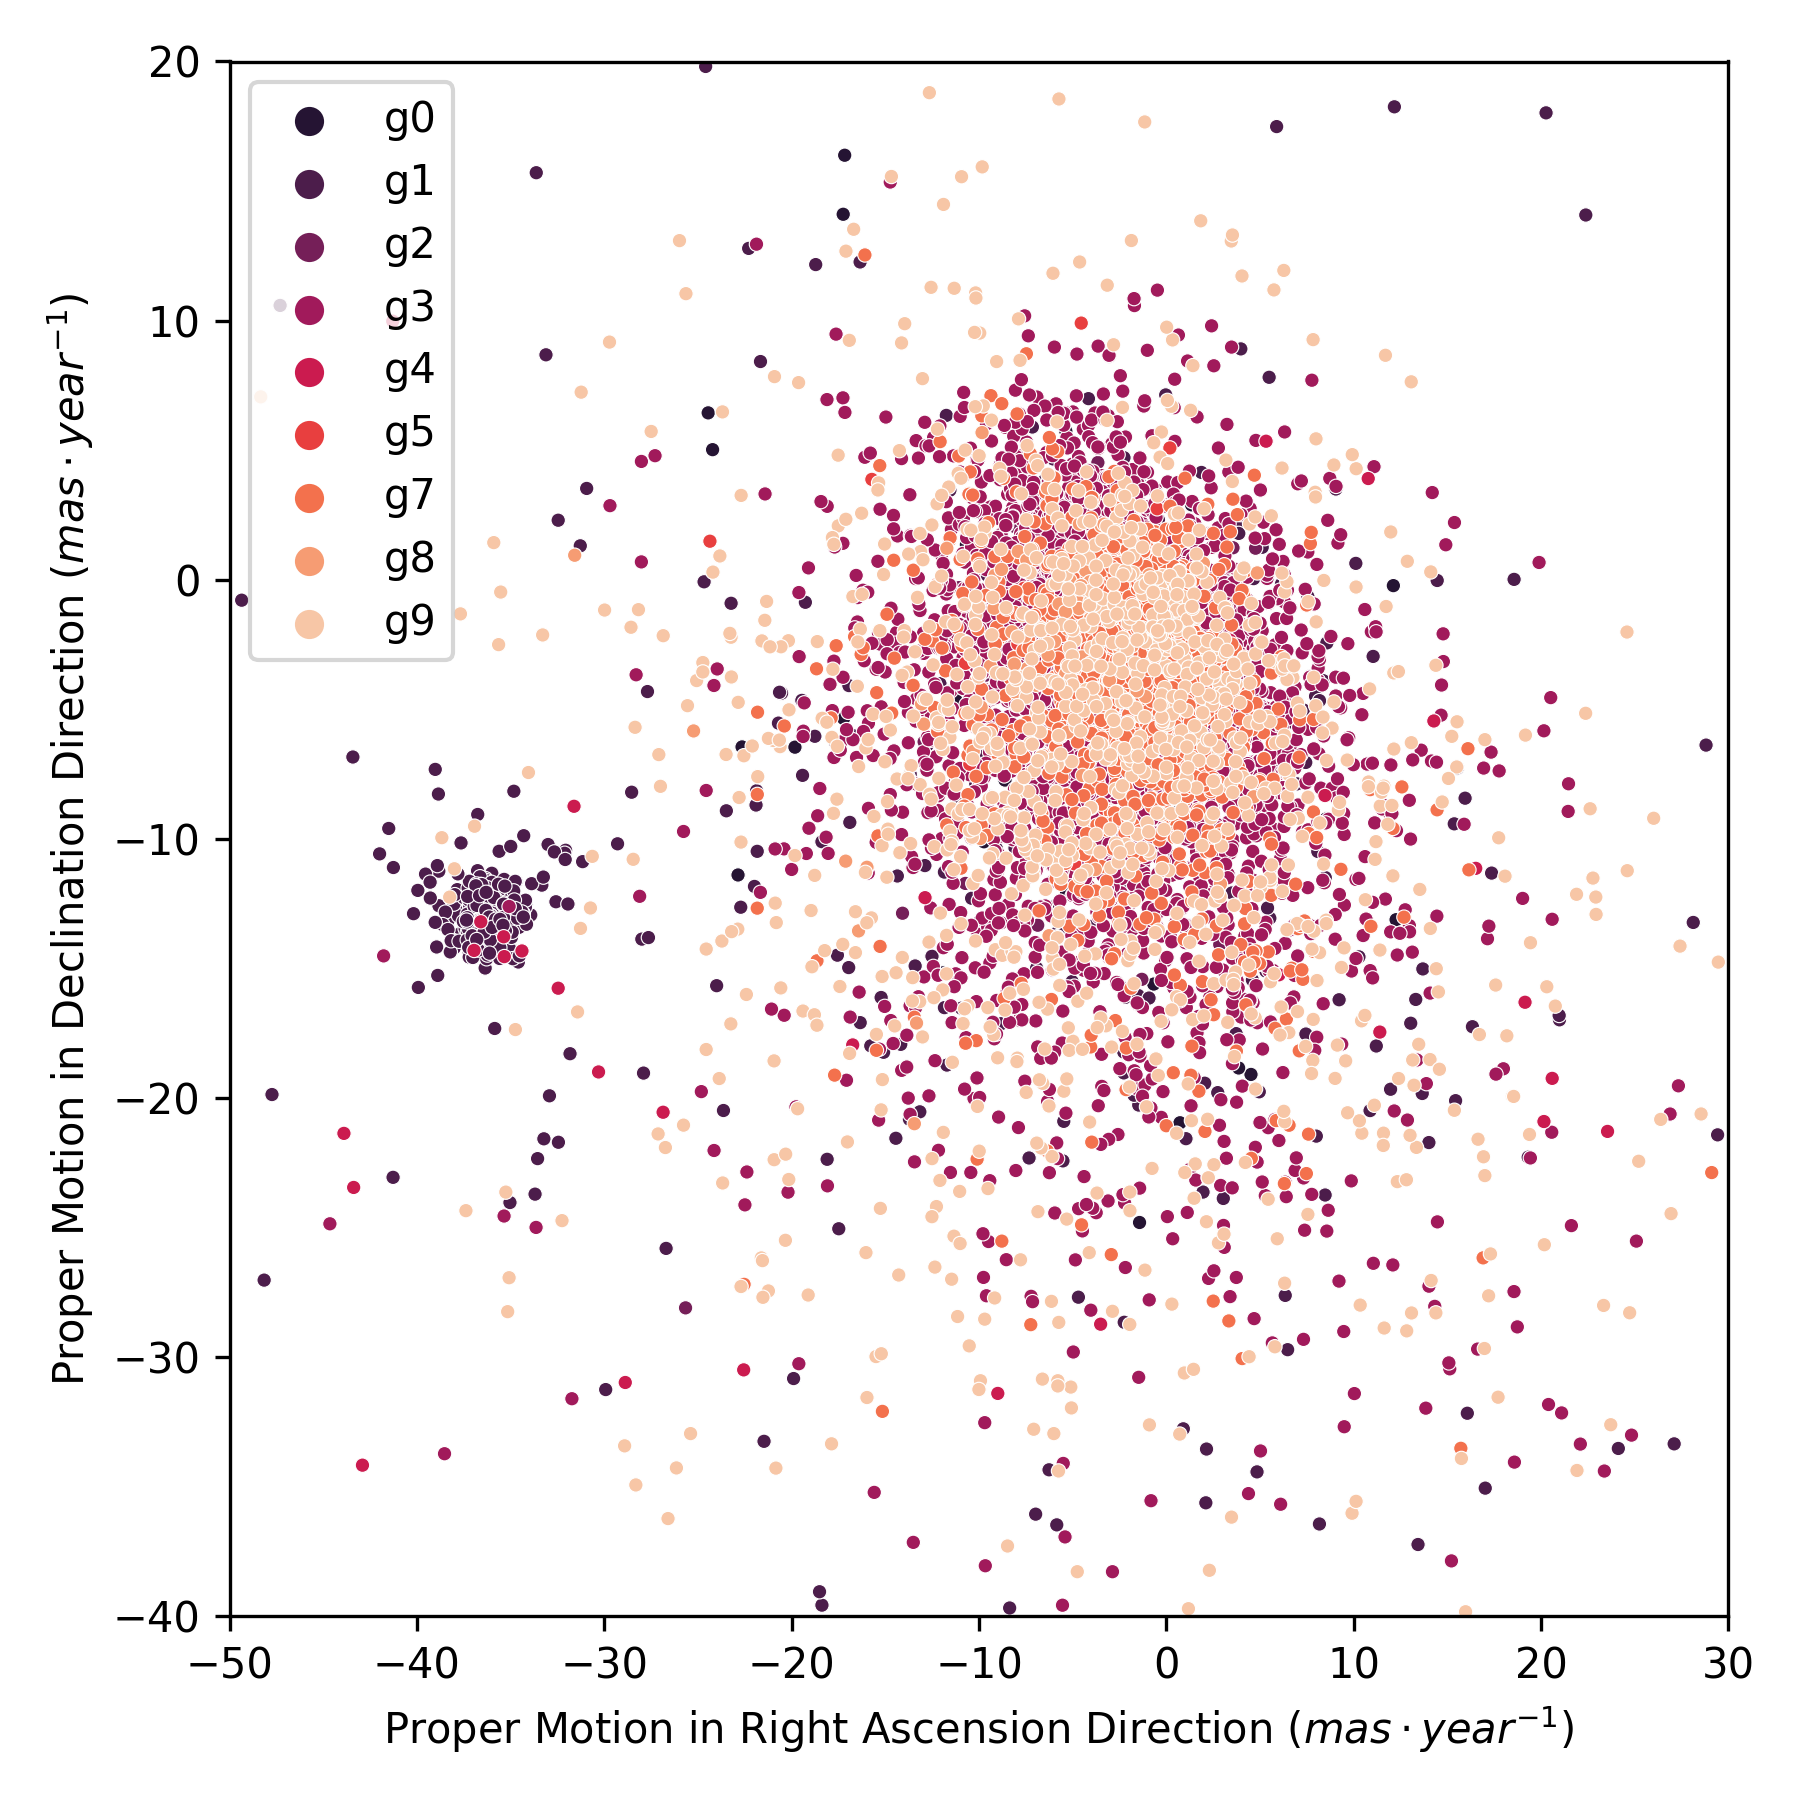
\includegraphics[width=\textwidth]{../figures/ngc_2632/dec_pm_filtered_ngc_2632.png}
    \end{subfigure}
    \hfill
    \begin{subfigure}[t]{0.30\textwidth}
      \centering
      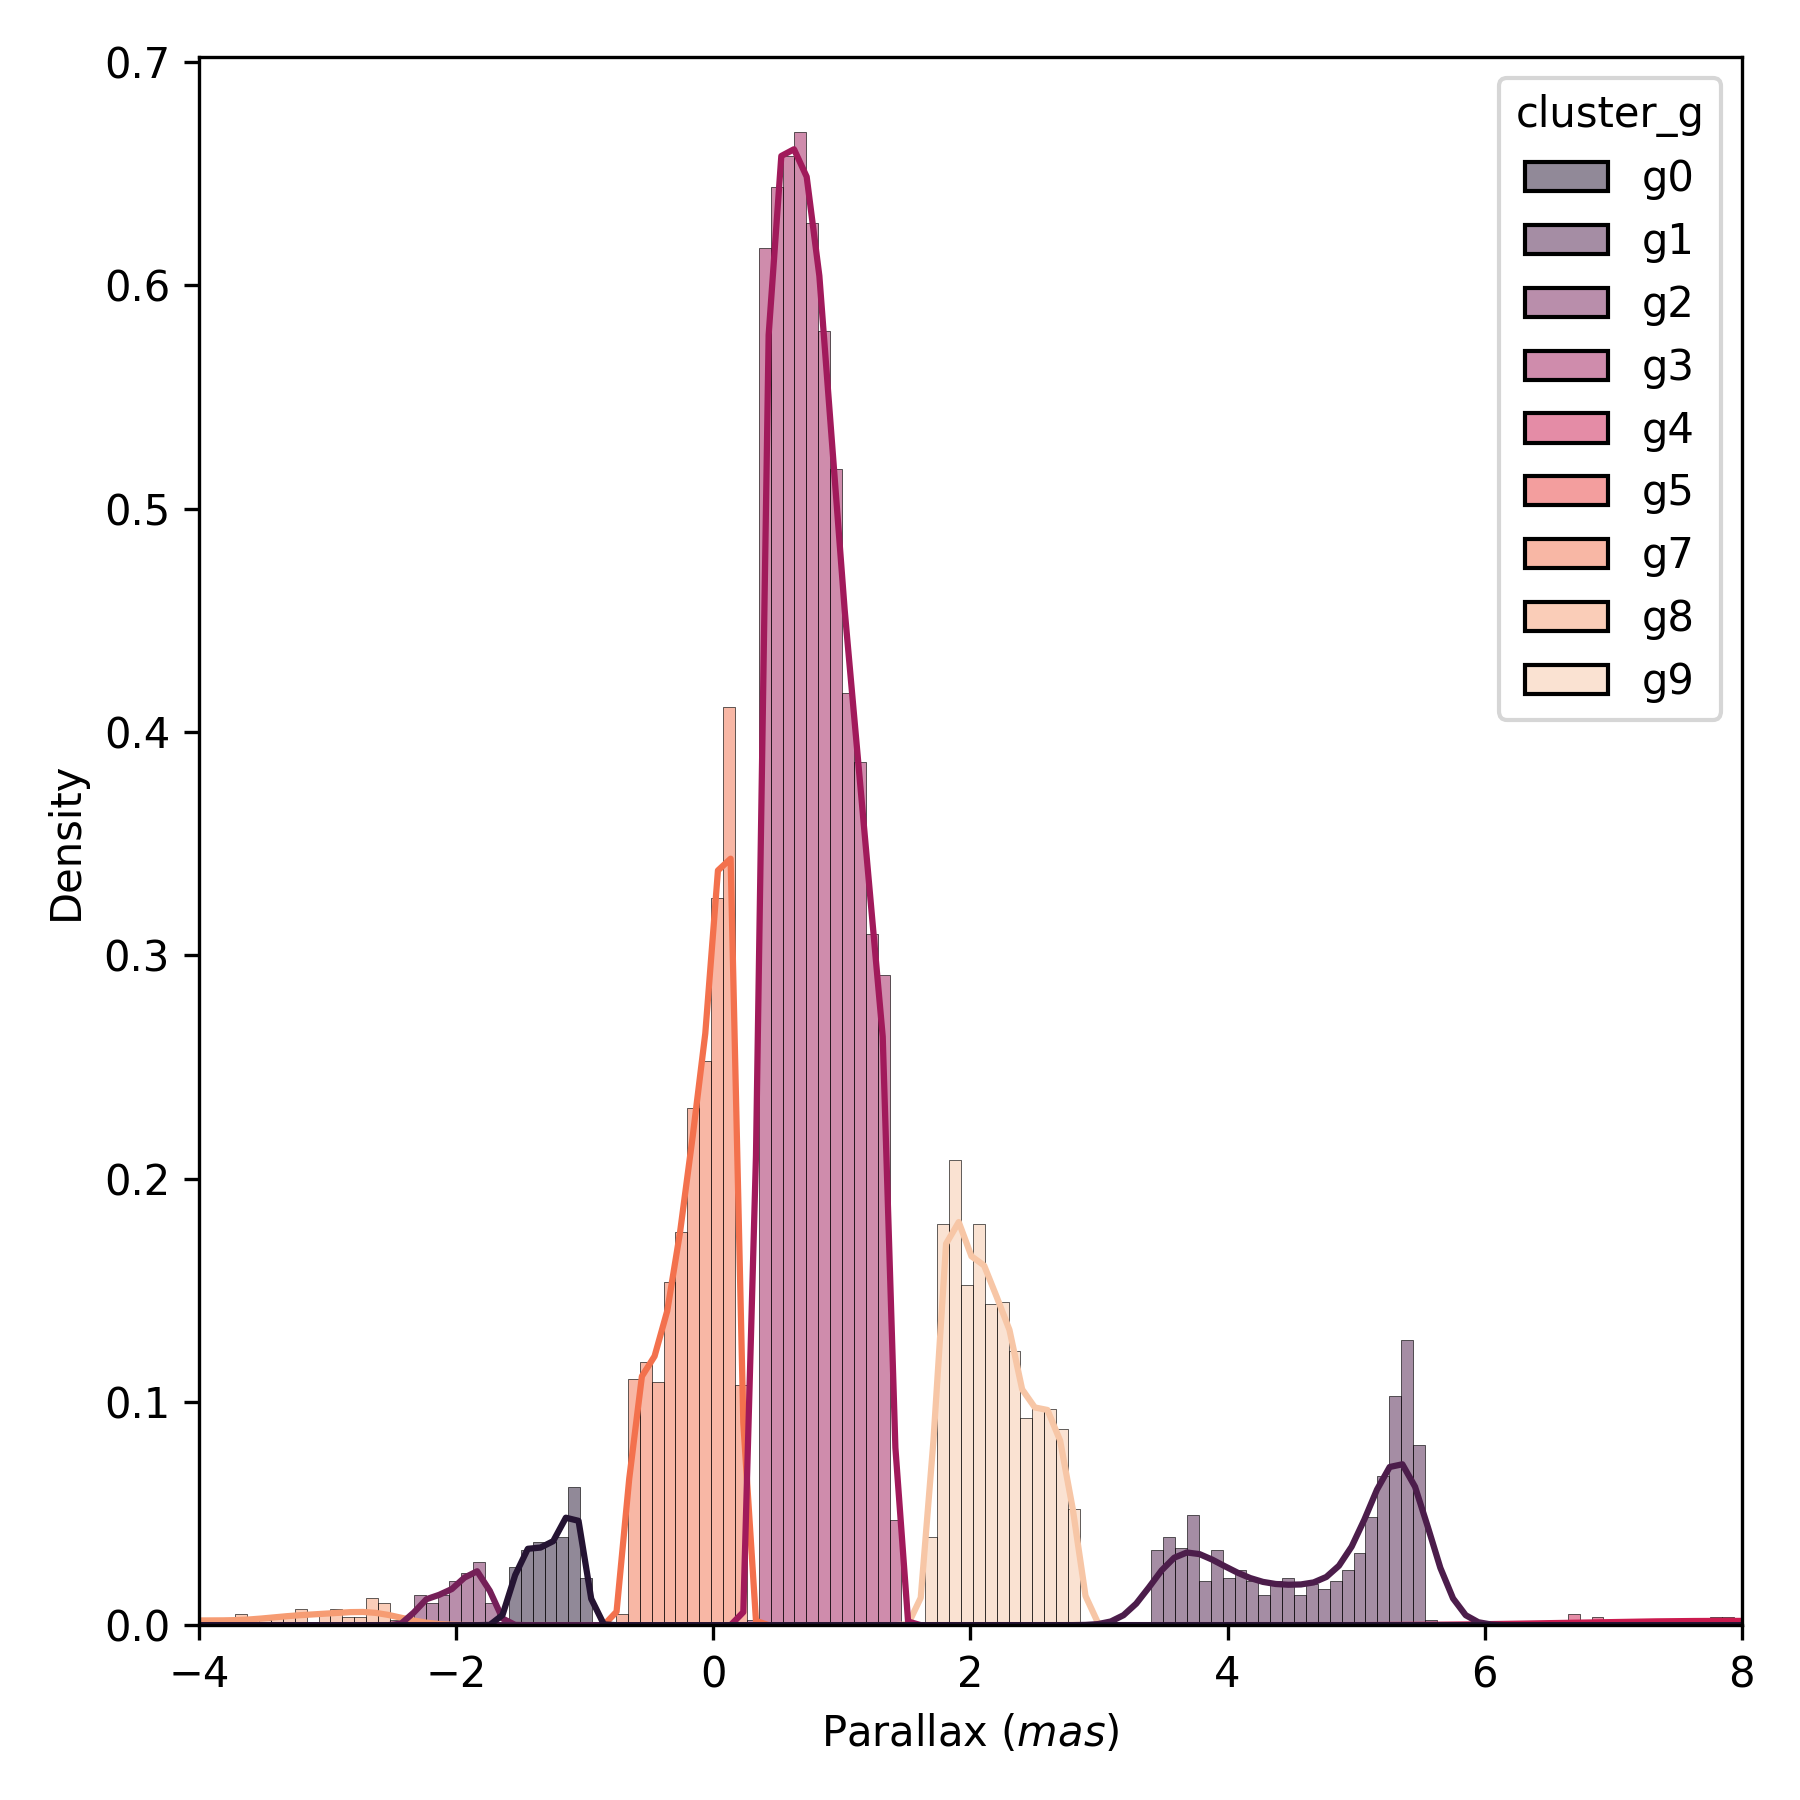
\includegraphics[width=\textwidth]{../figures/ngc_2632/dec_parallax_filtered_ngc_2632.png}
    \end{subfigure}
    \hfill
    \begin{subfigure}[t]{0.30\textwidth}
      \centering
      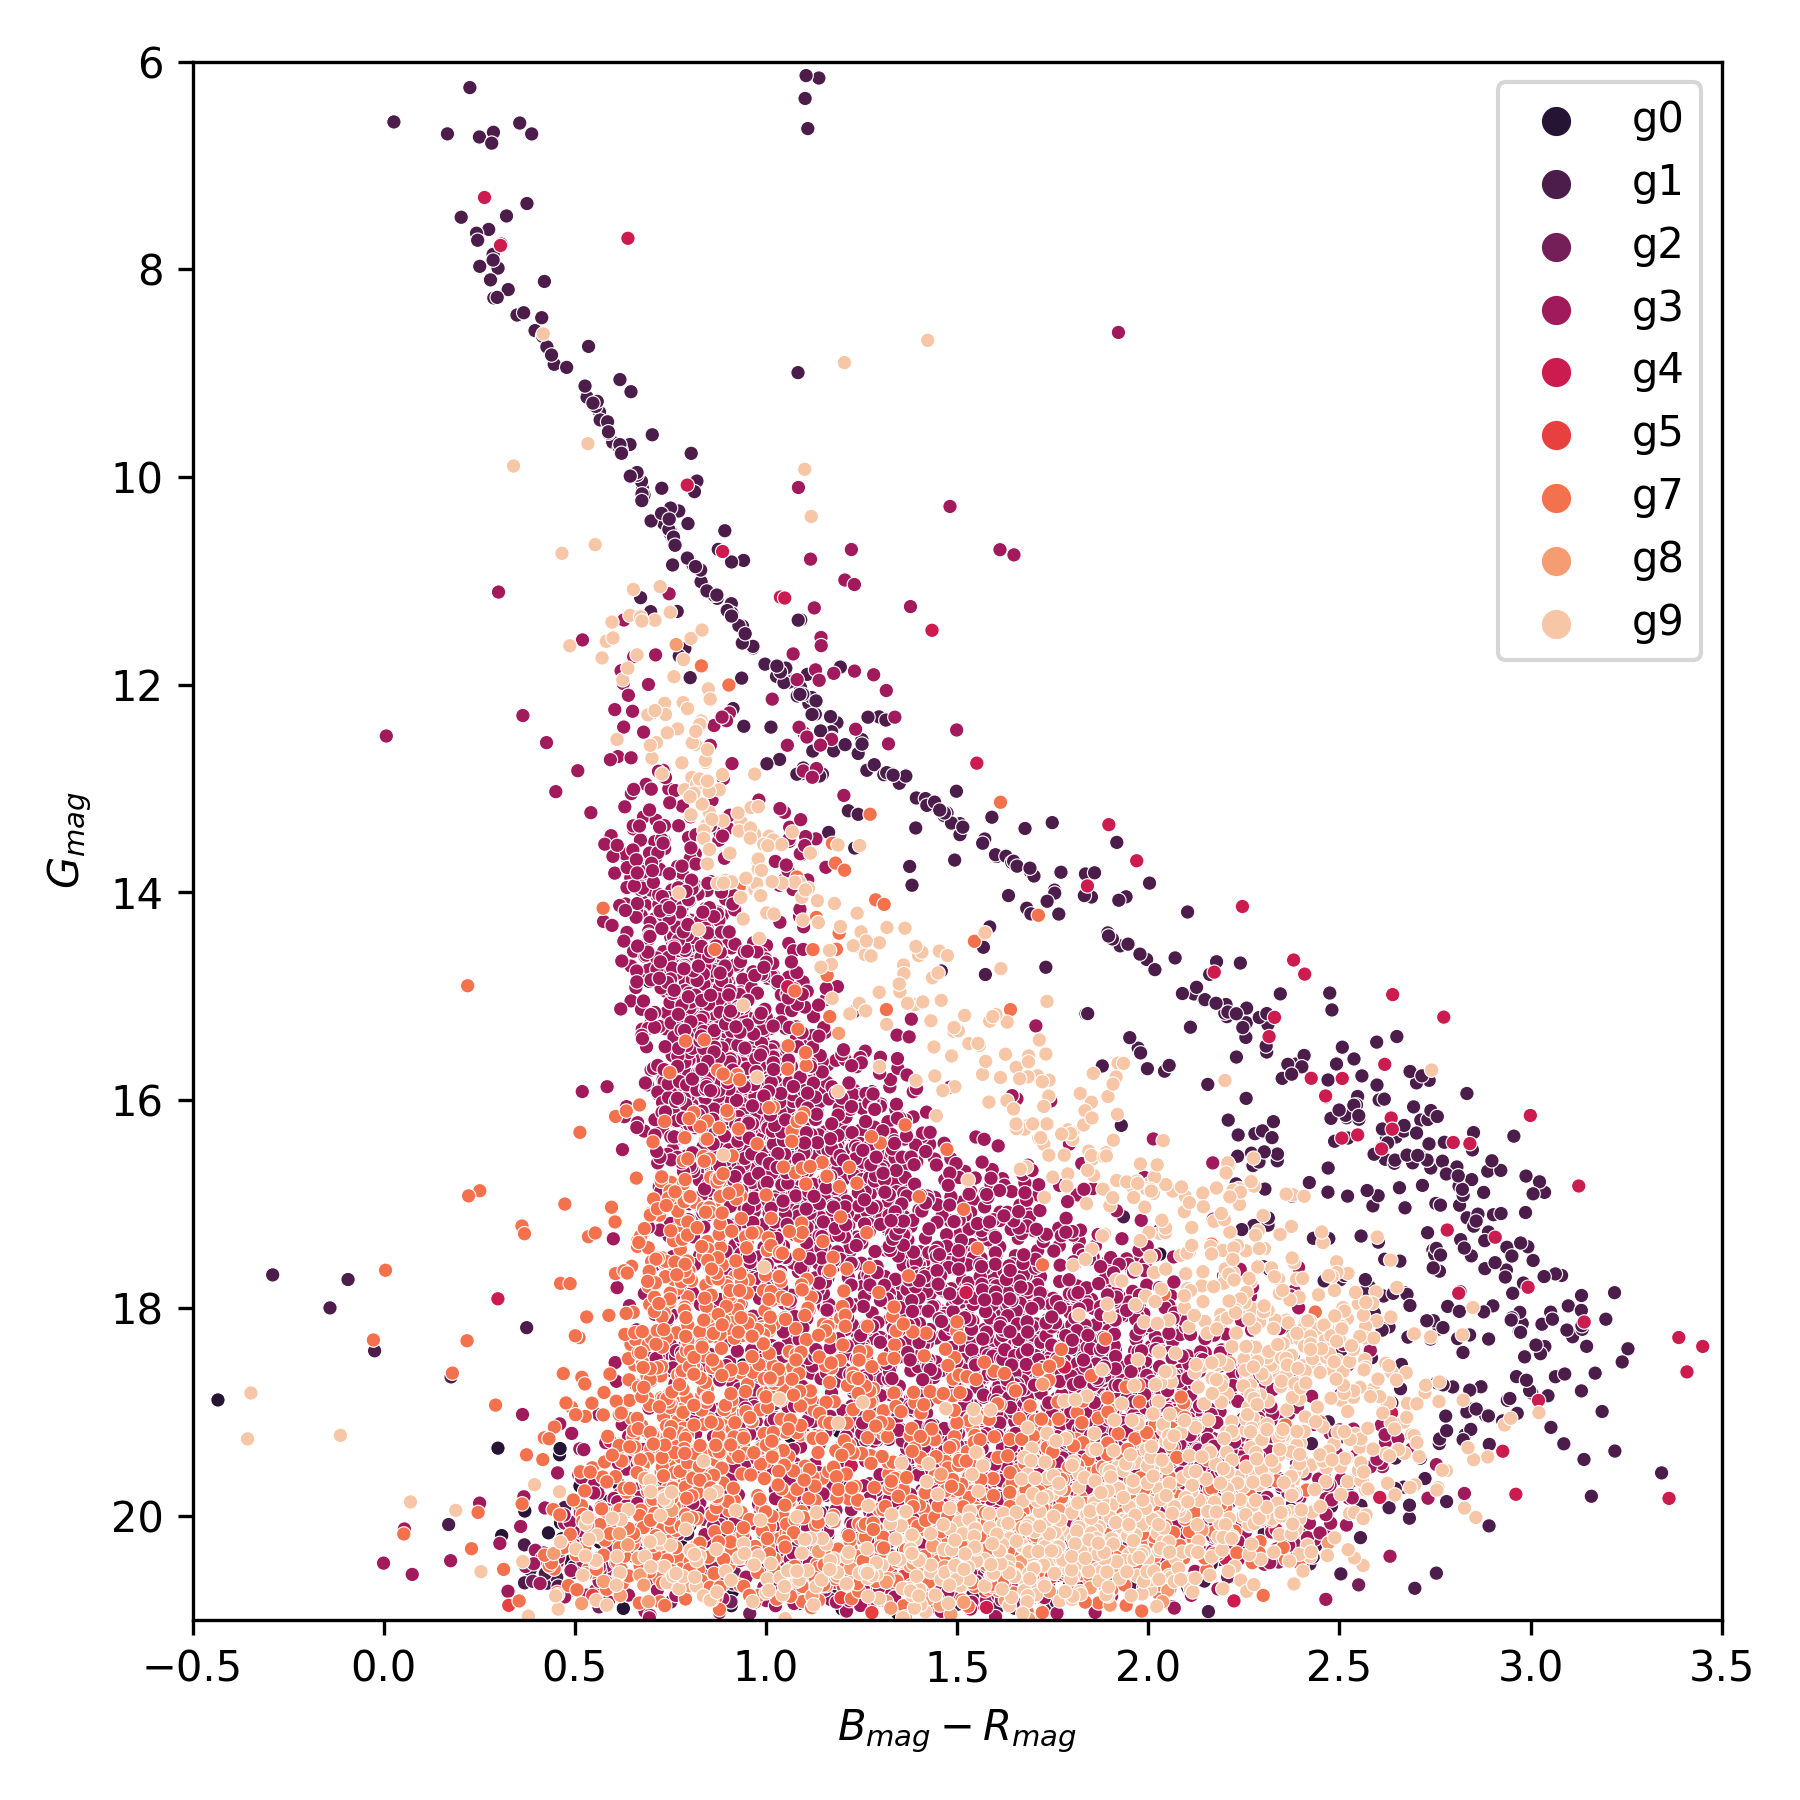
\includegraphics[width=\textwidth]{../figures/ngc_2632/dec_hr_diagram_filtered_ngc_2632.png}
    \end{subfigure}
  \end{subfigure}
  \caption{NGC 2632 characterization using DEC model (top) and DEC (filtered) (bottom).
           NGC 2632 is identified as \emph{g1}.}
  \label{fig:app_result_ngc_2632_dec}
\end{figure}

\begin{table}[htbp]
  \begin{center}
    \resizebox{\columnwidth}{!}{
      \begin{tabular}{l|c|c|c|c}
        \textbf{Method} & \emph{$\mu_{\alpha}$ $(mas/yr^{-1})$} & \emph{$\mu_{\delta}$ $(mas/yr^{-1})$} & \emph{$\varpi$ $(mas)$} & \emph{\# stars} \\
        \hline
        \textbf{Simbad} & -36.047 $\pm$ 0.110 & -12.917 $\pm$ 0.066 & 5.371 $\pm$ 0.003 & - \\
        Clusterix & -36.154 $\pm$ 1.001 & -12.909 $\pm$ 0.806 & 5.327 $\pm$ 0.187 & 371 \\
        K-Means & -26.352 $\pm$ 0.82 & -15.828 $\pm$ 0.76 & 5.394 $\pm$ 0.03 & 629 \\
        DEC & -20.012 $\pm$ 0.69 & -14.742 $\pm$ 0.58 & 4.686 $\pm$ 0.03 & 894 \\
        \textbf{DEC (filt.)} & -21.571 $\pm$ 0.74 & -14.234 $\pm$ 0.61 & 4.719 $\pm$ 0.03 & 714 \\
      \end{tabular}
    }
    \caption{NGC 2632 results.}
    \label{tab:app_results_ngc_2632}
  \end{center}
\end{table}

Table \ref{tab:app_results_ngc_2632} shows a results summary for NGC 2632 analysis.
While Table \ref{tab:app_hyperparameters_ngc_2632} shows the hyperparameters
used for characterizing NGC 2632 with our model.

\begin{table}[htbp]
  \begin{center}
    \begin{tabular}{l|c}
      \textbf{Hyperparameter} & \textbf{Value} \\
      \hline
      Number of Clusters & 10 \\
      Clustering Layer & $\left[ 50, 50, 40 \right]$ \\
      Kernel Initializer Seed & 10 \\
      Quantil Threshold & 0.1 \\
    \end{tabular}
    \caption{NGC 2632 DEC hyperparameters.}
    \label{tab:app_hyperparameters_ngc_2632}
  \end{center}
\end{table}

\subsection{NGC 2682}
\label{sec:ngc2682}

Table \ref{tab:app_results_ngc_2682} shows a results summary for NGC 2682.

\begin{table}[htbp]
  \begin{center}
    \resizebox{\columnwidth}{!}{
      \begin{tabular}{l|c|c|c|c}
        \textbf{Method} & \emph{$\mu_{\alpha}$ $(mas/yr^{-1})$} & \emph{$\mu_{\delta}$ $(mas/yr^{-1})$} & \emph{$\varpi$ $(mas)$} & \emph{\# stars} \\
        \hline
        \textbf{Simbad} & -10.9737 $\pm$ 0.0064 & -2.9396 $\pm$ 0.0063 & 1.1325 $\pm$ 0.0011 & 1194 \\
        Clusterix+TOPCAT & -10.970 $\pm$ 0.322 & -2.958 $\pm$ 0.327 & 1.142 $\pm$ 0.080 & 649 \\
        K-Means & -8.616 $\pm$ 0.15 & -3.710 $\pm$ 0.16 & 1.196 $\pm$ 0.01 & 1374 \\
        DEC & -8.926 $\pm$ 0.15 & -3.550 $\pm$ 0.15 & 1.144 $\pm$ 0.005 & 1238 \\
        \textbf{DEC (filt.)} & -9.619 $\pm$ 0.13 & -3.317 $\pm$ 0.13 & 1.140 $\pm$ 0.003 & 990 \\
      \end{tabular}
    }
    \caption{NGC 2682 results.}
    \label{tab:app_results_ngc_2682}
  \end{center}
\end{table}

Figure \ref{fig:app_result_ngc_2682_clusterix_kmeans} shows
NGC 2682 characterized using Clusterix+TOPCAT tools (top row)
and ten clusters identified by K-Means (bottom row).
The chacterization made by K-Means labels NGC 2682 as group \emph{g4}.

\begin{figure}[htbp]
  \centering
  \begin{subfigure}{\columnwidth}
    \centering
    \begin{subfigure}[t]{0.30\textwidth}
      \centering
      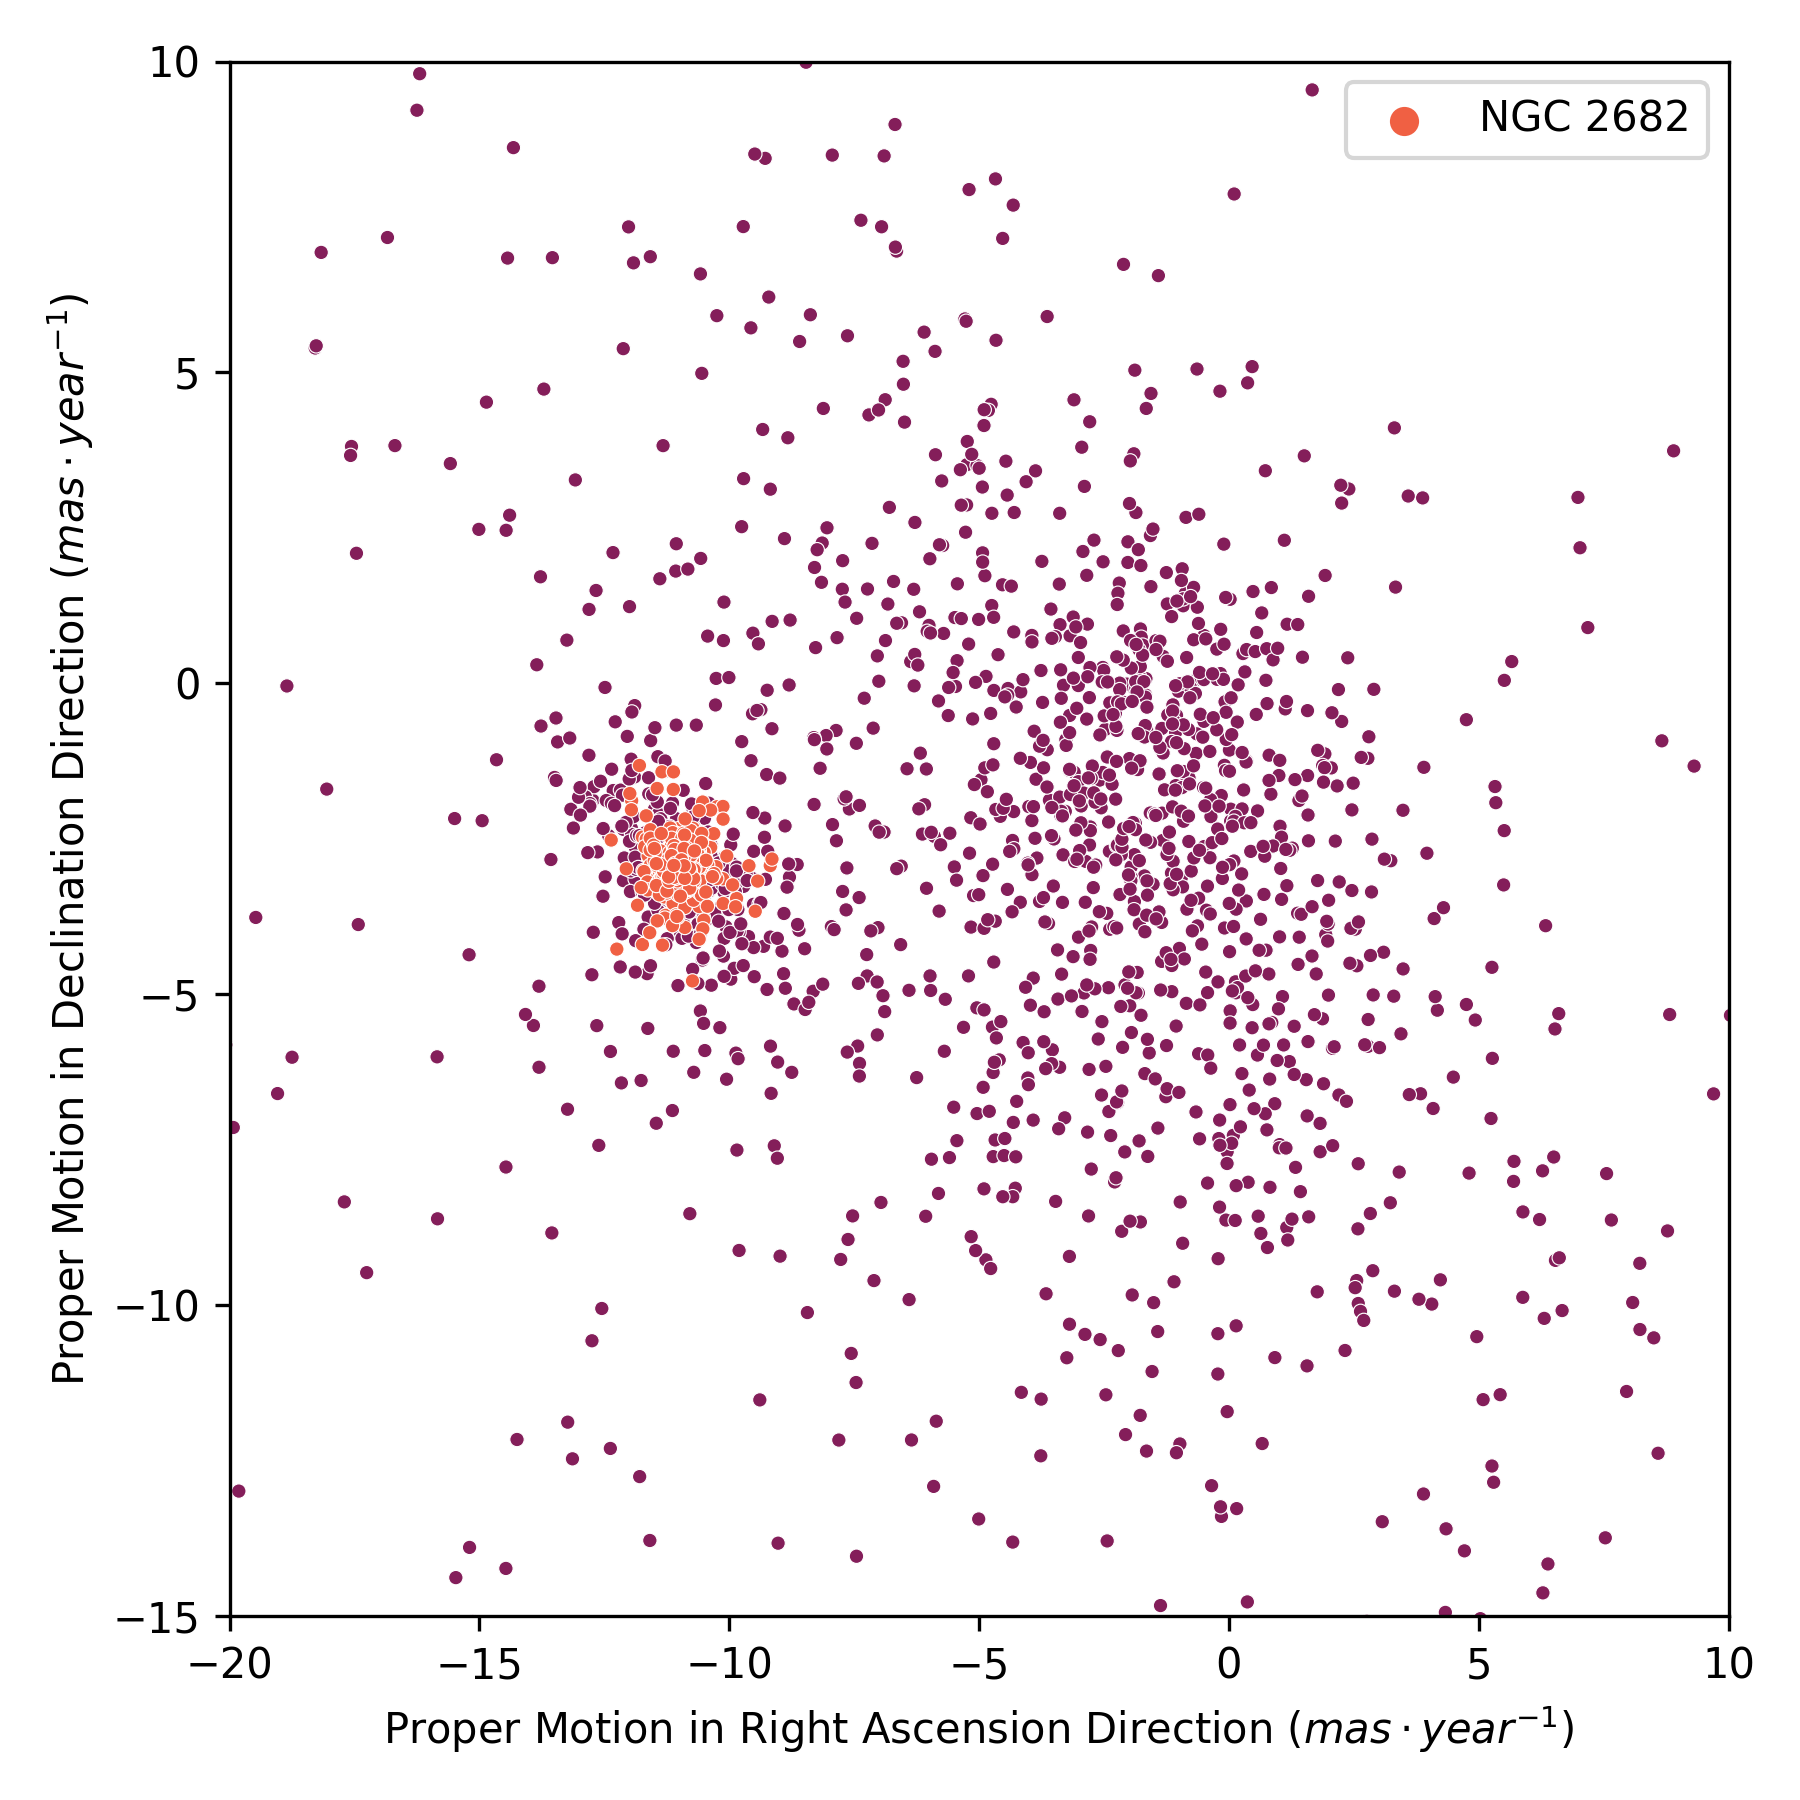
\includegraphics[width=\textwidth]{../figures/ngc_2682/pm_ngc_2682.png}
    \end{subfigure}
    \hfill
    \begin{subfigure}[t]{0.30\textwidth}
      \centering
      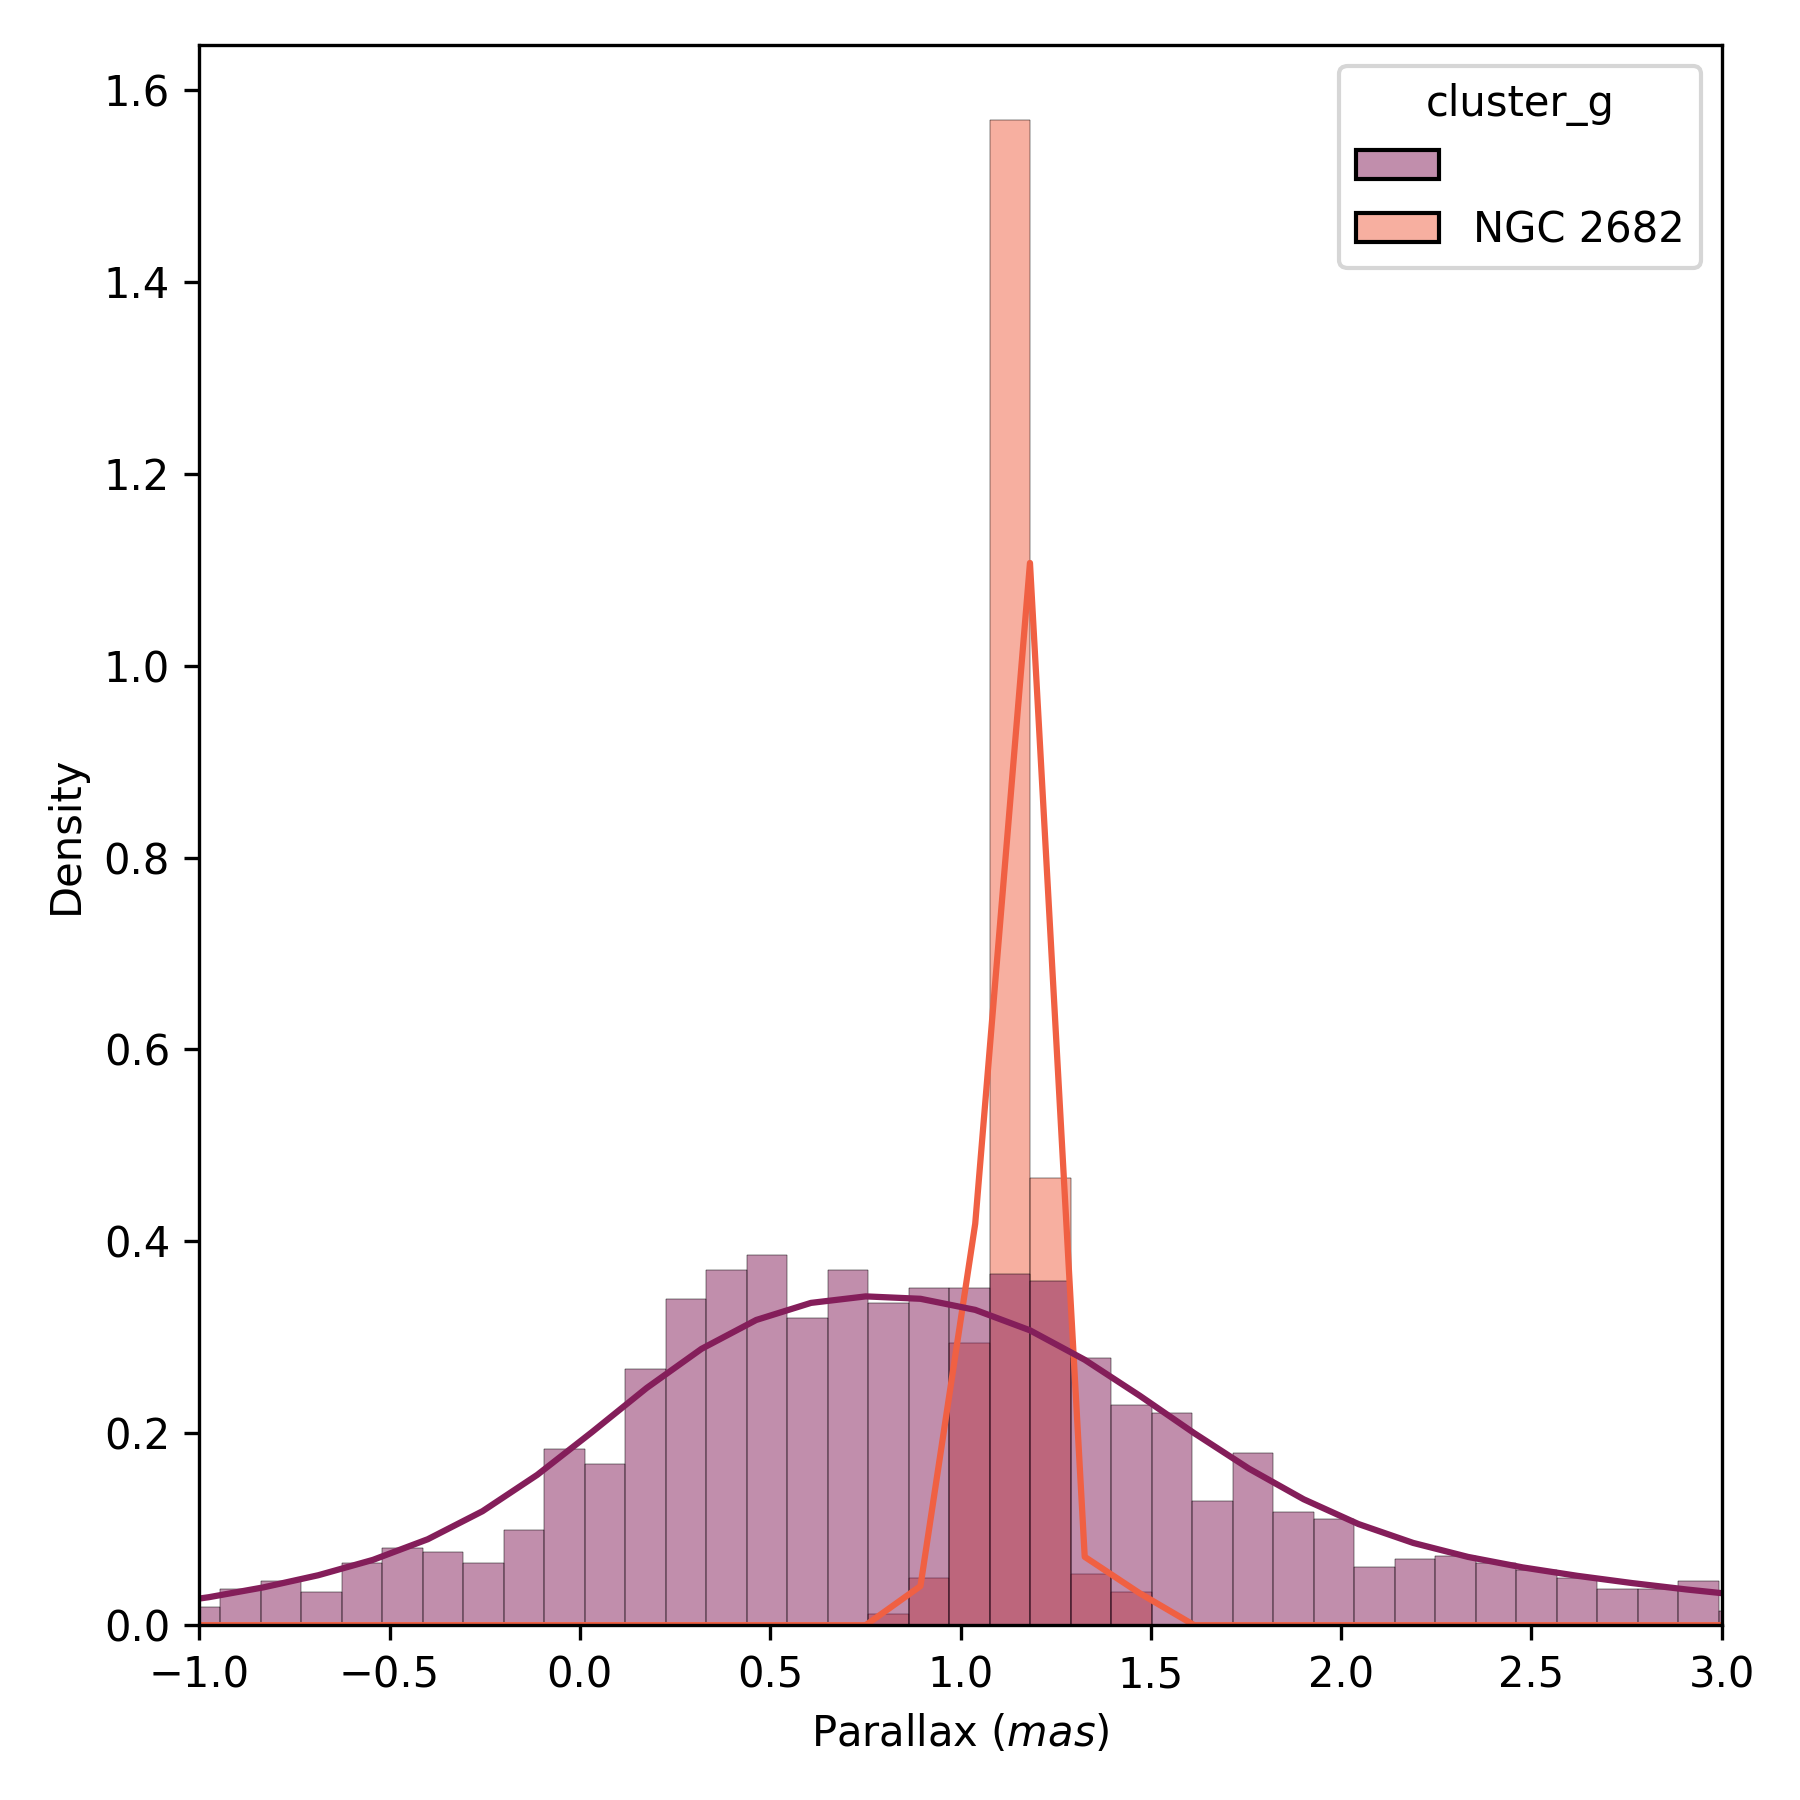
\includegraphics[width=\textwidth]{../figures/ngc_2682/parallax_ngc_2682.png}
    \end{subfigure}
    \hfill
    \begin{subfigure}[t]{0.30\textwidth}
      \centering
      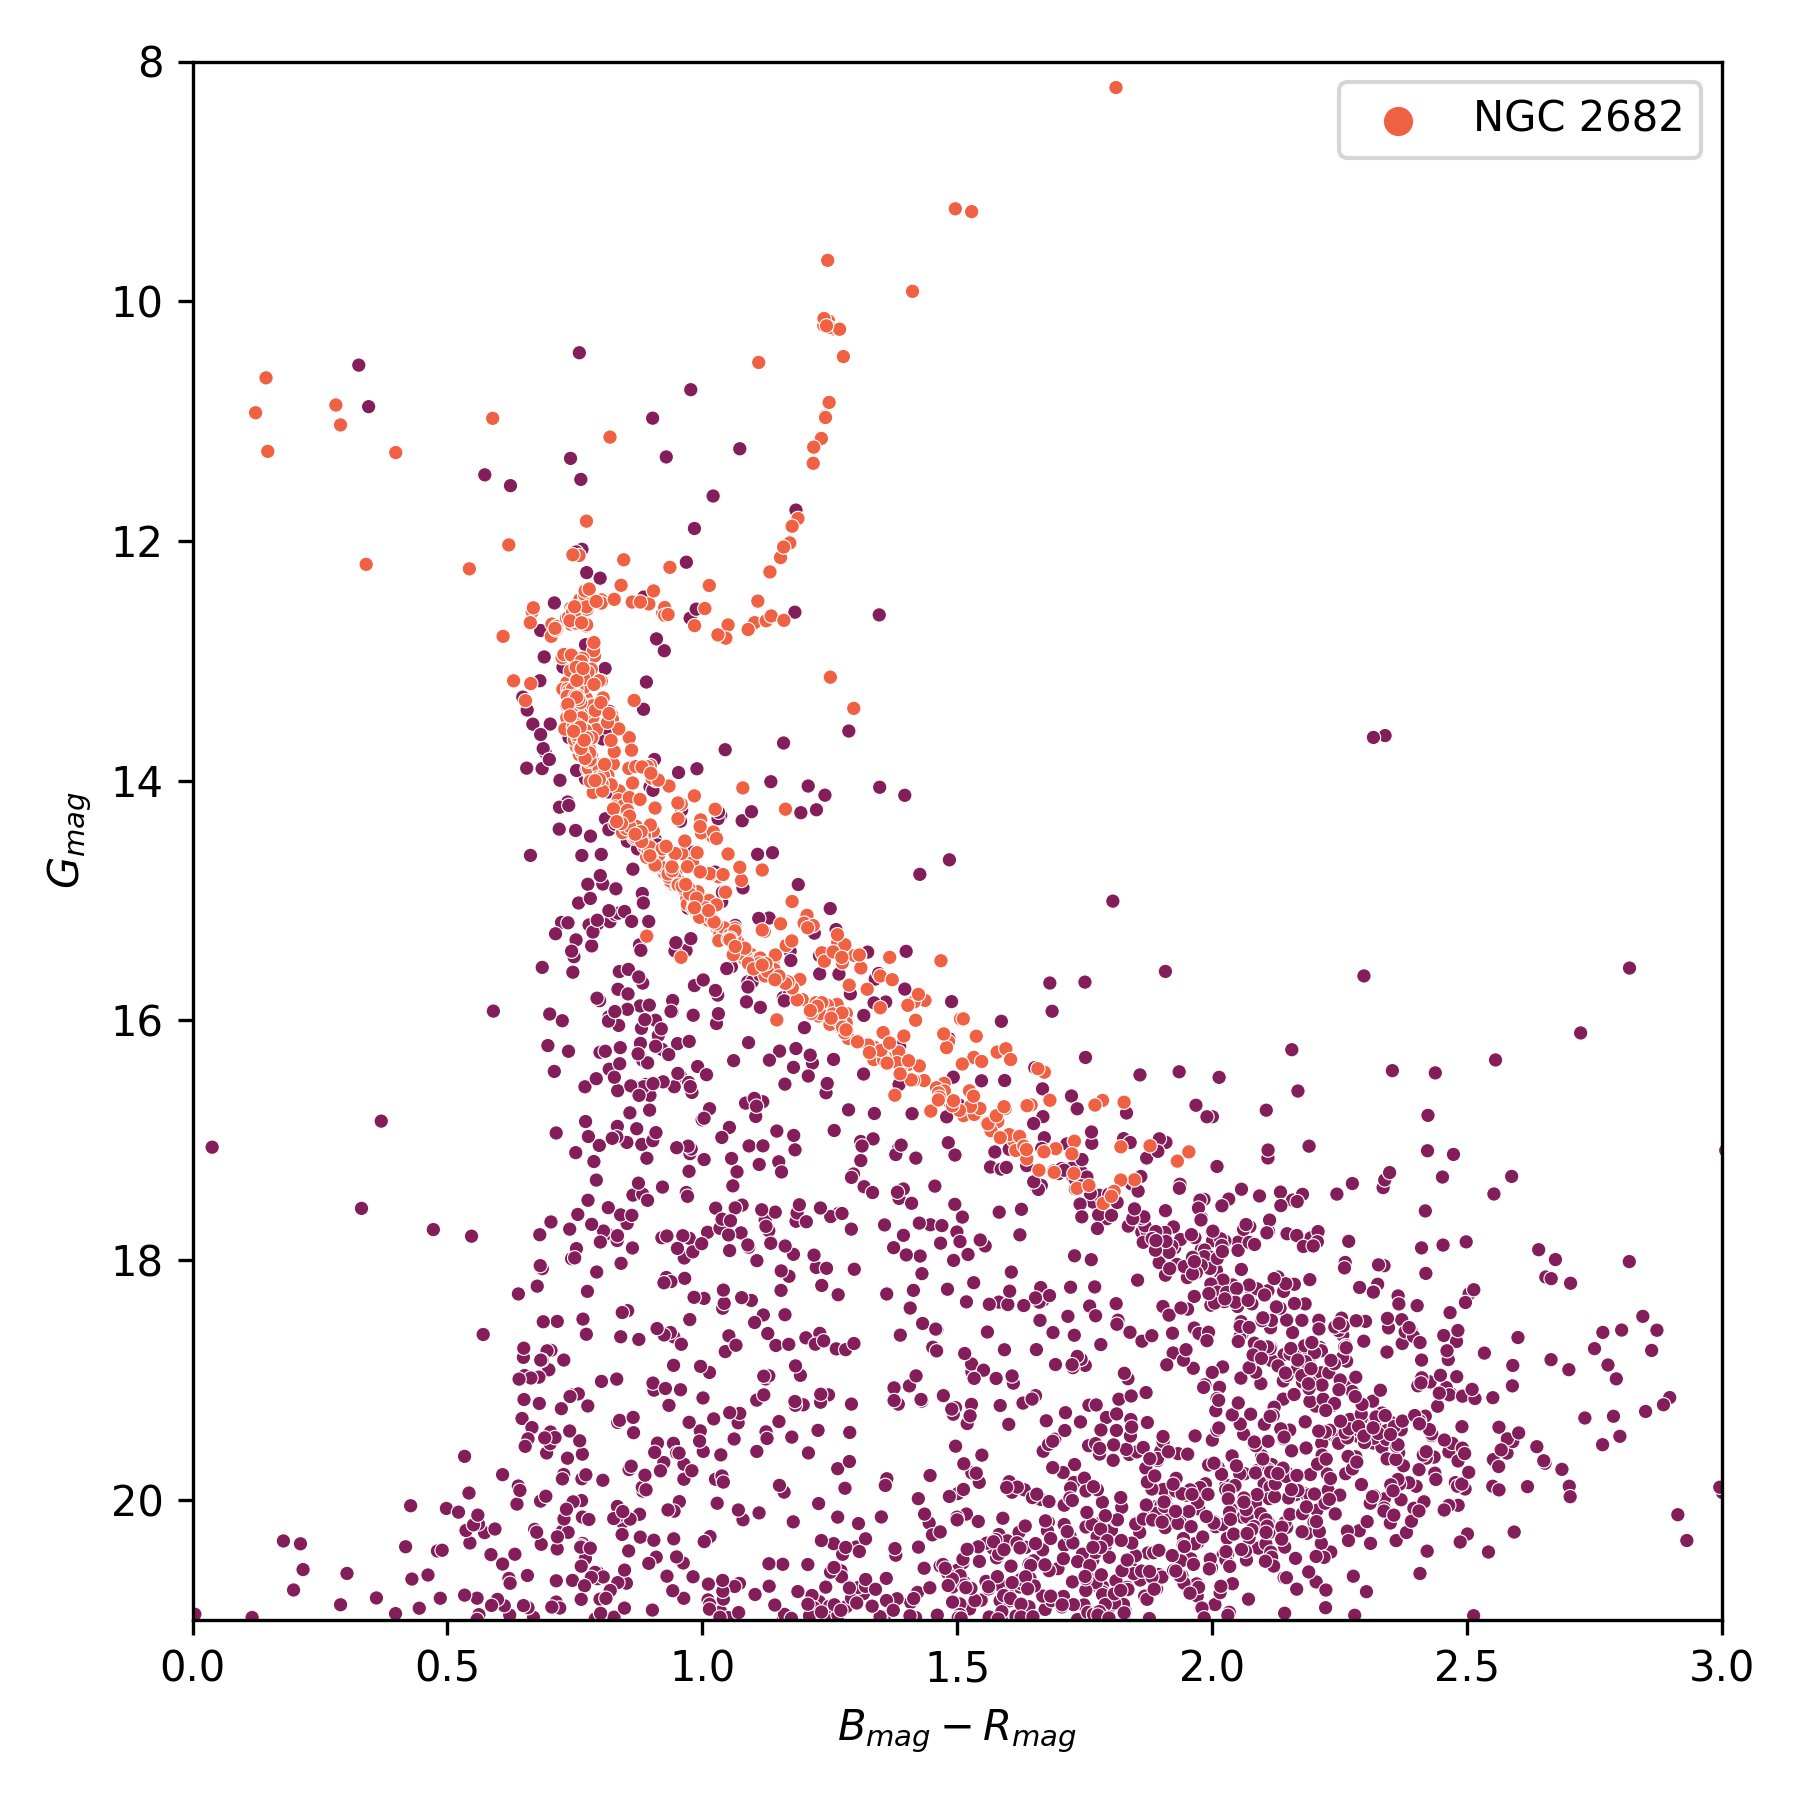
\includegraphics[width=\textwidth]{../figures/ngc_2682/hr_diagram_ngc_2682.png}
    \end{subfigure}
  \end{subfigure}
  \centering
  \begin{subfigure}{\columnwidth}
    \centering
    \begin{subfigure}[t]{0.30\textwidth}
      \centering
      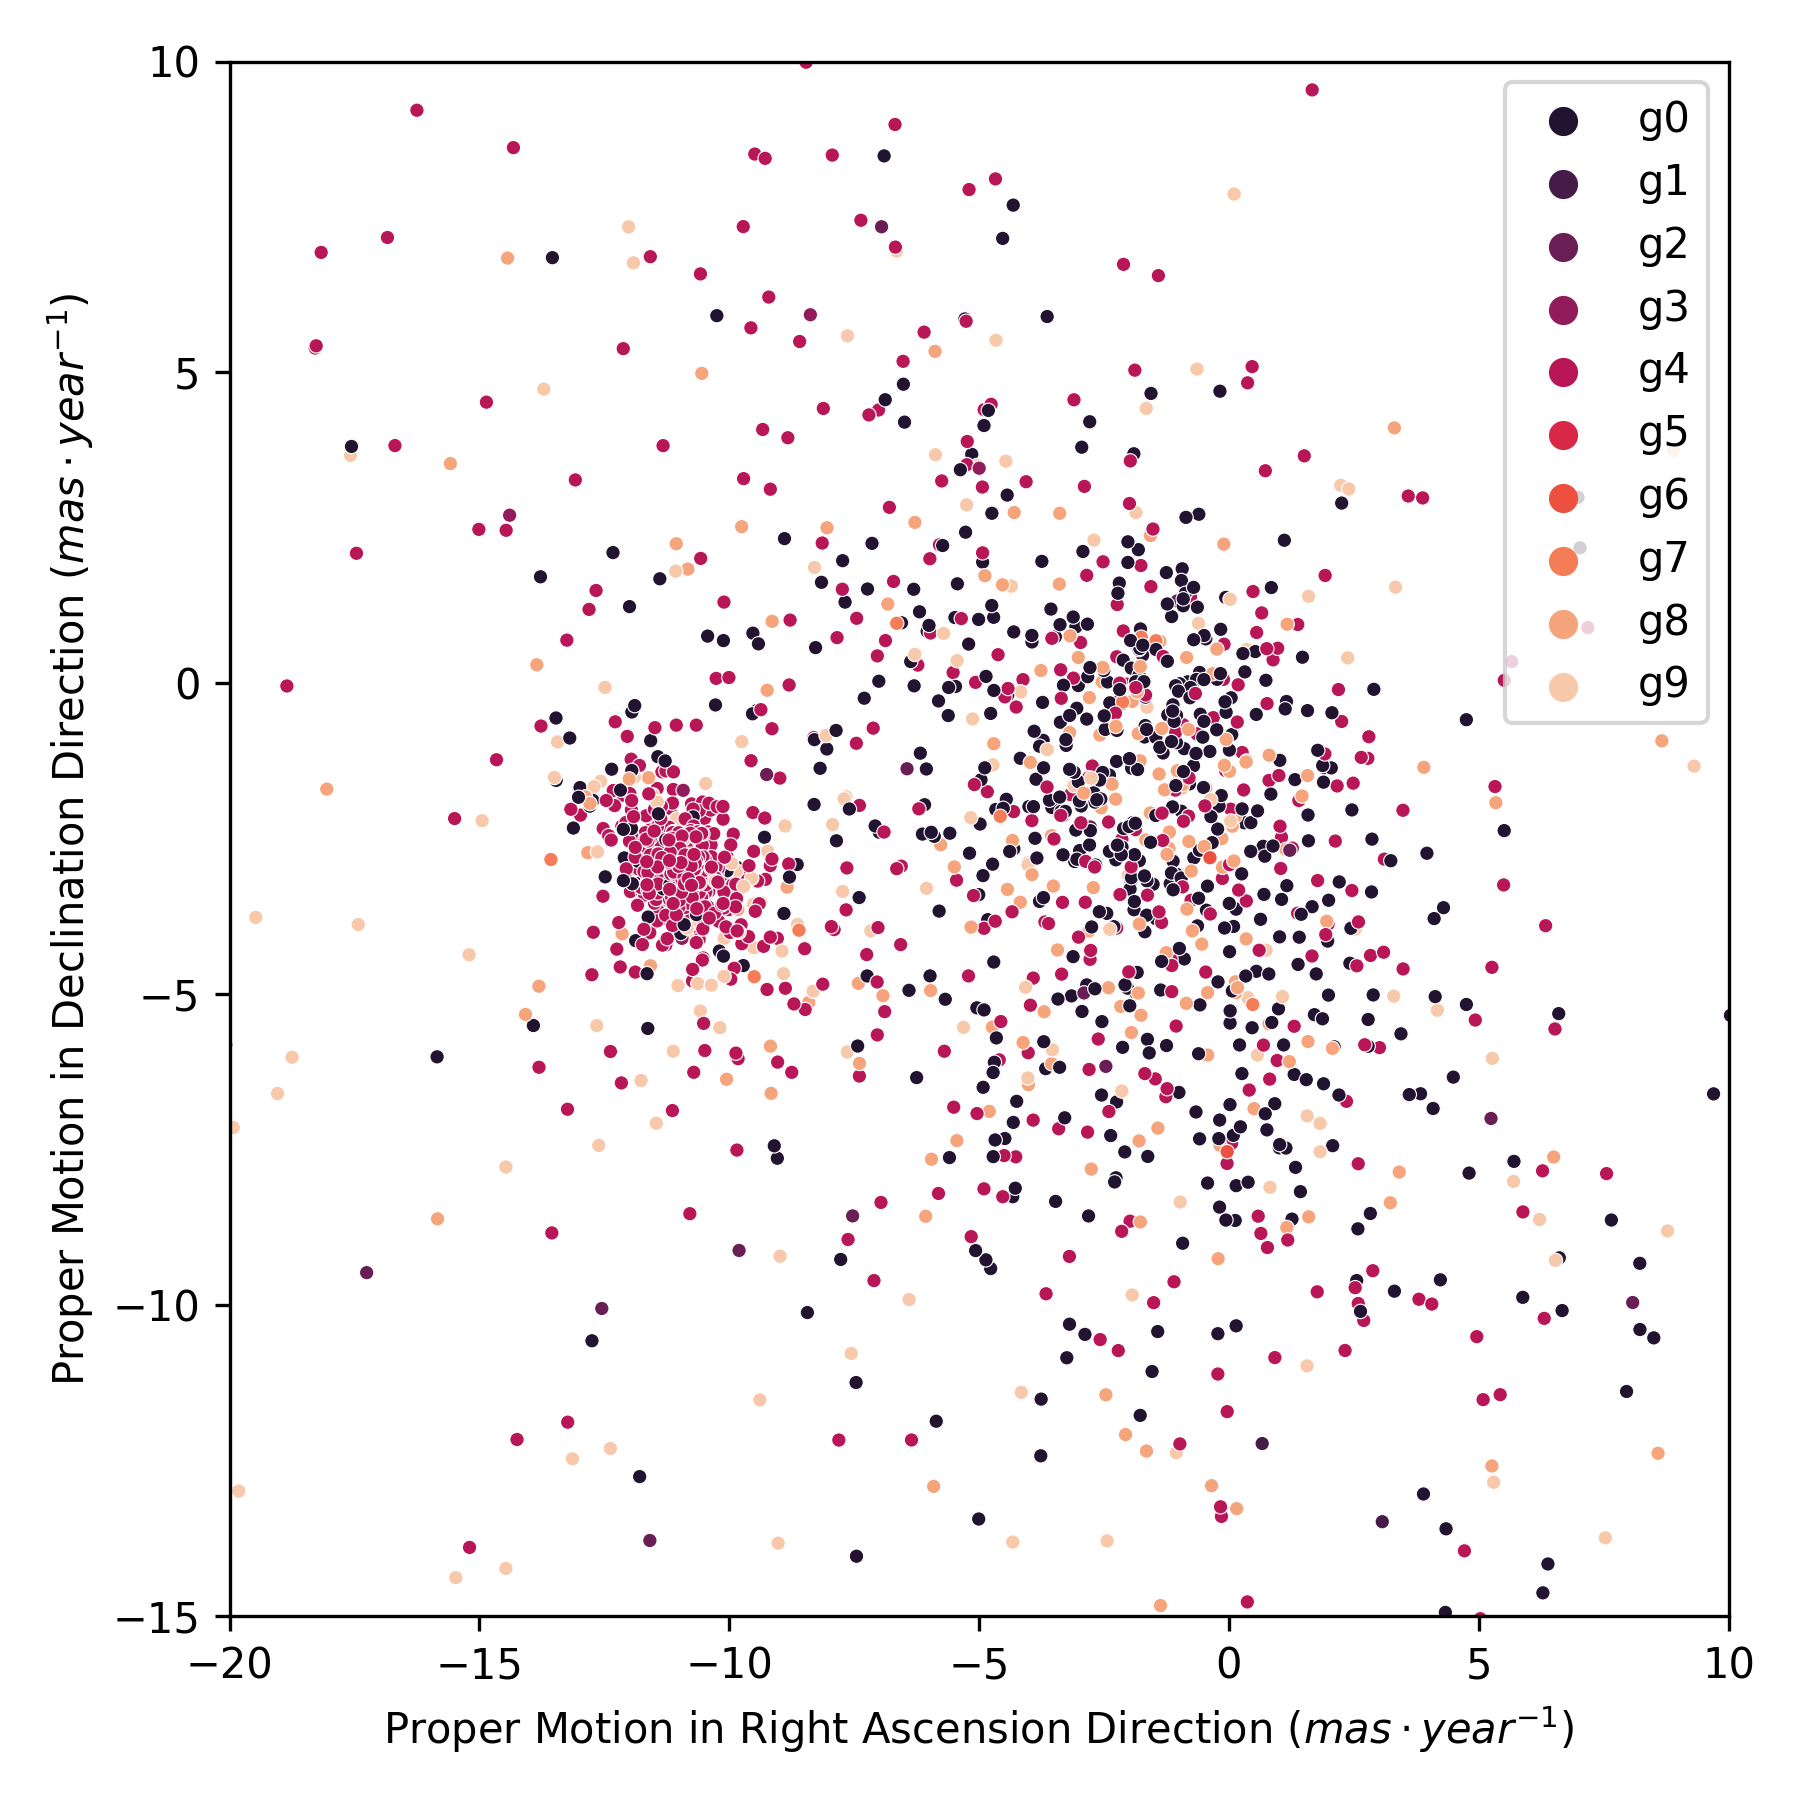
\includegraphics[width=\textwidth]{../figures/ngc_2682/kmeans_pm_ngc_2682.png}
    \end{subfigure}
    \hfill
    \begin{subfigure}[t]{0.30\textwidth}
      \centering
      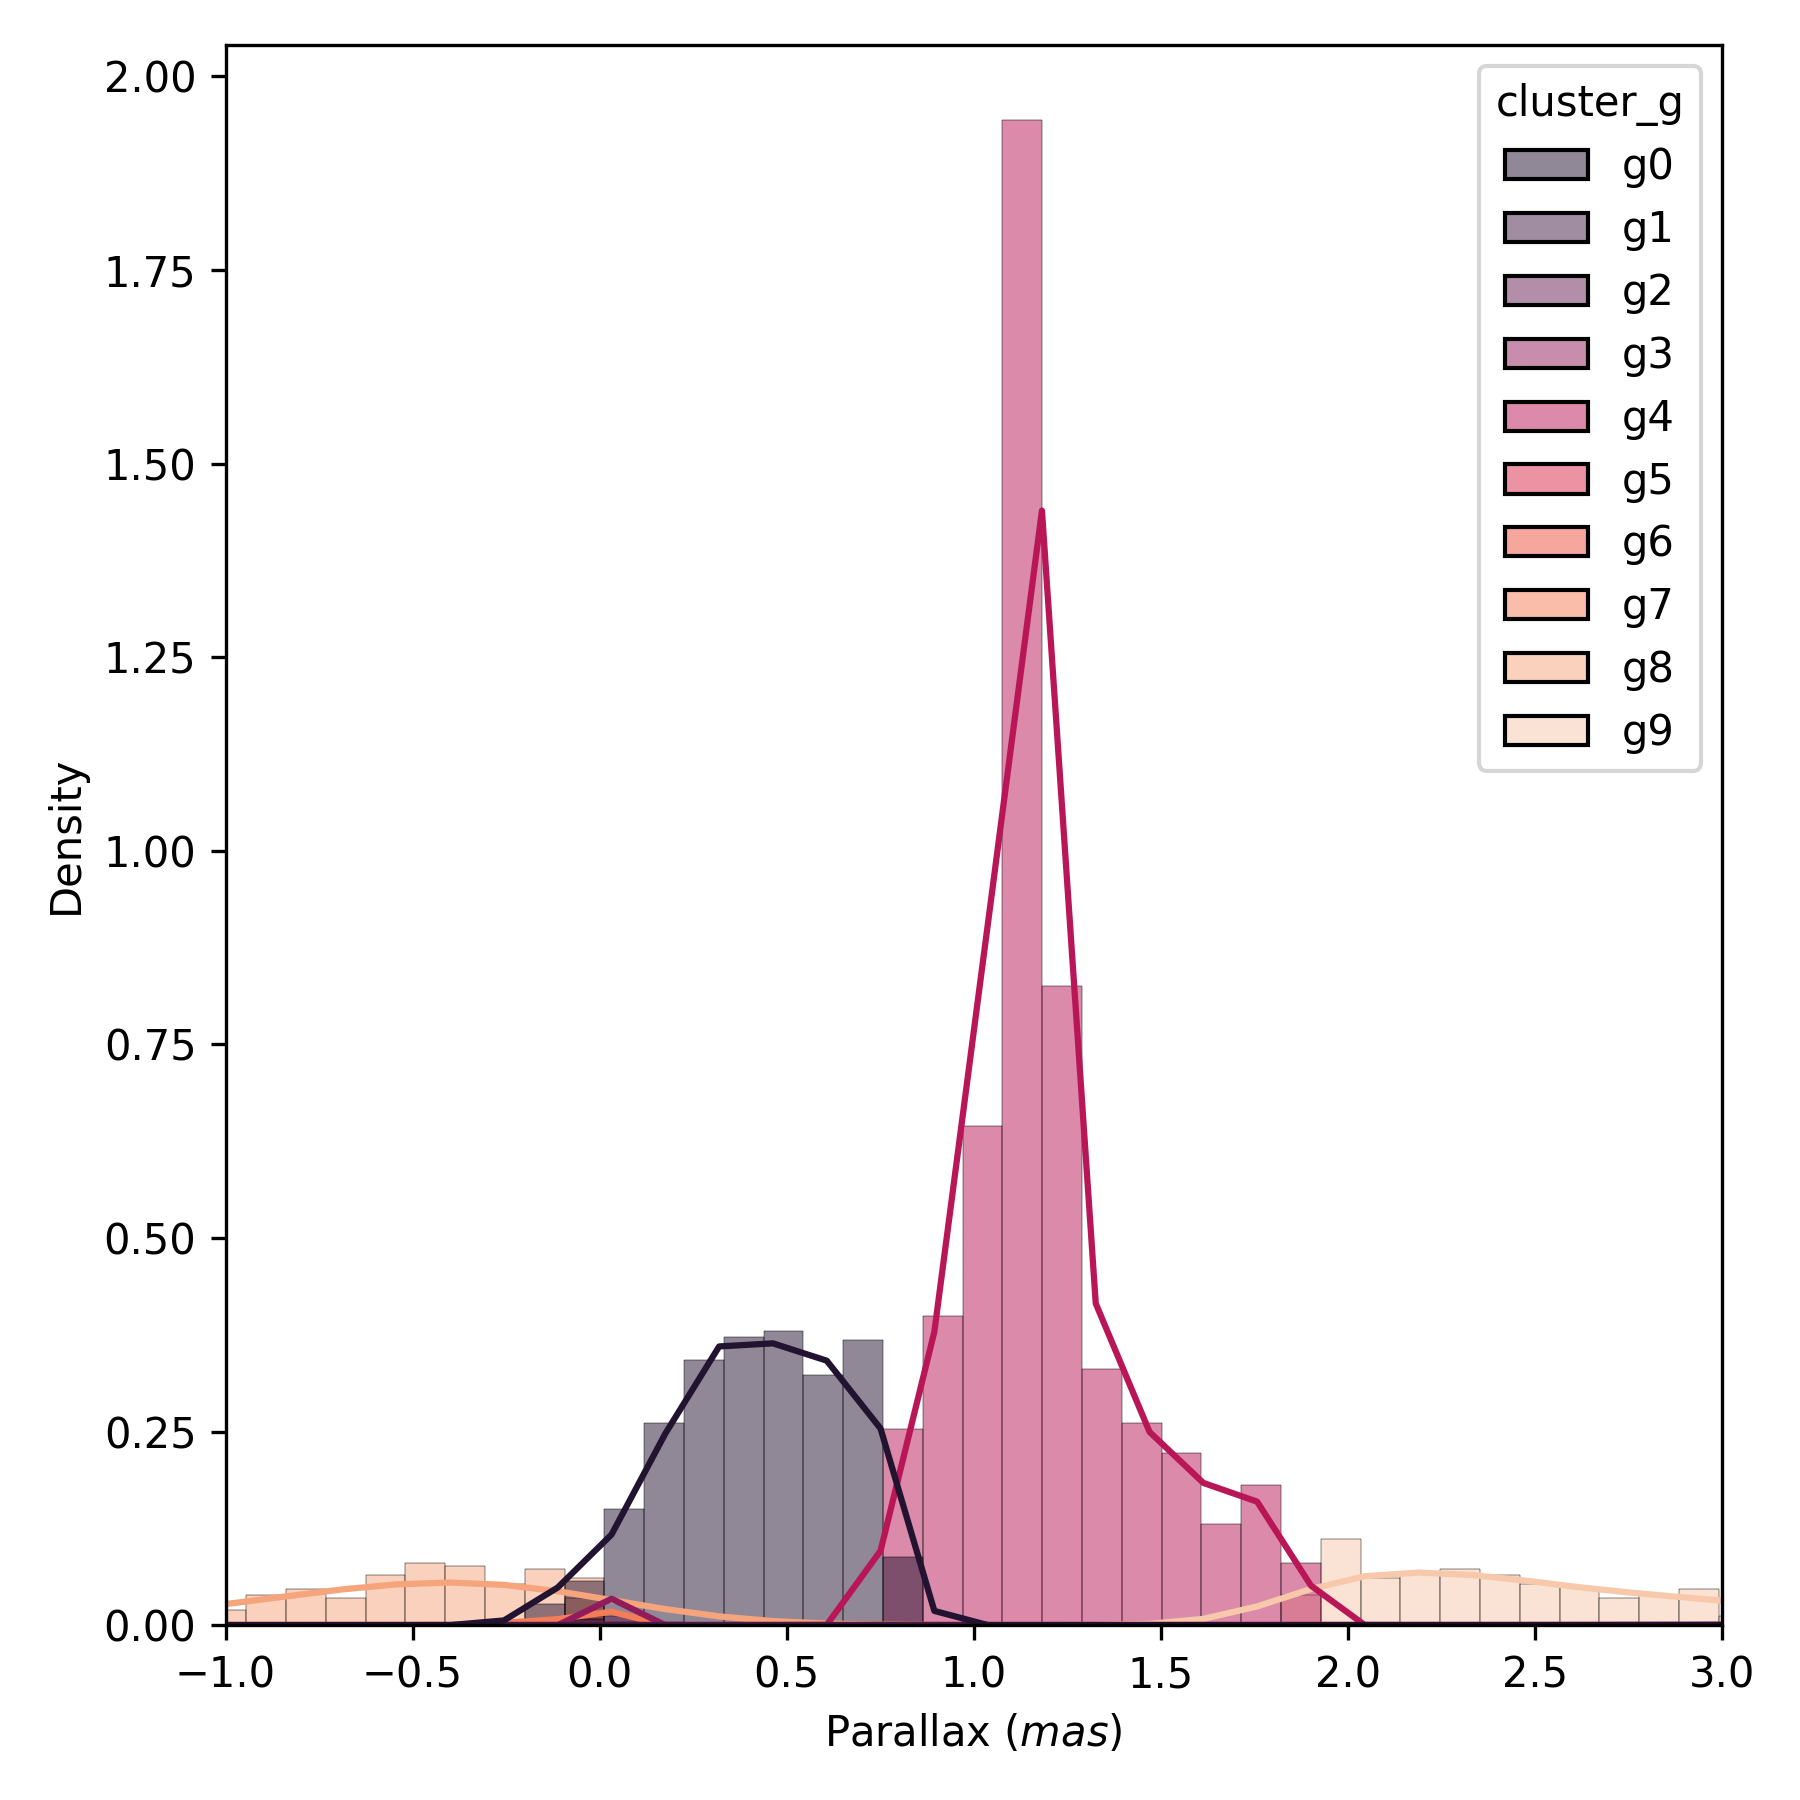
\includegraphics[width=\textwidth]{../figures/ngc_2682/kmeans_parallax_ngc_2682.png}
    \end{subfigure}
    \hfill
    \begin{subfigure}[t]{0.30\textwidth}
      \centering
      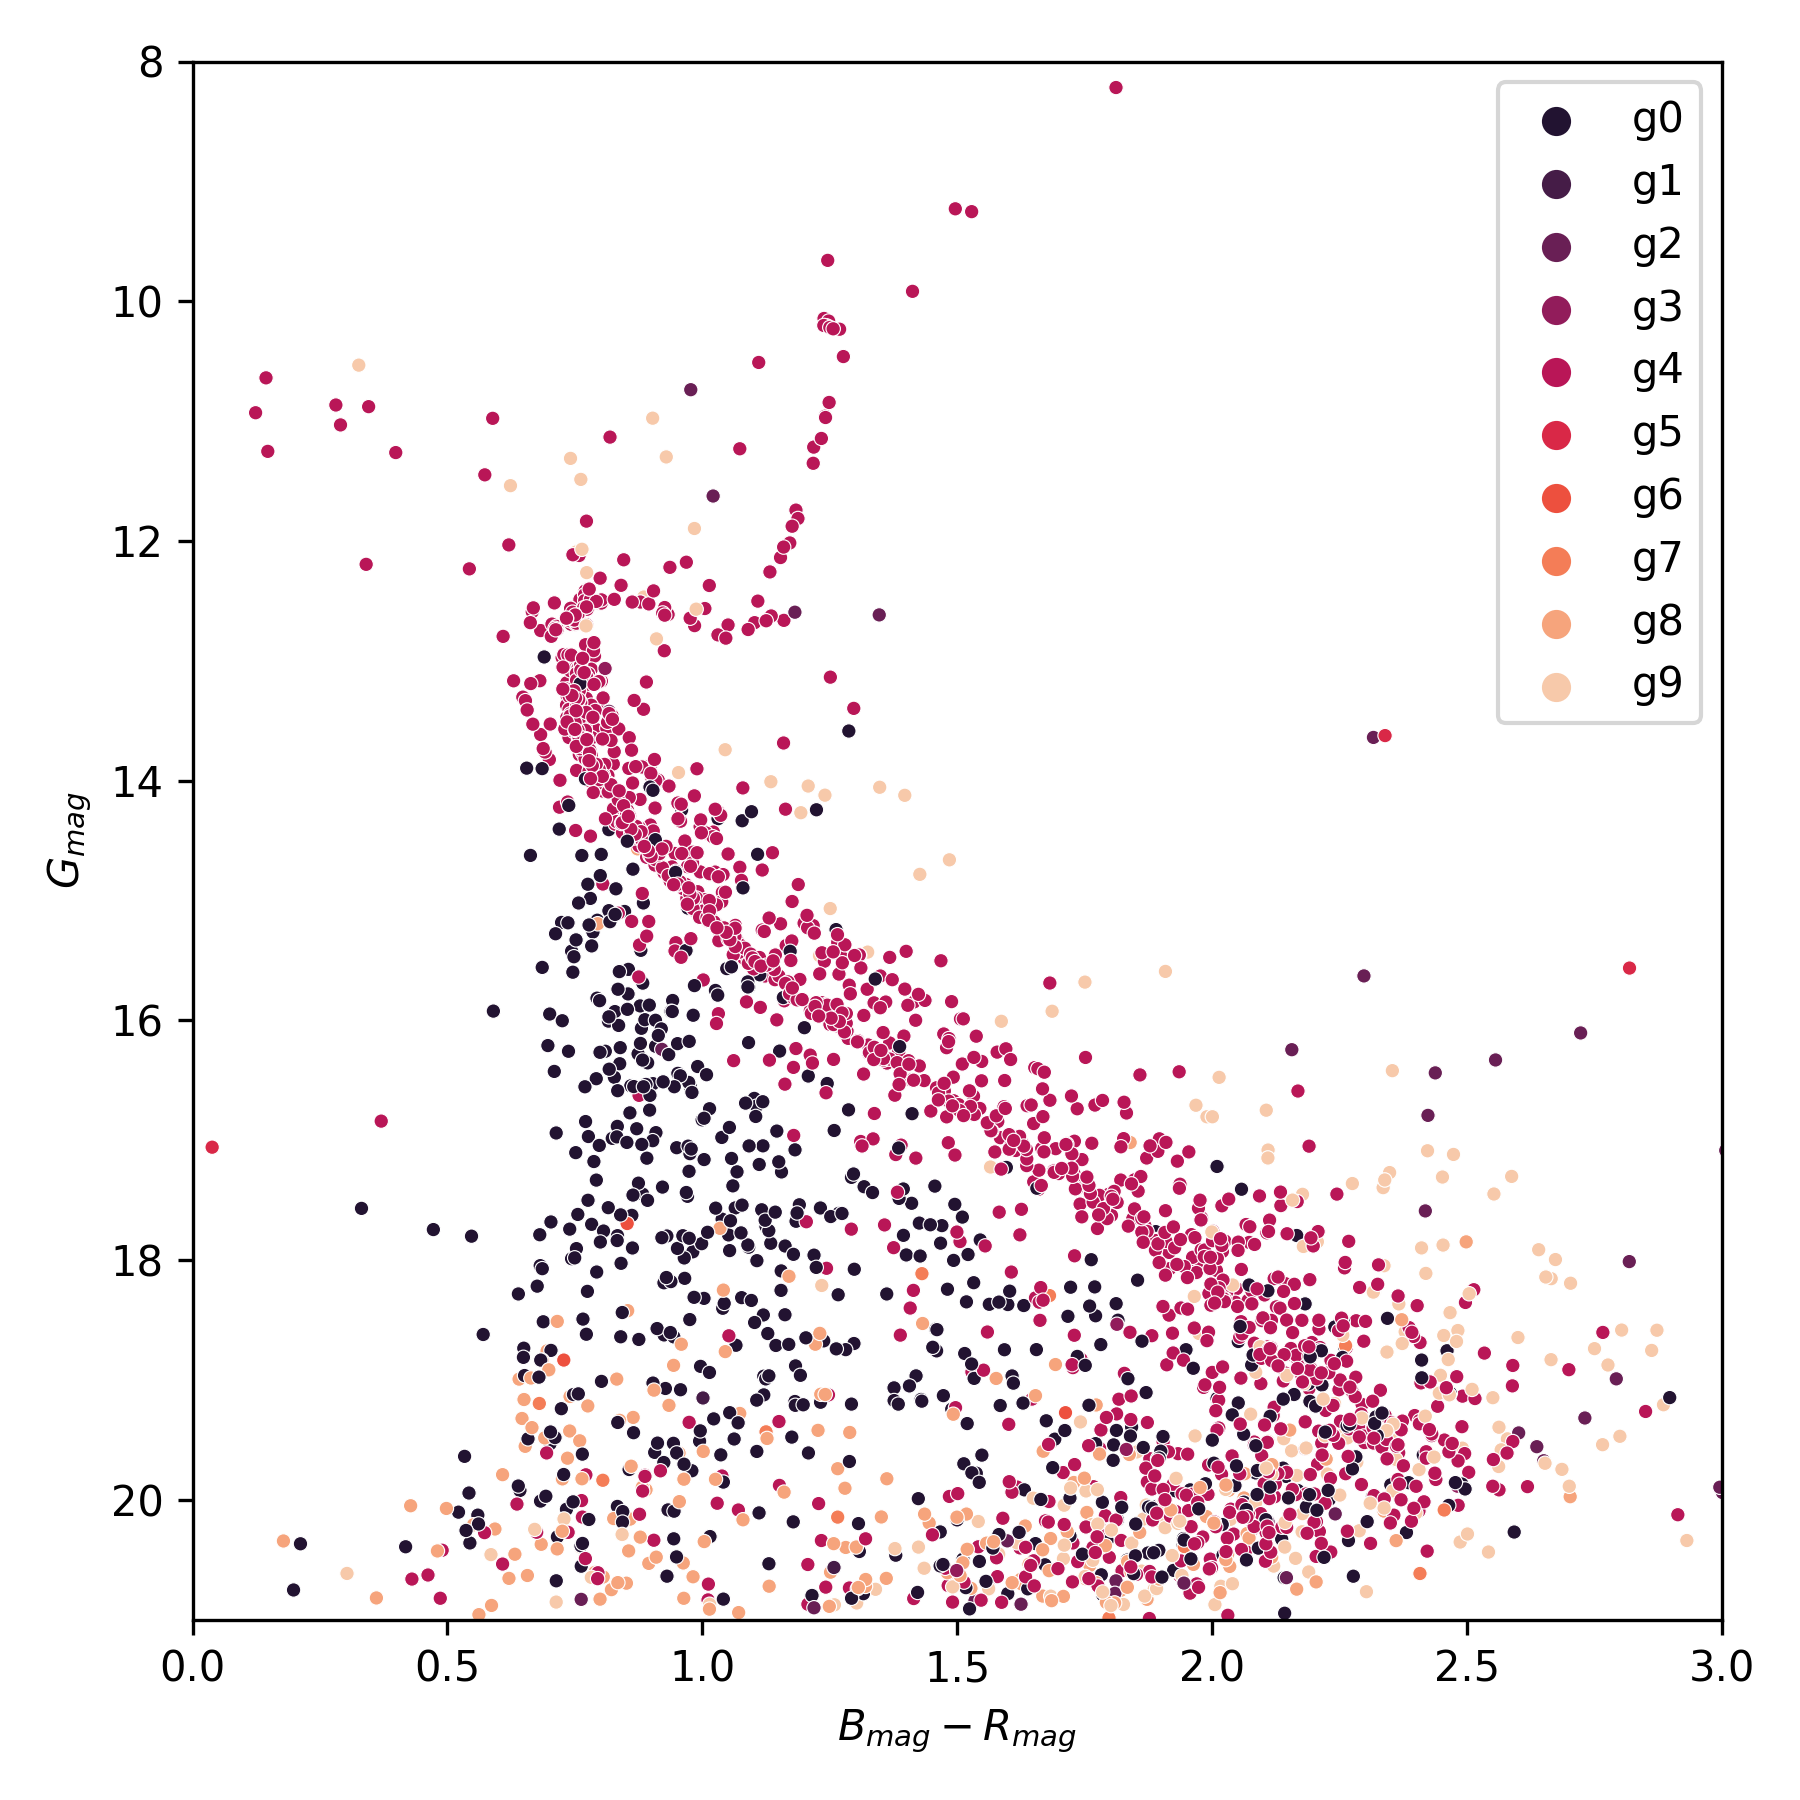
\includegraphics[width=\textwidth]{../figures/ngc_2682/kmeans_hr_diagram_ngc_2682.png}
    \end{subfigure}
  \end{subfigure}
  \caption{NGC 2682 K-Means characterization.
           Top row corresponds to Clusterix+TOPCAT characterization,
           while bottom row shows K-Means results identifying
           NGC 2682 as cluster \emph{g4}.}
  \label{fig:app_result_ngc_2682_clusterix_kmeans}
\end{figure}

Figure \ref{fig:app_result_ngc_2682_dec} shows the groups found using
the DEC model (first row) and the DEC model filtered (second row).
The cluster of interest is the group \emph{g2}.

\begin{figure}[htbp]
  \centering
  \begin{subfigure}{\columnwidth}
    \centering
    \begin{subfigure}[t]{0.30\textwidth}
      \centering
      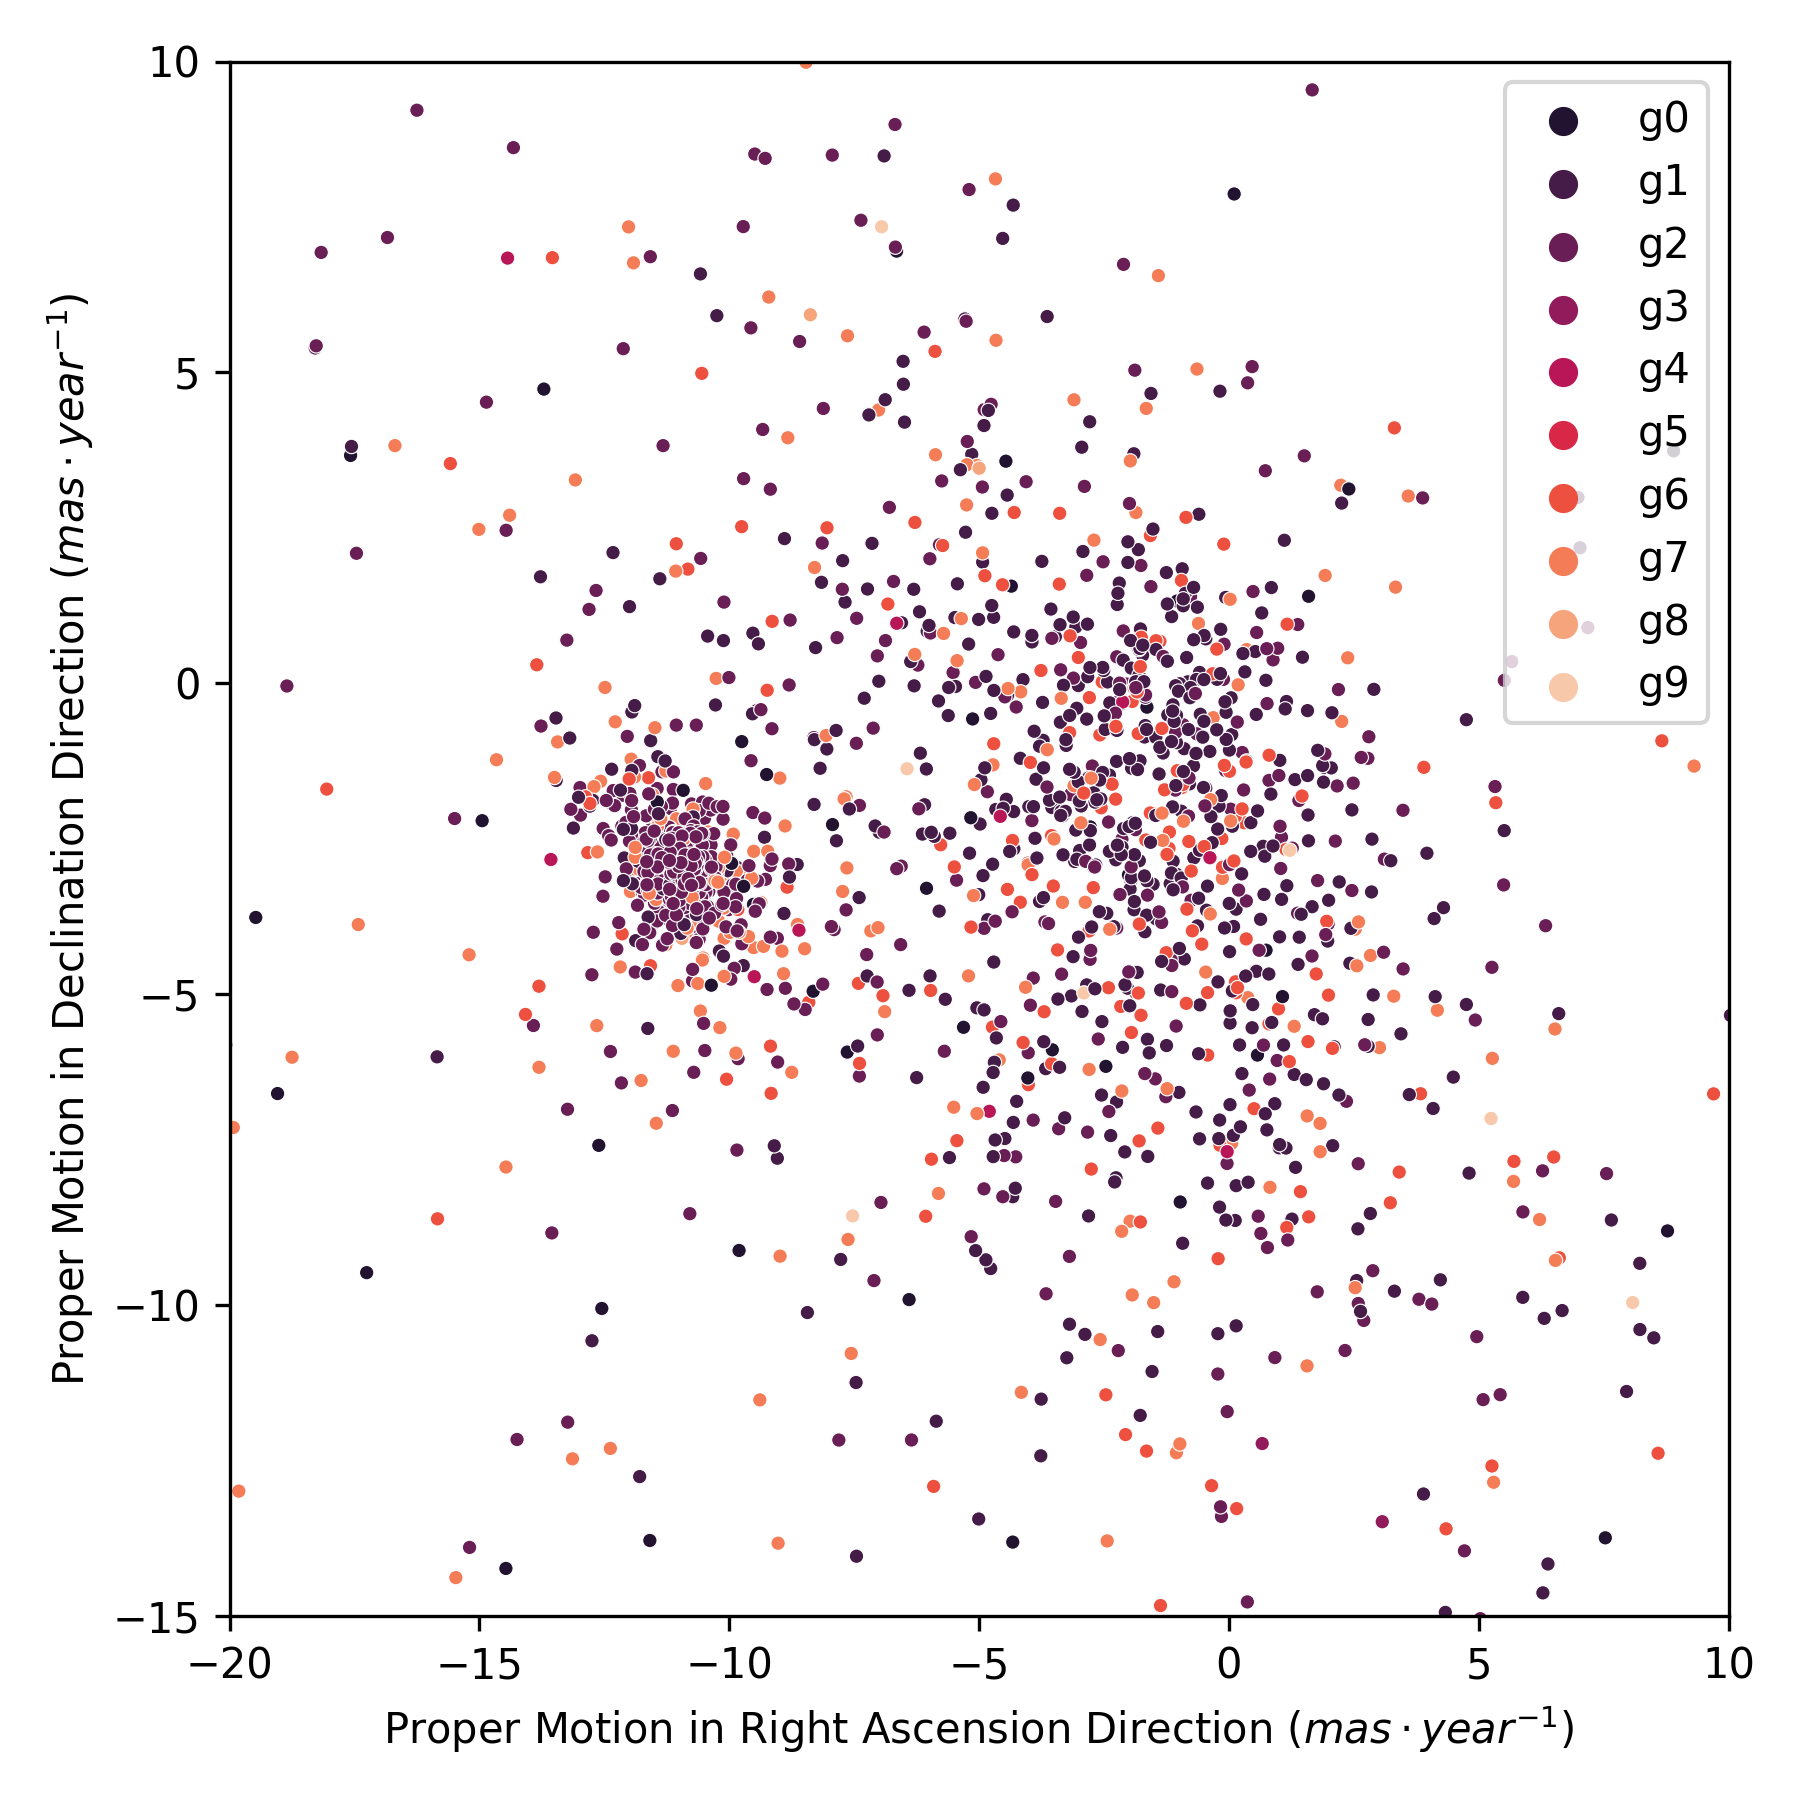
\includegraphics[width=\textwidth]{../figures/ngc_2682/dec_pm_ngc_2682.png}
    \end{subfigure}
    \hfill
    \begin{subfigure}[t]{0.30\textwidth}
      \centering
      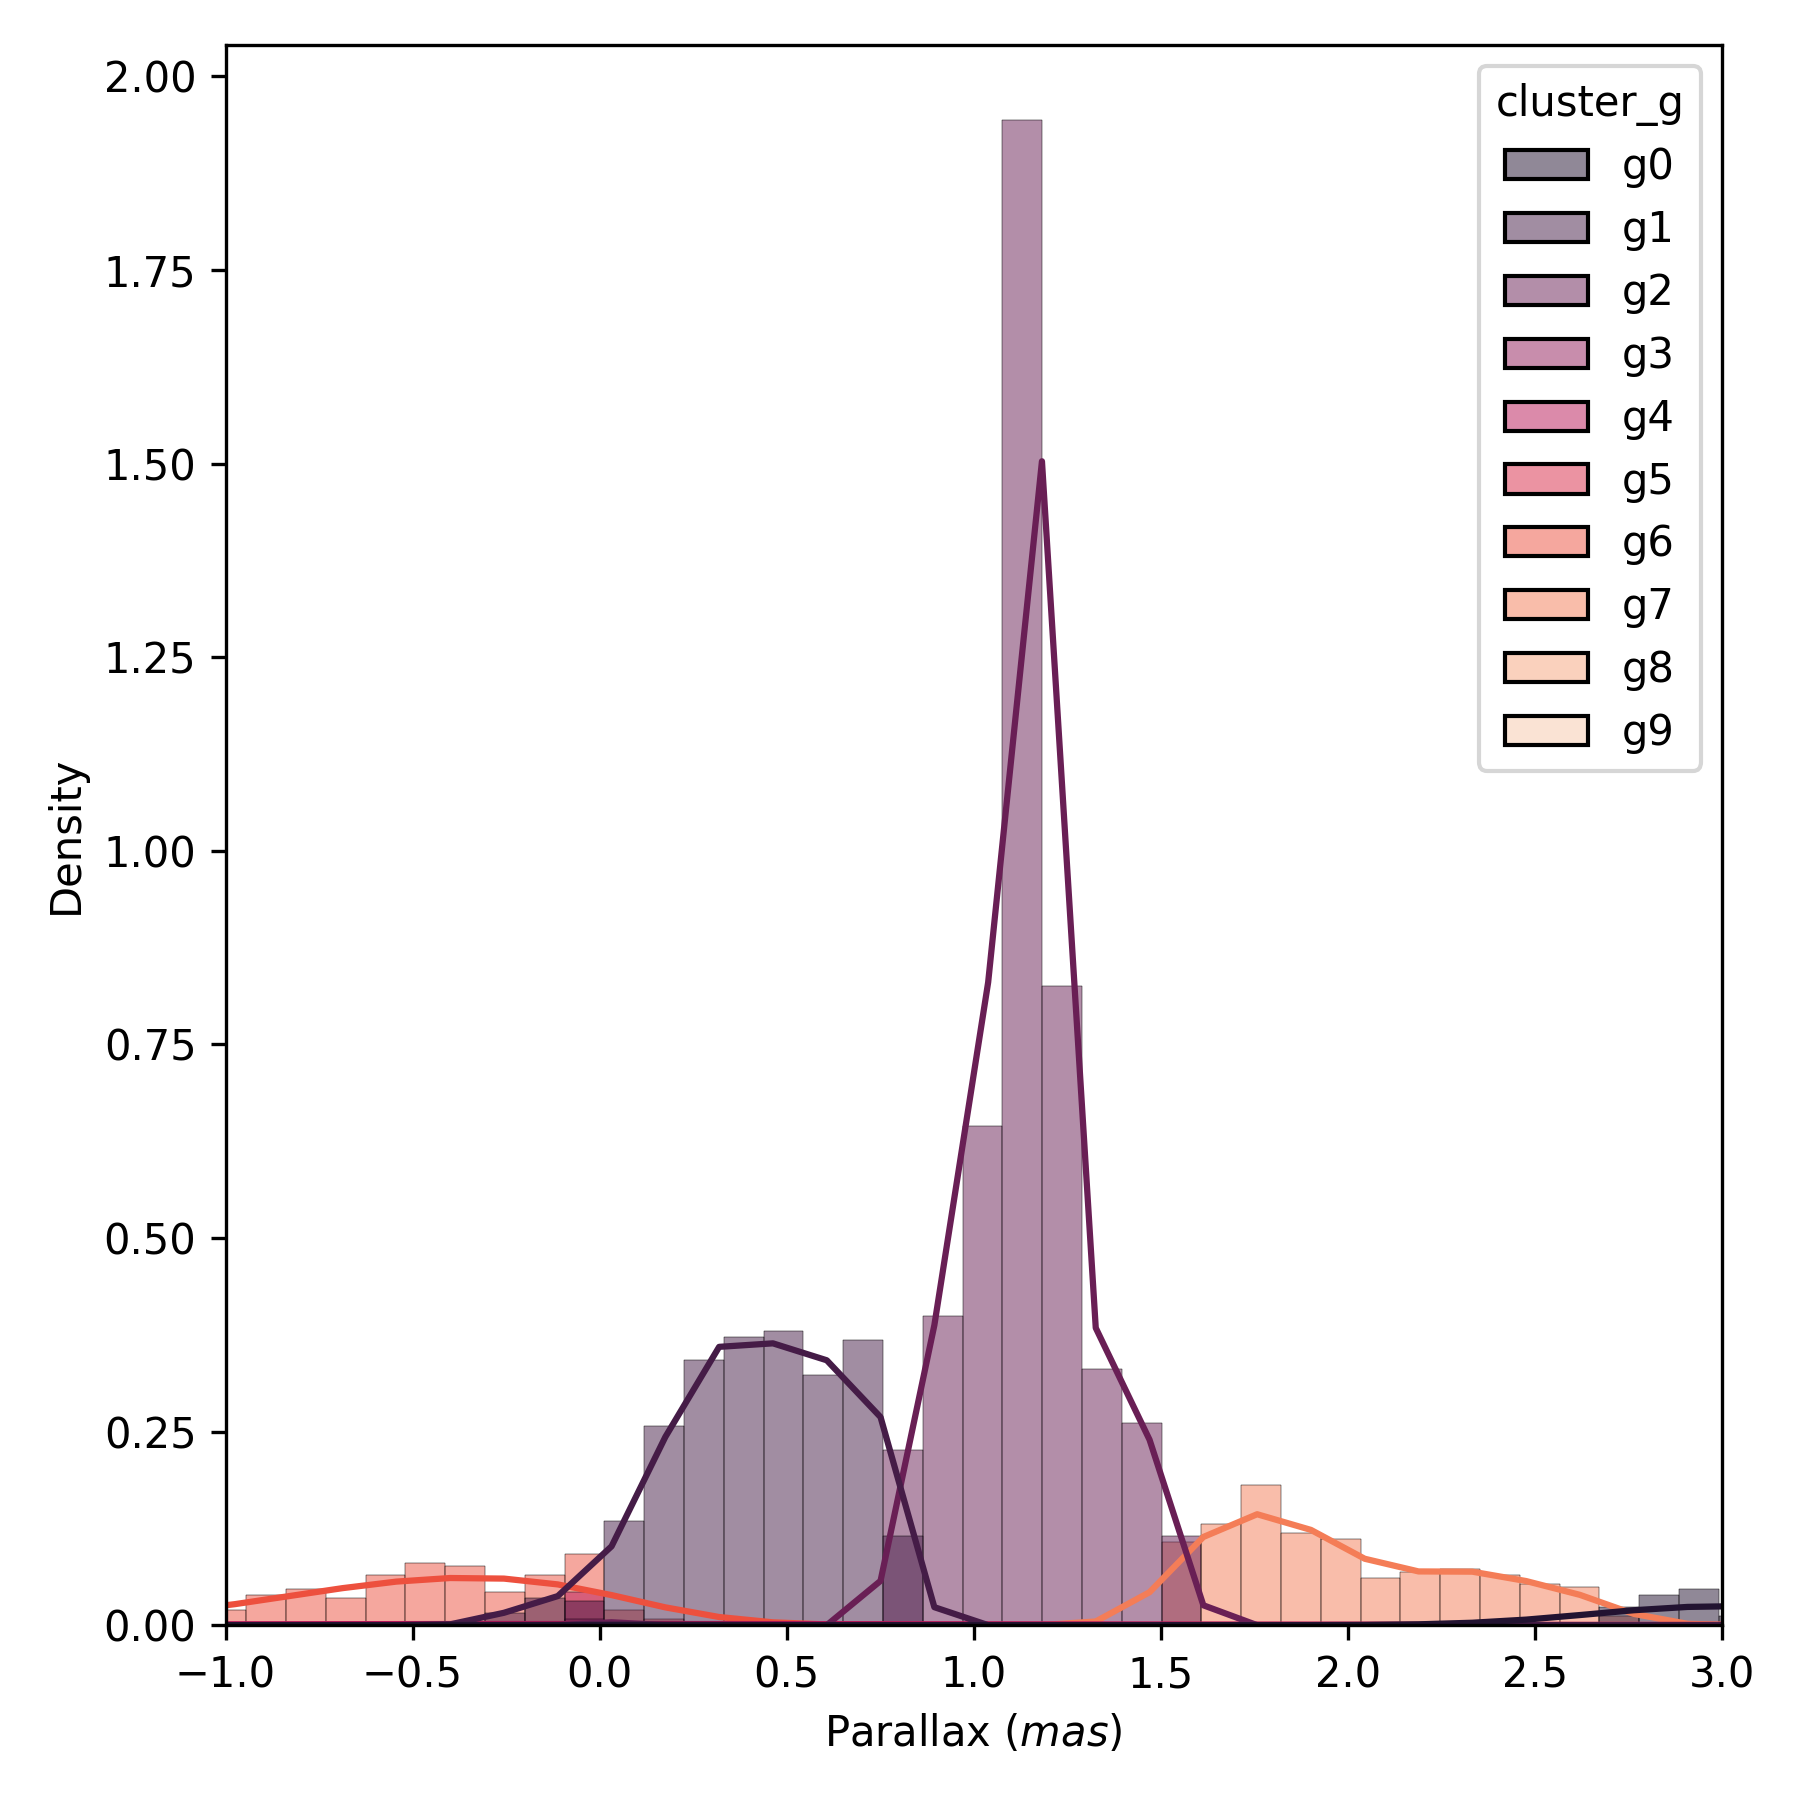
\includegraphics[width=\textwidth]{../figures/ngc_2682/dec_parallax_ngc_2682.png}
    \end{subfigure}
    \hfill
    \begin{subfigure}[t]{0.30\textwidth}
      \centering
      \includegraphics[width=\textwidth]{../figures/ngc_2682/dec_hr_diagram_ngc_2682.png}
    \end{subfigure}
  \end{subfigure}
  \centering
  \begin{subfigure}{\columnwidth}
    \centering
    \begin{subfigure}[t]{0.30\textwidth}
      \centering
      \includegraphics[width=\textwidth]{../figures/ngc_2682/dec_pm_filtered_ngc_2682.png}
    \end{subfigure}
    \hfill
    \begin{subfigure}[t]{0.30\textwidth}
      \centering
      \includegraphics[width=\textwidth]{../figures/ngc_2682/dec_parallax_filtered_ngc_2682.png}
    \end{subfigure}
    \hfill
    \begin{subfigure}[t]{0.30\textwidth}
      \centering
      \includegraphics[width=\textwidth]{../figures/ngc_2682/dec_hr_diagram_filtered_ngc_2682.png}
    \end{subfigure}
  \end{subfigure}
  \caption{NGC 2682 is identified as cluster \emph{g2}.
           Top row: DEC --- Bottom row: DEC (filtered)}
  \label{fig:app_result_ngc_2682_dec}
\end{figure}

Table \ref{tab:app_hyperparameters_ngc_2682} shows the
hyperparameters used for characterizing NGC 2682 with DEC method.

\begin{table}[htbp]
  \begin{center}
    \begin{tabular}{l|c}
      \textbf{Hyperparameter} & \textbf{Value} \\
      \hline
      Number of Clusters & 10 \\
      Clustering Layer & $\left[ 50, 50, 40 \right]$ \\
      Kernel Initializer Seed & 0 \\
      Quantil Threshold & 0.1 \\
    \end{tabular}
    \caption{NGC 2682 DEC hyperparameters.}
    \label{tab:app_hyperparameters_ngc_2682}
  \end{center}
\end{table}

\subsection{MELOTTE 22}
\label{sec:melotte22}

\begin{figure}[htbp]
  \centering
  \begin{subfigure}{\columnwidth}
    \centering
    \begin{subfigure}[t]{0.30\textwidth}
      \centering
      \includegraphics[width=\textwidth]{../figures/melotte_22/pm_melotte_22.png}
    \end{subfigure}
    \hfill
    \begin{subfigure}[t]{0.30\textwidth}
      \centering
      \includegraphics[width=\textwidth]{../figures/melotte_22/parallax_melotte_22.png}
    \end{subfigure}
    \hfill
    \begin{subfigure}[t]{0.30\textwidth}
      \centering
      \includegraphics[width=\textwidth]{../figures/melotte_22/hr_diagram_melotte_22.png}
    \end{subfigure}
  \end{subfigure}
  \centering
  \begin{subfigure}{\columnwidth}
    \centering
    \begin{subfigure}[t]{0.30\textwidth}
      \centering
      \includegraphics[width=\textwidth]{../figures/melotte_22/kmeans_pm_melotte_22.png}
    \end{subfigure}
    \hfill
    \begin{subfigure}[t]{0.30\textwidth}
      \centering
      \includegraphics[width=\textwidth]{../figures/melotte_22/kmeans_parallax_melotte_22.png}
    \end{subfigure}
    \hfill
    \begin{subfigure}[t]{0.30\textwidth}
      \centering
      \includegraphics[width=\textwidth]{../figures/melotte_22/kmeans_hr_diagram_melotte_22.png}
    \end{subfigure}
  \end{subfigure}
  \caption{Melotte 22 characterization.
           Top row: Clusterix+TOPCAT. Bottom row: K-Means.
           Melotte 22 is labeled as cluster \emph{g1}.}
  \label{fig:app_result_melotte_22_clusterix_kmeans}
\end{figure}

Figure \ref{fig:app_result_melotte_22_clusterix_kmeans} shows Melotte 22
characterized using Clusterix+TOPCAT tools (top row) and the characterization
made by K-Means (bottom row) showing nine clusters. Melotte 22 is labeled as
group \emph{g1}.

Figure \ref{fig:app_result_melotte_22_dec} shows the groups found using
DEC model (first row) and DEC model filtered (second row).
Melotte 22 is labeled as group \emph{g2} by DEC model.

\begin{figure}[htbp]
  \centering
  \begin{subfigure}{\columnwidth}
    \centering
    \begin{subfigure}[t]{0.30\textwidth}
      \centering
      \includegraphics[width=\textwidth]{../figures/melotte_22/dec_pm_melotte_22.png}
    \end{subfigure}
    \hfill
    \begin{subfigure}[t]{0.30\textwidth}
      \centering
      \includegraphics[width=\textwidth]{../figures/melotte_22/dec_parallax_melotte_22.png}
    \end{subfigure}
    \hfill
    \begin{subfigure}[t]{0.30\textwidth}
      \centering
      \includegraphics[width=\textwidth]{../figures/melotte_22/dec_hr_diagram_melotte_22.png}
    \end{subfigure}
  \end{subfigure}
  \centering
  \begin{subfigure}{\columnwidth}
    \centering
    \begin{subfigure}[t]{0.30\textwidth}
      \centering
      \includegraphics[width=\textwidth]{../figures/melotte_22/dec_pm_filtered_melotte_22.png}
    \end{subfigure}
    \hfill
    \begin{subfigure}[t]{0.30\textwidth}
      \centering
      \includegraphics[width=\textwidth]{../figures/melotte_22/dec_parallax_filtered_melotte_22.png}
    \end{subfigure}
    \hfill
    \begin{subfigure}[t]{0.30\textwidth}
      \centering
      \includegraphics[width=\textwidth]{../figures/melotte_22/dec_hr_diagram_filtered_melotte_22.png}
    \end{subfigure}
  \end{subfigure}
  \caption{Melotte 22 is identified as cluster \emph{g2}.
           Top row: DEC --- Bottom row: DEC (filtered)}
  \label{fig:app_result_melotte_22_dec}
\end{figure}

Table \ref{tab:app_results_melotte_22} shows a results summary for Melotte 22.

\begin{table}[htbp]
  \begin{center}
    \resizebox{\columnwidth}{!}{
      \begin{tabular}{l|c|c|c|c}
        \textbf{Method} & \emph{$\mu_{\alpha}$ $(mas/yr^{-1})$} & \emph{$\mu_{\delta}$ $(mas/yr^{-1})$} & \emph{$\varpi$ $(mas)$} & \emph{\# stars} \\
        \hline
        \textbf{Simbad} & 19.997 $\pm$ 0.127 & -45.548 $\pm$ 0.101 & 7.364 $\pm$ 0.005 & 1326 \\
        Clusterix & 19.98 $\pm$ 1.25 & -45.47 $\pm$ 1.48 & 7.33 $\pm$ 0.21 & 634 \\
        K-Means & 20.25 $\pm$ 0.95 & -38.01 $\pm$ 1.08 & 7.23 $\pm$ 0.06 & 1378 \\
        DEC & 23.67 $\pm$ 1.29 & -46.23 $\pm$ 1.50 & 8.04 $\pm$ 0.09 & 878 \\
        \textbf{DEC (filt.)} & 19.50 $\pm$ 0.41 & -44.23 $\pm$ 0.39 & 7.42 $\pm$ 0.005 & 438 \\
      \end{tabular}
    }
    \caption{Melotte 22 results.}
    \label{tab:app_results_melotte_22}
  \end{center}
\end{table}

While Table \ref{tab:app_hyperparameters_melotte_22} shows the hyperparameters
used for characterizing Melotte 22 with the DEC model.

\begin{table}[hbtp]
  \begin{center}
    \begin{tabular}{l|c}
      \textbf{Hyperparameter} & \textbf{Value} \\
      \hline
      Number of Clusters & 5 \\
      Clustering Layer & $\left[ 50, 50, 200 \right]$ \\
      Kernel Initializer Seed & 11 \\
      Quantil Threshold & 0.1 \\
    \end{tabular}
    \caption{Melotte 22 DEC hyperparameters.}
    \label{tab:app_hyperparameters_melotte_22}
  \end{center}
\end{table}

\renewcommand{\refname}{REFERENCES}
\bibliographystyle{unsrt}
\bibliography{references}

\end{document}
